\documentclass{standalone}%
\usepackage[T1]{fontenc}%
\usepackage[utf8]{inputenc}%
\usepackage{lmodern}%
\usepackage{textcomp}%
\usepackage{lastpage}%
\usepackage{tikz}%
%
%
%
\begin{document}%
\normalsize%
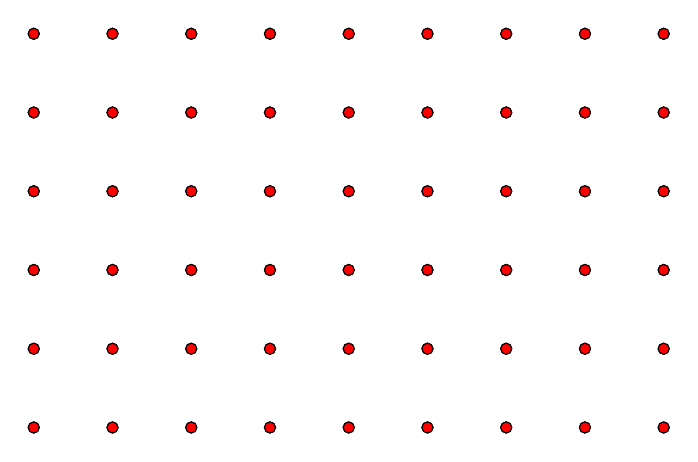
\begin{tikzpicture}[scale=1]%
\path[draw,radius=2pt,fill=red] (0.0,-7.0) circle;%
\path[draw,radius=2pt,fill=red] (1.0,-7.0) circle;%
\path[draw,radius=2pt,fill=red] (2.0,-7.0) circle;%
\path[draw,radius=2pt,fill=red] (3.0,-7.0) circle;%
\path[draw,radius=2pt,fill=red] (4.0,-7.0) circle;%
\path[draw,radius=2pt,fill=red] (5.0,-7.0) circle;%
\path[draw,radius=2pt,fill=red] (6.0,-7.0) circle;%
\path[draw,radius=2pt,fill=red] (7.0,-7.0) circle;%
\path[draw,radius=2pt,fill=red] (8.0,-7.0) circle;%
\path[draw,radius=2pt,fill=red] (0.0,-8.0) circle;%
\path[draw,radius=2pt,fill=red] (1.0,-8.0) circle;%
\path[draw,radius=2pt,fill=red] (2.0,-8.0) circle;%
\path[draw,radius=2pt,fill=red] (3.0,-8.0) circle;%
\path[draw,radius=2pt,fill=red] (4.0,-8.0) circle;%
\path[draw,radius=2pt,fill=red] (5.0,-8.0) circle;%
\path[draw,radius=2pt,fill=red] (6.0,-8.0) circle;%
\path[draw,radius=2pt,fill=red] (7.0,-8.0) circle;%
\path[draw,radius=2pt,fill=red] (8.0,-8.0) circle;%
\path[draw,radius=2pt,fill=red] (0.0,-9.0) circle;%
\path[draw,radius=2pt,fill=red] (1.0,-9.0) circle;%
\path[draw,radius=2pt,fill=red] (2.0,-9.0) circle;%
\path[draw,radius=2pt,fill=red] (3.0,-9.0) circle;%
\path[draw,radius=2pt,fill=red] (4.0,-9.0) circle;%
\path[draw,radius=2pt,fill=red] (5.0,-9.0) circle;%
\path[draw,radius=2pt,fill=red] (6.0,-9.0) circle;%
\path[draw,radius=2pt,fill=red] (7.0,-9.0) circle;%
\path[draw,radius=2pt,fill=red] (8.0,-9.0) circle;%
\path[draw,radius=2pt,fill=red] (0.0,-10.0) circle;%
\path[draw,radius=2pt,fill=red] (1.0,-10.0) circle;%
\path[draw,radius=2pt,fill=red] (2.0,-10.0) circle;%
\path[draw,radius=2pt,fill=red] (3.0,-10.0) circle;%
\path[draw,radius=2pt,fill=red] (4.0,-10.0) circle;%
\path[draw,radius=2pt,fill=red] (5.0,-10.0) circle;%
\path[draw,radius=2pt,fill=red] (6.0,-10.0) circle;%
\path[draw,radius=2pt,fill=red] (7.0,-10.0) circle;%
\path[draw,radius=2pt,fill=red] (8.0,-10.0) circle;%
\path[draw,radius=2pt,fill=red] (0.0,-11.0) circle;%
\path[draw,radius=2pt,fill=red] (1.0,-11.0) circle;%
\path[draw,radius=2pt,fill=red] (2.0,-11.0) circle;%
\path[draw,radius=2pt,fill=red] (3.0,-11.0) circle;%
\path[draw,radius=2pt,fill=red] (4.0,-11.0) circle;%
\path[draw,radius=2pt,fill=red] (5.0,-11.0) circle;%
\path[draw,radius=2pt,fill=red] (6.0,-11.0) circle;%
\path[draw,radius=2pt,fill=red] (7.0,-11.0) circle;%
\path[draw,radius=2pt,fill=red] (8.0,-11.0) circle;%
\path[draw,radius=2pt,fill=red] (0.0,-12.0) circle;%
\path[draw,radius=2pt,fill=red] (1.0,-12.0) circle;%
\path[draw,radius=2pt,fill=red] (2.0,-12.0) circle;%
\path[draw,radius=2pt,fill=red] (3.0,-12.0) circle;%
\path[draw,radius=2pt,fill=red] (4.0,-12.0) circle;%
\path[draw,radius=2pt,fill=red] (5.0,-12.0) circle;%
\path[draw,radius=2pt,fill=red] (6.0,-12.0) circle;%
\path[draw,radius=2pt,fill=red] (7.0,-12.0) circle;%
\path[draw,radius=2pt,fill=red] (8.0,-12.0) circle;%
\path[draw,radius=2pt,fill=red] (0.0,-7.0) circle;%
\path[draw,radius=2pt,fill=red] (1.0,-7.0) circle;%
\path[draw,radius=2pt,fill=red] (2.0,-7.0) circle;%
\path[draw,radius=2pt,fill=red] (3.0,-7.0) circle;%
\path[draw,radius=2pt,fill=red] (4.0,-7.0) circle;%
\path[draw,radius=2pt,fill=red] (5.0,-7.0) circle;%
\path[draw,radius=2pt,fill=red] (6.0,-7.0) circle;%
\path[draw,radius=2pt,fill=red] (7.0,-7.0) circle;%
\path[draw,radius=2pt,fill=red] (8.0,-7.0) circle;%
\path[draw,radius=2pt,fill=red] (0.0,-8.0) circle;%
\path[draw,radius=2pt,fill=red] (1.0,-8.0) circle;%
\path[draw,radius=2pt,fill=red] (2.0,-8.0) circle;%
\path[draw,radius=2pt,fill=red] (3.0,-8.0) circle;%
\path[draw,radius=2pt,fill=red] (4.0,-8.0) circle;%
\path[draw,radius=2pt,fill=red] (5.0,-8.0) circle;%
\path[draw,radius=2pt,fill=red] (6.0,-8.0) circle;%
\path[draw,radius=2pt,fill=red] (7.0,-8.0) circle;%
\path[draw,radius=2pt,fill=red] (8.0,-8.0) circle;%
\path[draw,radius=2pt,fill=red] (0.0,-9.0) circle;%
\path[draw,radius=2pt,fill=red] (1.0,-9.0) circle;%
\path[draw,radius=2pt,fill=red] (2.0,-9.0) circle;%
\path[draw,radius=2pt,fill=red] (3.0,-9.0) circle;%
\path[draw,radius=2pt,fill=red] (4.0,-9.0) circle;%
\path[draw,radius=2pt,fill=red] (5.0,-9.0) circle;%
\path[draw,radius=2pt,fill=red] (6.0,-9.0) circle;%
\path[draw,radius=2pt,fill=red] (7.0,-9.0) circle;%
\path[draw,radius=2pt,fill=red] (8.0,-9.0) circle;%
\path[draw,radius=2pt,fill=red] (0.0,-10.0) circle;%
\path[draw,radius=2pt,fill=red] (1.0,-10.0) circle;%
\path[draw,radius=2pt,fill=red] (2.0,-10.0) circle;%
\path[draw,radius=2pt,fill=red] (3.0,-10.0) circle;%
\path[draw,radius=2pt,fill=red] (4.0,-10.0) circle;%
\path[draw,radius=2pt,fill=red] (5.0,-10.0) circle;%
\path[draw,radius=2pt,fill=red] (6.0,-10.0) circle;%
\path[draw,radius=2pt,fill=red] (7.0,-10.0) circle;%
\path[draw,radius=2pt,fill=red] (8.0,-10.0) circle;%
\path[draw,radius=2pt,fill=red] (0.0,-11.0) circle;%
\path[draw,radius=2pt,fill=red] (1.0,-11.0) circle;%
\path[draw,radius=2pt,fill=red] (2.0,-11.0) circle;%
\path[draw,radius=2pt,fill=red] (3.0,-11.0) circle;%
\path[draw,radius=2pt,fill=red] (4.0,-11.0) circle;%
\path[draw,radius=2pt,fill=red] (5.0,-11.0) circle;%
\path[draw,radius=2pt,fill=red] (6.0,-11.0) circle;%
\path[draw,radius=2pt,fill=red] (7.0,-11.0) circle;%
\path[draw,radius=2pt,fill=red] (8.0,-11.0) circle;%
\path[draw,radius=2pt,fill=red] (0.0,-12.0) circle;%
\path[draw,radius=2pt,fill=red] (1.0,-12.0) circle;%
\path[draw,radius=2pt,fill=red] (2.0,-12.0) circle;%
\path[draw,radius=2pt,fill=red] (3.0,-12.0) circle;%
\path[draw,radius=2pt,fill=red] (4.0,-12.0) circle;%
\path[draw,radius=2pt,fill=red] (5.0,-12.0) circle;%
\path[draw,radius=2pt,fill=red] (6.0,-12.0) circle;%
\path[draw,radius=2pt,fill=red] (7.0,-12.0) circle;%
\path[draw,radius=2pt,fill=red] (8.0,-12.0) circle;%
\end{tikzpicture}%
\hspace*{1in}%
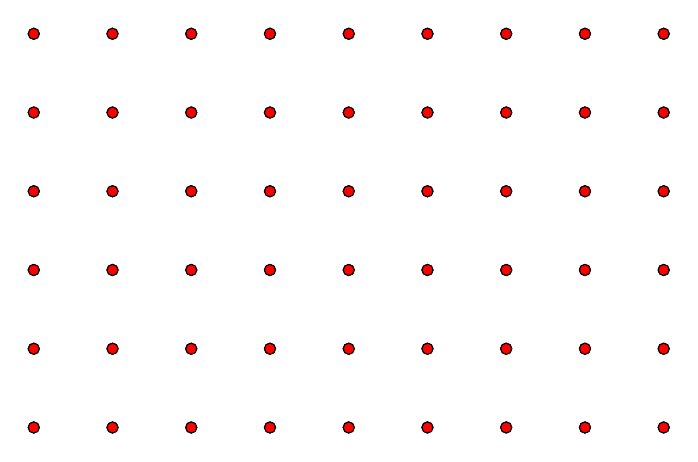
\begin{tikzpicture}[scale=1]%
\path[draw,radius=2pt] (8.0,-7.0) circle;%
\path[draw,radius=2pt,fill=red] (0.0,-7.0) circle;%
\path[draw,radius=2pt,fill=red] (1.0,-7.0) circle;%
\path[draw,radius=2pt,fill=red] (2.0,-7.0) circle;%
\path[draw,radius=2pt,fill=red] (3.0,-7.0) circle;%
\path[draw,radius=2pt,fill=red] (4.0,-7.0) circle;%
\path[draw,radius=2pt,fill=red] (5.0,-7.0) circle;%
\path[draw,radius=2pt,fill=red] (6.0,-7.0) circle;%
\path[draw,radius=2pt,fill=red] (7.0,-7.0) circle;%
\path[draw,radius=2pt,fill=red] (8.0,-7.0) circle;%
\path[draw,radius=2pt,fill=red] (0.0,-8.0) circle;%
\path[draw,radius=2pt,fill=red] (1.0,-8.0) circle;%
\path[draw,radius=2pt,fill=red] (2.0,-8.0) circle;%
\path[draw,radius=2pt,fill=red] (3.0,-8.0) circle;%
\path[draw,radius=2pt,fill=red] (4.0,-8.0) circle;%
\path[draw,radius=2pt,fill=red] (5.0,-8.0) circle;%
\path[draw,radius=2pt,fill=red] (6.0,-8.0) circle;%
\path[draw,radius=2pt,fill=red] (7.0,-8.0) circle;%
\path[draw,radius=2pt,fill=red] (8.0,-8.0) circle;%
\path[draw,radius=2pt,fill=red] (0.0,-9.0) circle;%
\path[draw,radius=2pt,fill=red] (1.0,-9.0) circle;%
\path[draw,radius=2pt,fill=red] (2.0,-9.0) circle;%
\path[draw,radius=2pt,fill=red] (3.0,-9.0) circle;%
\path[draw,radius=2pt,fill=red] (4.0,-9.0) circle;%
\path[draw,radius=2pt,fill=red] (5.0,-9.0) circle;%
\path[draw,radius=2pt,fill=red] (6.0,-9.0) circle;%
\path[draw,radius=2pt,fill=red] (7.0,-9.0) circle;%
\path[draw,radius=2pt,fill=red] (8.0,-9.0) circle;%
\path[draw,radius=2pt,fill=red] (0.0,-10.0) circle;%
\path[draw,radius=2pt,fill=red] (1.0,-10.0) circle;%
\path[draw,radius=2pt,fill=red] (2.0,-10.0) circle;%
\path[draw,radius=2pt,fill=red] (3.0,-10.0) circle;%
\path[draw,radius=2pt,fill=red] (4.0,-10.0) circle;%
\path[draw,radius=2pt,fill=red] (5.0,-10.0) circle;%
\path[draw,radius=2pt,fill=red] (6.0,-10.0) circle;%
\path[draw,radius=2pt,fill=red] (7.0,-10.0) circle;%
\path[draw,radius=2pt,fill=red] (8.0,-10.0) circle;%
\path[draw,radius=2pt,fill=red] (0.0,-11.0) circle;%
\path[draw,radius=2pt,fill=red] (1.0,-11.0) circle;%
\path[draw,radius=2pt,fill=red] (2.0,-11.0) circle;%
\path[draw,radius=2pt,fill=red] (3.0,-11.0) circle;%
\path[draw,radius=2pt,fill=red] (4.0,-11.0) circle;%
\path[draw,radius=2pt,fill=red] (5.0,-11.0) circle;%
\path[draw,radius=2pt,fill=red] (6.0,-11.0) circle;%
\path[draw,radius=2pt,fill=red] (7.0,-11.0) circle;%
\path[draw,radius=2pt,fill=red] (8.0,-11.0) circle;%
\path[draw,radius=2pt,fill=red] (0.0,-12.0) circle;%
\path[draw,radius=2pt,fill=red] (1.0,-12.0) circle;%
\path[draw,radius=2pt,fill=red] (2.0,-12.0) circle;%
\path[draw,radius=2pt,fill=red] (3.0,-12.0) circle;%
\path[draw,radius=2pt,fill=red] (4.0,-12.0) circle;%
\path[draw,radius=2pt,fill=red] (5.0,-12.0) circle;%
\path[draw,radius=2pt,fill=red] (6.0,-12.0) circle;%
\path[draw,radius=2pt,fill=red] (7.0,-12.0) circle;%
\path[draw,radius=2pt,fill=red] (8.0,-12.0) circle;%
\path[draw,radius=2pt,fill=red] (0.0,-7.0) circle;%
\path[draw,radius=2pt,fill=red] (1.0,-7.0) circle;%
\path[draw,radius=2pt,fill=red] (2.0,-7.0) circle;%
\path[draw,radius=2pt,fill=red] (3.0,-7.0) circle;%
\path[draw,radius=2pt,fill=red] (4.0,-7.0) circle;%
\path[draw,radius=2pt,fill=red] (5.0,-7.0) circle;%
\path[draw,radius=2pt,fill=red] (6.0,-7.0) circle;%
\path[draw,radius=2pt,fill=red] (7.0,-7.0) circle;%
\path[draw,radius=2pt,fill=red] (0.0,-8.0) circle;%
\path[draw,radius=2pt,fill=red] (1.0,-8.0) circle;%
\path[draw,radius=2pt,fill=red] (2.0,-8.0) circle;%
\path[draw,radius=2pt,fill=red] (3.0,-8.0) circle;%
\path[draw,radius=2pt,fill=red] (4.0,-8.0) circle;%
\path[draw,radius=2pt,fill=red] (5.0,-8.0) circle;%
\path[draw,radius=2pt,fill=red] (6.0,-8.0) circle;%
\path[draw,radius=2pt,fill=red] (7.0,-8.0) circle;%
\path[draw,radius=2pt,fill=red] (8.0,-8.0) circle;%
\path[draw,radius=2pt,fill=red] (0.0,-9.0) circle;%
\path[draw,radius=2pt,fill=red] (1.0,-9.0) circle;%
\path[draw,radius=2pt,fill=red] (2.0,-9.0) circle;%
\path[draw,radius=2pt,fill=red] (3.0,-9.0) circle;%
\path[draw,radius=2pt,fill=red] (4.0,-9.0) circle;%
\path[draw,radius=2pt,fill=red] (5.0,-9.0) circle;%
\path[draw,radius=2pt,fill=red] (6.0,-9.0) circle;%
\path[draw,radius=2pt,fill=red] (7.0,-9.0) circle;%
\path[draw,radius=2pt,fill=red] (8.0,-9.0) circle;%
\path[draw,radius=2pt,fill=red] (0.0,-10.0) circle;%
\path[draw,radius=2pt,fill=red] (1.0,-10.0) circle;%
\path[draw,radius=2pt,fill=red] (2.0,-10.0) circle;%
\path[draw,radius=2pt,fill=red] (3.0,-10.0) circle;%
\path[draw,radius=2pt,fill=red] (4.0,-10.0) circle;%
\path[draw,radius=2pt,fill=red] (5.0,-10.0) circle;%
\path[draw,radius=2pt,fill=red] (6.0,-10.0) circle;%
\path[draw,radius=2pt,fill=red] (7.0,-10.0) circle;%
\path[draw,radius=2pt,fill=red] (8.0,-10.0) circle;%
\path[draw,radius=2pt,fill=red] (0.0,-11.0) circle;%
\path[draw,radius=2pt,fill=red] (1.0,-11.0) circle;%
\path[draw,radius=2pt,fill=red] (2.0,-11.0) circle;%
\path[draw,radius=2pt,fill=red] (3.0,-11.0) circle;%
\path[draw,radius=2pt,fill=red] (4.0,-11.0) circle;%
\path[draw,radius=2pt,fill=red] (5.0,-11.0) circle;%
\path[draw,radius=2pt,fill=red] (6.0,-11.0) circle;%
\path[draw,radius=2pt,fill=red] (7.0,-11.0) circle;%
\path[draw,radius=2pt,fill=red] (8.0,-11.0) circle;%
\path[draw,radius=2pt,fill=red] (0.0,-12.0) circle;%
\path[draw,radius=2pt,fill=red] (1.0,-12.0) circle;%
\path[draw,radius=2pt,fill=red] (2.0,-12.0) circle;%
\path[draw,radius=2pt,fill=red] (3.0,-12.0) circle;%
\path[draw,radius=2pt,fill=red] (4.0,-12.0) circle;%
\path[draw,radius=2pt,fill=red] (5.0,-12.0) circle;%
\path[draw,radius=2pt,fill=red] (6.0,-12.0) circle;%
\path[draw,radius=2pt,fill=red] (7.0,-12.0) circle;%
\path[draw,radius=2pt,fill=red] (8.0,-12.0) circle;%
\end{tikzpicture}%
\hspace*{1in}%
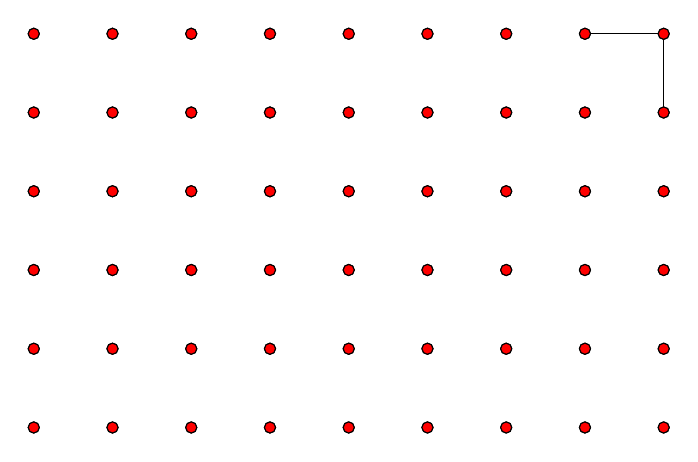
\begin{tikzpicture}[scale=1]%
\path[draw] (7.0,-7.0) -- (8.0,-7.0);%
\path[draw,radius=2pt] (7.0,-7.0) circle;%
\path[draw] (8.0,-7.0) -- (8.0,-8.0);%
\path[draw] (8.0,-7.0) -- (7.0,-7.0);%
\path[draw,radius=2pt] (8.0,-7.0) circle;%
\path[draw] (8.0,-8.0) -- (8.0,-7.0);%
\path[draw,radius=2pt] (8.0,-8.0) circle;%
\path[draw,radius=2pt,fill=red] (0.0,-7.0) circle;%
\path[draw,radius=2pt,fill=red] (1.0,-7.0) circle;%
\path[draw,radius=2pt,fill=red] (2.0,-7.0) circle;%
\path[draw,radius=2pt,fill=red] (3.0,-7.0) circle;%
\path[draw,radius=2pt,fill=red] (4.0,-7.0) circle;%
\path[draw,radius=2pt,fill=red] (5.0,-7.0) circle;%
\path[draw,radius=2pt,fill=red] (6.0,-7.0) circle;%
\path[draw,radius=2pt,fill=red] (7.0,-7.0) circle;%
\path[draw,radius=2pt,fill=red] (8.0,-7.0) circle;%
\path[draw,radius=2pt,fill=red] (0.0,-8.0) circle;%
\path[draw,radius=2pt,fill=red] (1.0,-8.0) circle;%
\path[draw,radius=2pt,fill=red] (2.0,-8.0) circle;%
\path[draw,radius=2pt,fill=red] (3.0,-8.0) circle;%
\path[draw,radius=2pt,fill=red] (4.0,-8.0) circle;%
\path[draw,radius=2pt,fill=red] (5.0,-8.0) circle;%
\path[draw,radius=2pt,fill=red] (6.0,-8.0) circle;%
\path[draw,radius=2pt,fill=red] (7.0,-8.0) circle;%
\path[draw,radius=2pt,fill=red] (8.0,-8.0) circle;%
\path[draw,radius=2pt,fill=red] (0.0,-9.0) circle;%
\path[draw,radius=2pt,fill=red] (1.0,-9.0) circle;%
\path[draw,radius=2pt,fill=red] (2.0,-9.0) circle;%
\path[draw,radius=2pt,fill=red] (3.0,-9.0) circle;%
\path[draw,radius=2pt,fill=red] (4.0,-9.0) circle;%
\path[draw,radius=2pt,fill=red] (5.0,-9.0) circle;%
\path[draw,radius=2pt,fill=red] (6.0,-9.0) circle;%
\path[draw,radius=2pt,fill=red] (7.0,-9.0) circle;%
\path[draw,radius=2pt,fill=red] (8.0,-9.0) circle;%
\path[draw,radius=2pt,fill=red] (0.0,-10.0) circle;%
\path[draw,radius=2pt,fill=red] (1.0,-10.0) circle;%
\path[draw,radius=2pt,fill=red] (2.0,-10.0) circle;%
\path[draw,radius=2pt,fill=red] (3.0,-10.0) circle;%
\path[draw,radius=2pt,fill=red] (4.0,-10.0) circle;%
\path[draw,radius=2pt,fill=red] (5.0,-10.0) circle;%
\path[draw,radius=2pt,fill=red] (6.0,-10.0) circle;%
\path[draw,radius=2pt,fill=red] (7.0,-10.0) circle;%
\path[draw,radius=2pt,fill=red] (8.0,-10.0) circle;%
\path[draw,radius=2pt,fill=red] (0.0,-11.0) circle;%
\path[draw,radius=2pt,fill=red] (1.0,-11.0) circle;%
\path[draw,radius=2pt,fill=red] (2.0,-11.0) circle;%
\path[draw,radius=2pt,fill=red] (3.0,-11.0) circle;%
\path[draw,radius=2pt,fill=red] (4.0,-11.0) circle;%
\path[draw,radius=2pt,fill=red] (5.0,-11.0) circle;%
\path[draw,radius=2pt,fill=red] (6.0,-11.0) circle;%
\path[draw,radius=2pt,fill=red] (7.0,-11.0) circle;%
\path[draw,radius=2pt,fill=red] (8.0,-11.0) circle;%
\path[draw,radius=2pt,fill=red] (0.0,-12.0) circle;%
\path[draw,radius=2pt,fill=red] (1.0,-12.0) circle;%
\path[draw,radius=2pt,fill=red] (2.0,-12.0) circle;%
\path[draw,radius=2pt,fill=red] (3.0,-12.0) circle;%
\path[draw,radius=2pt,fill=red] (4.0,-12.0) circle;%
\path[draw,radius=2pt,fill=red] (5.0,-12.0) circle;%
\path[draw,radius=2pt,fill=red] (6.0,-12.0) circle;%
\path[draw,radius=2pt,fill=red] (7.0,-12.0) circle;%
\path[draw,radius=2pt,fill=red] (8.0,-12.0) circle;%
\path[draw,radius=2pt,fill=red] (0.0,-7.0) circle;%
\path[draw,radius=2pt,fill=red] (1.0,-7.0) circle;%
\path[draw,radius=2pt,fill=red] (2.0,-7.0) circle;%
\path[draw,radius=2pt,fill=red] (3.0,-7.0) circle;%
\path[draw,radius=2pt,fill=red] (4.0,-7.0) circle;%
\path[draw,radius=2pt,fill=red] (5.0,-7.0) circle;%
\path[draw,radius=2pt,fill=red] (6.0,-7.0) circle;%
\path[draw,radius=2pt,fill=red] (0.0,-8.0) circle;%
\path[draw,radius=2pt,fill=red] (1.0,-8.0) circle;%
\path[draw,radius=2pt,fill=red] (2.0,-8.0) circle;%
\path[draw,radius=2pt,fill=red] (3.0,-8.0) circle;%
\path[draw,radius=2pt,fill=red] (4.0,-8.0) circle;%
\path[draw,radius=2pt,fill=red] (5.0,-8.0) circle;%
\path[draw,radius=2pt,fill=red] (6.0,-8.0) circle;%
\path[draw,radius=2pt,fill=red] (7.0,-8.0) circle;%
\path[draw,radius=2pt,fill=red] (0.0,-9.0) circle;%
\path[draw,radius=2pt,fill=red] (1.0,-9.0) circle;%
\path[draw,radius=2pt,fill=red] (2.0,-9.0) circle;%
\path[draw,radius=2pt,fill=red] (3.0,-9.0) circle;%
\path[draw,radius=2pt,fill=red] (4.0,-9.0) circle;%
\path[draw,radius=2pt,fill=red] (5.0,-9.0) circle;%
\path[draw,radius=2pt,fill=red] (6.0,-9.0) circle;%
\path[draw,radius=2pt,fill=red] (7.0,-9.0) circle;%
\path[draw,radius=2pt,fill=red] (8.0,-9.0) circle;%
\path[draw,radius=2pt,fill=red] (0.0,-10.0) circle;%
\path[draw,radius=2pt,fill=red] (1.0,-10.0) circle;%
\path[draw,radius=2pt,fill=red] (2.0,-10.0) circle;%
\path[draw,radius=2pt,fill=red] (3.0,-10.0) circle;%
\path[draw,radius=2pt,fill=red] (4.0,-10.0) circle;%
\path[draw,radius=2pt,fill=red] (5.0,-10.0) circle;%
\path[draw,radius=2pt,fill=red] (6.0,-10.0) circle;%
\path[draw,radius=2pt,fill=red] (7.0,-10.0) circle;%
\path[draw,radius=2pt,fill=red] (8.0,-10.0) circle;%
\path[draw,radius=2pt,fill=red] (0.0,-11.0) circle;%
\path[draw,radius=2pt,fill=red] (1.0,-11.0) circle;%
\path[draw,radius=2pt,fill=red] (2.0,-11.0) circle;%
\path[draw,radius=2pt,fill=red] (3.0,-11.0) circle;%
\path[draw,radius=2pt,fill=red] (4.0,-11.0) circle;%
\path[draw,radius=2pt,fill=red] (5.0,-11.0) circle;%
\path[draw,radius=2pt,fill=red] (6.0,-11.0) circle;%
\path[draw,radius=2pt,fill=red] (7.0,-11.0) circle;%
\path[draw,radius=2pt,fill=red] (8.0,-11.0) circle;%
\path[draw,radius=2pt,fill=red] (0.0,-12.0) circle;%
\path[draw,radius=2pt,fill=red] (1.0,-12.0) circle;%
\path[draw,radius=2pt,fill=red] (2.0,-12.0) circle;%
\path[draw,radius=2pt,fill=red] (3.0,-12.0) circle;%
\path[draw,radius=2pt,fill=red] (4.0,-12.0) circle;%
\path[draw,radius=2pt,fill=red] (5.0,-12.0) circle;%
\path[draw,radius=2pt,fill=red] (6.0,-12.0) circle;%
\path[draw,radius=2pt,fill=red] (7.0,-12.0) circle;%
\path[draw,radius=2pt,fill=red] (8.0,-12.0) circle;%
\end{tikzpicture}%
\newline%
\hspace*{1in}%
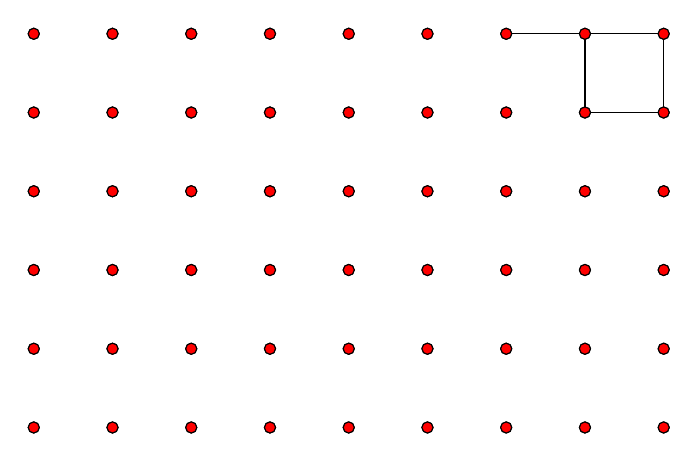
\begin{tikzpicture}[scale=1]%
\path[draw] (6.0,-7.0) -- (7.0,-7.0);%
\path[draw,radius=2pt] (6.0,-7.0) circle;%
\path[draw] (7.0,-7.0) -- (7.0,-8.0);%
\path[draw] (7.0,-7.0) -- (6.0,-7.0);%
\path[draw] (7.0,-7.0) -- (8.0,-7.0);%
\path[draw,radius=2pt] (7.0,-7.0) circle;%
\path[draw] (8.0,-7.0) -- (8.0,-8.0);%
\path[draw] (8.0,-7.0) -- (7.0,-7.0);%
\path[draw,radius=2pt] (8.0,-7.0) circle;%
\path[draw] (7.0,-8.0) -- (7.0,-7.0);%
\path[draw] (7.0,-8.0) -- (8.0,-8.0);%
\path[draw,radius=2pt] (7.0,-8.0) circle;%
\path[draw] (8.0,-8.0) -- (8.0,-7.0);%
\path[draw] (8.0,-8.0) -- (7.0,-8.0);%
\path[draw,radius=2pt] (8.0,-8.0) circle;%
\path[draw,radius=2pt,fill=red] (0.0,-7.0) circle;%
\path[draw,radius=2pt,fill=red] (1.0,-7.0) circle;%
\path[draw,radius=2pt,fill=red] (2.0,-7.0) circle;%
\path[draw,radius=2pt,fill=red] (3.0,-7.0) circle;%
\path[draw,radius=2pt,fill=red] (4.0,-7.0) circle;%
\path[draw,radius=2pt,fill=red] (5.0,-7.0) circle;%
\path[draw,radius=2pt,fill=red] (6.0,-7.0) circle;%
\path[draw,radius=2pt,fill=red] (7.0,-7.0) circle;%
\path[draw,radius=2pt,fill=red] (8.0,-7.0) circle;%
\path[draw,radius=2pt,fill=red] (0.0,-8.0) circle;%
\path[draw,radius=2pt,fill=red] (1.0,-8.0) circle;%
\path[draw,radius=2pt,fill=red] (2.0,-8.0) circle;%
\path[draw,radius=2pt,fill=red] (3.0,-8.0) circle;%
\path[draw,radius=2pt,fill=red] (4.0,-8.0) circle;%
\path[draw,radius=2pt,fill=red] (5.0,-8.0) circle;%
\path[draw,radius=2pt,fill=red] (6.0,-8.0) circle;%
\path[draw,radius=2pt,fill=red] (7.0,-8.0) circle;%
\path[draw,radius=2pt,fill=red] (8.0,-8.0) circle;%
\path[draw,radius=2pt,fill=red] (0.0,-9.0) circle;%
\path[draw,radius=2pt,fill=red] (1.0,-9.0) circle;%
\path[draw,radius=2pt,fill=red] (2.0,-9.0) circle;%
\path[draw,radius=2pt,fill=red] (3.0,-9.0) circle;%
\path[draw,radius=2pt,fill=red] (4.0,-9.0) circle;%
\path[draw,radius=2pt,fill=red] (5.0,-9.0) circle;%
\path[draw,radius=2pt,fill=red] (6.0,-9.0) circle;%
\path[draw,radius=2pt,fill=red] (7.0,-9.0) circle;%
\path[draw,radius=2pt,fill=red] (8.0,-9.0) circle;%
\path[draw,radius=2pt,fill=red] (0.0,-10.0) circle;%
\path[draw,radius=2pt,fill=red] (1.0,-10.0) circle;%
\path[draw,radius=2pt,fill=red] (2.0,-10.0) circle;%
\path[draw,radius=2pt,fill=red] (3.0,-10.0) circle;%
\path[draw,radius=2pt,fill=red] (4.0,-10.0) circle;%
\path[draw,radius=2pt,fill=red] (5.0,-10.0) circle;%
\path[draw,radius=2pt,fill=red] (6.0,-10.0) circle;%
\path[draw,radius=2pt,fill=red] (7.0,-10.0) circle;%
\path[draw,radius=2pt,fill=red] (8.0,-10.0) circle;%
\path[draw,radius=2pt,fill=red] (0.0,-11.0) circle;%
\path[draw,radius=2pt,fill=red] (1.0,-11.0) circle;%
\path[draw,radius=2pt,fill=red] (2.0,-11.0) circle;%
\path[draw,radius=2pt,fill=red] (3.0,-11.0) circle;%
\path[draw,radius=2pt,fill=red] (4.0,-11.0) circle;%
\path[draw,radius=2pt,fill=red] (5.0,-11.0) circle;%
\path[draw,radius=2pt,fill=red] (6.0,-11.0) circle;%
\path[draw,radius=2pt,fill=red] (7.0,-11.0) circle;%
\path[draw,radius=2pt,fill=red] (8.0,-11.0) circle;%
\path[draw,radius=2pt,fill=red] (0.0,-12.0) circle;%
\path[draw,radius=2pt,fill=red] (1.0,-12.0) circle;%
\path[draw,radius=2pt,fill=red] (2.0,-12.0) circle;%
\path[draw,radius=2pt,fill=red] (3.0,-12.0) circle;%
\path[draw,radius=2pt,fill=red] (4.0,-12.0) circle;%
\path[draw,radius=2pt,fill=red] (5.0,-12.0) circle;%
\path[draw,radius=2pt,fill=red] (6.0,-12.0) circle;%
\path[draw,radius=2pt,fill=red] (7.0,-12.0) circle;%
\path[draw,radius=2pt,fill=red] (8.0,-12.0) circle;%
\path[draw,radius=2pt,fill=red] (0.0,-7.0) circle;%
\path[draw,radius=2pt,fill=red] (1.0,-7.0) circle;%
\path[draw,radius=2pt,fill=red] (2.0,-7.0) circle;%
\path[draw,radius=2pt,fill=red] (3.0,-7.0) circle;%
\path[draw,radius=2pt,fill=red] (4.0,-7.0) circle;%
\path[draw,radius=2pt,fill=red] (5.0,-7.0) circle;%
\path[draw,radius=2pt,fill=red] (0.0,-8.0) circle;%
\path[draw,radius=2pt,fill=red] (1.0,-8.0) circle;%
\path[draw,radius=2pt,fill=red] (2.0,-8.0) circle;%
\path[draw,radius=2pt,fill=red] (3.0,-8.0) circle;%
\path[draw,radius=2pt,fill=red] (4.0,-8.0) circle;%
\path[draw,radius=2pt,fill=red] (5.0,-8.0) circle;%
\path[draw,radius=2pt,fill=red] (6.0,-8.0) circle;%
\path[draw,radius=2pt,fill=red] (0.0,-9.0) circle;%
\path[draw,radius=2pt,fill=red] (1.0,-9.0) circle;%
\path[draw,radius=2pt,fill=red] (2.0,-9.0) circle;%
\path[draw,radius=2pt,fill=red] (3.0,-9.0) circle;%
\path[draw,radius=2pt,fill=red] (4.0,-9.0) circle;%
\path[draw,radius=2pt,fill=red] (5.0,-9.0) circle;%
\path[draw,radius=2pt,fill=red] (6.0,-9.0) circle;%
\path[draw,radius=2pt,fill=red] (7.0,-9.0) circle;%
\path[draw,radius=2pt,fill=red] (8.0,-9.0) circle;%
\path[draw,radius=2pt,fill=red] (0.0,-10.0) circle;%
\path[draw,radius=2pt,fill=red] (1.0,-10.0) circle;%
\path[draw,radius=2pt,fill=red] (2.0,-10.0) circle;%
\path[draw,radius=2pt,fill=red] (3.0,-10.0) circle;%
\path[draw,radius=2pt,fill=red] (4.0,-10.0) circle;%
\path[draw,radius=2pt,fill=red] (5.0,-10.0) circle;%
\path[draw,radius=2pt,fill=red] (6.0,-10.0) circle;%
\path[draw,radius=2pt,fill=red] (7.0,-10.0) circle;%
\path[draw,radius=2pt,fill=red] (8.0,-10.0) circle;%
\path[draw,radius=2pt,fill=red] (0.0,-11.0) circle;%
\path[draw,radius=2pt,fill=red] (1.0,-11.0) circle;%
\path[draw,radius=2pt,fill=red] (2.0,-11.0) circle;%
\path[draw,radius=2pt,fill=red] (3.0,-11.0) circle;%
\path[draw,radius=2pt,fill=red] (4.0,-11.0) circle;%
\path[draw,radius=2pt,fill=red] (5.0,-11.0) circle;%
\path[draw,radius=2pt,fill=red] (6.0,-11.0) circle;%
\path[draw,radius=2pt,fill=red] (7.0,-11.0) circle;%
\path[draw,radius=2pt,fill=red] (8.0,-11.0) circle;%
\path[draw,radius=2pt,fill=red] (0.0,-12.0) circle;%
\path[draw,radius=2pt,fill=red] (1.0,-12.0) circle;%
\path[draw,radius=2pt,fill=red] (2.0,-12.0) circle;%
\path[draw,radius=2pt,fill=red] (3.0,-12.0) circle;%
\path[draw,radius=2pt,fill=red] (4.0,-12.0) circle;%
\path[draw,radius=2pt,fill=red] (5.0,-12.0) circle;%
\path[draw,radius=2pt,fill=red] (6.0,-12.0) circle;%
\path[draw,radius=2pt,fill=red] (7.0,-12.0) circle;%
\path[draw,radius=2pt,fill=red] (8.0,-12.0) circle;%
\end{tikzpicture}%
\hspace*{1in}%
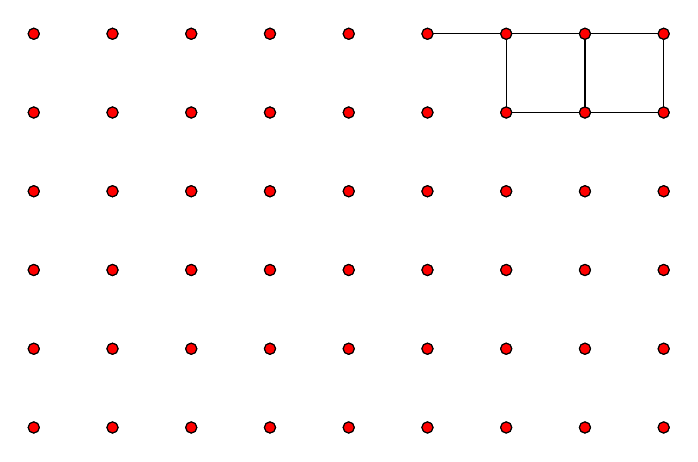
\begin{tikzpicture}[scale=1]%
\path[draw] (5.0,-7.0) -- (6.0,-7.0);%
\path[draw,radius=2pt] (5.0,-7.0) circle;%
\path[draw] (6.0,-7.0) -- (6.0,-8.0);%
\path[draw] (6.0,-7.0) -- (5.0,-7.0);%
\path[draw] (6.0,-7.0) -- (7.0,-7.0);%
\path[draw,radius=2pt] (6.0,-7.0) circle;%
\path[draw] (7.0,-7.0) -- (7.0,-8.0);%
\path[draw] (7.0,-7.0) -- (6.0,-7.0);%
\path[draw] (7.0,-7.0) -- (8.0,-7.0);%
\path[draw,radius=2pt] (7.0,-7.0) circle;%
\path[draw] (8.0,-7.0) -- (8.0,-8.0);%
\path[draw] (8.0,-7.0) -- (7.0,-7.0);%
\path[draw,radius=2pt] (8.0,-7.0) circle;%
\path[draw] (6.0,-8.0) -- (6.0,-7.0);%
\path[draw] (6.0,-8.0) -- (7.0,-8.0);%
\path[draw,radius=2pt] (6.0,-8.0) circle;%
\path[draw] (7.0,-8.0) -- (7.0,-7.0);%
\path[draw] (7.0,-8.0) -- (6.0,-8.0);%
\path[draw] (7.0,-8.0) -- (8.0,-8.0);%
\path[draw,radius=2pt] (7.0,-8.0) circle;%
\path[draw] (8.0,-8.0) -- (8.0,-7.0);%
\path[draw] (8.0,-8.0) -- (7.0,-8.0);%
\path[draw,radius=2pt] (8.0,-8.0) circle;%
\path[draw,radius=2pt,fill=red] (0.0,-7.0) circle;%
\path[draw,radius=2pt,fill=red] (1.0,-7.0) circle;%
\path[draw,radius=2pt,fill=red] (2.0,-7.0) circle;%
\path[draw,radius=2pt,fill=red] (3.0,-7.0) circle;%
\path[draw,radius=2pt,fill=red] (4.0,-7.0) circle;%
\path[draw,radius=2pt,fill=red] (5.0,-7.0) circle;%
\path[draw,radius=2pt,fill=red] (6.0,-7.0) circle;%
\path[draw,radius=2pt,fill=red] (7.0,-7.0) circle;%
\path[draw,radius=2pt,fill=red] (8.0,-7.0) circle;%
\path[draw,radius=2pt,fill=red] (0.0,-8.0) circle;%
\path[draw,radius=2pt,fill=red] (1.0,-8.0) circle;%
\path[draw,radius=2pt,fill=red] (2.0,-8.0) circle;%
\path[draw,radius=2pt,fill=red] (3.0,-8.0) circle;%
\path[draw,radius=2pt,fill=red] (4.0,-8.0) circle;%
\path[draw,radius=2pt,fill=red] (5.0,-8.0) circle;%
\path[draw,radius=2pt,fill=red] (6.0,-8.0) circle;%
\path[draw,radius=2pt,fill=red] (7.0,-8.0) circle;%
\path[draw,radius=2pt,fill=red] (8.0,-8.0) circle;%
\path[draw,radius=2pt,fill=red] (0.0,-9.0) circle;%
\path[draw,radius=2pt,fill=red] (1.0,-9.0) circle;%
\path[draw,radius=2pt,fill=red] (2.0,-9.0) circle;%
\path[draw,radius=2pt,fill=red] (3.0,-9.0) circle;%
\path[draw,radius=2pt,fill=red] (4.0,-9.0) circle;%
\path[draw,radius=2pt,fill=red] (5.0,-9.0) circle;%
\path[draw,radius=2pt,fill=red] (6.0,-9.0) circle;%
\path[draw,radius=2pt,fill=red] (7.0,-9.0) circle;%
\path[draw,radius=2pt,fill=red] (8.0,-9.0) circle;%
\path[draw,radius=2pt,fill=red] (0.0,-10.0) circle;%
\path[draw,radius=2pt,fill=red] (1.0,-10.0) circle;%
\path[draw,radius=2pt,fill=red] (2.0,-10.0) circle;%
\path[draw,radius=2pt,fill=red] (3.0,-10.0) circle;%
\path[draw,radius=2pt,fill=red] (4.0,-10.0) circle;%
\path[draw,radius=2pt,fill=red] (5.0,-10.0) circle;%
\path[draw,radius=2pt,fill=red] (6.0,-10.0) circle;%
\path[draw,radius=2pt,fill=red] (7.0,-10.0) circle;%
\path[draw,radius=2pt,fill=red] (8.0,-10.0) circle;%
\path[draw,radius=2pt,fill=red] (0.0,-11.0) circle;%
\path[draw,radius=2pt,fill=red] (1.0,-11.0) circle;%
\path[draw,radius=2pt,fill=red] (2.0,-11.0) circle;%
\path[draw,radius=2pt,fill=red] (3.0,-11.0) circle;%
\path[draw,radius=2pt,fill=red] (4.0,-11.0) circle;%
\path[draw,radius=2pt,fill=red] (5.0,-11.0) circle;%
\path[draw,radius=2pt,fill=red] (6.0,-11.0) circle;%
\path[draw,radius=2pt,fill=red] (7.0,-11.0) circle;%
\path[draw,radius=2pt,fill=red] (8.0,-11.0) circle;%
\path[draw,radius=2pt,fill=red] (0.0,-12.0) circle;%
\path[draw,radius=2pt,fill=red] (1.0,-12.0) circle;%
\path[draw,radius=2pt,fill=red] (2.0,-12.0) circle;%
\path[draw,radius=2pt,fill=red] (3.0,-12.0) circle;%
\path[draw,radius=2pt,fill=red] (4.0,-12.0) circle;%
\path[draw,radius=2pt,fill=red] (5.0,-12.0) circle;%
\path[draw,radius=2pt,fill=red] (6.0,-12.0) circle;%
\path[draw,radius=2pt,fill=red] (7.0,-12.0) circle;%
\path[draw,radius=2pt,fill=red] (8.0,-12.0) circle;%
\path[draw,radius=2pt,fill=red] (0.0,-7.0) circle;%
\path[draw,radius=2pt,fill=red] (1.0,-7.0) circle;%
\path[draw,radius=2pt,fill=red] (2.0,-7.0) circle;%
\path[draw,radius=2pt,fill=red] (3.0,-7.0) circle;%
\path[draw,radius=2pt,fill=red] (4.0,-7.0) circle;%
\path[draw,radius=2pt,fill=red] (0.0,-8.0) circle;%
\path[draw,radius=2pt,fill=red] (1.0,-8.0) circle;%
\path[draw,radius=2pt,fill=red] (2.0,-8.0) circle;%
\path[draw,radius=2pt,fill=red] (3.0,-8.0) circle;%
\path[draw,radius=2pt,fill=red] (4.0,-8.0) circle;%
\path[draw,radius=2pt,fill=red] (5.0,-8.0) circle;%
\path[draw,radius=2pt,fill=red] (0.0,-9.0) circle;%
\path[draw,radius=2pt,fill=red] (1.0,-9.0) circle;%
\path[draw,radius=2pt,fill=red] (2.0,-9.0) circle;%
\path[draw,radius=2pt,fill=red] (3.0,-9.0) circle;%
\path[draw,radius=2pt,fill=red] (4.0,-9.0) circle;%
\path[draw,radius=2pt,fill=red] (5.0,-9.0) circle;%
\path[draw,radius=2pt,fill=red] (6.0,-9.0) circle;%
\path[draw,radius=2pt,fill=red] (7.0,-9.0) circle;%
\path[draw,radius=2pt,fill=red] (8.0,-9.0) circle;%
\path[draw,radius=2pt,fill=red] (0.0,-10.0) circle;%
\path[draw,radius=2pt,fill=red] (1.0,-10.0) circle;%
\path[draw,radius=2pt,fill=red] (2.0,-10.0) circle;%
\path[draw,radius=2pt,fill=red] (3.0,-10.0) circle;%
\path[draw,radius=2pt,fill=red] (4.0,-10.0) circle;%
\path[draw,radius=2pt,fill=red] (5.0,-10.0) circle;%
\path[draw,radius=2pt,fill=red] (6.0,-10.0) circle;%
\path[draw,radius=2pt,fill=red] (7.0,-10.0) circle;%
\path[draw,radius=2pt,fill=red] (8.0,-10.0) circle;%
\path[draw,radius=2pt,fill=red] (0.0,-11.0) circle;%
\path[draw,radius=2pt,fill=red] (1.0,-11.0) circle;%
\path[draw,radius=2pt,fill=red] (2.0,-11.0) circle;%
\path[draw,radius=2pt,fill=red] (3.0,-11.0) circle;%
\path[draw,radius=2pt,fill=red] (4.0,-11.0) circle;%
\path[draw,radius=2pt,fill=red] (5.0,-11.0) circle;%
\path[draw,radius=2pt,fill=red] (6.0,-11.0) circle;%
\path[draw,radius=2pt,fill=red] (7.0,-11.0) circle;%
\path[draw,radius=2pt,fill=red] (8.0,-11.0) circle;%
\path[draw,radius=2pt,fill=red] (0.0,-12.0) circle;%
\path[draw,radius=2pt,fill=red] (1.0,-12.0) circle;%
\path[draw,radius=2pt,fill=red] (2.0,-12.0) circle;%
\path[draw,radius=2pt,fill=red] (3.0,-12.0) circle;%
\path[draw,radius=2pt,fill=red] (4.0,-12.0) circle;%
\path[draw,radius=2pt,fill=red] (5.0,-12.0) circle;%
\path[draw,radius=2pt,fill=red] (6.0,-12.0) circle;%
\path[draw,radius=2pt,fill=red] (7.0,-12.0) circle;%
\path[draw,radius=2pt,fill=red] (8.0,-12.0) circle;%
\end{tikzpicture}%
\hspace*{1in}%
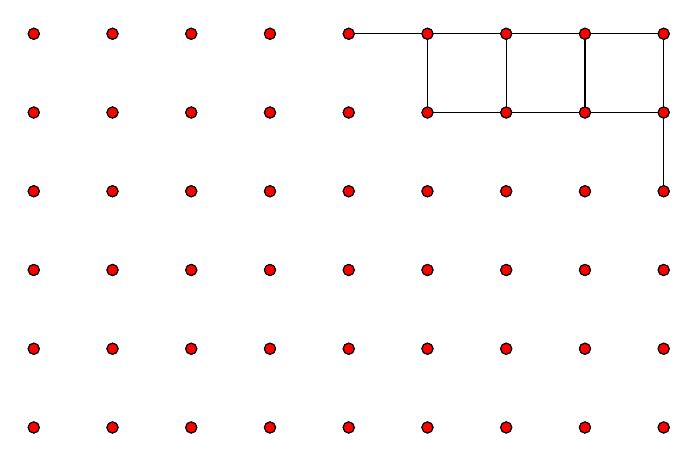
\begin{tikzpicture}[scale=1]%
\path[draw] (4.0,-7.0) -- (5.0,-7.0);%
\path[draw,radius=2pt] (4.0,-7.0) circle;%
\path[draw] (5.0,-7.0) -- (5.0,-8.0);%
\path[draw] (5.0,-7.0) -- (4.0,-7.0);%
\path[draw] (5.0,-7.0) -- (6.0,-7.0);%
\path[draw,radius=2pt] (5.0,-7.0) circle;%
\path[draw] (6.0,-7.0) -- (6.0,-8.0);%
\path[draw] (6.0,-7.0) -- (5.0,-7.0);%
\path[draw] (6.0,-7.0) -- (7.0,-7.0);%
\path[draw,radius=2pt] (6.0,-7.0) circle;%
\path[draw] (7.0,-7.0) -- (7.0,-8.0);%
\path[draw] (7.0,-7.0) -- (6.0,-7.0);%
\path[draw] (7.0,-7.0) -- (8.0,-7.0);%
\path[draw,radius=2pt] (7.0,-7.0) circle;%
\path[draw] (8.0,-7.0) -- (8.0,-8.0);%
\path[draw] (8.0,-7.0) -- (7.0,-7.0);%
\path[draw,radius=2pt] (8.0,-7.0) circle;%
\path[draw] (5.0,-8.0) -- (5.0,-7.0);%
\path[draw] (5.0,-8.0) -- (6.0,-8.0);%
\path[draw,radius=2pt] (5.0,-8.0) circle;%
\path[draw] (6.0,-8.0) -- (6.0,-7.0);%
\path[draw] (6.0,-8.0) -- (5.0,-8.0);%
\path[draw] (6.0,-8.0) -- (7.0,-8.0);%
\path[draw,radius=2pt] (6.0,-8.0) circle;%
\path[draw] (7.0,-8.0) -- (7.0,-7.0);%
\path[draw] (7.0,-8.0) -- (6.0,-8.0);%
\path[draw] (7.0,-8.0) -- (8.0,-8.0);%
\path[draw,radius=2pt] (7.0,-8.0) circle;%
\path[draw] (8.0,-8.0) -- (8.0,-7.0);%
\path[draw] (8.0,-8.0) -- (8.0,-9.0);%
\path[draw] (8.0,-8.0) -- (7.0,-8.0);%
\path[draw,radius=2pt] (8.0,-8.0) circle;%
\path[draw] (8.0,-9.0) -- (8.0,-8.0);%
\path[draw,radius=2pt] (8.0,-9.0) circle;%
\path[draw,radius=2pt,fill=red] (0.0,-7.0) circle;%
\path[draw,radius=2pt,fill=red] (1.0,-7.0) circle;%
\path[draw,radius=2pt,fill=red] (2.0,-7.0) circle;%
\path[draw,radius=2pt,fill=red] (3.0,-7.0) circle;%
\path[draw,radius=2pt,fill=red] (4.0,-7.0) circle;%
\path[draw,radius=2pt,fill=red] (5.0,-7.0) circle;%
\path[draw,radius=2pt,fill=red] (6.0,-7.0) circle;%
\path[draw,radius=2pt,fill=red] (7.0,-7.0) circle;%
\path[draw,radius=2pt,fill=red] (8.0,-7.0) circle;%
\path[draw,radius=2pt,fill=red] (0.0,-8.0) circle;%
\path[draw,radius=2pt,fill=red] (1.0,-8.0) circle;%
\path[draw,radius=2pt,fill=red] (2.0,-8.0) circle;%
\path[draw,radius=2pt,fill=red] (3.0,-8.0) circle;%
\path[draw,radius=2pt,fill=red] (4.0,-8.0) circle;%
\path[draw,radius=2pt,fill=red] (5.0,-8.0) circle;%
\path[draw,radius=2pt,fill=red] (6.0,-8.0) circle;%
\path[draw,radius=2pt,fill=red] (7.0,-8.0) circle;%
\path[draw,radius=2pt,fill=red] (8.0,-8.0) circle;%
\path[draw,radius=2pt,fill=red] (0.0,-9.0) circle;%
\path[draw,radius=2pt,fill=red] (1.0,-9.0) circle;%
\path[draw,radius=2pt,fill=red] (2.0,-9.0) circle;%
\path[draw,radius=2pt,fill=red] (3.0,-9.0) circle;%
\path[draw,radius=2pt,fill=red] (4.0,-9.0) circle;%
\path[draw,radius=2pt,fill=red] (5.0,-9.0) circle;%
\path[draw,radius=2pt,fill=red] (6.0,-9.0) circle;%
\path[draw,radius=2pt,fill=red] (7.0,-9.0) circle;%
\path[draw,radius=2pt,fill=red] (8.0,-9.0) circle;%
\path[draw,radius=2pt,fill=red] (0.0,-10.0) circle;%
\path[draw,radius=2pt,fill=red] (1.0,-10.0) circle;%
\path[draw,radius=2pt,fill=red] (2.0,-10.0) circle;%
\path[draw,radius=2pt,fill=red] (3.0,-10.0) circle;%
\path[draw,radius=2pt,fill=red] (4.0,-10.0) circle;%
\path[draw,radius=2pt,fill=red] (5.0,-10.0) circle;%
\path[draw,radius=2pt,fill=red] (6.0,-10.0) circle;%
\path[draw,radius=2pt,fill=red] (7.0,-10.0) circle;%
\path[draw,radius=2pt,fill=red] (8.0,-10.0) circle;%
\path[draw,radius=2pt,fill=red] (0.0,-11.0) circle;%
\path[draw,radius=2pt,fill=red] (1.0,-11.0) circle;%
\path[draw,radius=2pt,fill=red] (2.0,-11.0) circle;%
\path[draw,radius=2pt,fill=red] (3.0,-11.0) circle;%
\path[draw,radius=2pt,fill=red] (4.0,-11.0) circle;%
\path[draw,radius=2pt,fill=red] (5.0,-11.0) circle;%
\path[draw,radius=2pt,fill=red] (6.0,-11.0) circle;%
\path[draw,radius=2pt,fill=red] (7.0,-11.0) circle;%
\path[draw,radius=2pt,fill=red] (8.0,-11.0) circle;%
\path[draw,radius=2pt,fill=red] (0.0,-12.0) circle;%
\path[draw,radius=2pt,fill=red] (1.0,-12.0) circle;%
\path[draw,radius=2pt,fill=red] (2.0,-12.0) circle;%
\path[draw,radius=2pt,fill=red] (3.0,-12.0) circle;%
\path[draw,radius=2pt,fill=red] (4.0,-12.0) circle;%
\path[draw,radius=2pt,fill=red] (5.0,-12.0) circle;%
\path[draw,radius=2pt,fill=red] (6.0,-12.0) circle;%
\path[draw,radius=2pt,fill=red] (7.0,-12.0) circle;%
\path[draw,radius=2pt,fill=red] (8.0,-12.0) circle;%
\path[draw,radius=2pt,fill=red] (0.0,-7.0) circle;%
\path[draw,radius=2pt,fill=red] (1.0,-7.0) circle;%
\path[draw,radius=2pt,fill=red] (2.0,-7.0) circle;%
\path[draw,radius=2pt,fill=red] (3.0,-7.0) circle;%
\path[draw,radius=2pt,fill=red] (0.0,-8.0) circle;%
\path[draw,radius=2pt,fill=red] (1.0,-8.0) circle;%
\path[draw,radius=2pt,fill=red] (2.0,-8.0) circle;%
\path[draw,radius=2pt,fill=red] (3.0,-8.0) circle;%
\path[draw,radius=2pt,fill=red] (4.0,-8.0) circle;%
\path[draw,radius=2pt,fill=red] (0.0,-9.0) circle;%
\path[draw,radius=2pt,fill=red] (1.0,-9.0) circle;%
\path[draw,radius=2pt,fill=red] (2.0,-9.0) circle;%
\path[draw,radius=2pt,fill=red] (3.0,-9.0) circle;%
\path[draw,radius=2pt,fill=red] (4.0,-9.0) circle;%
\path[draw,radius=2pt,fill=red] (5.0,-9.0) circle;%
\path[draw,radius=2pt,fill=red] (6.0,-9.0) circle;%
\path[draw,radius=2pt,fill=red] (7.0,-9.0) circle;%
\path[draw,radius=2pt,fill=red] (0.0,-10.0) circle;%
\path[draw,radius=2pt,fill=red] (1.0,-10.0) circle;%
\path[draw,radius=2pt,fill=red] (2.0,-10.0) circle;%
\path[draw,radius=2pt,fill=red] (3.0,-10.0) circle;%
\path[draw,radius=2pt,fill=red] (4.0,-10.0) circle;%
\path[draw,radius=2pt,fill=red] (5.0,-10.0) circle;%
\path[draw,radius=2pt,fill=red] (6.0,-10.0) circle;%
\path[draw,radius=2pt,fill=red] (7.0,-10.0) circle;%
\path[draw,radius=2pt,fill=red] (8.0,-10.0) circle;%
\path[draw,radius=2pt,fill=red] (0.0,-11.0) circle;%
\path[draw,radius=2pt,fill=red] (1.0,-11.0) circle;%
\path[draw,radius=2pt,fill=red] (2.0,-11.0) circle;%
\path[draw,radius=2pt,fill=red] (3.0,-11.0) circle;%
\path[draw,radius=2pt,fill=red] (4.0,-11.0) circle;%
\path[draw,radius=2pt,fill=red] (5.0,-11.0) circle;%
\path[draw,radius=2pt,fill=red] (6.0,-11.0) circle;%
\path[draw,radius=2pt,fill=red] (7.0,-11.0) circle;%
\path[draw,radius=2pt,fill=red] (8.0,-11.0) circle;%
\path[draw,radius=2pt,fill=red] (0.0,-12.0) circle;%
\path[draw,radius=2pt,fill=red] (1.0,-12.0) circle;%
\path[draw,radius=2pt,fill=red] (2.0,-12.0) circle;%
\path[draw,radius=2pt,fill=red] (3.0,-12.0) circle;%
\path[draw,radius=2pt,fill=red] (4.0,-12.0) circle;%
\path[draw,radius=2pt,fill=red] (5.0,-12.0) circle;%
\path[draw,radius=2pt,fill=red] (6.0,-12.0) circle;%
\path[draw,radius=2pt,fill=red] (7.0,-12.0) circle;%
\path[draw,radius=2pt,fill=red] (8.0,-12.0) circle;%
\end{tikzpicture}%
\newline%
\hspace*{1in}%
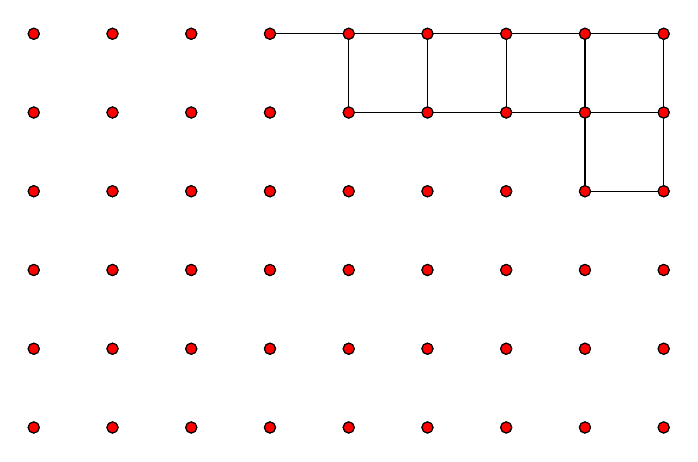
\begin{tikzpicture}[scale=1]%
\path[draw] (3.0,-7.0) -- (4.0,-7.0);%
\path[draw,radius=2pt] (3.0,-7.0) circle;%
\path[draw] (4.0,-7.0) -- (4.0,-8.0);%
\path[draw] (4.0,-7.0) -- (3.0,-7.0);%
\path[draw] (4.0,-7.0) -- (5.0,-7.0);%
\path[draw,radius=2pt] (4.0,-7.0) circle;%
\path[draw] (5.0,-7.0) -- (5.0,-8.0);%
\path[draw] (5.0,-7.0) -- (4.0,-7.0);%
\path[draw] (5.0,-7.0) -- (6.0,-7.0);%
\path[draw,radius=2pt] (5.0,-7.0) circle;%
\path[draw] (6.0,-7.0) -- (6.0,-8.0);%
\path[draw] (6.0,-7.0) -- (5.0,-7.0);%
\path[draw] (6.0,-7.0) -- (7.0,-7.0);%
\path[draw,radius=2pt] (6.0,-7.0) circle;%
\path[draw] (7.0,-7.0) -- (7.0,-8.0);%
\path[draw] (7.0,-7.0) -- (6.0,-7.0);%
\path[draw] (7.0,-7.0) -- (8.0,-7.0);%
\path[draw,radius=2pt] (7.0,-7.0) circle;%
\path[draw] (8.0,-7.0) -- (8.0,-8.0);%
\path[draw] (8.0,-7.0) -- (7.0,-7.0);%
\path[draw,radius=2pt] (8.0,-7.0) circle;%
\path[draw] (4.0,-8.0) -- (4.0,-7.0);%
\path[draw] (4.0,-8.0) -- (5.0,-8.0);%
\path[draw,radius=2pt] (4.0,-8.0) circle;%
\path[draw] (5.0,-8.0) -- (5.0,-7.0);%
\path[draw] (5.0,-8.0) -- (4.0,-8.0);%
\path[draw] (5.0,-8.0) -- (6.0,-8.0);%
\path[draw,radius=2pt] (5.0,-8.0) circle;%
\path[draw] (6.0,-8.0) -- (6.0,-7.0);%
\path[draw] (6.0,-8.0) -- (5.0,-8.0);%
\path[draw] (6.0,-8.0) -- (7.0,-8.0);%
\path[draw,radius=2pt] (6.0,-8.0) circle;%
\path[draw] (7.0,-8.0) -- (7.0,-7.0);%
\path[draw] (7.0,-8.0) -- (7.0,-9.0);%
\path[draw] (7.0,-8.0) -- (6.0,-8.0);%
\path[draw] (7.0,-8.0) -- (8.0,-8.0);%
\path[draw,radius=2pt] (7.0,-8.0) circle;%
\path[draw] (8.0,-8.0) -- (8.0,-7.0);%
\path[draw] (8.0,-8.0) -- (8.0,-9.0);%
\path[draw] (8.0,-8.0) -- (7.0,-8.0);%
\path[draw,radius=2pt] (8.0,-8.0) circle;%
\path[draw] (7.0,-9.0) -- (7.0,-8.0);%
\path[draw] (7.0,-9.0) -- (8.0,-9.0);%
\path[draw,radius=2pt] (7.0,-9.0) circle;%
\path[draw] (8.0,-9.0) -- (8.0,-8.0);%
\path[draw] (8.0,-9.0) -- (7.0,-9.0);%
\path[draw,radius=2pt] (8.0,-9.0) circle;%
\path[draw,radius=2pt,fill=red] (0.0,-7.0) circle;%
\path[draw,radius=2pt,fill=red] (1.0,-7.0) circle;%
\path[draw,radius=2pt,fill=red] (2.0,-7.0) circle;%
\path[draw,radius=2pt,fill=red] (3.0,-7.0) circle;%
\path[draw,radius=2pt,fill=red] (4.0,-7.0) circle;%
\path[draw,radius=2pt,fill=red] (5.0,-7.0) circle;%
\path[draw,radius=2pt,fill=red] (6.0,-7.0) circle;%
\path[draw,radius=2pt,fill=red] (7.0,-7.0) circle;%
\path[draw,radius=2pt,fill=red] (8.0,-7.0) circle;%
\path[draw,radius=2pt,fill=red] (0.0,-8.0) circle;%
\path[draw,radius=2pt,fill=red] (1.0,-8.0) circle;%
\path[draw,radius=2pt,fill=red] (2.0,-8.0) circle;%
\path[draw,radius=2pt,fill=red] (3.0,-8.0) circle;%
\path[draw,radius=2pt,fill=red] (4.0,-8.0) circle;%
\path[draw,radius=2pt,fill=red] (5.0,-8.0) circle;%
\path[draw,radius=2pt,fill=red] (6.0,-8.0) circle;%
\path[draw,radius=2pt,fill=red] (7.0,-8.0) circle;%
\path[draw,radius=2pt,fill=red] (8.0,-8.0) circle;%
\path[draw,radius=2pt,fill=red] (0.0,-9.0) circle;%
\path[draw,radius=2pt,fill=red] (1.0,-9.0) circle;%
\path[draw,radius=2pt,fill=red] (2.0,-9.0) circle;%
\path[draw,radius=2pt,fill=red] (3.0,-9.0) circle;%
\path[draw,radius=2pt,fill=red] (4.0,-9.0) circle;%
\path[draw,radius=2pt,fill=red] (5.0,-9.0) circle;%
\path[draw,radius=2pt,fill=red] (6.0,-9.0) circle;%
\path[draw,radius=2pt,fill=red] (7.0,-9.0) circle;%
\path[draw,radius=2pt,fill=red] (8.0,-9.0) circle;%
\path[draw,radius=2pt,fill=red] (0.0,-10.0) circle;%
\path[draw,radius=2pt,fill=red] (1.0,-10.0) circle;%
\path[draw,radius=2pt,fill=red] (2.0,-10.0) circle;%
\path[draw,radius=2pt,fill=red] (3.0,-10.0) circle;%
\path[draw,radius=2pt,fill=red] (4.0,-10.0) circle;%
\path[draw,radius=2pt,fill=red] (5.0,-10.0) circle;%
\path[draw,radius=2pt,fill=red] (6.0,-10.0) circle;%
\path[draw,radius=2pt,fill=red] (7.0,-10.0) circle;%
\path[draw,radius=2pt,fill=red] (8.0,-10.0) circle;%
\path[draw,radius=2pt,fill=red] (0.0,-11.0) circle;%
\path[draw,radius=2pt,fill=red] (1.0,-11.0) circle;%
\path[draw,radius=2pt,fill=red] (2.0,-11.0) circle;%
\path[draw,radius=2pt,fill=red] (3.0,-11.0) circle;%
\path[draw,radius=2pt,fill=red] (4.0,-11.0) circle;%
\path[draw,radius=2pt,fill=red] (5.0,-11.0) circle;%
\path[draw,radius=2pt,fill=red] (6.0,-11.0) circle;%
\path[draw,radius=2pt,fill=red] (7.0,-11.0) circle;%
\path[draw,radius=2pt,fill=red] (8.0,-11.0) circle;%
\path[draw,radius=2pt,fill=red] (0.0,-12.0) circle;%
\path[draw,radius=2pt,fill=red] (1.0,-12.0) circle;%
\path[draw,radius=2pt,fill=red] (2.0,-12.0) circle;%
\path[draw,radius=2pt,fill=red] (3.0,-12.0) circle;%
\path[draw,radius=2pt,fill=red] (4.0,-12.0) circle;%
\path[draw,radius=2pt,fill=red] (5.0,-12.0) circle;%
\path[draw,radius=2pt,fill=red] (6.0,-12.0) circle;%
\path[draw,radius=2pt,fill=red] (7.0,-12.0) circle;%
\path[draw,radius=2pt,fill=red] (8.0,-12.0) circle;%
\path[draw,radius=2pt,fill=red] (0.0,-7.0) circle;%
\path[draw,radius=2pt,fill=red] (1.0,-7.0) circle;%
\path[draw,radius=2pt,fill=red] (2.0,-7.0) circle;%
\path[draw,radius=2pt,fill=red] (0.0,-8.0) circle;%
\path[draw,radius=2pt,fill=red] (1.0,-8.0) circle;%
\path[draw,radius=2pt,fill=red] (2.0,-8.0) circle;%
\path[draw,radius=2pt,fill=red] (3.0,-8.0) circle;%
\path[draw,radius=2pt,fill=red] (0.0,-9.0) circle;%
\path[draw,radius=2pt,fill=red] (1.0,-9.0) circle;%
\path[draw,radius=2pt,fill=red] (2.0,-9.0) circle;%
\path[draw,radius=2pt,fill=red] (3.0,-9.0) circle;%
\path[draw,radius=2pt,fill=red] (4.0,-9.0) circle;%
\path[draw,radius=2pt,fill=red] (5.0,-9.0) circle;%
\path[draw,radius=2pt,fill=red] (6.0,-9.0) circle;%
\path[draw,radius=2pt,fill=red] (0.0,-10.0) circle;%
\path[draw,radius=2pt,fill=red] (1.0,-10.0) circle;%
\path[draw,radius=2pt,fill=red] (2.0,-10.0) circle;%
\path[draw,radius=2pt,fill=red] (3.0,-10.0) circle;%
\path[draw,radius=2pt,fill=red] (4.0,-10.0) circle;%
\path[draw,radius=2pt,fill=red] (5.0,-10.0) circle;%
\path[draw,radius=2pt,fill=red] (6.0,-10.0) circle;%
\path[draw,radius=2pt,fill=red] (7.0,-10.0) circle;%
\path[draw,radius=2pt,fill=red] (8.0,-10.0) circle;%
\path[draw,radius=2pt,fill=red] (0.0,-11.0) circle;%
\path[draw,radius=2pt,fill=red] (1.0,-11.0) circle;%
\path[draw,radius=2pt,fill=red] (2.0,-11.0) circle;%
\path[draw,radius=2pt,fill=red] (3.0,-11.0) circle;%
\path[draw,radius=2pt,fill=red] (4.0,-11.0) circle;%
\path[draw,radius=2pt,fill=red] (5.0,-11.0) circle;%
\path[draw,radius=2pt,fill=red] (6.0,-11.0) circle;%
\path[draw,radius=2pt,fill=red] (7.0,-11.0) circle;%
\path[draw,radius=2pt,fill=red] (8.0,-11.0) circle;%
\path[draw,radius=2pt,fill=red] (0.0,-12.0) circle;%
\path[draw,radius=2pt,fill=red] (1.0,-12.0) circle;%
\path[draw,radius=2pt,fill=red] (2.0,-12.0) circle;%
\path[draw,radius=2pt,fill=red] (3.0,-12.0) circle;%
\path[draw,radius=2pt,fill=red] (4.0,-12.0) circle;%
\path[draw,radius=2pt,fill=red] (5.0,-12.0) circle;%
\path[draw,radius=2pt,fill=red] (6.0,-12.0) circle;%
\path[draw,radius=2pt,fill=red] (7.0,-12.0) circle;%
\path[draw,radius=2pt,fill=red] (8.0,-12.0) circle;%
\end{tikzpicture}%
\hspace*{1in}%
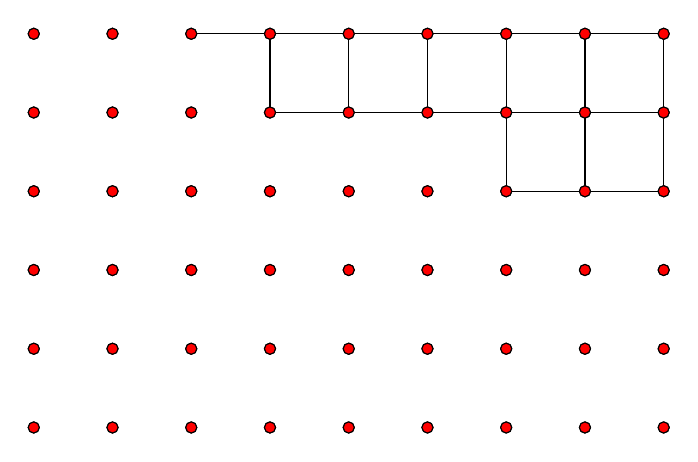
\begin{tikzpicture}[scale=1]%
\path[draw,radius=2pt] (0.0,-7.0) circle;%
\path[draw] (2.0,-7.0) -- (3.0,-7.0);%
\path[draw,radius=2pt] (2.0,-7.0) circle;%
\path[draw] (3.0,-7.0) -- (3.0,-8.0);%
\path[draw] (3.0,-7.0) -- (2.0,-7.0);%
\path[draw] (3.0,-7.0) -- (4.0,-7.0);%
\path[draw,radius=2pt] (3.0,-7.0) circle;%
\path[draw] (4.0,-7.0) -- (4.0,-8.0);%
\path[draw] (4.0,-7.0) -- (3.0,-7.0);%
\path[draw] (4.0,-7.0) -- (5.0,-7.0);%
\path[draw,radius=2pt] (4.0,-7.0) circle;%
\path[draw] (5.0,-7.0) -- (5.0,-8.0);%
\path[draw] (5.0,-7.0) -- (4.0,-7.0);%
\path[draw] (5.0,-7.0) -- (6.0,-7.0);%
\path[draw,radius=2pt] (5.0,-7.0) circle;%
\path[draw] (6.0,-7.0) -- (6.0,-8.0);%
\path[draw] (6.0,-7.0) -- (5.0,-7.0);%
\path[draw] (6.0,-7.0) -- (7.0,-7.0);%
\path[draw,radius=2pt] (6.0,-7.0) circle;%
\path[draw] (7.0,-7.0) -- (7.0,-8.0);%
\path[draw] (7.0,-7.0) -- (6.0,-7.0);%
\path[draw] (7.0,-7.0) -- (8.0,-7.0);%
\path[draw,radius=2pt] (7.0,-7.0) circle;%
\path[draw] (8.0,-7.0) -- (8.0,-8.0);%
\path[draw] (8.0,-7.0) -- (7.0,-7.0);%
\path[draw,radius=2pt] (8.0,-7.0) circle;%
\path[draw] (3.0,-8.0) -- (3.0,-7.0);%
\path[draw] (3.0,-8.0) -- (4.0,-8.0);%
\path[draw,radius=2pt] (3.0,-8.0) circle;%
\path[draw] (4.0,-8.0) -- (4.0,-7.0);%
\path[draw] (4.0,-8.0) -- (3.0,-8.0);%
\path[draw] (4.0,-8.0) -- (5.0,-8.0);%
\path[draw,radius=2pt] (4.0,-8.0) circle;%
\path[draw] (5.0,-8.0) -- (5.0,-7.0);%
\path[draw] (5.0,-8.0) -- (4.0,-8.0);%
\path[draw] (5.0,-8.0) -- (6.0,-8.0);%
\path[draw,radius=2pt] (5.0,-8.0) circle;%
\path[draw] (6.0,-8.0) -- (6.0,-7.0);%
\path[draw] (6.0,-8.0) -- (6.0,-9.0);%
\path[draw] (6.0,-8.0) -- (5.0,-8.0);%
\path[draw] (6.0,-8.0) -- (7.0,-8.0);%
\path[draw,radius=2pt] (6.0,-8.0) circle;%
\path[draw] (7.0,-8.0) -- (7.0,-7.0);%
\path[draw] (7.0,-8.0) -- (7.0,-9.0);%
\path[draw] (7.0,-8.0) -- (6.0,-8.0);%
\path[draw] (7.0,-8.0) -- (8.0,-8.0);%
\path[draw,radius=2pt] (7.0,-8.0) circle;%
\path[draw] (8.0,-8.0) -- (8.0,-7.0);%
\path[draw] (8.0,-8.0) -- (8.0,-9.0);%
\path[draw] (8.0,-8.0) -- (7.0,-8.0);%
\path[draw,radius=2pt] (8.0,-8.0) circle;%
\path[draw] (6.0,-9.0) -- (6.0,-8.0);%
\path[draw] (6.0,-9.0) -- (7.0,-9.0);%
\path[draw,radius=2pt] (6.0,-9.0) circle;%
\path[draw] (7.0,-9.0) -- (7.0,-8.0);%
\path[draw] (7.0,-9.0) -- (6.0,-9.0);%
\path[draw] (7.0,-9.0) -- (8.0,-9.0);%
\path[draw,radius=2pt] (7.0,-9.0) circle;%
\path[draw] (8.0,-9.0) -- (8.0,-8.0);%
\path[draw] (8.0,-9.0) -- (7.0,-9.0);%
\path[draw,radius=2pt] (8.0,-9.0) circle;%
\path[draw,radius=2pt,fill=red] (0.0,-7.0) circle;%
\path[draw,radius=2pt,fill=red] (1.0,-7.0) circle;%
\path[draw,radius=2pt,fill=red] (2.0,-7.0) circle;%
\path[draw,radius=2pt,fill=red] (3.0,-7.0) circle;%
\path[draw,radius=2pt,fill=red] (4.0,-7.0) circle;%
\path[draw,radius=2pt,fill=red] (5.0,-7.0) circle;%
\path[draw,radius=2pt,fill=red] (6.0,-7.0) circle;%
\path[draw,radius=2pt,fill=red] (7.0,-7.0) circle;%
\path[draw,radius=2pt,fill=red] (8.0,-7.0) circle;%
\path[draw,radius=2pt,fill=red] (0.0,-8.0) circle;%
\path[draw,radius=2pt,fill=red] (1.0,-8.0) circle;%
\path[draw,radius=2pt,fill=red] (2.0,-8.0) circle;%
\path[draw,radius=2pt,fill=red] (3.0,-8.0) circle;%
\path[draw,radius=2pt,fill=red] (4.0,-8.0) circle;%
\path[draw,radius=2pt,fill=red] (5.0,-8.0) circle;%
\path[draw,radius=2pt,fill=red] (6.0,-8.0) circle;%
\path[draw,radius=2pt,fill=red] (7.0,-8.0) circle;%
\path[draw,radius=2pt,fill=red] (8.0,-8.0) circle;%
\path[draw,radius=2pt,fill=red] (0.0,-9.0) circle;%
\path[draw,radius=2pt,fill=red] (1.0,-9.0) circle;%
\path[draw,radius=2pt,fill=red] (2.0,-9.0) circle;%
\path[draw,radius=2pt,fill=red] (3.0,-9.0) circle;%
\path[draw,radius=2pt,fill=red] (4.0,-9.0) circle;%
\path[draw,radius=2pt,fill=red] (5.0,-9.0) circle;%
\path[draw,radius=2pt,fill=red] (6.0,-9.0) circle;%
\path[draw,radius=2pt,fill=red] (7.0,-9.0) circle;%
\path[draw,radius=2pt,fill=red] (8.0,-9.0) circle;%
\path[draw,radius=2pt,fill=red] (0.0,-10.0) circle;%
\path[draw,radius=2pt,fill=red] (1.0,-10.0) circle;%
\path[draw,radius=2pt,fill=red] (2.0,-10.0) circle;%
\path[draw,radius=2pt,fill=red] (3.0,-10.0) circle;%
\path[draw,radius=2pt,fill=red] (4.0,-10.0) circle;%
\path[draw,radius=2pt,fill=red] (5.0,-10.0) circle;%
\path[draw,radius=2pt,fill=red] (6.0,-10.0) circle;%
\path[draw,radius=2pt,fill=red] (7.0,-10.0) circle;%
\path[draw,radius=2pt,fill=red] (8.0,-10.0) circle;%
\path[draw,radius=2pt,fill=red] (0.0,-11.0) circle;%
\path[draw,radius=2pt,fill=red] (1.0,-11.0) circle;%
\path[draw,radius=2pt,fill=red] (2.0,-11.0) circle;%
\path[draw,radius=2pt,fill=red] (3.0,-11.0) circle;%
\path[draw,radius=2pt,fill=red] (4.0,-11.0) circle;%
\path[draw,radius=2pt,fill=red] (5.0,-11.0) circle;%
\path[draw,radius=2pt,fill=red] (6.0,-11.0) circle;%
\path[draw,radius=2pt,fill=red] (7.0,-11.0) circle;%
\path[draw,radius=2pt,fill=red] (8.0,-11.0) circle;%
\path[draw,radius=2pt,fill=red] (0.0,-12.0) circle;%
\path[draw,radius=2pt,fill=red] (1.0,-12.0) circle;%
\path[draw,radius=2pt,fill=red] (2.0,-12.0) circle;%
\path[draw,radius=2pt,fill=red] (3.0,-12.0) circle;%
\path[draw,radius=2pt,fill=red] (4.0,-12.0) circle;%
\path[draw,radius=2pt,fill=red] (5.0,-12.0) circle;%
\path[draw,radius=2pt,fill=red] (6.0,-12.0) circle;%
\path[draw,radius=2pt,fill=red] (7.0,-12.0) circle;%
\path[draw,radius=2pt,fill=red] (8.0,-12.0) circle;%
\path[draw,radius=2pt,fill=red] (1.0,-7.0) circle;%
\path[draw,radius=2pt,fill=red] (0.0,-8.0) circle;%
\path[draw,radius=2pt,fill=red] (1.0,-8.0) circle;%
\path[draw,radius=2pt,fill=red] (2.0,-8.0) circle;%
\path[draw,radius=2pt,fill=red] (0.0,-9.0) circle;%
\path[draw,radius=2pt,fill=red] (1.0,-9.0) circle;%
\path[draw,radius=2pt,fill=red] (2.0,-9.0) circle;%
\path[draw,radius=2pt,fill=red] (3.0,-9.0) circle;%
\path[draw,radius=2pt,fill=red] (4.0,-9.0) circle;%
\path[draw,radius=2pt,fill=red] (5.0,-9.0) circle;%
\path[draw,radius=2pt,fill=red] (0.0,-10.0) circle;%
\path[draw,radius=2pt,fill=red] (1.0,-10.0) circle;%
\path[draw,radius=2pt,fill=red] (2.0,-10.0) circle;%
\path[draw,radius=2pt,fill=red] (3.0,-10.0) circle;%
\path[draw,radius=2pt,fill=red] (4.0,-10.0) circle;%
\path[draw,radius=2pt,fill=red] (5.0,-10.0) circle;%
\path[draw,radius=2pt,fill=red] (6.0,-10.0) circle;%
\path[draw,radius=2pt,fill=red] (7.0,-10.0) circle;%
\path[draw,radius=2pt,fill=red] (8.0,-10.0) circle;%
\path[draw,radius=2pt,fill=red] (0.0,-11.0) circle;%
\path[draw,radius=2pt,fill=red] (1.0,-11.0) circle;%
\path[draw,radius=2pt,fill=red] (2.0,-11.0) circle;%
\path[draw,radius=2pt,fill=red] (3.0,-11.0) circle;%
\path[draw,radius=2pt,fill=red] (4.0,-11.0) circle;%
\path[draw,radius=2pt,fill=red] (5.0,-11.0) circle;%
\path[draw,radius=2pt,fill=red] (6.0,-11.0) circle;%
\path[draw,radius=2pt,fill=red] (7.0,-11.0) circle;%
\path[draw,radius=2pt,fill=red] (8.0,-11.0) circle;%
\path[draw,radius=2pt,fill=red] (0.0,-12.0) circle;%
\path[draw,radius=2pt,fill=red] (1.0,-12.0) circle;%
\path[draw,radius=2pt,fill=red] (2.0,-12.0) circle;%
\path[draw,radius=2pt,fill=red] (3.0,-12.0) circle;%
\path[draw,radius=2pt,fill=red] (4.0,-12.0) circle;%
\path[draw,radius=2pt,fill=red] (5.0,-12.0) circle;%
\path[draw,radius=2pt,fill=red] (6.0,-12.0) circle;%
\path[draw,radius=2pt,fill=red] (7.0,-12.0) circle;%
\path[draw,radius=2pt,fill=red] (8.0,-12.0) circle;%
\end{tikzpicture}%
\hspace*{1in}%
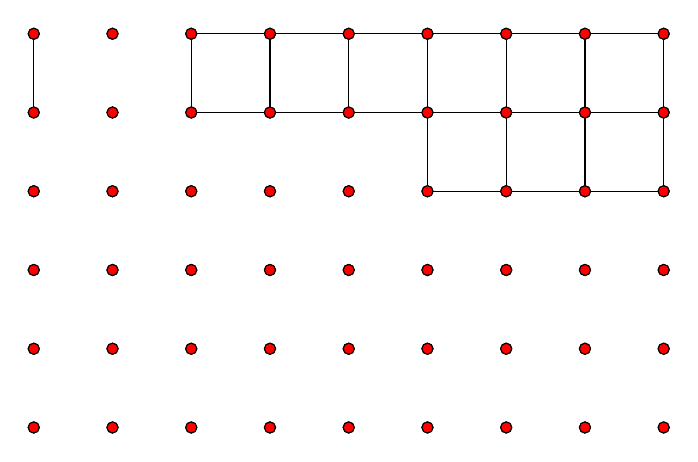
\begin{tikzpicture}[scale=1]%
\path[draw] (0.0,-7.0) -- (0.0,-8.0);%
\path[draw,radius=2pt] (0.0,-7.0) circle;%
\path[draw] (2.0,-7.0) -- (2.0,-8.0);%
\path[draw] (2.0,-7.0) -- (3.0,-7.0);%
\path[draw,radius=2pt] (2.0,-7.0) circle;%
\path[draw] (3.0,-7.0) -- (3.0,-8.0);%
\path[draw] (3.0,-7.0) -- (2.0,-7.0);%
\path[draw] (3.0,-7.0) -- (4.0,-7.0);%
\path[draw,radius=2pt] (3.0,-7.0) circle;%
\path[draw] (4.0,-7.0) -- (4.0,-8.0);%
\path[draw] (4.0,-7.0) -- (3.0,-7.0);%
\path[draw] (4.0,-7.0) -- (5.0,-7.0);%
\path[draw,radius=2pt] (4.0,-7.0) circle;%
\path[draw] (5.0,-7.0) -- (5.0,-8.0);%
\path[draw] (5.0,-7.0) -- (4.0,-7.0);%
\path[draw] (5.0,-7.0) -- (6.0,-7.0);%
\path[draw,radius=2pt] (5.0,-7.0) circle;%
\path[draw] (6.0,-7.0) -- (6.0,-8.0);%
\path[draw] (6.0,-7.0) -- (5.0,-7.0);%
\path[draw] (6.0,-7.0) -- (7.0,-7.0);%
\path[draw,radius=2pt] (6.0,-7.0) circle;%
\path[draw] (7.0,-7.0) -- (7.0,-8.0);%
\path[draw] (7.0,-7.0) -- (6.0,-7.0);%
\path[draw] (7.0,-7.0) -- (8.0,-7.0);%
\path[draw,radius=2pt] (7.0,-7.0) circle;%
\path[draw] (8.0,-7.0) -- (8.0,-8.0);%
\path[draw] (8.0,-7.0) -- (7.0,-7.0);%
\path[draw,radius=2pt] (8.0,-7.0) circle;%
\path[draw] (0.0,-8.0) -- (0.0,-7.0);%
\path[draw,radius=2pt] (0.0,-8.0) circle;%
\path[draw] (2.0,-8.0) -- (2.0,-7.0);%
\path[draw] (2.0,-8.0) -- (3.0,-8.0);%
\path[draw,radius=2pt] (2.0,-8.0) circle;%
\path[draw] (3.0,-8.0) -- (3.0,-7.0);%
\path[draw] (3.0,-8.0) -- (2.0,-8.0);%
\path[draw] (3.0,-8.0) -- (4.0,-8.0);%
\path[draw,radius=2pt] (3.0,-8.0) circle;%
\path[draw] (4.0,-8.0) -- (4.0,-7.0);%
\path[draw] (4.0,-8.0) -- (3.0,-8.0);%
\path[draw] (4.0,-8.0) -- (5.0,-8.0);%
\path[draw,radius=2pt] (4.0,-8.0) circle;%
\path[draw] (5.0,-8.0) -- (5.0,-7.0);%
\path[draw] (5.0,-8.0) -- (5.0,-9.0);%
\path[draw] (5.0,-8.0) -- (4.0,-8.0);%
\path[draw] (5.0,-8.0) -- (6.0,-8.0);%
\path[draw,radius=2pt] (5.0,-8.0) circle;%
\path[draw] (6.0,-8.0) -- (6.0,-7.0);%
\path[draw] (6.0,-8.0) -- (6.0,-9.0);%
\path[draw] (6.0,-8.0) -- (5.0,-8.0);%
\path[draw] (6.0,-8.0) -- (7.0,-8.0);%
\path[draw,radius=2pt] (6.0,-8.0) circle;%
\path[draw] (7.0,-8.0) -- (7.0,-7.0);%
\path[draw] (7.0,-8.0) -- (7.0,-9.0);%
\path[draw] (7.0,-8.0) -- (6.0,-8.0);%
\path[draw] (7.0,-8.0) -- (8.0,-8.0);%
\path[draw,radius=2pt] (7.0,-8.0) circle;%
\path[draw] (8.0,-8.0) -- (8.0,-7.0);%
\path[draw] (8.0,-8.0) -- (8.0,-9.0);%
\path[draw] (8.0,-8.0) -- (7.0,-8.0);%
\path[draw,radius=2pt] (8.0,-8.0) circle;%
\path[draw] (5.0,-9.0) -- (5.0,-8.0);%
\path[draw] (5.0,-9.0) -- (6.0,-9.0);%
\path[draw,radius=2pt] (5.0,-9.0) circle;%
\path[draw] (6.0,-9.0) -- (6.0,-8.0);%
\path[draw] (6.0,-9.0) -- (5.0,-9.0);%
\path[draw] (6.0,-9.0) -- (7.0,-9.0);%
\path[draw,radius=2pt] (6.0,-9.0) circle;%
\path[draw] (7.0,-9.0) -- (7.0,-8.0);%
\path[draw] (7.0,-9.0) -- (6.0,-9.0);%
\path[draw] (7.0,-9.0) -- (8.0,-9.0);%
\path[draw,radius=2pt] (7.0,-9.0) circle;%
\path[draw] (8.0,-9.0) -- (8.0,-8.0);%
\path[draw] (8.0,-9.0) -- (7.0,-9.0);%
\path[draw,radius=2pt] (8.0,-9.0) circle;%
\path[draw,radius=2pt,fill=red] (0.0,-7.0) circle;%
\path[draw,radius=2pt,fill=red] (1.0,-7.0) circle;%
\path[draw,radius=2pt,fill=red] (2.0,-7.0) circle;%
\path[draw,radius=2pt,fill=red] (3.0,-7.0) circle;%
\path[draw,radius=2pt,fill=red] (4.0,-7.0) circle;%
\path[draw,radius=2pt,fill=red] (5.0,-7.0) circle;%
\path[draw,radius=2pt,fill=red] (6.0,-7.0) circle;%
\path[draw,radius=2pt,fill=red] (7.0,-7.0) circle;%
\path[draw,radius=2pt,fill=red] (8.0,-7.0) circle;%
\path[draw,radius=2pt,fill=red] (0.0,-8.0) circle;%
\path[draw,radius=2pt,fill=red] (1.0,-8.0) circle;%
\path[draw,radius=2pt,fill=red] (2.0,-8.0) circle;%
\path[draw,radius=2pt,fill=red] (3.0,-8.0) circle;%
\path[draw,radius=2pt,fill=red] (4.0,-8.0) circle;%
\path[draw,radius=2pt,fill=red] (5.0,-8.0) circle;%
\path[draw,radius=2pt,fill=red] (6.0,-8.0) circle;%
\path[draw,radius=2pt,fill=red] (7.0,-8.0) circle;%
\path[draw,radius=2pt,fill=red] (8.0,-8.0) circle;%
\path[draw,radius=2pt,fill=red] (0.0,-9.0) circle;%
\path[draw,radius=2pt,fill=red] (1.0,-9.0) circle;%
\path[draw,radius=2pt,fill=red] (2.0,-9.0) circle;%
\path[draw,radius=2pt,fill=red] (3.0,-9.0) circle;%
\path[draw,radius=2pt,fill=red] (4.0,-9.0) circle;%
\path[draw,radius=2pt,fill=red] (5.0,-9.0) circle;%
\path[draw,radius=2pt,fill=red] (6.0,-9.0) circle;%
\path[draw,radius=2pt,fill=red] (7.0,-9.0) circle;%
\path[draw,radius=2pt,fill=red] (8.0,-9.0) circle;%
\path[draw,radius=2pt,fill=red] (0.0,-10.0) circle;%
\path[draw,radius=2pt,fill=red] (1.0,-10.0) circle;%
\path[draw,radius=2pt,fill=red] (2.0,-10.0) circle;%
\path[draw,radius=2pt,fill=red] (3.0,-10.0) circle;%
\path[draw,radius=2pt,fill=red] (4.0,-10.0) circle;%
\path[draw,radius=2pt,fill=red] (5.0,-10.0) circle;%
\path[draw,radius=2pt,fill=red] (6.0,-10.0) circle;%
\path[draw,radius=2pt,fill=red] (7.0,-10.0) circle;%
\path[draw,radius=2pt,fill=red] (8.0,-10.0) circle;%
\path[draw,radius=2pt,fill=red] (0.0,-11.0) circle;%
\path[draw,radius=2pt,fill=red] (1.0,-11.0) circle;%
\path[draw,radius=2pt,fill=red] (2.0,-11.0) circle;%
\path[draw,radius=2pt,fill=red] (3.0,-11.0) circle;%
\path[draw,radius=2pt,fill=red] (4.0,-11.0) circle;%
\path[draw,radius=2pt,fill=red] (5.0,-11.0) circle;%
\path[draw,radius=2pt,fill=red] (6.0,-11.0) circle;%
\path[draw,radius=2pt,fill=red] (7.0,-11.0) circle;%
\path[draw,radius=2pt,fill=red] (8.0,-11.0) circle;%
\path[draw,radius=2pt,fill=red] (0.0,-12.0) circle;%
\path[draw,radius=2pt,fill=red] (1.0,-12.0) circle;%
\path[draw,radius=2pt,fill=red] (2.0,-12.0) circle;%
\path[draw,radius=2pt,fill=red] (3.0,-12.0) circle;%
\path[draw,radius=2pt,fill=red] (4.0,-12.0) circle;%
\path[draw,radius=2pt,fill=red] (5.0,-12.0) circle;%
\path[draw,radius=2pt,fill=red] (6.0,-12.0) circle;%
\path[draw,radius=2pt,fill=red] (7.0,-12.0) circle;%
\path[draw,radius=2pt,fill=red] (8.0,-12.0) circle;%
\path[draw,radius=2pt,fill=red] (1.0,-7.0) circle;%
\path[draw,radius=2pt,fill=red] (1.0,-8.0) circle;%
\path[draw,radius=2pt,fill=red] (0.0,-9.0) circle;%
\path[draw,radius=2pt,fill=red] (1.0,-9.0) circle;%
\path[draw,radius=2pt,fill=red] (2.0,-9.0) circle;%
\path[draw,radius=2pt,fill=red] (3.0,-9.0) circle;%
\path[draw,radius=2pt,fill=red] (4.0,-9.0) circle;%
\path[draw,radius=2pt,fill=red] (0.0,-10.0) circle;%
\path[draw,radius=2pt,fill=red] (1.0,-10.0) circle;%
\path[draw,radius=2pt,fill=red] (2.0,-10.0) circle;%
\path[draw,radius=2pt,fill=red] (3.0,-10.0) circle;%
\path[draw,radius=2pt,fill=red] (4.0,-10.0) circle;%
\path[draw,radius=2pt,fill=red] (5.0,-10.0) circle;%
\path[draw,radius=2pt,fill=red] (6.0,-10.0) circle;%
\path[draw,radius=2pt,fill=red] (7.0,-10.0) circle;%
\path[draw,radius=2pt,fill=red] (8.0,-10.0) circle;%
\path[draw,radius=2pt,fill=red] (0.0,-11.0) circle;%
\path[draw,radius=2pt,fill=red] (1.0,-11.0) circle;%
\path[draw,radius=2pt,fill=red] (2.0,-11.0) circle;%
\path[draw,radius=2pt,fill=red] (3.0,-11.0) circle;%
\path[draw,radius=2pt,fill=red] (4.0,-11.0) circle;%
\path[draw,radius=2pt,fill=red] (5.0,-11.0) circle;%
\path[draw,radius=2pt,fill=red] (6.0,-11.0) circle;%
\path[draw,radius=2pt,fill=red] (7.0,-11.0) circle;%
\path[draw,radius=2pt,fill=red] (8.0,-11.0) circle;%
\path[draw,radius=2pt,fill=red] (0.0,-12.0) circle;%
\path[draw,radius=2pt,fill=red] (1.0,-12.0) circle;%
\path[draw,radius=2pt,fill=red] (2.0,-12.0) circle;%
\path[draw,radius=2pt,fill=red] (3.0,-12.0) circle;%
\path[draw,radius=2pt,fill=red] (4.0,-12.0) circle;%
\path[draw,radius=2pt,fill=red] (5.0,-12.0) circle;%
\path[draw,radius=2pt,fill=red] (6.0,-12.0) circle;%
\path[draw,radius=2pt,fill=red] (7.0,-12.0) circle;%
\path[draw,radius=2pt,fill=red] (8.0,-12.0) circle;%
\end{tikzpicture}%
\newline%
\hspace*{1in}%
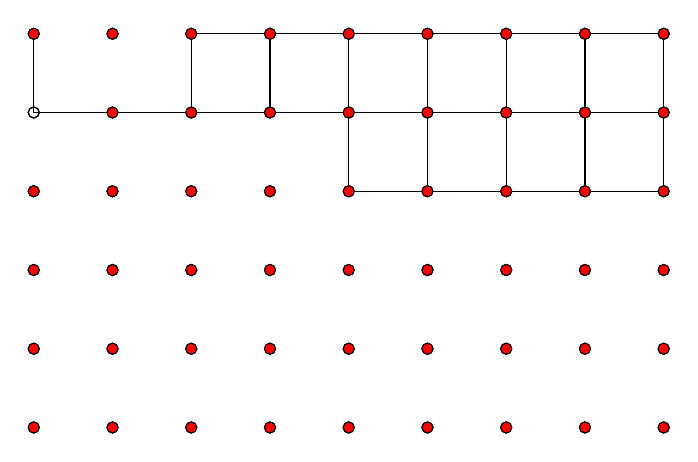
\begin{tikzpicture}[scale=1]%
\path[draw,radius=2pt] (0.0,-8.0) circle;%
\path[draw] (0.0,-7.0) -- (0.0,-8.0);%
\path[draw,radius=2pt] (0.0,-7.0) circle;%
\path[draw] (2.0,-7.0) -- (2.0,-8.0);%
\path[draw] (2.0,-7.0) -- (3.0,-7.0);%
\path[draw,radius=2pt] (2.0,-7.0) circle;%
\path[draw] (3.0,-7.0) -- (3.0,-8.0);%
\path[draw] (3.0,-7.0) -- (2.0,-7.0);%
\path[draw] (3.0,-7.0) -- (4.0,-7.0);%
\path[draw,radius=2pt] (3.0,-7.0) circle;%
\path[draw] (4.0,-7.0) -- (4.0,-8.0);%
\path[draw] (4.0,-7.0) -- (3.0,-7.0);%
\path[draw] (4.0,-7.0) -- (5.0,-7.0);%
\path[draw,radius=2pt] (4.0,-7.0) circle;%
\path[draw] (5.0,-7.0) -- (5.0,-8.0);%
\path[draw] (5.0,-7.0) -- (4.0,-7.0);%
\path[draw] (5.0,-7.0) -- (6.0,-7.0);%
\path[draw,radius=2pt] (5.0,-7.0) circle;%
\path[draw] (6.0,-7.0) -- (6.0,-8.0);%
\path[draw] (6.0,-7.0) -- (5.0,-7.0);%
\path[draw] (6.0,-7.0) -- (7.0,-7.0);%
\path[draw,radius=2pt] (6.0,-7.0) circle;%
\path[draw] (7.0,-7.0) -- (7.0,-8.0);%
\path[draw] (7.0,-7.0) -- (6.0,-7.0);%
\path[draw] (7.0,-7.0) -- (8.0,-7.0);%
\path[draw,radius=2pt] (7.0,-7.0) circle;%
\path[draw] (8.0,-7.0) -- (8.0,-8.0);%
\path[draw] (8.0,-7.0) -- (7.0,-7.0);%
\path[draw,radius=2pt] (8.0,-7.0) circle;%
\path[draw] (0.0,-8.0) -- (0.0,-7.0);%
\path[draw] (0.0,-8.0) -- (1.0,-8.0);%
\path[draw,radius=2pt] (0.0,-8.0) circle;%
\path[draw] (1.0,-8.0) -- (0.0,-8.0);%
\path[draw] (1.0,-8.0) -- (2.0,-8.0);%
\path[draw,radius=2pt] (1.0,-8.0) circle;%
\path[draw] (2.0,-8.0) -- (2.0,-7.0);%
\path[draw] (2.0,-8.0) -- (1.0,-8.0);%
\path[draw] (2.0,-8.0) -- (3.0,-8.0);%
\path[draw,radius=2pt] (2.0,-8.0) circle;%
\path[draw] (3.0,-8.0) -- (3.0,-7.0);%
\path[draw] (3.0,-8.0) -- (2.0,-8.0);%
\path[draw] (3.0,-8.0) -- (4.0,-8.0);%
\path[draw,radius=2pt] (3.0,-8.0) circle;%
\path[draw] (4.0,-8.0) -- (4.0,-7.0);%
\path[draw] (4.0,-8.0) -- (4.0,-9.0);%
\path[draw] (4.0,-8.0) -- (3.0,-8.0);%
\path[draw] (4.0,-8.0) -- (5.0,-8.0);%
\path[draw,radius=2pt] (4.0,-8.0) circle;%
\path[draw] (5.0,-8.0) -- (5.0,-7.0);%
\path[draw] (5.0,-8.0) -- (5.0,-9.0);%
\path[draw] (5.0,-8.0) -- (4.0,-8.0);%
\path[draw] (5.0,-8.0) -- (6.0,-8.0);%
\path[draw,radius=2pt] (5.0,-8.0) circle;%
\path[draw] (6.0,-8.0) -- (6.0,-7.0);%
\path[draw] (6.0,-8.0) -- (6.0,-9.0);%
\path[draw] (6.0,-8.0) -- (5.0,-8.0);%
\path[draw] (6.0,-8.0) -- (7.0,-8.0);%
\path[draw,radius=2pt] (6.0,-8.0) circle;%
\path[draw] (7.0,-8.0) -- (7.0,-7.0);%
\path[draw] (7.0,-8.0) -- (7.0,-9.0);%
\path[draw] (7.0,-8.0) -- (6.0,-8.0);%
\path[draw] (7.0,-8.0) -- (8.0,-8.0);%
\path[draw,radius=2pt] (7.0,-8.0) circle;%
\path[draw] (8.0,-8.0) -- (8.0,-7.0);%
\path[draw] (8.0,-8.0) -- (8.0,-9.0);%
\path[draw] (8.0,-8.0) -- (7.0,-8.0);%
\path[draw,radius=2pt] (8.0,-8.0) circle;%
\path[draw] (4.0,-9.0) -- (4.0,-8.0);%
\path[draw] (4.0,-9.0) -- (5.0,-9.0);%
\path[draw,radius=2pt] (4.0,-9.0) circle;%
\path[draw] (5.0,-9.0) -- (5.0,-8.0);%
\path[draw] (5.0,-9.0) -- (4.0,-9.0);%
\path[draw] (5.0,-9.0) -- (6.0,-9.0);%
\path[draw,radius=2pt] (5.0,-9.0) circle;%
\path[draw] (6.0,-9.0) -- (6.0,-8.0);%
\path[draw] (6.0,-9.0) -- (5.0,-9.0);%
\path[draw] (6.0,-9.0) -- (7.0,-9.0);%
\path[draw,radius=2pt] (6.0,-9.0) circle;%
\path[draw] (7.0,-9.0) -- (7.0,-8.0);%
\path[draw] (7.0,-9.0) -- (6.0,-9.0);%
\path[draw] (7.0,-9.0) -- (8.0,-9.0);%
\path[draw,radius=2pt] (7.0,-9.0) circle;%
\path[draw] (8.0,-9.0) -- (8.0,-8.0);%
\path[draw] (8.0,-9.0) -- (7.0,-9.0);%
\path[draw,radius=2pt] (8.0,-9.0) circle;%
\path[draw,radius=2pt,fill=red] (0.0,-7.0) circle;%
\path[draw,radius=2pt,fill=red] (1.0,-7.0) circle;%
\path[draw,radius=2pt,fill=red] (2.0,-7.0) circle;%
\path[draw,radius=2pt,fill=red] (3.0,-7.0) circle;%
\path[draw,radius=2pt,fill=red] (4.0,-7.0) circle;%
\path[draw,radius=2pt,fill=red] (5.0,-7.0) circle;%
\path[draw,radius=2pt,fill=red] (6.0,-7.0) circle;%
\path[draw,radius=2pt,fill=red] (7.0,-7.0) circle;%
\path[draw,radius=2pt,fill=red] (8.0,-7.0) circle;%
\path[draw,radius=2pt,fill=red] (1.0,-8.0) circle;%
\path[draw,radius=2pt,fill=red] (2.0,-8.0) circle;%
\path[draw,radius=2pt,fill=red] (3.0,-8.0) circle;%
\path[draw,radius=2pt,fill=red] (4.0,-8.0) circle;%
\path[draw,radius=2pt,fill=red] (5.0,-8.0) circle;%
\path[draw,radius=2pt,fill=red] (6.0,-8.0) circle;%
\path[draw,radius=2pt,fill=red] (7.0,-8.0) circle;%
\path[draw,radius=2pt,fill=red] (8.0,-8.0) circle;%
\path[draw,radius=2pt,fill=red] (0.0,-9.0) circle;%
\path[draw,radius=2pt,fill=red] (1.0,-9.0) circle;%
\path[draw,radius=2pt,fill=red] (2.0,-9.0) circle;%
\path[draw,radius=2pt,fill=red] (3.0,-9.0) circle;%
\path[draw,radius=2pt,fill=red] (4.0,-9.0) circle;%
\path[draw,radius=2pt,fill=red] (5.0,-9.0) circle;%
\path[draw,radius=2pt,fill=red] (6.0,-9.0) circle;%
\path[draw,radius=2pt,fill=red] (7.0,-9.0) circle;%
\path[draw,radius=2pt,fill=red] (8.0,-9.0) circle;%
\path[draw,radius=2pt,fill=red] (0.0,-10.0) circle;%
\path[draw,radius=2pt,fill=red] (1.0,-10.0) circle;%
\path[draw,radius=2pt,fill=red] (2.0,-10.0) circle;%
\path[draw,radius=2pt,fill=red] (3.0,-10.0) circle;%
\path[draw,radius=2pt,fill=red] (4.0,-10.0) circle;%
\path[draw,radius=2pt,fill=red] (5.0,-10.0) circle;%
\path[draw,radius=2pt,fill=red] (6.0,-10.0) circle;%
\path[draw,radius=2pt,fill=red] (7.0,-10.0) circle;%
\path[draw,radius=2pt,fill=red] (8.0,-10.0) circle;%
\path[draw,radius=2pt,fill=red] (0.0,-11.0) circle;%
\path[draw,radius=2pt,fill=red] (1.0,-11.0) circle;%
\path[draw,radius=2pt,fill=red] (2.0,-11.0) circle;%
\path[draw,radius=2pt,fill=red] (3.0,-11.0) circle;%
\path[draw,radius=2pt,fill=red] (4.0,-11.0) circle;%
\path[draw,radius=2pt,fill=red] (5.0,-11.0) circle;%
\path[draw,radius=2pt,fill=red] (6.0,-11.0) circle;%
\path[draw,radius=2pt,fill=red] (7.0,-11.0) circle;%
\path[draw,radius=2pt,fill=red] (8.0,-11.0) circle;%
\path[draw,radius=2pt,fill=red] (0.0,-12.0) circle;%
\path[draw,radius=2pt,fill=red] (1.0,-12.0) circle;%
\path[draw,radius=2pt,fill=red] (2.0,-12.0) circle;%
\path[draw,radius=2pt,fill=red] (3.0,-12.0) circle;%
\path[draw,radius=2pt,fill=red] (4.0,-12.0) circle;%
\path[draw,radius=2pt,fill=red] (5.0,-12.0) circle;%
\path[draw,radius=2pt,fill=red] (6.0,-12.0) circle;%
\path[draw,radius=2pt,fill=red] (7.0,-12.0) circle;%
\path[draw,radius=2pt,fill=red] (8.0,-12.0) circle;%
\path[draw,radius=2pt,fill=red] (1.0,-7.0) circle;%
\path[draw,radius=2pt,fill=red] (0.0,-9.0) circle;%
\path[draw,radius=2pt,fill=red] (1.0,-9.0) circle;%
\path[draw,radius=2pt,fill=red] (2.0,-9.0) circle;%
\path[draw,radius=2pt,fill=red] (3.0,-9.0) circle;%
\path[draw,radius=2pt,fill=red] (0.0,-10.0) circle;%
\path[draw,radius=2pt,fill=red] (1.0,-10.0) circle;%
\path[draw,radius=2pt,fill=red] (2.0,-10.0) circle;%
\path[draw,radius=2pt,fill=red] (3.0,-10.0) circle;%
\path[draw,radius=2pt,fill=red] (4.0,-10.0) circle;%
\path[draw,radius=2pt,fill=red] (5.0,-10.0) circle;%
\path[draw,radius=2pt,fill=red] (6.0,-10.0) circle;%
\path[draw,radius=2pt,fill=red] (7.0,-10.0) circle;%
\path[draw,radius=2pt,fill=red] (8.0,-10.0) circle;%
\path[draw,radius=2pt,fill=red] (0.0,-11.0) circle;%
\path[draw,radius=2pt,fill=red] (1.0,-11.0) circle;%
\path[draw,radius=2pt,fill=red] (2.0,-11.0) circle;%
\path[draw,radius=2pt,fill=red] (3.0,-11.0) circle;%
\path[draw,radius=2pt,fill=red] (4.0,-11.0) circle;%
\path[draw,radius=2pt,fill=red] (5.0,-11.0) circle;%
\path[draw,radius=2pt,fill=red] (6.0,-11.0) circle;%
\path[draw,radius=2pt,fill=red] (7.0,-11.0) circle;%
\path[draw,radius=2pt,fill=red] (8.0,-11.0) circle;%
\path[draw,radius=2pt,fill=red] (0.0,-12.0) circle;%
\path[draw,radius=2pt,fill=red] (1.0,-12.0) circle;%
\path[draw,radius=2pt,fill=red] (2.0,-12.0) circle;%
\path[draw,radius=2pt,fill=red] (3.0,-12.0) circle;%
\path[draw,radius=2pt,fill=red] (4.0,-12.0) circle;%
\path[draw,radius=2pt,fill=red] (5.0,-12.0) circle;%
\path[draw,radius=2pt,fill=red] (6.0,-12.0) circle;%
\path[draw,radius=2pt,fill=red] (7.0,-12.0) circle;%
\path[draw,radius=2pt,fill=red] (8.0,-12.0) circle;%
\end{tikzpicture}%
\hspace*{1in}%
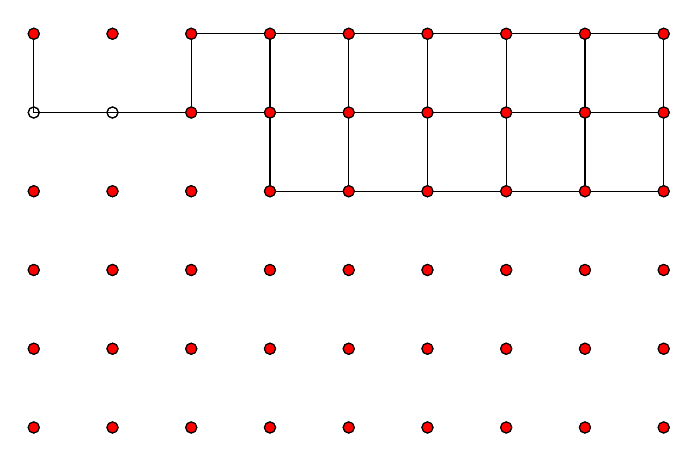
\begin{tikzpicture}[scale=1]%
\path[draw] (0.0,-8.0) -- (1.0,-8.0);%
\path[draw,radius=2pt] (0.0,-8.0) circle;%
\path[draw] (1.0,-8.0) -- (0.0,-8.0);%
\path[draw,radius=2pt] (1.0,-8.0) circle;%
\path[draw] (0.0,-7.0) -- (0.0,-8.0);%
\path[draw,radius=2pt] (0.0,-7.0) circle;%
\path[draw] (2.0,-7.0) -- (2.0,-8.0);%
\path[draw] (2.0,-7.0) -- (3.0,-7.0);%
\path[draw,radius=2pt] (2.0,-7.0) circle;%
\path[draw] (3.0,-7.0) -- (3.0,-8.0);%
\path[draw] (3.0,-7.0) -- (2.0,-7.0);%
\path[draw] (3.0,-7.0) -- (4.0,-7.0);%
\path[draw,radius=2pt] (3.0,-7.0) circle;%
\path[draw] (4.0,-7.0) -- (4.0,-8.0);%
\path[draw] (4.0,-7.0) -- (3.0,-7.0);%
\path[draw] (4.0,-7.0) -- (5.0,-7.0);%
\path[draw,radius=2pt] (4.0,-7.0) circle;%
\path[draw] (5.0,-7.0) -- (5.0,-8.0);%
\path[draw] (5.0,-7.0) -- (4.0,-7.0);%
\path[draw] (5.0,-7.0) -- (6.0,-7.0);%
\path[draw,radius=2pt] (5.0,-7.0) circle;%
\path[draw] (6.0,-7.0) -- (6.0,-8.0);%
\path[draw] (6.0,-7.0) -- (5.0,-7.0);%
\path[draw] (6.0,-7.0) -- (7.0,-7.0);%
\path[draw,radius=2pt] (6.0,-7.0) circle;%
\path[draw] (7.0,-7.0) -- (7.0,-8.0);%
\path[draw] (7.0,-7.0) -- (6.0,-7.0);%
\path[draw] (7.0,-7.0) -- (8.0,-7.0);%
\path[draw,radius=2pt] (7.0,-7.0) circle;%
\path[draw] (8.0,-7.0) -- (8.0,-8.0);%
\path[draw] (8.0,-7.0) -- (7.0,-7.0);%
\path[draw,radius=2pt] (8.0,-7.0) circle;%
\path[draw] (0.0,-8.0) -- (0.0,-7.0);%
\path[draw] (0.0,-8.0) -- (1.0,-8.0);%
\path[draw,radius=2pt] (0.0,-8.0) circle;%
\path[draw] (1.0,-8.0) -- (0.0,-8.0);%
\path[draw] (1.0,-8.0) -- (2.0,-8.0);%
\path[draw,radius=2pt] (1.0,-8.0) circle;%
\path[draw] (2.0,-8.0) -- (2.0,-7.0);%
\path[draw] (2.0,-8.0) -- (1.0,-8.0);%
\path[draw] (2.0,-8.0) -- (3.0,-8.0);%
\path[draw,radius=2pt] (2.0,-8.0) circle;%
\path[draw] (3.0,-8.0) -- (3.0,-7.0);%
\path[draw] (3.0,-8.0) -- (3.0,-9.0);%
\path[draw] (3.0,-8.0) -- (2.0,-8.0);%
\path[draw] (3.0,-8.0) -- (4.0,-8.0);%
\path[draw,radius=2pt] (3.0,-8.0) circle;%
\path[draw] (4.0,-8.0) -- (4.0,-7.0);%
\path[draw] (4.0,-8.0) -- (4.0,-9.0);%
\path[draw] (4.0,-8.0) -- (3.0,-8.0);%
\path[draw] (4.0,-8.0) -- (5.0,-8.0);%
\path[draw,radius=2pt] (4.0,-8.0) circle;%
\path[draw] (5.0,-8.0) -- (5.0,-7.0);%
\path[draw] (5.0,-8.0) -- (5.0,-9.0);%
\path[draw] (5.0,-8.0) -- (4.0,-8.0);%
\path[draw] (5.0,-8.0) -- (6.0,-8.0);%
\path[draw,radius=2pt] (5.0,-8.0) circle;%
\path[draw] (6.0,-8.0) -- (6.0,-7.0);%
\path[draw] (6.0,-8.0) -- (6.0,-9.0);%
\path[draw] (6.0,-8.0) -- (5.0,-8.0);%
\path[draw] (6.0,-8.0) -- (7.0,-8.0);%
\path[draw,radius=2pt] (6.0,-8.0) circle;%
\path[draw] (7.0,-8.0) -- (7.0,-7.0);%
\path[draw] (7.0,-8.0) -- (7.0,-9.0);%
\path[draw] (7.0,-8.0) -- (6.0,-8.0);%
\path[draw] (7.0,-8.0) -- (8.0,-8.0);%
\path[draw,radius=2pt] (7.0,-8.0) circle;%
\path[draw] (8.0,-8.0) -- (8.0,-7.0);%
\path[draw] (8.0,-8.0) -- (8.0,-9.0);%
\path[draw] (8.0,-8.0) -- (7.0,-8.0);%
\path[draw,radius=2pt] (8.0,-8.0) circle;%
\path[draw] (3.0,-9.0) -- (3.0,-8.0);%
\path[draw] (3.0,-9.0) -- (4.0,-9.0);%
\path[draw,radius=2pt] (3.0,-9.0) circle;%
\path[draw] (4.0,-9.0) -- (4.0,-8.0);%
\path[draw] (4.0,-9.0) -- (3.0,-9.0);%
\path[draw] (4.0,-9.0) -- (5.0,-9.0);%
\path[draw,radius=2pt] (4.0,-9.0) circle;%
\path[draw] (5.0,-9.0) -- (5.0,-8.0);%
\path[draw] (5.0,-9.0) -- (4.0,-9.0);%
\path[draw] (5.0,-9.0) -- (6.0,-9.0);%
\path[draw,radius=2pt] (5.0,-9.0) circle;%
\path[draw] (6.0,-9.0) -- (6.0,-8.0);%
\path[draw] (6.0,-9.0) -- (5.0,-9.0);%
\path[draw] (6.0,-9.0) -- (7.0,-9.0);%
\path[draw,radius=2pt] (6.0,-9.0) circle;%
\path[draw] (7.0,-9.0) -- (7.0,-8.0);%
\path[draw] (7.0,-9.0) -- (6.0,-9.0);%
\path[draw] (7.0,-9.0) -- (8.0,-9.0);%
\path[draw,radius=2pt] (7.0,-9.0) circle;%
\path[draw] (8.0,-9.0) -- (8.0,-8.0);%
\path[draw] (8.0,-9.0) -- (7.0,-9.0);%
\path[draw,radius=2pt] (8.0,-9.0) circle;%
\path[draw,radius=2pt,fill=red] (0.0,-7.0) circle;%
\path[draw,radius=2pt,fill=red] (1.0,-7.0) circle;%
\path[draw,radius=2pt,fill=red] (2.0,-7.0) circle;%
\path[draw,radius=2pt,fill=red] (3.0,-7.0) circle;%
\path[draw,radius=2pt,fill=red] (4.0,-7.0) circle;%
\path[draw,radius=2pt,fill=red] (5.0,-7.0) circle;%
\path[draw,radius=2pt,fill=red] (6.0,-7.0) circle;%
\path[draw,radius=2pt,fill=red] (7.0,-7.0) circle;%
\path[draw,radius=2pt,fill=red] (8.0,-7.0) circle;%
\path[draw,radius=2pt,fill=red] (2.0,-8.0) circle;%
\path[draw,radius=2pt,fill=red] (3.0,-8.0) circle;%
\path[draw,radius=2pt,fill=red] (4.0,-8.0) circle;%
\path[draw,radius=2pt,fill=red] (5.0,-8.0) circle;%
\path[draw,radius=2pt,fill=red] (6.0,-8.0) circle;%
\path[draw,radius=2pt,fill=red] (7.0,-8.0) circle;%
\path[draw,radius=2pt,fill=red] (8.0,-8.0) circle;%
\path[draw,radius=2pt,fill=red] (0.0,-9.0) circle;%
\path[draw,radius=2pt,fill=red] (1.0,-9.0) circle;%
\path[draw,radius=2pt,fill=red] (2.0,-9.0) circle;%
\path[draw,radius=2pt,fill=red] (3.0,-9.0) circle;%
\path[draw,radius=2pt,fill=red] (4.0,-9.0) circle;%
\path[draw,radius=2pt,fill=red] (5.0,-9.0) circle;%
\path[draw,radius=2pt,fill=red] (6.0,-9.0) circle;%
\path[draw,radius=2pt,fill=red] (7.0,-9.0) circle;%
\path[draw,radius=2pt,fill=red] (8.0,-9.0) circle;%
\path[draw,radius=2pt,fill=red] (0.0,-10.0) circle;%
\path[draw,radius=2pt,fill=red] (1.0,-10.0) circle;%
\path[draw,radius=2pt,fill=red] (2.0,-10.0) circle;%
\path[draw,radius=2pt,fill=red] (3.0,-10.0) circle;%
\path[draw,radius=2pt,fill=red] (4.0,-10.0) circle;%
\path[draw,radius=2pt,fill=red] (5.0,-10.0) circle;%
\path[draw,radius=2pt,fill=red] (6.0,-10.0) circle;%
\path[draw,radius=2pt,fill=red] (7.0,-10.0) circle;%
\path[draw,radius=2pt,fill=red] (8.0,-10.0) circle;%
\path[draw,radius=2pt,fill=red] (0.0,-11.0) circle;%
\path[draw,radius=2pt,fill=red] (1.0,-11.0) circle;%
\path[draw,radius=2pt,fill=red] (2.0,-11.0) circle;%
\path[draw,radius=2pt,fill=red] (3.0,-11.0) circle;%
\path[draw,radius=2pt,fill=red] (4.0,-11.0) circle;%
\path[draw,radius=2pt,fill=red] (5.0,-11.0) circle;%
\path[draw,radius=2pt,fill=red] (6.0,-11.0) circle;%
\path[draw,radius=2pt,fill=red] (7.0,-11.0) circle;%
\path[draw,radius=2pt,fill=red] (8.0,-11.0) circle;%
\path[draw,radius=2pt,fill=red] (0.0,-12.0) circle;%
\path[draw,radius=2pt,fill=red] (1.0,-12.0) circle;%
\path[draw,radius=2pt,fill=red] (2.0,-12.0) circle;%
\path[draw,radius=2pt,fill=red] (3.0,-12.0) circle;%
\path[draw,radius=2pt,fill=red] (4.0,-12.0) circle;%
\path[draw,radius=2pt,fill=red] (5.0,-12.0) circle;%
\path[draw,radius=2pt,fill=red] (6.0,-12.0) circle;%
\path[draw,radius=2pt,fill=red] (7.0,-12.0) circle;%
\path[draw,radius=2pt,fill=red] (8.0,-12.0) circle;%
\path[draw,radius=2pt,fill=red] (1.0,-7.0) circle;%
\path[draw,radius=2pt,fill=red] (0.0,-9.0) circle;%
\path[draw,radius=2pt,fill=red] (1.0,-9.0) circle;%
\path[draw,radius=2pt,fill=red] (2.0,-9.0) circle;%
\path[draw,radius=2pt,fill=red] (0.0,-10.0) circle;%
\path[draw,radius=2pt,fill=red] (1.0,-10.0) circle;%
\path[draw,radius=2pt,fill=red] (2.0,-10.0) circle;%
\path[draw,radius=2pt,fill=red] (3.0,-10.0) circle;%
\path[draw,radius=2pt,fill=red] (4.0,-10.0) circle;%
\path[draw,radius=2pt,fill=red] (5.0,-10.0) circle;%
\path[draw,radius=2pt,fill=red] (6.0,-10.0) circle;%
\path[draw,radius=2pt,fill=red] (7.0,-10.0) circle;%
\path[draw,radius=2pt,fill=red] (8.0,-10.0) circle;%
\path[draw,radius=2pt,fill=red] (0.0,-11.0) circle;%
\path[draw,radius=2pt,fill=red] (1.0,-11.0) circle;%
\path[draw,radius=2pt,fill=red] (2.0,-11.0) circle;%
\path[draw,radius=2pt,fill=red] (3.0,-11.0) circle;%
\path[draw,radius=2pt,fill=red] (4.0,-11.0) circle;%
\path[draw,radius=2pt,fill=red] (5.0,-11.0) circle;%
\path[draw,radius=2pt,fill=red] (6.0,-11.0) circle;%
\path[draw,radius=2pt,fill=red] (7.0,-11.0) circle;%
\path[draw,radius=2pt,fill=red] (8.0,-11.0) circle;%
\path[draw,radius=2pt,fill=red] (0.0,-12.0) circle;%
\path[draw,radius=2pt,fill=red] (1.0,-12.0) circle;%
\path[draw,radius=2pt,fill=red] (2.0,-12.0) circle;%
\path[draw,radius=2pt,fill=red] (3.0,-12.0) circle;%
\path[draw,radius=2pt,fill=red] (4.0,-12.0) circle;%
\path[draw,radius=2pt,fill=red] (5.0,-12.0) circle;%
\path[draw,radius=2pt,fill=red] (6.0,-12.0) circle;%
\path[draw,radius=2pt,fill=red] (7.0,-12.0) circle;%
\path[draw,radius=2pt,fill=red] (8.0,-12.0) circle;%
\end{tikzpicture}%
\hspace*{1in}%
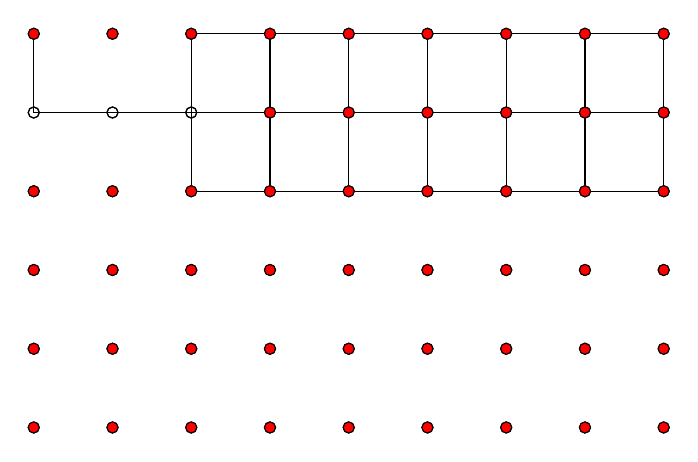
\begin{tikzpicture}[scale=1]%
\path[draw] (0.0,-8.0) -- (1.0,-8.0);%
\path[draw,radius=2pt] (0.0,-8.0) circle;%
\path[draw] (1.0,-8.0) -- (0.0,-8.0);%
\path[draw] (1.0,-8.0) -- (2.0,-8.0);%
\path[draw,radius=2pt] (1.0,-8.0) circle;%
\path[draw] (2.0,-8.0) -- (1.0,-8.0);%
\path[draw,radius=2pt] (2.0,-8.0) circle;%
\path[draw] (0.0,-7.0) -- (0.0,-8.0);%
\path[draw,radius=2pt] (0.0,-7.0) circle;%
\path[draw] (2.0,-7.0) -- (2.0,-8.0);%
\path[draw] (2.0,-7.0) -- (3.0,-7.0);%
\path[draw,radius=2pt] (2.0,-7.0) circle;%
\path[draw] (3.0,-7.0) -- (3.0,-8.0);%
\path[draw] (3.0,-7.0) -- (2.0,-7.0);%
\path[draw] (3.0,-7.0) -- (4.0,-7.0);%
\path[draw,radius=2pt] (3.0,-7.0) circle;%
\path[draw] (4.0,-7.0) -- (4.0,-8.0);%
\path[draw] (4.0,-7.0) -- (3.0,-7.0);%
\path[draw] (4.0,-7.0) -- (5.0,-7.0);%
\path[draw,radius=2pt] (4.0,-7.0) circle;%
\path[draw] (5.0,-7.0) -- (5.0,-8.0);%
\path[draw] (5.0,-7.0) -- (4.0,-7.0);%
\path[draw] (5.0,-7.0) -- (6.0,-7.0);%
\path[draw,radius=2pt] (5.0,-7.0) circle;%
\path[draw] (6.0,-7.0) -- (6.0,-8.0);%
\path[draw] (6.0,-7.0) -- (5.0,-7.0);%
\path[draw] (6.0,-7.0) -- (7.0,-7.0);%
\path[draw,radius=2pt] (6.0,-7.0) circle;%
\path[draw] (7.0,-7.0) -- (7.0,-8.0);%
\path[draw] (7.0,-7.0) -- (6.0,-7.0);%
\path[draw] (7.0,-7.0) -- (8.0,-7.0);%
\path[draw,radius=2pt] (7.0,-7.0) circle;%
\path[draw] (8.0,-7.0) -- (8.0,-8.0);%
\path[draw] (8.0,-7.0) -- (7.0,-7.0);%
\path[draw,radius=2pt] (8.0,-7.0) circle;%
\path[draw] (0.0,-8.0) -- (0.0,-7.0);%
\path[draw] (0.0,-8.0) -- (1.0,-8.0);%
\path[draw,radius=2pt] (0.0,-8.0) circle;%
\path[draw] (1.0,-8.0) -- (0.0,-8.0);%
\path[draw] (1.0,-8.0) -- (2.0,-8.0);%
\path[draw,radius=2pt] (1.0,-8.0) circle;%
\path[draw] (2.0,-8.0) -- (2.0,-7.0);%
\path[draw] (2.0,-8.0) -- (2.0,-9.0);%
\path[draw] (2.0,-8.0) -- (1.0,-8.0);%
\path[draw] (2.0,-8.0) -- (3.0,-8.0);%
\path[draw,radius=2pt] (2.0,-8.0) circle;%
\path[draw] (3.0,-8.0) -- (3.0,-7.0);%
\path[draw] (3.0,-8.0) -- (3.0,-9.0);%
\path[draw] (3.0,-8.0) -- (2.0,-8.0);%
\path[draw] (3.0,-8.0) -- (4.0,-8.0);%
\path[draw,radius=2pt] (3.0,-8.0) circle;%
\path[draw] (4.0,-8.0) -- (4.0,-7.0);%
\path[draw] (4.0,-8.0) -- (4.0,-9.0);%
\path[draw] (4.0,-8.0) -- (3.0,-8.0);%
\path[draw] (4.0,-8.0) -- (5.0,-8.0);%
\path[draw,radius=2pt] (4.0,-8.0) circle;%
\path[draw] (5.0,-8.0) -- (5.0,-7.0);%
\path[draw] (5.0,-8.0) -- (5.0,-9.0);%
\path[draw] (5.0,-8.0) -- (4.0,-8.0);%
\path[draw] (5.0,-8.0) -- (6.0,-8.0);%
\path[draw,radius=2pt] (5.0,-8.0) circle;%
\path[draw] (6.0,-8.0) -- (6.0,-7.0);%
\path[draw] (6.0,-8.0) -- (6.0,-9.0);%
\path[draw] (6.0,-8.0) -- (5.0,-8.0);%
\path[draw] (6.0,-8.0) -- (7.0,-8.0);%
\path[draw,radius=2pt] (6.0,-8.0) circle;%
\path[draw] (7.0,-8.0) -- (7.0,-7.0);%
\path[draw] (7.0,-8.0) -- (7.0,-9.0);%
\path[draw] (7.0,-8.0) -- (6.0,-8.0);%
\path[draw] (7.0,-8.0) -- (8.0,-8.0);%
\path[draw,radius=2pt] (7.0,-8.0) circle;%
\path[draw] (8.0,-8.0) -- (8.0,-7.0);%
\path[draw] (8.0,-8.0) -- (8.0,-9.0);%
\path[draw] (8.0,-8.0) -- (7.0,-8.0);%
\path[draw,radius=2pt] (8.0,-8.0) circle;%
\path[draw] (2.0,-9.0) -- (2.0,-8.0);%
\path[draw] (2.0,-9.0) -- (3.0,-9.0);%
\path[draw,radius=2pt] (2.0,-9.0) circle;%
\path[draw] (3.0,-9.0) -- (3.0,-8.0);%
\path[draw] (3.0,-9.0) -- (2.0,-9.0);%
\path[draw] (3.0,-9.0) -- (4.0,-9.0);%
\path[draw,radius=2pt] (3.0,-9.0) circle;%
\path[draw] (4.0,-9.0) -- (4.0,-8.0);%
\path[draw] (4.0,-9.0) -- (3.0,-9.0);%
\path[draw] (4.0,-9.0) -- (5.0,-9.0);%
\path[draw,radius=2pt] (4.0,-9.0) circle;%
\path[draw] (5.0,-9.0) -- (5.0,-8.0);%
\path[draw] (5.0,-9.0) -- (4.0,-9.0);%
\path[draw] (5.0,-9.0) -- (6.0,-9.0);%
\path[draw,radius=2pt] (5.0,-9.0) circle;%
\path[draw] (6.0,-9.0) -- (6.0,-8.0);%
\path[draw] (6.0,-9.0) -- (5.0,-9.0);%
\path[draw] (6.0,-9.0) -- (7.0,-9.0);%
\path[draw,radius=2pt] (6.0,-9.0) circle;%
\path[draw] (7.0,-9.0) -- (7.0,-8.0);%
\path[draw] (7.0,-9.0) -- (6.0,-9.0);%
\path[draw] (7.0,-9.0) -- (8.0,-9.0);%
\path[draw,radius=2pt] (7.0,-9.0) circle;%
\path[draw] (8.0,-9.0) -- (8.0,-8.0);%
\path[draw] (8.0,-9.0) -- (7.0,-9.0);%
\path[draw,radius=2pt] (8.0,-9.0) circle;%
\path[draw,radius=2pt,fill=red] (0.0,-7.0) circle;%
\path[draw,radius=2pt,fill=red] (1.0,-7.0) circle;%
\path[draw,radius=2pt,fill=red] (2.0,-7.0) circle;%
\path[draw,radius=2pt,fill=red] (3.0,-7.0) circle;%
\path[draw,radius=2pt,fill=red] (4.0,-7.0) circle;%
\path[draw,radius=2pt,fill=red] (5.0,-7.0) circle;%
\path[draw,radius=2pt,fill=red] (6.0,-7.0) circle;%
\path[draw,radius=2pt,fill=red] (7.0,-7.0) circle;%
\path[draw,radius=2pt,fill=red] (8.0,-7.0) circle;%
\path[draw,radius=2pt,fill=red] (3.0,-8.0) circle;%
\path[draw,radius=2pt,fill=red] (4.0,-8.0) circle;%
\path[draw,radius=2pt,fill=red] (5.0,-8.0) circle;%
\path[draw,radius=2pt,fill=red] (6.0,-8.0) circle;%
\path[draw,radius=2pt,fill=red] (7.0,-8.0) circle;%
\path[draw,radius=2pt,fill=red] (8.0,-8.0) circle;%
\path[draw,radius=2pt,fill=red] (0.0,-9.0) circle;%
\path[draw,radius=2pt,fill=red] (1.0,-9.0) circle;%
\path[draw,radius=2pt,fill=red] (2.0,-9.0) circle;%
\path[draw,radius=2pt,fill=red] (3.0,-9.0) circle;%
\path[draw,radius=2pt,fill=red] (4.0,-9.0) circle;%
\path[draw,radius=2pt,fill=red] (5.0,-9.0) circle;%
\path[draw,radius=2pt,fill=red] (6.0,-9.0) circle;%
\path[draw,radius=2pt,fill=red] (7.0,-9.0) circle;%
\path[draw,radius=2pt,fill=red] (8.0,-9.0) circle;%
\path[draw,radius=2pt,fill=red] (0.0,-10.0) circle;%
\path[draw,radius=2pt,fill=red] (1.0,-10.0) circle;%
\path[draw,radius=2pt,fill=red] (2.0,-10.0) circle;%
\path[draw,radius=2pt,fill=red] (3.0,-10.0) circle;%
\path[draw,radius=2pt,fill=red] (4.0,-10.0) circle;%
\path[draw,radius=2pt,fill=red] (5.0,-10.0) circle;%
\path[draw,radius=2pt,fill=red] (6.0,-10.0) circle;%
\path[draw,radius=2pt,fill=red] (7.0,-10.0) circle;%
\path[draw,radius=2pt,fill=red] (8.0,-10.0) circle;%
\path[draw,radius=2pt,fill=red] (0.0,-11.0) circle;%
\path[draw,radius=2pt,fill=red] (1.0,-11.0) circle;%
\path[draw,radius=2pt,fill=red] (2.0,-11.0) circle;%
\path[draw,radius=2pt,fill=red] (3.0,-11.0) circle;%
\path[draw,radius=2pt,fill=red] (4.0,-11.0) circle;%
\path[draw,radius=2pt,fill=red] (5.0,-11.0) circle;%
\path[draw,radius=2pt,fill=red] (6.0,-11.0) circle;%
\path[draw,radius=2pt,fill=red] (7.0,-11.0) circle;%
\path[draw,radius=2pt,fill=red] (8.0,-11.0) circle;%
\path[draw,radius=2pt,fill=red] (0.0,-12.0) circle;%
\path[draw,radius=2pt,fill=red] (1.0,-12.0) circle;%
\path[draw,radius=2pt,fill=red] (2.0,-12.0) circle;%
\path[draw,radius=2pt,fill=red] (3.0,-12.0) circle;%
\path[draw,radius=2pt,fill=red] (4.0,-12.0) circle;%
\path[draw,radius=2pt,fill=red] (5.0,-12.0) circle;%
\path[draw,radius=2pt,fill=red] (6.0,-12.0) circle;%
\path[draw,radius=2pt,fill=red] (7.0,-12.0) circle;%
\path[draw,radius=2pt,fill=red] (8.0,-12.0) circle;%
\path[draw,radius=2pt,fill=red] (1.0,-7.0) circle;%
\path[draw,radius=2pt,fill=red] (0.0,-9.0) circle;%
\path[draw,radius=2pt,fill=red] (1.0,-9.0) circle;%
\path[draw,radius=2pt,fill=red] (0.0,-10.0) circle;%
\path[draw,radius=2pt,fill=red] (1.0,-10.0) circle;%
\path[draw,radius=2pt,fill=red] (2.0,-10.0) circle;%
\path[draw,radius=2pt,fill=red] (3.0,-10.0) circle;%
\path[draw,radius=2pt,fill=red] (4.0,-10.0) circle;%
\path[draw,radius=2pt,fill=red] (5.0,-10.0) circle;%
\path[draw,radius=2pt,fill=red] (6.0,-10.0) circle;%
\path[draw,radius=2pt,fill=red] (7.0,-10.0) circle;%
\path[draw,radius=2pt,fill=red] (8.0,-10.0) circle;%
\path[draw,radius=2pt,fill=red] (0.0,-11.0) circle;%
\path[draw,radius=2pt,fill=red] (1.0,-11.0) circle;%
\path[draw,radius=2pt,fill=red] (2.0,-11.0) circle;%
\path[draw,radius=2pt,fill=red] (3.0,-11.0) circle;%
\path[draw,radius=2pt,fill=red] (4.0,-11.0) circle;%
\path[draw,radius=2pt,fill=red] (5.0,-11.0) circle;%
\path[draw,radius=2pt,fill=red] (6.0,-11.0) circle;%
\path[draw,radius=2pt,fill=red] (7.0,-11.0) circle;%
\path[draw,radius=2pt,fill=red] (8.0,-11.0) circle;%
\path[draw,radius=2pt,fill=red] (0.0,-12.0) circle;%
\path[draw,radius=2pt,fill=red] (1.0,-12.0) circle;%
\path[draw,radius=2pt,fill=red] (2.0,-12.0) circle;%
\path[draw,radius=2pt,fill=red] (3.0,-12.0) circle;%
\path[draw,radius=2pt,fill=red] (4.0,-12.0) circle;%
\path[draw,radius=2pt,fill=red] (5.0,-12.0) circle;%
\path[draw,radius=2pt,fill=red] (6.0,-12.0) circle;%
\path[draw,radius=2pt,fill=red] (7.0,-12.0) circle;%
\path[draw,radius=2pt,fill=red] (8.0,-12.0) circle;%
\end{tikzpicture}%
\newline%
\hspace*{1in}%
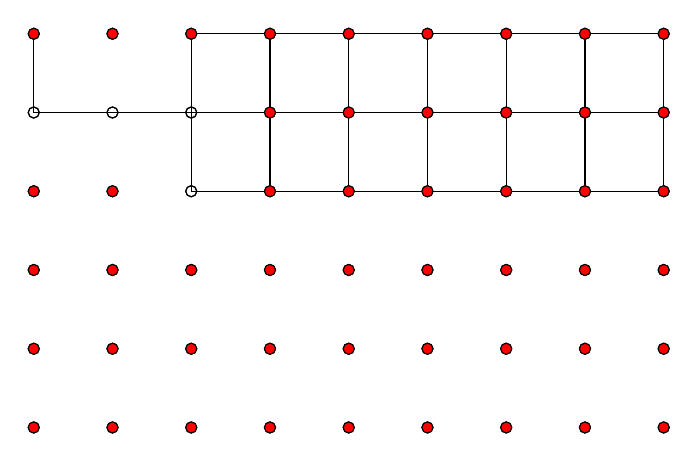
\begin{tikzpicture}[scale=1]%
\path[draw] (0.0,-8.0) -- (1.0,-8.0);%
\path[draw,radius=2pt] (0.0,-8.0) circle;%
\path[draw] (1.0,-8.0) -- (0.0,-8.0);%
\path[draw] (1.0,-8.0) -- (2.0,-8.0);%
\path[draw,radius=2pt] (1.0,-8.0) circle;%
\path[draw] (2.0,-8.0) -- (2.0,-9.0);%
\path[draw] (2.0,-8.0) -- (1.0,-8.0);%
\path[draw,radius=2pt] (2.0,-8.0) circle;%
\path[draw] (2.0,-9.0) -- (2.0,-8.0);%
\path[draw,radius=2pt] (2.0,-9.0) circle;%
\path[draw] (0.0,-7.0) -- (0.0,-8.0);%
\path[draw,radius=2pt] (0.0,-7.0) circle;%
\path[draw] (2.0,-7.0) -- (2.0,-8.0);%
\path[draw] (2.0,-7.0) -- (3.0,-7.0);%
\path[draw,radius=2pt] (2.0,-7.0) circle;%
\path[draw] (3.0,-7.0) -- (3.0,-8.0);%
\path[draw] (3.0,-7.0) -- (2.0,-7.0);%
\path[draw] (3.0,-7.0) -- (4.0,-7.0);%
\path[draw,radius=2pt] (3.0,-7.0) circle;%
\path[draw] (4.0,-7.0) -- (4.0,-8.0);%
\path[draw] (4.0,-7.0) -- (3.0,-7.0);%
\path[draw] (4.0,-7.0) -- (5.0,-7.0);%
\path[draw,radius=2pt] (4.0,-7.0) circle;%
\path[draw] (5.0,-7.0) -- (5.0,-8.0);%
\path[draw] (5.0,-7.0) -- (4.0,-7.0);%
\path[draw] (5.0,-7.0) -- (6.0,-7.0);%
\path[draw,radius=2pt] (5.0,-7.0) circle;%
\path[draw] (6.0,-7.0) -- (6.0,-8.0);%
\path[draw] (6.0,-7.0) -- (5.0,-7.0);%
\path[draw] (6.0,-7.0) -- (7.0,-7.0);%
\path[draw,radius=2pt] (6.0,-7.0) circle;%
\path[draw] (7.0,-7.0) -- (7.0,-8.0);%
\path[draw] (7.0,-7.0) -- (6.0,-7.0);%
\path[draw] (7.0,-7.0) -- (8.0,-7.0);%
\path[draw,radius=2pt] (7.0,-7.0) circle;%
\path[draw] (8.0,-7.0) -- (8.0,-8.0);%
\path[draw] (8.0,-7.0) -- (7.0,-7.0);%
\path[draw,radius=2pt] (8.0,-7.0) circle;%
\path[draw] (0.0,-8.0) -- (0.0,-7.0);%
\path[draw] (0.0,-8.0) -- (1.0,-8.0);%
\path[draw,radius=2pt] (0.0,-8.0) circle;%
\path[draw] (1.0,-8.0) -- (0.0,-8.0);%
\path[draw] (1.0,-8.0) -- (2.0,-8.0);%
\path[draw,radius=2pt] (1.0,-8.0) circle;%
\path[draw] (2.0,-8.0) -- (2.0,-7.0);%
\path[draw] (2.0,-8.0) -- (2.0,-9.0);%
\path[draw] (2.0,-8.0) -- (1.0,-8.0);%
\path[draw] (2.0,-8.0) -- (3.0,-8.0);%
\path[draw,radius=2pt] (2.0,-8.0) circle;%
\path[draw] (3.0,-8.0) -- (3.0,-7.0);%
\path[draw] (3.0,-8.0) -- (3.0,-9.0);%
\path[draw] (3.0,-8.0) -- (2.0,-8.0);%
\path[draw] (3.0,-8.0) -- (4.0,-8.0);%
\path[draw,radius=2pt] (3.0,-8.0) circle;%
\path[draw] (4.0,-8.0) -- (4.0,-7.0);%
\path[draw] (4.0,-8.0) -- (4.0,-9.0);%
\path[draw] (4.0,-8.0) -- (3.0,-8.0);%
\path[draw] (4.0,-8.0) -- (5.0,-8.0);%
\path[draw,radius=2pt] (4.0,-8.0) circle;%
\path[draw] (5.0,-8.0) -- (5.0,-7.0);%
\path[draw] (5.0,-8.0) -- (5.0,-9.0);%
\path[draw] (5.0,-8.0) -- (4.0,-8.0);%
\path[draw] (5.0,-8.0) -- (6.0,-8.0);%
\path[draw,radius=2pt] (5.0,-8.0) circle;%
\path[draw] (6.0,-8.0) -- (6.0,-7.0);%
\path[draw] (6.0,-8.0) -- (6.0,-9.0);%
\path[draw] (6.0,-8.0) -- (5.0,-8.0);%
\path[draw] (6.0,-8.0) -- (7.0,-8.0);%
\path[draw,radius=2pt] (6.0,-8.0) circle;%
\path[draw] (7.0,-8.0) -- (7.0,-7.0);%
\path[draw] (7.0,-8.0) -- (7.0,-9.0);%
\path[draw] (7.0,-8.0) -- (6.0,-8.0);%
\path[draw] (7.0,-8.0) -- (8.0,-8.0);%
\path[draw,radius=2pt] (7.0,-8.0) circle;%
\path[draw] (8.0,-8.0) -- (8.0,-7.0);%
\path[draw] (8.0,-8.0) -- (8.0,-9.0);%
\path[draw] (8.0,-8.0) -- (7.0,-8.0);%
\path[draw,radius=2pt] (8.0,-8.0) circle;%
\path[draw] (2.0,-9.0) -- (2.0,-8.0);%
\path[draw] (2.0,-9.0) -- (3.0,-9.0);%
\path[draw,radius=2pt] (2.0,-9.0) circle;%
\path[draw] (3.0,-9.0) -- (3.0,-8.0);%
\path[draw] (3.0,-9.0) -- (2.0,-9.0);%
\path[draw] (3.0,-9.0) -- (4.0,-9.0);%
\path[draw,radius=2pt] (3.0,-9.0) circle;%
\path[draw] (4.0,-9.0) -- (4.0,-8.0);%
\path[draw] (4.0,-9.0) -- (3.0,-9.0);%
\path[draw] (4.0,-9.0) -- (5.0,-9.0);%
\path[draw,radius=2pt] (4.0,-9.0) circle;%
\path[draw] (5.0,-9.0) -- (5.0,-8.0);%
\path[draw] (5.0,-9.0) -- (4.0,-9.0);%
\path[draw] (5.0,-9.0) -- (6.0,-9.0);%
\path[draw,radius=2pt] (5.0,-9.0) circle;%
\path[draw] (6.0,-9.0) -- (6.0,-8.0);%
\path[draw] (6.0,-9.0) -- (5.0,-9.0);%
\path[draw] (6.0,-9.0) -- (7.0,-9.0);%
\path[draw,radius=2pt] (6.0,-9.0) circle;%
\path[draw] (7.0,-9.0) -- (7.0,-8.0);%
\path[draw] (7.0,-9.0) -- (6.0,-9.0);%
\path[draw] (7.0,-9.0) -- (8.0,-9.0);%
\path[draw,radius=2pt] (7.0,-9.0) circle;%
\path[draw] (8.0,-9.0) -- (8.0,-8.0);%
\path[draw] (8.0,-9.0) -- (7.0,-9.0);%
\path[draw,radius=2pt] (8.0,-9.0) circle;%
\path[draw,radius=2pt,fill=red] (0.0,-7.0) circle;%
\path[draw,radius=2pt,fill=red] (1.0,-7.0) circle;%
\path[draw,radius=2pt,fill=red] (2.0,-7.0) circle;%
\path[draw,radius=2pt,fill=red] (3.0,-7.0) circle;%
\path[draw,radius=2pt,fill=red] (4.0,-7.0) circle;%
\path[draw,radius=2pt,fill=red] (5.0,-7.0) circle;%
\path[draw,radius=2pt,fill=red] (6.0,-7.0) circle;%
\path[draw,radius=2pt,fill=red] (7.0,-7.0) circle;%
\path[draw,radius=2pt,fill=red] (8.0,-7.0) circle;%
\path[draw,radius=2pt,fill=red] (3.0,-8.0) circle;%
\path[draw,radius=2pt,fill=red] (4.0,-8.0) circle;%
\path[draw,radius=2pt,fill=red] (5.0,-8.0) circle;%
\path[draw,radius=2pt,fill=red] (6.0,-8.0) circle;%
\path[draw,radius=2pt,fill=red] (7.0,-8.0) circle;%
\path[draw,radius=2pt,fill=red] (8.0,-8.0) circle;%
\path[draw,radius=2pt,fill=red] (0.0,-9.0) circle;%
\path[draw,radius=2pt,fill=red] (1.0,-9.0) circle;%
\path[draw,radius=2pt,fill=red] (3.0,-9.0) circle;%
\path[draw,radius=2pt,fill=red] (4.0,-9.0) circle;%
\path[draw,radius=2pt,fill=red] (5.0,-9.0) circle;%
\path[draw,radius=2pt,fill=red] (6.0,-9.0) circle;%
\path[draw,radius=2pt,fill=red] (7.0,-9.0) circle;%
\path[draw,radius=2pt,fill=red] (8.0,-9.0) circle;%
\path[draw,radius=2pt,fill=red] (0.0,-10.0) circle;%
\path[draw,radius=2pt,fill=red] (1.0,-10.0) circle;%
\path[draw,radius=2pt,fill=red] (2.0,-10.0) circle;%
\path[draw,radius=2pt,fill=red] (3.0,-10.0) circle;%
\path[draw,radius=2pt,fill=red] (4.0,-10.0) circle;%
\path[draw,radius=2pt,fill=red] (5.0,-10.0) circle;%
\path[draw,radius=2pt,fill=red] (6.0,-10.0) circle;%
\path[draw,radius=2pt,fill=red] (7.0,-10.0) circle;%
\path[draw,radius=2pt,fill=red] (8.0,-10.0) circle;%
\path[draw,radius=2pt,fill=red] (0.0,-11.0) circle;%
\path[draw,radius=2pt,fill=red] (1.0,-11.0) circle;%
\path[draw,radius=2pt,fill=red] (2.0,-11.0) circle;%
\path[draw,radius=2pt,fill=red] (3.0,-11.0) circle;%
\path[draw,radius=2pt,fill=red] (4.0,-11.0) circle;%
\path[draw,radius=2pt,fill=red] (5.0,-11.0) circle;%
\path[draw,radius=2pt,fill=red] (6.0,-11.0) circle;%
\path[draw,radius=2pt,fill=red] (7.0,-11.0) circle;%
\path[draw,radius=2pt,fill=red] (8.0,-11.0) circle;%
\path[draw,radius=2pt,fill=red] (0.0,-12.0) circle;%
\path[draw,radius=2pt,fill=red] (1.0,-12.0) circle;%
\path[draw,radius=2pt,fill=red] (2.0,-12.0) circle;%
\path[draw,radius=2pt,fill=red] (3.0,-12.0) circle;%
\path[draw,radius=2pt,fill=red] (4.0,-12.0) circle;%
\path[draw,radius=2pt,fill=red] (5.0,-12.0) circle;%
\path[draw,radius=2pt,fill=red] (6.0,-12.0) circle;%
\path[draw,radius=2pt,fill=red] (7.0,-12.0) circle;%
\path[draw,radius=2pt,fill=red] (8.0,-12.0) circle;%
\path[draw,radius=2pt,fill=red] (1.0,-7.0) circle;%
\path[draw,radius=2pt,fill=red] (0.0,-9.0) circle;%
\path[draw,radius=2pt,fill=red] (1.0,-9.0) circle;%
\path[draw,radius=2pt,fill=red] (0.0,-10.0) circle;%
\path[draw,radius=2pt,fill=red] (1.0,-10.0) circle;%
\path[draw,radius=2pt,fill=red] (2.0,-10.0) circle;%
\path[draw,radius=2pt,fill=red] (3.0,-10.0) circle;%
\path[draw,radius=2pt,fill=red] (4.0,-10.0) circle;%
\path[draw,radius=2pt,fill=red] (5.0,-10.0) circle;%
\path[draw,radius=2pt,fill=red] (6.0,-10.0) circle;%
\path[draw,radius=2pt,fill=red] (7.0,-10.0) circle;%
\path[draw,radius=2pt,fill=red] (8.0,-10.0) circle;%
\path[draw,radius=2pt,fill=red] (0.0,-11.0) circle;%
\path[draw,radius=2pt,fill=red] (1.0,-11.0) circle;%
\path[draw,radius=2pt,fill=red] (2.0,-11.0) circle;%
\path[draw,radius=2pt,fill=red] (3.0,-11.0) circle;%
\path[draw,radius=2pt,fill=red] (4.0,-11.0) circle;%
\path[draw,radius=2pt,fill=red] (5.0,-11.0) circle;%
\path[draw,radius=2pt,fill=red] (6.0,-11.0) circle;%
\path[draw,radius=2pt,fill=red] (7.0,-11.0) circle;%
\path[draw,radius=2pt,fill=red] (8.0,-11.0) circle;%
\path[draw,radius=2pt,fill=red] (0.0,-12.0) circle;%
\path[draw,radius=2pt,fill=red] (1.0,-12.0) circle;%
\path[draw,radius=2pt,fill=red] (2.0,-12.0) circle;%
\path[draw,radius=2pt,fill=red] (3.0,-12.0) circle;%
\path[draw,radius=2pt,fill=red] (4.0,-12.0) circle;%
\path[draw,radius=2pt,fill=red] (5.0,-12.0) circle;%
\path[draw,radius=2pt,fill=red] (6.0,-12.0) circle;%
\path[draw,radius=2pt,fill=red] (7.0,-12.0) circle;%
\path[draw,radius=2pt,fill=red] (8.0,-12.0) circle;%
\end{tikzpicture}%
\hspace*{1in}%
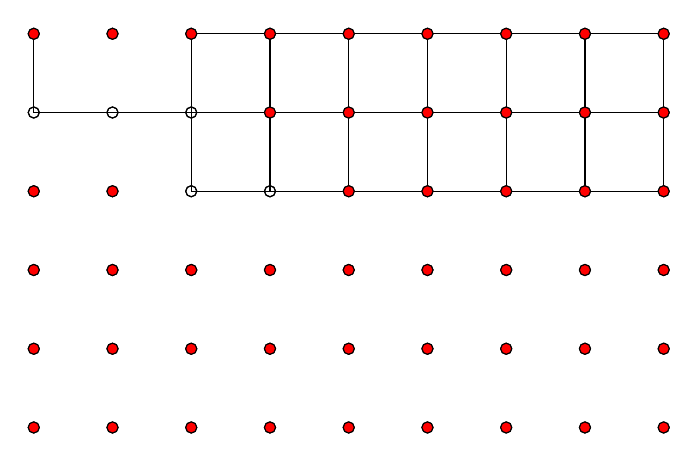
\begin{tikzpicture}[scale=1]%
\path[draw] (0.0,-8.0) -- (1.0,-8.0);%
\path[draw,radius=2pt] (0.0,-8.0) circle;%
\path[draw] (1.0,-8.0) -- (0.0,-8.0);%
\path[draw] (1.0,-8.0) -- (2.0,-8.0);%
\path[draw,radius=2pt] (1.0,-8.0) circle;%
\path[draw] (2.0,-8.0) -- (2.0,-9.0);%
\path[draw] (2.0,-8.0) -- (1.0,-8.0);%
\path[draw,radius=2pt] (2.0,-8.0) circle;%
\path[draw] (2.0,-9.0) -- (2.0,-8.0);%
\path[draw] (2.0,-9.0) -- (3.0,-9.0);%
\path[draw,radius=2pt] (2.0,-9.0) circle;%
\path[draw] (3.0,-9.0) -- (2.0,-9.0);%
\path[draw,radius=2pt] (3.0,-9.0) circle;%
\path[draw,radius=2pt] (8.0,-12.0) circle;%
\path[draw] (0.0,-7.0) -- (0.0,-8.0);%
\path[draw,radius=2pt] (0.0,-7.0) circle;%
\path[draw] (2.0,-7.0) -- (2.0,-8.0);%
\path[draw] (2.0,-7.0) -- (3.0,-7.0);%
\path[draw,radius=2pt] (2.0,-7.0) circle;%
\path[draw] (3.0,-7.0) -- (3.0,-8.0);%
\path[draw] (3.0,-7.0) -- (2.0,-7.0);%
\path[draw] (3.0,-7.0) -- (4.0,-7.0);%
\path[draw,radius=2pt] (3.0,-7.0) circle;%
\path[draw] (4.0,-7.0) -- (4.0,-8.0);%
\path[draw] (4.0,-7.0) -- (3.0,-7.0);%
\path[draw] (4.0,-7.0) -- (5.0,-7.0);%
\path[draw,radius=2pt] (4.0,-7.0) circle;%
\path[draw] (5.0,-7.0) -- (5.0,-8.0);%
\path[draw] (5.0,-7.0) -- (4.0,-7.0);%
\path[draw] (5.0,-7.0) -- (6.0,-7.0);%
\path[draw,radius=2pt] (5.0,-7.0) circle;%
\path[draw] (6.0,-7.0) -- (6.0,-8.0);%
\path[draw] (6.0,-7.0) -- (5.0,-7.0);%
\path[draw] (6.0,-7.0) -- (7.0,-7.0);%
\path[draw,radius=2pt] (6.0,-7.0) circle;%
\path[draw] (7.0,-7.0) -- (7.0,-8.0);%
\path[draw] (7.0,-7.0) -- (6.0,-7.0);%
\path[draw] (7.0,-7.0) -- (8.0,-7.0);%
\path[draw,radius=2pt] (7.0,-7.0) circle;%
\path[draw] (8.0,-7.0) -- (8.0,-8.0);%
\path[draw] (8.0,-7.0) -- (7.0,-7.0);%
\path[draw,radius=2pt] (8.0,-7.0) circle;%
\path[draw] (0.0,-8.0) -- (0.0,-7.0);%
\path[draw] (0.0,-8.0) -- (1.0,-8.0);%
\path[draw,radius=2pt] (0.0,-8.0) circle;%
\path[draw] (1.0,-8.0) -- (0.0,-8.0);%
\path[draw] (1.0,-8.0) -- (2.0,-8.0);%
\path[draw,radius=2pt] (1.0,-8.0) circle;%
\path[draw] (2.0,-8.0) -- (2.0,-7.0);%
\path[draw] (2.0,-8.0) -- (2.0,-9.0);%
\path[draw] (2.0,-8.0) -- (1.0,-8.0);%
\path[draw] (2.0,-8.0) -- (3.0,-8.0);%
\path[draw,radius=2pt] (2.0,-8.0) circle;%
\path[draw] (3.0,-8.0) -- (3.0,-7.0);%
\path[draw] (3.0,-8.0) -- (3.0,-9.0);%
\path[draw] (3.0,-8.0) -- (2.0,-8.0);%
\path[draw] (3.0,-8.0) -- (4.0,-8.0);%
\path[draw,radius=2pt] (3.0,-8.0) circle;%
\path[draw] (4.0,-8.0) -- (4.0,-7.0);%
\path[draw] (4.0,-8.0) -- (4.0,-9.0);%
\path[draw] (4.0,-8.0) -- (3.0,-8.0);%
\path[draw] (4.0,-8.0) -- (5.0,-8.0);%
\path[draw,radius=2pt] (4.0,-8.0) circle;%
\path[draw] (5.0,-8.0) -- (5.0,-7.0);%
\path[draw] (5.0,-8.0) -- (5.0,-9.0);%
\path[draw] (5.0,-8.0) -- (4.0,-8.0);%
\path[draw] (5.0,-8.0) -- (6.0,-8.0);%
\path[draw,radius=2pt] (5.0,-8.0) circle;%
\path[draw] (6.0,-8.0) -- (6.0,-7.0);%
\path[draw] (6.0,-8.0) -- (6.0,-9.0);%
\path[draw] (6.0,-8.0) -- (5.0,-8.0);%
\path[draw] (6.0,-8.0) -- (7.0,-8.0);%
\path[draw,radius=2pt] (6.0,-8.0) circle;%
\path[draw] (7.0,-8.0) -- (7.0,-7.0);%
\path[draw] (7.0,-8.0) -- (7.0,-9.0);%
\path[draw] (7.0,-8.0) -- (6.0,-8.0);%
\path[draw] (7.0,-8.0) -- (8.0,-8.0);%
\path[draw,radius=2pt] (7.0,-8.0) circle;%
\path[draw] (8.0,-8.0) -- (8.0,-7.0);%
\path[draw] (8.0,-8.0) -- (8.0,-9.0);%
\path[draw] (8.0,-8.0) -- (7.0,-8.0);%
\path[draw,radius=2pt] (8.0,-8.0) circle;%
\path[draw] (2.0,-9.0) -- (2.0,-8.0);%
\path[draw] (2.0,-9.0) -- (3.0,-9.0);%
\path[draw,radius=2pt] (2.0,-9.0) circle;%
\path[draw] (3.0,-9.0) -- (3.0,-8.0);%
\path[draw] (3.0,-9.0) -- (2.0,-9.0);%
\path[draw] (3.0,-9.0) -- (4.0,-9.0);%
\path[draw,radius=2pt] (3.0,-9.0) circle;%
\path[draw] (4.0,-9.0) -- (4.0,-8.0);%
\path[draw] (4.0,-9.0) -- (3.0,-9.0);%
\path[draw] (4.0,-9.0) -- (5.0,-9.0);%
\path[draw,radius=2pt] (4.0,-9.0) circle;%
\path[draw] (5.0,-9.0) -- (5.0,-8.0);%
\path[draw] (5.0,-9.0) -- (4.0,-9.0);%
\path[draw] (5.0,-9.0) -- (6.0,-9.0);%
\path[draw,radius=2pt] (5.0,-9.0) circle;%
\path[draw] (6.0,-9.0) -- (6.0,-8.0);%
\path[draw] (6.0,-9.0) -- (5.0,-9.0);%
\path[draw] (6.0,-9.0) -- (7.0,-9.0);%
\path[draw,radius=2pt] (6.0,-9.0) circle;%
\path[draw] (7.0,-9.0) -- (7.0,-8.0);%
\path[draw] (7.0,-9.0) -- (6.0,-9.0);%
\path[draw] (7.0,-9.0) -- (8.0,-9.0);%
\path[draw,radius=2pt] (7.0,-9.0) circle;%
\path[draw] (8.0,-9.0) -- (8.0,-8.0);%
\path[draw] (8.0,-9.0) -- (7.0,-9.0);%
\path[draw,radius=2pt] (8.0,-9.0) circle;%
\path[draw,radius=2pt,fill=red] (0.0,-7.0) circle;%
\path[draw,radius=2pt,fill=red] (1.0,-7.0) circle;%
\path[draw,radius=2pt,fill=red] (2.0,-7.0) circle;%
\path[draw,radius=2pt,fill=red] (3.0,-7.0) circle;%
\path[draw,radius=2pt,fill=red] (4.0,-7.0) circle;%
\path[draw,radius=2pt,fill=red] (5.0,-7.0) circle;%
\path[draw,radius=2pt,fill=red] (6.0,-7.0) circle;%
\path[draw,radius=2pt,fill=red] (7.0,-7.0) circle;%
\path[draw,radius=2pt,fill=red] (8.0,-7.0) circle;%
\path[draw,radius=2pt,fill=red] (3.0,-8.0) circle;%
\path[draw,radius=2pt,fill=red] (4.0,-8.0) circle;%
\path[draw,radius=2pt,fill=red] (5.0,-8.0) circle;%
\path[draw,radius=2pt,fill=red] (6.0,-8.0) circle;%
\path[draw,radius=2pt,fill=red] (7.0,-8.0) circle;%
\path[draw,radius=2pt,fill=red] (8.0,-8.0) circle;%
\path[draw,radius=2pt,fill=red] (0.0,-9.0) circle;%
\path[draw,radius=2pt,fill=red] (1.0,-9.0) circle;%
\path[draw,radius=2pt,fill=red] (4.0,-9.0) circle;%
\path[draw,radius=2pt,fill=red] (5.0,-9.0) circle;%
\path[draw,radius=2pt,fill=red] (6.0,-9.0) circle;%
\path[draw,radius=2pt,fill=red] (7.0,-9.0) circle;%
\path[draw,radius=2pt,fill=red] (8.0,-9.0) circle;%
\path[draw,radius=2pt,fill=red] (0.0,-10.0) circle;%
\path[draw,radius=2pt,fill=red] (1.0,-10.0) circle;%
\path[draw,radius=2pt,fill=red] (2.0,-10.0) circle;%
\path[draw,radius=2pt,fill=red] (3.0,-10.0) circle;%
\path[draw,radius=2pt,fill=red] (4.0,-10.0) circle;%
\path[draw,radius=2pt,fill=red] (5.0,-10.0) circle;%
\path[draw,radius=2pt,fill=red] (6.0,-10.0) circle;%
\path[draw,radius=2pt,fill=red] (7.0,-10.0) circle;%
\path[draw,radius=2pt,fill=red] (8.0,-10.0) circle;%
\path[draw,radius=2pt,fill=red] (0.0,-11.0) circle;%
\path[draw,radius=2pt,fill=red] (1.0,-11.0) circle;%
\path[draw,radius=2pt,fill=red] (2.0,-11.0) circle;%
\path[draw,radius=2pt,fill=red] (3.0,-11.0) circle;%
\path[draw,radius=2pt,fill=red] (4.0,-11.0) circle;%
\path[draw,radius=2pt,fill=red] (5.0,-11.0) circle;%
\path[draw,radius=2pt,fill=red] (6.0,-11.0) circle;%
\path[draw,radius=2pt,fill=red] (7.0,-11.0) circle;%
\path[draw,radius=2pt,fill=red] (8.0,-11.0) circle;%
\path[draw,radius=2pt,fill=red] (0.0,-12.0) circle;%
\path[draw,radius=2pt,fill=red] (1.0,-12.0) circle;%
\path[draw,radius=2pt,fill=red] (2.0,-12.0) circle;%
\path[draw,radius=2pt,fill=red] (3.0,-12.0) circle;%
\path[draw,radius=2pt,fill=red] (4.0,-12.0) circle;%
\path[draw,radius=2pt,fill=red] (5.0,-12.0) circle;%
\path[draw,radius=2pt,fill=red] (6.0,-12.0) circle;%
\path[draw,radius=2pt,fill=red] (7.0,-12.0) circle;%
\path[draw,radius=2pt,fill=red] (1.0,-7.0) circle;%
\path[draw,radius=2pt,fill=red] (0.0,-9.0) circle;%
\path[draw,radius=2pt,fill=red] (1.0,-9.0) circle;%
\path[draw,radius=2pt,fill=red] (0.0,-10.0) circle;%
\path[draw,radius=2pt,fill=red] (1.0,-10.0) circle;%
\path[draw,radius=2pt,fill=red] (2.0,-10.0) circle;%
\path[draw,radius=2pt,fill=red] (3.0,-10.0) circle;%
\path[draw,radius=2pt,fill=red] (4.0,-10.0) circle;%
\path[draw,radius=2pt,fill=red] (5.0,-10.0) circle;%
\path[draw,radius=2pt,fill=red] (6.0,-10.0) circle;%
\path[draw,radius=2pt,fill=red] (7.0,-10.0) circle;%
\path[draw,radius=2pt,fill=red] (8.0,-10.0) circle;%
\path[draw,radius=2pt,fill=red] (0.0,-11.0) circle;%
\path[draw,radius=2pt,fill=red] (1.0,-11.0) circle;%
\path[draw,radius=2pt,fill=red] (2.0,-11.0) circle;%
\path[draw,radius=2pt,fill=red] (3.0,-11.0) circle;%
\path[draw,radius=2pt,fill=red] (4.0,-11.0) circle;%
\path[draw,radius=2pt,fill=red] (5.0,-11.0) circle;%
\path[draw,radius=2pt,fill=red] (6.0,-11.0) circle;%
\path[draw,radius=2pt,fill=red] (7.0,-11.0) circle;%
\path[draw,radius=2pt,fill=red] (8.0,-11.0) circle;%
\path[draw,radius=2pt,fill=red] (0.0,-12.0) circle;%
\path[draw,radius=2pt,fill=red] (1.0,-12.0) circle;%
\path[draw,radius=2pt,fill=red] (2.0,-12.0) circle;%
\path[draw,radius=2pt,fill=red] (3.0,-12.0) circle;%
\path[draw,radius=2pt,fill=red] (4.0,-12.0) circle;%
\path[draw,radius=2pt,fill=red] (5.0,-12.0) circle;%
\path[draw,radius=2pt,fill=red] (6.0,-12.0) circle;%
\path[draw,radius=2pt,fill=red] (7.0,-12.0) circle;%
\path[draw,radius=2pt,fill=red] (8.0,-12.0) circle;%
\end{tikzpicture}%
\hspace*{1in}%
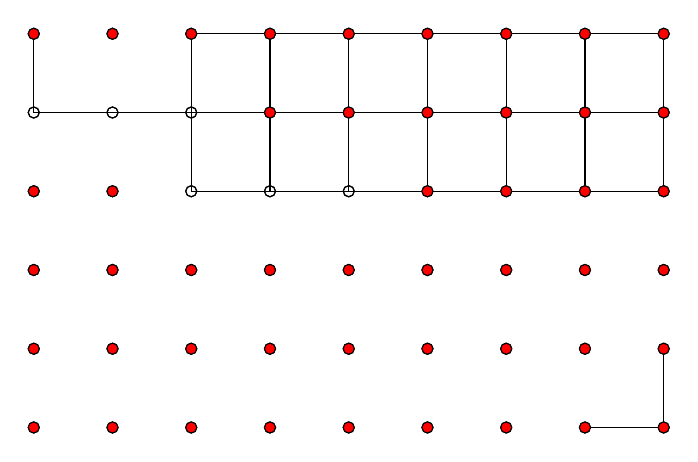
\begin{tikzpicture}[scale=1]%
\path[draw] (0.0,-8.0) -- (1.0,-8.0);%
\path[draw,radius=2pt] (0.0,-8.0) circle;%
\path[draw] (1.0,-8.0) -- (0.0,-8.0);%
\path[draw] (1.0,-8.0) -- (2.0,-8.0);%
\path[draw,radius=2pt] (1.0,-8.0) circle;%
\path[draw] (2.0,-8.0) -- (2.0,-9.0);%
\path[draw] (2.0,-8.0) -- (1.0,-8.0);%
\path[draw,radius=2pt] (2.0,-8.0) circle;%
\path[draw] (2.0,-9.0) -- (2.0,-8.0);%
\path[draw] (2.0,-9.0) -- (3.0,-9.0);%
\path[draw,radius=2pt] (2.0,-9.0) circle;%
\path[draw] (3.0,-9.0) -- (2.0,-9.0);%
\path[draw] (3.0,-9.0) -- (4.0,-9.0);%
\path[draw,radius=2pt] (3.0,-9.0) circle;%
\path[draw] (4.0,-9.0) -- (3.0,-9.0);%
\path[draw,radius=2pt] (4.0,-9.0) circle;%
\path[draw] (8.0,-11.0) -- (8.0,-12.0);%
\path[draw,radius=2pt] (8.0,-11.0) circle;%
\path[draw] (7.0,-12.0) -- (8.0,-12.0);%
\path[draw,radius=2pt] (7.0,-12.0) circle;%
\path[draw] (8.0,-12.0) -- (8.0,-11.0);%
\path[draw] (8.0,-12.0) -- (7.0,-12.0);%
\path[draw,radius=2pt] (8.0,-12.0) circle;%
\path[draw] (0.0,-7.0) -- (0.0,-8.0);%
\path[draw,radius=2pt] (0.0,-7.0) circle;%
\path[draw] (2.0,-7.0) -- (2.0,-8.0);%
\path[draw] (2.0,-7.0) -- (3.0,-7.0);%
\path[draw,radius=2pt] (2.0,-7.0) circle;%
\path[draw] (3.0,-7.0) -- (3.0,-8.0);%
\path[draw] (3.0,-7.0) -- (2.0,-7.0);%
\path[draw] (3.0,-7.0) -- (4.0,-7.0);%
\path[draw,radius=2pt] (3.0,-7.0) circle;%
\path[draw] (4.0,-7.0) -- (4.0,-8.0);%
\path[draw] (4.0,-7.0) -- (3.0,-7.0);%
\path[draw] (4.0,-7.0) -- (5.0,-7.0);%
\path[draw,radius=2pt] (4.0,-7.0) circle;%
\path[draw] (5.0,-7.0) -- (5.0,-8.0);%
\path[draw] (5.0,-7.0) -- (4.0,-7.0);%
\path[draw] (5.0,-7.0) -- (6.0,-7.0);%
\path[draw,radius=2pt] (5.0,-7.0) circle;%
\path[draw] (6.0,-7.0) -- (6.0,-8.0);%
\path[draw] (6.0,-7.0) -- (5.0,-7.0);%
\path[draw] (6.0,-7.0) -- (7.0,-7.0);%
\path[draw,radius=2pt] (6.0,-7.0) circle;%
\path[draw] (7.0,-7.0) -- (7.0,-8.0);%
\path[draw] (7.0,-7.0) -- (6.0,-7.0);%
\path[draw] (7.0,-7.0) -- (8.0,-7.0);%
\path[draw,radius=2pt] (7.0,-7.0) circle;%
\path[draw] (8.0,-7.0) -- (8.0,-8.0);%
\path[draw] (8.0,-7.0) -- (7.0,-7.0);%
\path[draw,radius=2pt] (8.0,-7.0) circle;%
\path[draw] (0.0,-8.0) -- (0.0,-7.0);%
\path[draw] (0.0,-8.0) -- (1.0,-8.0);%
\path[draw,radius=2pt] (0.0,-8.0) circle;%
\path[draw] (1.0,-8.0) -- (0.0,-8.0);%
\path[draw] (1.0,-8.0) -- (2.0,-8.0);%
\path[draw,radius=2pt] (1.0,-8.0) circle;%
\path[draw] (2.0,-8.0) -- (2.0,-7.0);%
\path[draw] (2.0,-8.0) -- (2.0,-9.0);%
\path[draw] (2.0,-8.0) -- (1.0,-8.0);%
\path[draw] (2.0,-8.0) -- (3.0,-8.0);%
\path[draw,radius=2pt] (2.0,-8.0) circle;%
\path[draw] (3.0,-8.0) -- (3.0,-7.0);%
\path[draw] (3.0,-8.0) -- (3.0,-9.0);%
\path[draw] (3.0,-8.0) -- (2.0,-8.0);%
\path[draw] (3.0,-8.0) -- (4.0,-8.0);%
\path[draw,radius=2pt] (3.0,-8.0) circle;%
\path[draw] (4.0,-8.0) -- (4.0,-7.0);%
\path[draw] (4.0,-8.0) -- (4.0,-9.0);%
\path[draw] (4.0,-8.0) -- (3.0,-8.0);%
\path[draw] (4.0,-8.0) -- (5.0,-8.0);%
\path[draw,radius=2pt] (4.0,-8.0) circle;%
\path[draw] (5.0,-8.0) -- (5.0,-7.0);%
\path[draw] (5.0,-8.0) -- (5.0,-9.0);%
\path[draw] (5.0,-8.0) -- (4.0,-8.0);%
\path[draw] (5.0,-8.0) -- (6.0,-8.0);%
\path[draw,radius=2pt] (5.0,-8.0) circle;%
\path[draw] (6.0,-8.0) -- (6.0,-7.0);%
\path[draw] (6.0,-8.0) -- (6.0,-9.0);%
\path[draw] (6.0,-8.0) -- (5.0,-8.0);%
\path[draw] (6.0,-8.0) -- (7.0,-8.0);%
\path[draw,radius=2pt] (6.0,-8.0) circle;%
\path[draw] (7.0,-8.0) -- (7.0,-7.0);%
\path[draw] (7.0,-8.0) -- (7.0,-9.0);%
\path[draw] (7.0,-8.0) -- (6.0,-8.0);%
\path[draw] (7.0,-8.0) -- (8.0,-8.0);%
\path[draw,radius=2pt] (7.0,-8.0) circle;%
\path[draw] (8.0,-8.0) -- (8.0,-7.0);%
\path[draw] (8.0,-8.0) -- (8.0,-9.0);%
\path[draw] (8.0,-8.0) -- (7.0,-8.0);%
\path[draw,radius=2pt] (8.0,-8.0) circle;%
\path[draw] (2.0,-9.0) -- (2.0,-8.0);%
\path[draw] (2.0,-9.0) -- (3.0,-9.0);%
\path[draw,radius=2pt] (2.0,-9.0) circle;%
\path[draw] (3.0,-9.0) -- (3.0,-8.0);%
\path[draw] (3.0,-9.0) -- (2.0,-9.0);%
\path[draw] (3.0,-9.0) -- (4.0,-9.0);%
\path[draw,radius=2pt] (3.0,-9.0) circle;%
\path[draw] (4.0,-9.0) -- (4.0,-8.0);%
\path[draw] (4.0,-9.0) -- (3.0,-9.0);%
\path[draw] (4.0,-9.0) -- (5.0,-9.0);%
\path[draw,radius=2pt] (4.0,-9.0) circle;%
\path[draw] (5.0,-9.0) -- (5.0,-8.0);%
\path[draw] (5.0,-9.0) -- (4.0,-9.0);%
\path[draw] (5.0,-9.0) -- (6.0,-9.0);%
\path[draw,radius=2pt] (5.0,-9.0) circle;%
\path[draw] (6.0,-9.0) -- (6.0,-8.0);%
\path[draw] (6.0,-9.0) -- (5.0,-9.0);%
\path[draw] (6.0,-9.0) -- (7.0,-9.0);%
\path[draw,radius=2pt] (6.0,-9.0) circle;%
\path[draw] (7.0,-9.0) -- (7.0,-8.0);%
\path[draw] (7.0,-9.0) -- (6.0,-9.0);%
\path[draw] (7.0,-9.0) -- (8.0,-9.0);%
\path[draw,radius=2pt] (7.0,-9.0) circle;%
\path[draw] (8.0,-9.0) -- (8.0,-8.0);%
\path[draw] (8.0,-9.0) -- (7.0,-9.0);%
\path[draw,radius=2pt] (8.0,-9.0) circle;%
\path[draw,radius=2pt,fill=red] (0.0,-7.0) circle;%
\path[draw,radius=2pt,fill=red] (1.0,-7.0) circle;%
\path[draw,radius=2pt,fill=red] (2.0,-7.0) circle;%
\path[draw,radius=2pt,fill=red] (3.0,-7.0) circle;%
\path[draw,radius=2pt,fill=red] (4.0,-7.0) circle;%
\path[draw,radius=2pt,fill=red] (5.0,-7.0) circle;%
\path[draw,radius=2pt,fill=red] (6.0,-7.0) circle;%
\path[draw,radius=2pt,fill=red] (7.0,-7.0) circle;%
\path[draw,radius=2pt,fill=red] (8.0,-7.0) circle;%
\path[draw,radius=2pt,fill=red] (3.0,-8.0) circle;%
\path[draw,radius=2pt,fill=red] (4.0,-8.0) circle;%
\path[draw,radius=2pt,fill=red] (5.0,-8.0) circle;%
\path[draw,radius=2pt,fill=red] (6.0,-8.0) circle;%
\path[draw,radius=2pt,fill=red] (7.0,-8.0) circle;%
\path[draw,radius=2pt,fill=red] (8.0,-8.0) circle;%
\path[draw,radius=2pt,fill=red] (0.0,-9.0) circle;%
\path[draw,radius=2pt,fill=red] (1.0,-9.0) circle;%
\path[draw,radius=2pt,fill=red] (5.0,-9.0) circle;%
\path[draw,radius=2pt,fill=red] (6.0,-9.0) circle;%
\path[draw,radius=2pt,fill=red] (7.0,-9.0) circle;%
\path[draw,radius=2pt,fill=red] (8.0,-9.0) circle;%
\path[draw,radius=2pt,fill=red] (0.0,-10.0) circle;%
\path[draw,radius=2pt,fill=red] (1.0,-10.0) circle;%
\path[draw,radius=2pt,fill=red] (2.0,-10.0) circle;%
\path[draw,radius=2pt,fill=red] (3.0,-10.0) circle;%
\path[draw,radius=2pt,fill=red] (4.0,-10.0) circle;%
\path[draw,radius=2pt,fill=red] (5.0,-10.0) circle;%
\path[draw,radius=2pt,fill=red] (6.0,-10.0) circle;%
\path[draw,radius=2pt,fill=red] (7.0,-10.0) circle;%
\path[draw,radius=2pt,fill=red] (8.0,-10.0) circle;%
\path[draw,radius=2pt,fill=red] (0.0,-11.0) circle;%
\path[draw,radius=2pt,fill=red] (1.0,-11.0) circle;%
\path[draw,radius=2pt,fill=red] (2.0,-11.0) circle;%
\path[draw,radius=2pt,fill=red] (3.0,-11.0) circle;%
\path[draw,radius=2pt,fill=red] (4.0,-11.0) circle;%
\path[draw,radius=2pt,fill=red] (5.0,-11.0) circle;%
\path[draw,radius=2pt,fill=red] (6.0,-11.0) circle;%
\path[draw,radius=2pt,fill=red] (7.0,-11.0) circle;%
\path[draw,radius=2pt,fill=red] (0.0,-12.0) circle;%
\path[draw,radius=2pt,fill=red] (1.0,-12.0) circle;%
\path[draw,radius=2pt,fill=red] (2.0,-12.0) circle;%
\path[draw,radius=2pt,fill=red] (3.0,-12.0) circle;%
\path[draw,radius=2pt,fill=red] (4.0,-12.0) circle;%
\path[draw,radius=2pt,fill=red] (5.0,-12.0) circle;%
\path[draw,radius=2pt,fill=red] (6.0,-12.0) circle;%
\path[draw,radius=2pt,fill=red] (1.0,-7.0) circle;%
\path[draw,radius=2pt,fill=red] (0.0,-9.0) circle;%
\path[draw,radius=2pt,fill=red] (1.0,-9.0) circle;%
\path[draw,radius=2pt,fill=red] (0.0,-10.0) circle;%
\path[draw,radius=2pt,fill=red] (1.0,-10.0) circle;%
\path[draw,radius=2pt,fill=red] (2.0,-10.0) circle;%
\path[draw,radius=2pt,fill=red] (3.0,-10.0) circle;%
\path[draw,radius=2pt,fill=red] (4.0,-10.0) circle;%
\path[draw,radius=2pt,fill=red] (5.0,-10.0) circle;%
\path[draw,radius=2pt,fill=red] (6.0,-10.0) circle;%
\path[draw,radius=2pt,fill=red] (7.0,-10.0) circle;%
\path[draw,radius=2pt,fill=red] (8.0,-10.0) circle;%
\path[draw,radius=2pt,fill=red] (0.0,-11.0) circle;%
\path[draw,radius=2pt,fill=red] (1.0,-11.0) circle;%
\path[draw,radius=2pt,fill=red] (2.0,-11.0) circle;%
\path[draw,radius=2pt,fill=red] (3.0,-11.0) circle;%
\path[draw,radius=2pt,fill=red] (4.0,-11.0) circle;%
\path[draw,radius=2pt,fill=red] (5.0,-11.0) circle;%
\path[draw,radius=2pt,fill=red] (6.0,-11.0) circle;%
\path[draw,radius=2pt,fill=red] (7.0,-11.0) circle;%
\path[draw,radius=2pt,fill=red] (8.0,-11.0) circle;%
\path[draw,radius=2pt,fill=red] (0.0,-12.0) circle;%
\path[draw,radius=2pt,fill=red] (1.0,-12.0) circle;%
\path[draw,radius=2pt,fill=red] (2.0,-12.0) circle;%
\path[draw,radius=2pt,fill=red] (3.0,-12.0) circle;%
\path[draw,radius=2pt,fill=red] (4.0,-12.0) circle;%
\path[draw,radius=2pt,fill=red] (5.0,-12.0) circle;%
\path[draw,radius=2pt,fill=red] (6.0,-12.0) circle;%
\path[draw,radius=2pt,fill=red] (7.0,-12.0) circle;%
\path[draw,radius=2pt,fill=red] (8.0,-12.0) circle;%
\end{tikzpicture}%
\newline%
\hspace*{1in}%
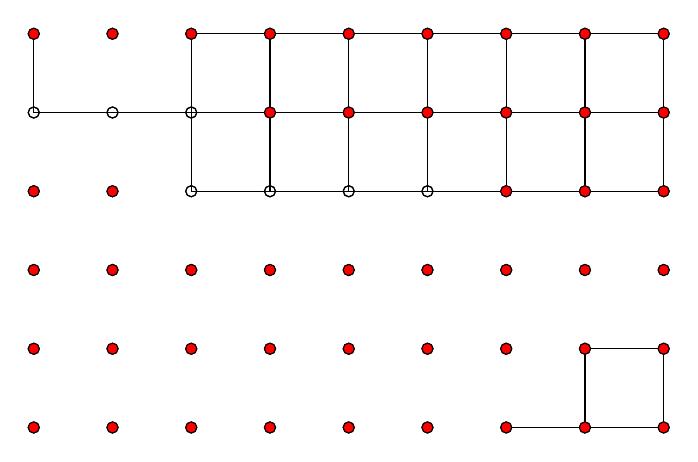
\begin{tikzpicture}[scale=1]%
\path[draw] (0.0,-8.0) -- (1.0,-8.0);%
\path[draw,radius=2pt] (0.0,-8.0) circle;%
\path[draw] (1.0,-8.0) -- (0.0,-8.0);%
\path[draw] (1.0,-8.0) -- (2.0,-8.0);%
\path[draw,radius=2pt] (1.0,-8.0) circle;%
\path[draw] (2.0,-8.0) -- (2.0,-9.0);%
\path[draw] (2.0,-8.0) -- (1.0,-8.0);%
\path[draw,radius=2pt] (2.0,-8.0) circle;%
\path[draw] (2.0,-9.0) -- (2.0,-8.0);%
\path[draw] (2.0,-9.0) -- (3.0,-9.0);%
\path[draw,radius=2pt] (2.0,-9.0) circle;%
\path[draw] (3.0,-9.0) -- (2.0,-9.0);%
\path[draw] (3.0,-9.0) -- (4.0,-9.0);%
\path[draw,radius=2pt] (3.0,-9.0) circle;%
\path[draw] (4.0,-9.0) -- (3.0,-9.0);%
\path[draw] (4.0,-9.0) -- (5.0,-9.0);%
\path[draw,radius=2pt] (4.0,-9.0) circle;%
\path[draw] (5.0,-9.0) -- (4.0,-9.0);%
\path[draw,radius=2pt] (5.0,-9.0) circle;%
\path[draw] (7.0,-11.0) -- (7.0,-12.0);%
\path[draw] (7.0,-11.0) -- (8.0,-11.0);%
\path[draw,radius=2pt] (7.0,-11.0) circle;%
\path[draw] (8.0,-11.0) -- (8.0,-12.0);%
\path[draw] (8.0,-11.0) -- (7.0,-11.0);%
\path[draw,radius=2pt] (8.0,-11.0) circle;%
\path[draw] (6.0,-12.0) -- (7.0,-12.0);%
\path[draw,radius=2pt] (6.0,-12.0) circle;%
\path[draw] (7.0,-12.0) -- (7.0,-11.0);%
\path[draw] (7.0,-12.0) -- (6.0,-12.0);%
\path[draw] (7.0,-12.0) -- (8.0,-12.0);%
\path[draw,radius=2pt] (7.0,-12.0) circle;%
\path[draw] (8.0,-12.0) -- (8.0,-11.0);%
\path[draw] (8.0,-12.0) -- (7.0,-12.0);%
\path[draw,radius=2pt] (8.0,-12.0) circle;%
\path[draw] (0.0,-7.0) -- (0.0,-8.0);%
\path[draw,radius=2pt] (0.0,-7.0) circle;%
\path[draw] (2.0,-7.0) -- (2.0,-8.0);%
\path[draw] (2.0,-7.0) -- (3.0,-7.0);%
\path[draw,radius=2pt] (2.0,-7.0) circle;%
\path[draw] (3.0,-7.0) -- (3.0,-8.0);%
\path[draw] (3.0,-7.0) -- (2.0,-7.0);%
\path[draw] (3.0,-7.0) -- (4.0,-7.0);%
\path[draw,radius=2pt] (3.0,-7.0) circle;%
\path[draw] (4.0,-7.0) -- (4.0,-8.0);%
\path[draw] (4.0,-7.0) -- (3.0,-7.0);%
\path[draw] (4.0,-7.0) -- (5.0,-7.0);%
\path[draw,radius=2pt] (4.0,-7.0) circle;%
\path[draw] (5.0,-7.0) -- (5.0,-8.0);%
\path[draw] (5.0,-7.0) -- (4.0,-7.0);%
\path[draw] (5.0,-7.0) -- (6.0,-7.0);%
\path[draw,radius=2pt] (5.0,-7.0) circle;%
\path[draw] (6.0,-7.0) -- (6.0,-8.0);%
\path[draw] (6.0,-7.0) -- (5.0,-7.0);%
\path[draw] (6.0,-7.0) -- (7.0,-7.0);%
\path[draw,radius=2pt] (6.0,-7.0) circle;%
\path[draw] (7.0,-7.0) -- (7.0,-8.0);%
\path[draw] (7.0,-7.0) -- (6.0,-7.0);%
\path[draw] (7.0,-7.0) -- (8.0,-7.0);%
\path[draw,radius=2pt] (7.0,-7.0) circle;%
\path[draw] (8.0,-7.0) -- (8.0,-8.0);%
\path[draw] (8.0,-7.0) -- (7.0,-7.0);%
\path[draw,radius=2pt] (8.0,-7.0) circle;%
\path[draw] (0.0,-8.0) -- (0.0,-7.0);%
\path[draw] (0.0,-8.0) -- (1.0,-8.0);%
\path[draw,radius=2pt] (0.0,-8.0) circle;%
\path[draw] (1.0,-8.0) -- (0.0,-8.0);%
\path[draw] (1.0,-8.0) -- (2.0,-8.0);%
\path[draw,radius=2pt] (1.0,-8.0) circle;%
\path[draw] (2.0,-8.0) -- (2.0,-7.0);%
\path[draw] (2.0,-8.0) -- (2.0,-9.0);%
\path[draw] (2.0,-8.0) -- (1.0,-8.0);%
\path[draw] (2.0,-8.0) -- (3.0,-8.0);%
\path[draw,radius=2pt] (2.0,-8.0) circle;%
\path[draw] (3.0,-8.0) -- (3.0,-7.0);%
\path[draw] (3.0,-8.0) -- (3.0,-9.0);%
\path[draw] (3.0,-8.0) -- (2.0,-8.0);%
\path[draw] (3.0,-8.0) -- (4.0,-8.0);%
\path[draw,radius=2pt] (3.0,-8.0) circle;%
\path[draw] (4.0,-8.0) -- (4.0,-7.0);%
\path[draw] (4.0,-8.0) -- (4.0,-9.0);%
\path[draw] (4.0,-8.0) -- (3.0,-8.0);%
\path[draw] (4.0,-8.0) -- (5.0,-8.0);%
\path[draw,radius=2pt] (4.0,-8.0) circle;%
\path[draw] (5.0,-8.0) -- (5.0,-7.0);%
\path[draw] (5.0,-8.0) -- (5.0,-9.0);%
\path[draw] (5.0,-8.0) -- (4.0,-8.0);%
\path[draw] (5.0,-8.0) -- (6.0,-8.0);%
\path[draw,radius=2pt] (5.0,-8.0) circle;%
\path[draw] (6.0,-8.0) -- (6.0,-7.0);%
\path[draw] (6.0,-8.0) -- (6.0,-9.0);%
\path[draw] (6.0,-8.0) -- (5.0,-8.0);%
\path[draw] (6.0,-8.0) -- (7.0,-8.0);%
\path[draw,radius=2pt] (6.0,-8.0) circle;%
\path[draw] (7.0,-8.0) -- (7.0,-7.0);%
\path[draw] (7.0,-8.0) -- (7.0,-9.0);%
\path[draw] (7.0,-8.0) -- (6.0,-8.0);%
\path[draw] (7.0,-8.0) -- (8.0,-8.0);%
\path[draw,radius=2pt] (7.0,-8.0) circle;%
\path[draw] (8.0,-8.0) -- (8.0,-7.0);%
\path[draw] (8.0,-8.0) -- (8.0,-9.0);%
\path[draw] (8.0,-8.0) -- (7.0,-8.0);%
\path[draw,radius=2pt] (8.0,-8.0) circle;%
\path[draw] (2.0,-9.0) -- (2.0,-8.0);%
\path[draw] (2.0,-9.0) -- (3.0,-9.0);%
\path[draw,radius=2pt] (2.0,-9.0) circle;%
\path[draw] (3.0,-9.0) -- (3.0,-8.0);%
\path[draw] (3.0,-9.0) -- (2.0,-9.0);%
\path[draw] (3.0,-9.0) -- (4.0,-9.0);%
\path[draw,radius=2pt] (3.0,-9.0) circle;%
\path[draw] (4.0,-9.0) -- (4.0,-8.0);%
\path[draw] (4.0,-9.0) -- (3.0,-9.0);%
\path[draw] (4.0,-9.0) -- (5.0,-9.0);%
\path[draw,radius=2pt] (4.0,-9.0) circle;%
\path[draw] (5.0,-9.0) -- (5.0,-8.0);%
\path[draw] (5.0,-9.0) -- (4.0,-9.0);%
\path[draw] (5.0,-9.0) -- (6.0,-9.0);%
\path[draw,radius=2pt] (5.0,-9.0) circle;%
\path[draw] (6.0,-9.0) -- (6.0,-8.0);%
\path[draw] (6.0,-9.0) -- (5.0,-9.0);%
\path[draw] (6.0,-9.0) -- (7.0,-9.0);%
\path[draw,radius=2pt] (6.0,-9.0) circle;%
\path[draw] (7.0,-9.0) -- (7.0,-8.0);%
\path[draw] (7.0,-9.0) -- (6.0,-9.0);%
\path[draw] (7.0,-9.0) -- (8.0,-9.0);%
\path[draw,radius=2pt] (7.0,-9.0) circle;%
\path[draw] (8.0,-9.0) -- (8.0,-8.0);%
\path[draw] (8.0,-9.0) -- (7.0,-9.0);%
\path[draw,radius=2pt] (8.0,-9.0) circle;%
\path[draw,radius=2pt,fill=red] (0.0,-7.0) circle;%
\path[draw,radius=2pt,fill=red] (1.0,-7.0) circle;%
\path[draw,radius=2pt,fill=red] (2.0,-7.0) circle;%
\path[draw,radius=2pt,fill=red] (3.0,-7.0) circle;%
\path[draw,radius=2pt,fill=red] (4.0,-7.0) circle;%
\path[draw,radius=2pt,fill=red] (5.0,-7.0) circle;%
\path[draw,radius=2pt,fill=red] (6.0,-7.0) circle;%
\path[draw,radius=2pt,fill=red] (7.0,-7.0) circle;%
\path[draw,radius=2pt,fill=red] (8.0,-7.0) circle;%
\path[draw,radius=2pt,fill=red] (3.0,-8.0) circle;%
\path[draw,radius=2pt,fill=red] (4.0,-8.0) circle;%
\path[draw,radius=2pt,fill=red] (5.0,-8.0) circle;%
\path[draw,radius=2pt,fill=red] (6.0,-8.0) circle;%
\path[draw,radius=2pt,fill=red] (7.0,-8.0) circle;%
\path[draw,radius=2pt,fill=red] (8.0,-8.0) circle;%
\path[draw,radius=2pt,fill=red] (0.0,-9.0) circle;%
\path[draw,radius=2pt,fill=red] (1.0,-9.0) circle;%
\path[draw,radius=2pt,fill=red] (6.0,-9.0) circle;%
\path[draw,radius=2pt,fill=red] (7.0,-9.0) circle;%
\path[draw,radius=2pt,fill=red] (8.0,-9.0) circle;%
\path[draw,radius=2pt,fill=red] (0.0,-10.0) circle;%
\path[draw,radius=2pt,fill=red] (1.0,-10.0) circle;%
\path[draw,radius=2pt,fill=red] (2.0,-10.0) circle;%
\path[draw,radius=2pt,fill=red] (3.0,-10.0) circle;%
\path[draw,radius=2pt,fill=red] (4.0,-10.0) circle;%
\path[draw,radius=2pt,fill=red] (5.0,-10.0) circle;%
\path[draw,radius=2pt,fill=red] (6.0,-10.0) circle;%
\path[draw,radius=2pt,fill=red] (7.0,-10.0) circle;%
\path[draw,radius=2pt,fill=red] (8.0,-10.0) circle;%
\path[draw,radius=2pt,fill=red] (0.0,-11.0) circle;%
\path[draw,radius=2pt,fill=red] (1.0,-11.0) circle;%
\path[draw,radius=2pt,fill=red] (2.0,-11.0) circle;%
\path[draw,radius=2pt,fill=red] (3.0,-11.0) circle;%
\path[draw,radius=2pt,fill=red] (4.0,-11.0) circle;%
\path[draw,radius=2pt,fill=red] (5.0,-11.0) circle;%
\path[draw,radius=2pt,fill=red] (6.0,-11.0) circle;%
\path[draw,radius=2pt,fill=red] (0.0,-12.0) circle;%
\path[draw,radius=2pt,fill=red] (1.0,-12.0) circle;%
\path[draw,radius=2pt,fill=red] (2.0,-12.0) circle;%
\path[draw,radius=2pt,fill=red] (3.0,-12.0) circle;%
\path[draw,radius=2pt,fill=red] (4.0,-12.0) circle;%
\path[draw,radius=2pt,fill=red] (5.0,-12.0) circle;%
\path[draw,radius=2pt,fill=red] (1.0,-7.0) circle;%
\path[draw,radius=2pt,fill=red] (0.0,-9.0) circle;%
\path[draw,radius=2pt,fill=red] (1.0,-9.0) circle;%
\path[draw,radius=2pt,fill=red] (0.0,-10.0) circle;%
\path[draw,radius=2pt,fill=red] (1.0,-10.0) circle;%
\path[draw,radius=2pt,fill=red] (2.0,-10.0) circle;%
\path[draw,radius=2pt,fill=red] (3.0,-10.0) circle;%
\path[draw,radius=2pt,fill=red] (4.0,-10.0) circle;%
\path[draw,radius=2pt,fill=red] (5.0,-10.0) circle;%
\path[draw,radius=2pt,fill=red] (6.0,-10.0) circle;%
\path[draw,radius=2pt,fill=red] (7.0,-10.0) circle;%
\path[draw,radius=2pt,fill=red] (8.0,-10.0) circle;%
\path[draw,radius=2pt,fill=red] (0.0,-11.0) circle;%
\path[draw,radius=2pt,fill=red] (1.0,-11.0) circle;%
\path[draw,radius=2pt,fill=red] (2.0,-11.0) circle;%
\path[draw,radius=2pt,fill=red] (3.0,-11.0) circle;%
\path[draw,radius=2pt,fill=red] (4.0,-11.0) circle;%
\path[draw,radius=2pt,fill=red] (5.0,-11.0) circle;%
\path[draw,radius=2pt,fill=red] (6.0,-11.0) circle;%
\path[draw,radius=2pt,fill=red] (7.0,-11.0) circle;%
\path[draw,radius=2pt,fill=red] (8.0,-11.0) circle;%
\path[draw,radius=2pt,fill=red] (0.0,-12.0) circle;%
\path[draw,radius=2pt,fill=red] (1.0,-12.0) circle;%
\path[draw,radius=2pt,fill=red] (2.0,-12.0) circle;%
\path[draw,radius=2pt,fill=red] (3.0,-12.0) circle;%
\path[draw,radius=2pt,fill=red] (4.0,-12.0) circle;%
\path[draw,radius=2pt,fill=red] (5.0,-12.0) circle;%
\path[draw,radius=2pt,fill=red] (6.0,-12.0) circle;%
\path[draw,radius=2pt,fill=red] (7.0,-12.0) circle;%
\path[draw,radius=2pt,fill=red] (8.0,-12.0) circle;%
\end{tikzpicture}%
\hspace*{1in}%
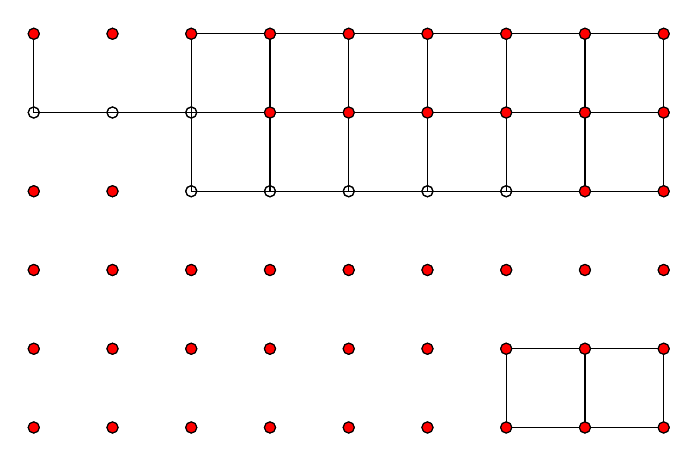
\begin{tikzpicture}[scale=1]%
\path[draw] (0.0,-8.0) -- (1.0,-8.0);%
\path[draw,radius=2pt] (0.0,-8.0) circle;%
\path[draw] (1.0,-8.0) -- (0.0,-8.0);%
\path[draw] (1.0,-8.0) -- (2.0,-8.0);%
\path[draw,radius=2pt] (1.0,-8.0) circle;%
\path[draw] (2.0,-8.0) -- (2.0,-9.0);%
\path[draw] (2.0,-8.0) -- (1.0,-8.0);%
\path[draw,radius=2pt] (2.0,-8.0) circle;%
\path[draw] (2.0,-9.0) -- (2.0,-8.0);%
\path[draw] (2.0,-9.0) -- (3.0,-9.0);%
\path[draw,radius=2pt] (2.0,-9.0) circle;%
\path[draw] (3.0,-9.0) -- (2.0,-9.0);%
\path[draw] (3.0,-9.0) -- (4.0,-9.0);%
\path[draw,radius=2pt] (3.0,-9.0) circle;%
\path[draw] (4.0,-9.0) -- (3.0,-9.0);%
\path[draw] (4.0,-9.0) -- (5.0,-9.0);%
\path[draw,radius=2pt] (4.0,-9.0) circle;%
\path[draw] (5.0,-9.0) -- (4.0,-9.0);%
\path[draw] (5.0,-9.0) -- (6.0,-9.0);%
\path[draw,radius=2pt] (5.0,-9.0) circle;%
\path[draw] (6.0,-9.0) -- (5.0,-9.0);%
\path[draw,radius=2pt] (6.0,-9.0) circle;%
\path[draw] (6.0,-11.0) -- (6.0,-12.0);%
\path[draw] (6.0,-11.0) -- (7.0,-11.0);%
\path[draw,radius=2pt] (6.0,-11.0) circle;%
\path[draw] (7.0,-11.0) -- (7.0,-12.0);%
\path[draw] (7.0,-11.0) -- (6.0,-11.0);%
\path[draw] (7.0,-11.0) -- (8.0,-11.0);%
\path[draw,radius=2pt] (7.0,-11.0) circle;%
\path[draw] (8.0,-11.0) -- (8.0,-12.0);%
\path[draw] (8.0,-11.0) -- (7.0,-11.0);%
\path[draw,radius=2pt] (8.0,-11.0) circle;%
\path[draw] (6.0,-12.0) -- (6.0,-11.0);%
\path[draw] (6.0,-12.0) -- (7.0,-12.0);%
\path[draw,radius=2pt] (6.0,-12.0) circle;%
\path[draw] (7.0,-12.0) -- (7.0,-11.0);%
\path[draw] (7.0,-12.0) -- (6.0,-12.0);%
\path[draw] (7.0,-12.0) -- (8.0,-12.0);%
\path[draw,radius=2pt] (7.0,-12.0) circle;%
\path[draw] (8.0,-12.0) -- (8.0,-11.0);%
\path[draw] (8.0,-12.0) -- (7.0,-12.0);%
\path[draw,radius=2pt] (8.0,-12.0) circle;%
\path[draw] (0.0,-7.0) -- (0.0,-8.0);%
\path[draw,radius=2pt] (0.0,-7.0) circle;%
\path[draw] (2.0,-7.0) -- (2.0,-8.0);%
\path[draw] (2.0,-7.0) -- (3.0,-7.0);%
\path[draw,radius=2pt] (2.0,-7.0) circle;%
\path[draw] (3.0,-7.0) -- (3.0,-8.0);%
\path[draw] (3.0,-7.0) -- (2.0,-7.0);%
\path[draw] (3.0,-7.0) -- (4.0,-7.0);%
\path[draw,radius=2pt] (3.0,-7.0) circle;%
\path[draw] (4.0,-7.0) -- (4.0,-8.0);%
\path[draw] (4.0,-7.0) -- (3.0,-7.0);%
\path[draw] (4.0,-7.0) -- (5.0,-7.0);%
\path[draw,radius=2pt] (4.0,-7.0) circle;%
\path[draw] (5.0,-7.0) -- (5.0,-8.0);%
\path[draw] (5.0,-7.0) -- (4.0,-7.0);%
\path[draw] (5.0,-7.0) -- (6.0,-7.0);%
\path[draw,radius=2pt] (5.0,-7.0) circle;%
\path[draw] (6.0,-7.0) -- (6.0,-8.0);%
\path[draw] (6.0,-7.0) -- (5.0,-7.0);%
\path[draw] (6.0,-7.0) -- (7.0,-7.0);%
\path[draw,radius=2pt] (6.0,-7.0) circle;%
\path[draw] (7.0,-7.0) -- (7.0,-8.0);%
\path[draw] (7.0,-7.0) -- (6.0,-7.0);%
\path[draw] (7.0,-7.0) -- (8.0,-7.0);%
\path[draw,radius=2pt] (7.0,-7.0) circle;%
\path[draw] (8.0,-7.0) -- (8.0,-8.0);%
\path[draw] (8.0,-7.0) -- (7.0,-7.0);%
\path[draw,radius=2pt] (8.0,-7.0) circle;%
\path[draw] (0.0,-8.0) -- (0.0,-7.0);%
\path[draw] (0.0,-8.0) -- (1.0,-8.0);%
\path[draw,radius=2pt] (0.0,-8.0) circle;%
\path[draw] (1.0,-8.0) -- (0.0,-8.0);%
\path[draw] (1.0,-8.0) -- (2.0,-8.0);%
\path[draw,radius=2pt] (1.0,-8.0) circle;%
\path[draw] (2.0,-8.0) -- (2.0,-7.0);%
\path[draw] (2.0,-8.0) -- (2.0,-9.0);%
\path[draw] (2.0,-8.0) -- (1.0,-8.0);%
\path[draw] (2.0,-8.0) -- (3.0,-8.0);%
\path[draw,radius=2pt] (2.0,-8.0) circle;%
\path[draw] (3.0,-8.0) -- (3.0,-7.0);%
\path[draw] (3.0,-8.0) -- (3.0,-9.0);%
\path[draw] (3.0,-8.0) -- (2.0,-8.0);%
\path[draw] (3.0,-8.0) -- (4.0,-8.0);%
\path[draw,radius=2pt] (3.0,-8.0) circle;%
\path[draw] (4.0,-8.0) -- (4.0,-7.0);%
\path[draw] (4.0,-8.0) -- (4.0,-9.0);%
\path[draw] (4.0,-8.0) -- (3.0,-8.0);%
\path[draw] (4.0,-8.0) -- (5.0,-8.0);%
\path[draw,radius=2pt] (4.0,-8.0) circle;%
\path[draw] (5.0,-8.0) -- (5.0,-7.0);%
\path[draw] (5.0,-8.0) -- (5.0,-9.0);%
\path[draw] (5.0,-8.0) -- (4.0,-8.0);%
\path[draw] (5.0,-8.0) -- (6.0,-8.0);%
\path[draw,radius=2pt] (5.0,-8.0) circle;%
\path[draw] (6.0,-8.0) -- (6.0,-7.0);%
\path[draw] (6.0,-8.0) -- (6.0,-9.0);%
\path[draw] (6.0,-8.0) -- (5.0,-8.0);%
\path[draw] (6.0,-8.0) -- (7.0,-8.0);%
\path[draw,radius=2pt] (6.0,-8.0) circle;%
\path[draw] (7.0,-8.0) -- (7.0,-7.0);%
\path[draw] (7.0,-8.0) -- (7.0,-9.0);%
\path[draw] (7.0,-8.0) -- (6.0,-8.0);%
\path[draw] (7.0,-8.0) -- (8.0,-8.0);%
\path[draw,radius=2pt] (7.0,-8.0) circle;%
\path[draw] (8.0,-8.0) -- (8.0,-7.0);%
\path[draw] (8.0,-8.0) -- (8.0,-9.0);%
\path[draw] (8.0,-8.0) -- (7.0,-8.0);%
\path[draw,radius=2pt] (8.0,-8.0) circle;%
\path[draw] (2.0,-9.0) -- (2.0,-8.0);%
\path[draw] (2.0,-9.0) -- (3.0,-9.0);%
\path[draw,radius=2pt] (2.0,-9.0) circle;%
\path[draw] (3.0,-9.0) -- (3.0,-8.0);%
\path[draw] (3.0,-9.0) -- (2.0,-9.0);%
\path[draw] (3.0,-9.0) -- (4.0,-9.0);%
\path[draw,radius=2pt] (3.0,-9.0) circle;%
\path[draw] (4.0,-9.0) -- (4.0,-8.0);%
\path[draw] (4.0,-9.0) -- (3.0,-9.0);%
\path[draw] (4.0,-9.0) -- (5.0,-9.0);%
\path[draw,radius=2pt] (4.0,-9.0) circle;%
\path[draw] (5.0,-9.0) -- (5.0,-8.0);%
\path[draw] (5.0,-9.0) -- (4.0,-9.0);%
\path[draw] (5.0,-9.0) -- (6.0,-9.0);%
\path[draw,radius=2pt] (5.0,-9.0) circle;%
\path[draw] (6.0,-9.0) -- (6.0,-8.0);%
\path[draw] (6.0,-9.0) -- (5.0,-9.0);%
\path[draw] (6.0,-9.0) -- (7.0,-9.0);%
\path[draw,radius=2pt] (6.0,-9.0) circle;%
\path[draw] (7.0,-9.0) -- (7.0,-8.0);%
\path[draw] (7.0,-9.0) -- (6.0,-9.0);%
\path[draw] (7.0,-9.0) -- (8.0,-9.0);%
\path[draw,radius=2pt] (7.0,-9.0) circle;%
\path[draw] (8.0,-9.0) -- (8.0,-8.0);%
\path[draw] (8.0,-9.0) -- (7.0,-9.0);%
\path[draw,radius=2pt] (8.0,-9.0) circle;%
\path[draw,radius=2pt,fill=red] (0.0,-7.0) circle;%
\path[draw,radius=2pt,fill=red] (1.0,-7.0) circle;%
\path[draw,radius=2pt,fill=red] (2.0,-7.0) circle;%
\path[draw,radius=2pt,fill=red] (3.0,-7.0) circle;%
\path[draw,radius=2pt,fill=red] (4.0,-7.0) circle;%
\path[draw,radius=2pt,fill=red] (5.0,-7.0) circle;%
\path[draw,radius=2pt,fill=red] (6.0,-7.0) circle;%
\path[draw,radius=2pt,fill=red] (7.0,-7.0) circle;%
\path[draw,radius=2pt,fill=red] (8.0,-7.0) circle;%
\path[draw,radius=2pt,fill=red] (3.0,-8.0) circle;%
\path[draw,radius=2pt,fill=red] (4.0,-8.0) circle;%
\path[draw,radius=2pt,fill=red] (5.0,-8.0) circle;%
\path[draw,radius=2pt,fill=red] (6.0,-8.0) circle;%
\path[draw,radius=2pt,fill=red] (7.0,-8.0) circle;%
\path[draw,radius=2pt,fill=red] (8.0,-8.0) circle;%
\path[draw,radius=2pt,fill=red] (0.0,-9.0) circle;%
\path[draw,radius=2pt,fill=red] (1.0,-9.0) circle;%
\path[draw,radius=2pt,fill=red] (7.0,-9.0) circle;%
\path[draw,radius=2pt,fill=red] (8.0,-9.0) circle;%
\path[draw,radius=2pt,fill=red] (0.0,-10.0) circle;%
\path[draw,radius=2pt,fill=red] (1.0,-10.0) circle;%
\path[draw,radius=2pt,fill=red] (2.0,-10.0) circle;%
\path[draw,radius=2pt,fill=red] (3.0,-10.0) circle;%
\path[draw,radius=2pt,fill=red] (4.0,-10.0) circle;%
\path[draw,radius=2pt,fill=red] (5.0,-10.0) circle;%
\path[draw,radius=2pt,fill=red] (6.0,-10.0) circle;%
\path[draw,radius=2pt,fill=red] (7.0,-10.0) circle;%
\path[draw,radius=2pt,fill=red] (8.0,-10.0) circle;%
\path[draw,radius=2pt,fill=red] (0.0,-11.0) circle;%
\path[draw,radius=2pt,fill=red] (1.0,-11.0) circle;%
\path[draw,radius=2pt,fill=red] (2.0,-11.0) circle;%
\path[draw,radius=2pt,fill=red] (3.0,-11.0) circle;%
\path[draw,radius=2pt,fill=red] (4.0,-11.0) circle;%
\path[draw,radius=2pt,fill=red] (5.0,-11.0) circle;%
\path[draw,radius=2pt,fill=red] (0.0,-12.0) circle;%
\path[draw,radius=2pt,fill=red] (1.0,-12.0) circle;%
\path[draw,radius=2pt,fill=red] (2.0,-12.0) circle;%
\path[draw,radius=2pt,fill=red] (3.0,-12.0) circle;%
\path[draw,radius=2pt,fill=red] (4.0,-12.0) circle;%
\path[draw,radius=2pt,fill=red] (5.0,-12.0) circle;%
\path[draw,radius=2pt,fill=red] (1.0,-7.0) circle;%
\path[draw,radius=2pt,fill=red] (0.0,-9.0) circle;%
\path[draw,radius=2pt,fill=red] (1.0,-9.0) circle;%
\path[draw,radius=2pt,fill=red] (0.0,-10.0) circle;%
\path[draw,radius=2pt,fill=red] (1.0,-10.0) circle;%
\path[draw,radius=2pt,fill=red] (2.0,-10.0) circle;%
\path[draw,radius=2pt,fill=red] (3.0,-10.0) circle;%
\path[draw,radius=2pt,fill=red] (4.0,-10.0) circle;%
\path[draw,radius=2pt,fill=red] (5.0,-10.0) circle;%
\path[draw,radius=2pt,fill=red] (6.0,-10.0) circle;%
\path[draw,radius=2pt,fill=red] (7.0,-10.0) circle;%
\path[draw,radius=2pt,fill=red] (8.0,-10.0) circle;%
\path[draw,radius=2pt,fill=red] (0.0,-11.0) circle;%
\path[draw,radius=2pt,fill=red] (1.0,-11.0) circle;%
\path[draw,radius=2pt,fill=red] (2.0,-11.0) circle;%
\path[draw,radius=2pt,fill=red] (3.0,-11.0) circle;%
\path[draw,radius=2pt,fill=red] (4.0,-11.0) circle;%
\path[draw,radius=2pt,fill=red] (5.0,-11.0) circle;%
\path[draw,radius=2pt,fill=red] (6.0,-11.0) circle;%
\path[draw,radius=2pt,fill=red] (7.0,-11.0) circle;%
\path[draw,radius=2pt,fill=red] (8.0,-11.0) circle;%
\path[draw,radius=2pt,fill=red] (0.0,-12.0) circle;%
\path[draw,radius=2pt,fill=red] (1.0,-12.0) circle;%
\path[draw,radius=2pt,fill=red] (2.0,-12.0) circle;%
\path[draw,radius=2pt,fill=red] (3.0,-12.0) circle;%
\path[draw,radius=2pt,fill=red] (4.0,-12.0) circle;%
\path[draw,radius=2pt,fill=red] (5.0,-12.0) circle;%
\path[draw,radius=2pt,fill=red] (6.0,-12.0) circle;%
\path[draw,radius=2pt,fill=red] (7.0,-12.0) circle;%
\path[draw,radius=2pt,fill=red] (8.0,-12.0) circle;%
\end{tikzpicture}%
\hspace*{1in}%
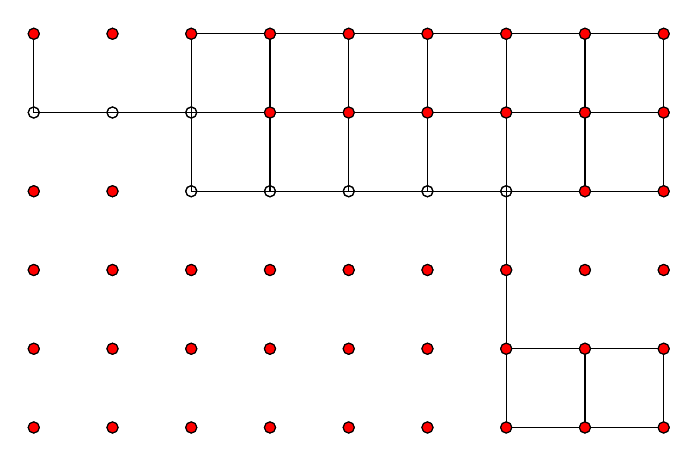
\begin{tikzpicture}[scale=1]%
\path[draw] (0.0,-8.0) -- (1.0,-8.0);%
\path[draw,radius=2pt] (0.0,-8.0) circle;%
\path[draw] (1.0,-8.0) -- (0.0,-8.0);%
\path[draw] (1.0,-8.0) -- (2.0,-8.0);%
\path[draw,radius=2pt] (1.0,-8.0) circle;%
\path[draw] (2.0,-8.0) -- (2.0,-9.0);%
\path[draw] (2.0,-8.0) -- (1.0,-8.0);%
\path[draw,radius=2pt] (2.0,-8.0) circle;%
\path[draw] (2.0,-9.0) -- (2.0,-8.0);%
\path[draw] (2.0,-9.0) -- (3.0,-9.0);%
\path[draw,radius=2pt] (2.0,-9.0) circle;%
\path[draw] (3.0,-9.0) -- (2.0,-9.0);%
\path[draw] (3.0,-9.0) -- (4.0,-9.0);%
\path[draw,radius=2pt] (3.0,-9.0) circle;%
\path[draw] (4.0,-9.0) -- (3.0,-9.0);%
\path[draw] (4.0,-9.0) -- (5.0,-9.0);%
\path[draw,radius=2pt] (4.0,-9.0) circle;%
\path[draw] (5.0,-9.0) -- (4.0,-9.0);%
\path[draw] (5.0,-9.0) -- (6.0,-9.0);%
\path[draw,radius=2pt] (5.0,-9.0) circle;%
\path[draw] (6.0,-9.0) -- (6.0,-10.0);%
\path[draw] (6.0,-9.0) -- (5.0,-9.0);%
\path[draw,radius=2pt] (6.0,-9.0) circle;%
\path[draw] (6.0,-10.0) -- (6.0,-9.0);%
\path[draw] (6.0,-10.0) -- (6.0,-11.0);%
\path[draw,radius=2pt] (6.0,-10.0) circle;%
\path[draw] (6.0,-11.0) -- (6.0,-10.0);%
\path[draw] (6.0,-11.0) -- (6.0,-12.0);%
\path[draw] (6.0,-11.0) -- (7.0,-11.0);%
\path[draw,radius=2pt] (6.0,-11.0) circle;%
\path[draw] (7.0,-11.0) -- (7.0,-12.0);%
\path[draw] (7.0,-11.0) -- (6.0,-11.0);%
\path[draw] (7.0,-11.0) -- (8.0,-11.0);%
\path[draw,radius=2pt] (7.0,-11.0) circle;%
\path[draw] (8.0,-11.0) -- (8.0,-12.0);%
\path[draw] (8.0,-11.0) -- (7.0,-11.0);%
\path[draw,radius=2pt] (8.0,-11.0) circle;%
\path[draw] (6.0,-12.0) -- (6.0,-11.0);%
\path[draw] (6.0,-12.0) -- (7.0,-12.0);%
\path[draw,radius=2pt] (6.0,-12.0) circle;%
\path[draw] (7.0,-12.0) -- (7.0,-11.0);%
\path[draw] (7.0,-12.0) -- (6.0,-12.0);%
\path[draw] (7.0,-12.0) -- (8.0,-12.0);%
\path[draw,radius=2pt] (7.0,-12.0) circle;%
\path[draw] (8.0,-12.0) -- (8.0,-11.0);%
\path[draw] (8.0,-12.0) -- (7.0,-12.0);%
\path[draw,radius=2pt] (8.0,-12.0) circle;%
\path[draw] (0.0,-7.0) -- (0.0,-8.0);%
\path[draw,radius=2pt] (0.0,-7.0) circle;%
\path[draw] (2.0,-7.0) -- (2.0,-8.0);%
\path[draw] (2.0,-7.0) -- (3.0,-7.0);%
\path[draw,radius=2pt] (2.0,-7.0) circle;%
\path[draw] (3.0,-7.0) -- (3.0,-8.0);%
\path[draw] (3.0,-7.0) -- (2.0,-7.0);%
\path[draw] (3.0,-7.0) -- (4.0,-7.0);%
\path[draw,radius=2pt] (3.0,-7.0) circle;%
\path[draw] (4.0,-7.0) -- (4.0,-8.0);%
\path[draw] (4.0,-7.0) -- (3.0,-7.0);%
\path[draw] (4.0,-7.0) -- (5.0,-7.0);%
\path[draw,radius=2pt] (4.0,-7.0) circle;%
\path[draw] (5.0,-7.0) -- (5.0,-8.0);%
\path[draw] (5.0,-7.0) -- (4.0,-7.0);%
\path[draw] (5.0,-7.0) -- (6.0,-7.0);%
\path[draw,radius=2pt] (5.0,-7.0) circle;%
\path[draw] (6.0,-7.0) -- (6.0,-8.0);%
\path[draw] (6.0,-7.0) -- (5.0,-7.0);%
\path[draw] (6.0,-7.0) -- (7.0,-7.0);%
\path[draw,radius=2pt] (6.0,-7.0) circle;%
\path[draw] (7.0,-7.0) -- (7.0,-8.0);%
\path[draw] (7.0,-7.0) -- (6.0,-7.0);%
\path[draw] (7.0,-7.0) -- (8.0,-7.0);%
\path[draw,radius=2pt] (7.0,-7.0) circle;%
\path[draw] (8.0,-7.0) -- (8.0,-8.0);%
\path[draw] (8.0,-7.0) -- (7.0,-7.0);%
\path[draw,radius=2pt] (8.0,-7.0) circle;%
\path[draw] (0.0,-8.0) -- (0.0,-7.0);%
\path[draw] (0.0,-8.0) -- (1.0,-8.0);%
\path[draw,radius=2pt] (0.0,-8.0) circle;%
\path[draw] (1.0,-8.0) -- (0.0,-8.0);%
\path[draw] (1.0,-8.0) -- (2.0,-8.0);%
\path[draw,radius=2pt] (1.0,-8.0) circle;%
\path[draw] (2.0,-8.0) -- (2.0,-7.0);%
\path[draw] (2.0,-8.0) -- (2.0,-9.0);%
\path[draw] (2.0,-8.0) -- (1.0,-8.0);%
\path[draw] (2.0,-8.0) -- (3.0,-8.0);%
\path[draw,radius=2pt] (2.0,-8.0) circle;%
\path[draw] (3.0,-8.0) -- (3.0,-7.0);%
\path[draw] (3.0,-8.0) -- (3.0,-9.0);%
\path[draw] (3.0,-8.0) -- (2.0,-8.0);%
\path[draw] (3.0,-8.0) -- (4.0,-8.0);%
\path[draw,radius=2pt] (3.0,-8.0) circle;%
\path[draw] (4.0,-8.0) -- (4.0,-7.0);%
\path[draw] (4.0,-8.0) -- (4.0,-9.0);%
\path[draw] (4.0,-8.0) -- (3.0,-8.0);%
\path[draw] (4.0,-8.0) -- (5.0,-8.0);%
\path[draw,radius=2pt] (4.0,-8.0) circle;%
\path[draw] (5.0,-8.0) -- (5.0,-7.0);%
\path[draw] (5.0,-8.0) -- (5.0,-9.0);%
\path[draw] (5.0,-8.0) -- (4.0,-8.0);%
\path[draw] (5.0,-8.0) -- (6.0,-8.0);%
\path[draw,radius=2pt] (5.0,-8.0) circle;%
\path[draw] (6.0,-8.0) -- (6.0,-7.0);%
\path[draw] (6.0,-8.0) -- (6.0,-9.0);%
\path[draw] (6.0,-8.0) -- (5.0,-8.0);%
\path[draw] (6.0,-8.0) -- (7.0,-8.0);%
\path[draw,radius=2pt] (6.0,-8.0) circle;%
\path[draw] (7.0,-8.0) -- (7.0,-7.0);%
\path[draw] (7.0,-8.0) -- (7.0,-9.0);%
\path[draw] (7.0,-8.0) -- (6.0,-8.0);%
\path[draw] (7.0,-8.0) -- (8.0,-8.0);%
\path[draw,radius=2pt] (7.0,-8.0) circle;%
\path[draw] (8.0,-8.0) -- (8.0,-7.0);%
\path[draw] (8.0,-8.0) -- (8.0,-9.0);%
\path[draw] (8.0,-8.0) -- (7.0,-8.0);%
\path[draw,radius=2pt] (8.0,-8.0) circle;%
\path[draw] (2.0,-9.0) -- (2.0,-8.0);%
\path[draw] (2.0,-9.0) -- (3.0,-9.0);%
\path[draw,radius=2pt] (2.0,-9.0) circle;%
\path[draw] (3.0,-9.0) -- (3.0,-8.0);%
\path[draw] (3.0,-9.0) -- (2.0,-9.0);%
\path[draw] (3.0,-9.0) -- (4.0,-9.0);%
\path[draw,radius=2pt] (3.0,-9.0) circle;%
\path[draw] (4.0,-9.0) -- (4.0,-8.0);%
\path[draw] (4.0,-9.0) -- (3.0,-9.0);%
\path[draw] (4.0,-9.0) -- (5.0,-9.0);%
\path[draw,radius=2pt] (4.0,-9.0) circle;%
\path[draw] (5.0,-9.0) -- (5.0,-8.0);%
\path[draw] (5.0,-9.0) -- (4.0,-9.0);%
\path[draw] (5.0,-9.0) -- (6.0,-9.0);%
\path[draw,radius=2pt] (5.0,-9.0) circle;%
\path[draw] (6.0,-9.0) -- (6.0,-8.0);%
\path[draw] (6.0,-9.0) -- (5.0,-9.0);%
\path[draw] (6.0,-9.0) -- (7.0,-9.0);%
\path[draw,radius=2pt] (6.0,-9.0) circle;%
\path[draw] (7.0,-9.0) -- (7.0,-8.0);%
\path[draw] (7.0,-9.0) -- (6.0,-9.0);%
\path[draw] (7.0,-9.0) -- (8.0,-9.0);%
\path[draw,radius=2pt] (7.0,-9.0) circle;%
\path[draw] (8.0,-9.0) -- (8.0,-8.0);%
\path[draw] (8.0,-9.0) -- (7.0,-9.0);%
\path[draw,radius=2pt] (8.0,-9.0) circle;%
\path[draw,radius=2pt,fill=red] (0.0,-7.0) circle;%
\path[draw,radius=2pt,fill=red] (1.0,-7.0) circle;%
\path[draw,radius=2pt,fill=red] (2.0,-7.0) circle;%
\path[draw,radius=2pt,fill=red] (3.0,-7.0) circle;%
\path[draw,radius=2pt,fill=red] (4.0,-7.0) circle;%
\path[draw,radius=2pt,fill=red] (5.0,-7.0) circle;%
\path[draw,radius=2pt,fill=red] (6.0,-7.0) circle;%
\path[draw,radius=2pt,fill=red] (7.0,-7.0) circle;%
\path[draw,radius=2pt,fill=red] (8.0,-7.0) circle;%
\path[draw,radius=2pt,fill=red] (3.0,-8.0) circle;%
\path[draw,radius=2pt,fill=red] (4.0,-8.0) circle;%
\path[draw,radius=2pt,fill=red] (5.0,-8.0) circle;%
\path[draw,radius=2pt,fill=red] (6.0,-8.0) circle;%
\path[draw,radius=2pt,fill=red] (7.0,-8.0) circle;%
\path[draw,radius=2pt,fill=red] (8.0,-8.0) circle;%
\path[draw,radius=2pt,fill=red] (0.0,-9.0) circle;%
\path[draw,radius=2pt,fill=red] (1.0,-9.0) circle;%
\path[draw,radius=2pt,fill=red] (7.0,-9.0) circle;%
\path[draw,radius=2pt,fill=red] (8.0,-9.0) circle;%
\path[draw,radius=2pt,fill=red] (0.0,-10.0) circle;%
\path[draw,radius=2pt,fill=red] (1.0,-10.0) circle;%
\path[draw,radius=2pt,fill=red] (2.0,-10.0) circle;%
\path[draw,radius=2pt,fill=red] (3.0,-10.0) circle;%
\path[draw,radius=2pt,fill=red] (4.0,-10.0) circle;%
\path[draw,radius=2pt,fill=red] (5.0,-10.0) circle;%
\path[draw,radius=2pt,fill=red] (7.0,-10.0) circle;%
\path[draw,radius=2pt,fill=red] (8.0,-10.0) circle;%
\path[draw,radius=2pt,fill=red] (0.0,-11.0) circle;%
\path[draw,radius=2pt,fill=red] (1.0,-11.0) circle;%
\path[draw,radius=2pt,fill=red] (2.0,-11.0) circle;%
\path[draw,radius=2pt,fill=red] (3.0,-11.0) circle;%
\path[draw,radius=2pt,fill=red] (4.0,-11.0) circle;%
\path[draw,radius=2pt,fill=red] (5.0,-11.0) circle;%
\path[draw,radius=2pt,fill=red] (0.0,-12.0) circle;%
\path[draw,radius=2pt,fill=red] (1.0,-12.0) circle;%
\path[draw,radius=2pt,fill=red] (2.0,-12.0) circle;%
\path[draw,radius=2pt,fill=red] (3.0,-12.0) circle;%
\path[draw,radius=2pt,fill=red] (4.0,-12.0) circle;%
\path[draw,radius=2pt,fill=red] (5.0,-12.0) circle;%
\path[draw,radius=2pt,fill=red] (1.0,-7.0) circle;%
\path[draw,radius=2pt,fill=red] (0.0,-9.0) circle;%
\path[draw,radius=2pt,fill=red] (1.0,-9.0) circle;%
\path[draw,radius=2pt,fill=red] (0.0,-10.0) circle;%
\path[draw,radius=2pt,fill=red] (1.0,-10.0) circle;%
\path[draw,radius=2pt,fill=red] (2.0,-10.0) circle;%
\path[draw,radius=2pt,fill=red] (3.0,-10.0) circle;%
\path[draw,radius=2pt,fill=red] (4.0,-10.0) circle;%
\path[draw,radius=2pt,fill=red] (5.0,-10.0) circle;%
\path[draw,radius=2pt,fill=red] (6.0,-10.0) circle;%
\path[draw,radius=2pt,fill=red] (7.0,-10.0) circle;%
\path[draw,radius=2pt,fill=red] (8.0,-10.0) circle;%
\path[draw,radius=2pt,fill=red] (0.0,-11.0) circle;%
\path[draw,radius=2pt,fill=red] (1.0,-11.0) circle;%
\path[draw,radius=2pt,fill=red] (2.0,-11.0) circle;%
\path[draw,radius=2pt,fill=red] (3.0,-11.0) circle;%
\path[draw,radius=2pt,fill=red] (4.0,-11.0) circle;%
\path[draw,radius=2pt,fill=red] (5.0,-11.0) circle;%
\path[draw,radius=2pt,fill=red] (6.0,-11.0) circle;%
\path[draw,radius=2pt,fill=red] (7.0,-11.0) circle;%
\path[draw,radius=2pt,fill=red] (8.0,-11.0) circle;%
\path[draw,radius=2pt,fill=red] (0.0,-12.0) circle;%
\path[draw,radius=2pt,fill=red] (1.0,-12.0) circle;%
\path[draw,radius=2pt,fill=red] (2.0,-12.0) circle;%
\path[draw,radius=2pt,fill=red] (3.0,-12.0) circle;%
\path[draw,radius=2pt,fill=red] (4.0,-12.0) circle;%
\path[draw,radius=2pt,fill=red] (5.0,-12.0) circle;%
\path[draw,radius=2pt,fill=red] (6.0,-12.0) circle;%
\path[draw,radius=2pt,fill=red] (7.0,-12.0) circle;%
\path[draw,radius=2pt,fill=red] (8.0,-12.0) circle;%
\end{tikzpicture}%
\newline%
\hspace*{1in}%
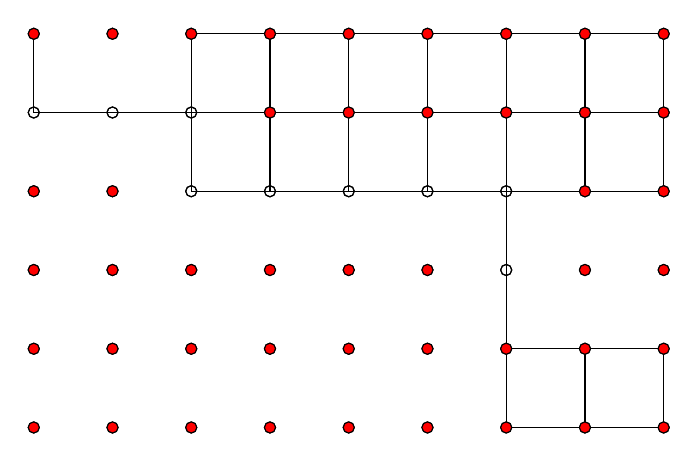
\begin{tikzpicture}[scale=1]%
\path[draw] (0.0,-8.0) -- (1.0,-8.0);%
\path[draw,radius=2pt] (0.0,-8.0) circle;%
\path[draw] (1.0,-8.0) -- (0.0,-8.0);%
\path[draw] (1.0,-8.0) -- (2.0,-8.0);%
\path[draw,radius=2pt] (1.0,-8.0) circle;%
\path[draw] (2.0,-8.0) -- (2.0,-9.0);%
\path[draw] (2.0,-8.0) -- (1.0,-8.0);%
\path[draw,radius=2pt] (2.0,-8.0) circle;%
\path[draw] (2.0,-9.0) -- (2.0,-8.0);%
\path[draw] (2.0,-9.0) -- (3.0,-9.0);%
\path[draw,radius=2pt] (2.0,-9.0) circle;%
\path[draw] (3.0,-9.0) -- (2.0,-9.0);%
\path[draw] (3.0,-9.0) -- (4.0,-9.0);%
\path[draw,radius=2pt] (3.0,-9.0) circle;%
\path[draw] (4.0,-9.0) -- (3.0,-9.0);%
\path[draw] (4.0,-9.0) -- (5.0,-9.0);%
\path[draw,radius=2pt] (4.0,-9.0) circle;%
\path[draw] (5.0,-9.0) -- (4.0,-9.0);%
\path[draw] (5.0,-9.0) -- (6.0,-9.0);%
\path[draw,radius=2pt] (5.0,-9.0) circle;%
\path[draw] (6.0,-9.0) -- (6.0,-10.0);%
\path[draw] (6.0,-9.0) -- (5.0,-9.0);%
\path[draw,radius=2pt] (6.0,-9.0) circle;%
\path[draw] (6.0,-10.0) -- (6.0,-9.0);%
\path[draw] (6.0,-10.0) -- (6.0,-11.0);%
\path[draw,radius=2pt] (6.0,-10.0) circle;%
\path[draw] (6.0,-11.0) -- (6.0,-10.0);%
\path[draw] (6.0,-11.0) -- (6.0,-12.0);%
\path[draw] (6.0,-11.0) -- (7.0,-11.0);%
\path[draw,radius=2pt] (6.0,-11.0) circle;%
\path[draw] (7.0,-11.0) -- (7.0,-12.0);%
\path[draw] (7.0,-11.0) -- (6.0,-11.0);%
\path[draw] (7.0,-11.0) -- (8.0,-11.0);%
\path[draw,radius=2pt] (7.0,-11.0) circle;%
\path[draw] (8.0,-11.0) -- (8.0,-12.0);%
\path[draw] (8.0,-11.0) -- (7.0,-11.0);%
\path[draw,radius=2pt] (8.0,-11.0) circle;%
\path[draw] (6.0,-12.0) -- (6.0,-11.0);%
\path[draw] (6.0,-12.0) -- (7.0,-12.0);%
\path[draw,radius=2pt] (6.0,-12.0) circle;%
\path[draw] (7.0,-12.0) -- (7.0,-11.0);%
\path[draw] (7.0,-12.0) -- (6.0,-12.0);%
\path[draw] (7.0,-12.0) -- (8.0,-12.0);%
\path[draw,radius=2pt] (7.0,-12.0) circle;%
\path[draw] (8.0,-12.0) -- (8.0,-11.0);%
\path[draw] (8.0,-12.0) -- (7.0,-12.0);%
\path[draw,radius=2pt] (8.0,-12.0) circle;%
\path[draw] (0.0,-7.0) -- (0.0,-8.0);%
\path[draw,radius=2pt] (0.0,-7.0) circle;%
\path[draw] (2.0,-7.0) -- (2.0,-8.0);%
\path[draw] (2.0,-7.0) -- (3.0,-7.0);%
\path[draw,radius=2pt] (2.0,-7.0) circle;%
\path[draw] (3.0,-7.0) -- (3.0,-8.0);%
\path[draw] (3.0,-7.0) -- (2.0,-7.0);%
\path[draw] (3.0,-7.0) -- (4.0,-7.0);%
\path[draw,radius=2pt] (3.0,-7.0) circle;%
\path[draw] (4.0,-7.0) -- (4.0,-8.0);%
\path[draw] (4.0,-7.0) -- (3.0,-7.0);%
\path[draw] (4.0,-7.0) -- (5.0,-7.0);%
\path[draw,radius=2pt] (4.0,-7.0) circle;%
\path[draw] (5.0,-7.0) -- (5.0,-8.0);%
\path[draw] (5.0,-7.0) -- (4.0,-7.0);%
\path[draw] (5.0,-7.0) -- (6.0,-7.0);%
\path[draw,radius=2pt] (5.0,-7.0) circle;%
\path[draw] (6.0,-7.0) -- (6.0,-8.0);%
\path[draw] (6.0,-7.0) -- (5.0,-7.0);%
\path[draw] (6.0,-7.0) -- (7.0,-7.0);%
\path[draw,radius=2pt] (6.0,-7.0) circle;%
\path[draw] (7.0,-7.0) -- (7.0,-8.0);%
\path[draw] (7.0,-7.0) -- (6.0,-7.0);%
\path[draw] (7.0,-7.0) -- (8.0,-7.0);%
\path[draw,radius=2pt] (7.0,-7.0) circle;%
\path[draw] (8.0,-7.0) -- (8.0,-8.0);%
\path[draw] (8.0,-7.0) -- (7.0,-7.0);%
\path[draw,radius=2pt] (8.0,-7.0) circle;%
\path[draw] (0.0,-8.0) -- (0.0,-7.0);%
\path[draw] (0.0,-8.0) -- (1.0,-8.0);%
\path[draw,radius=2pt] (0.0,-8.0) circle;%
\path[draw] (1.0,-8.0) -- (0.0,-8.0);%
\path[draw] (1.0,-8.0) -- (2.0,-8.0);%
\path[draw,radius=2pt] (1.0,-8.0) circle;%
\path[draw] (2.0,-8.0) -- (2.0,-7.0);%
\path[draw] (2.0,-8.0) -- (2.0,-9.0);%
\path[draw] (2.0,-8.0) -- (1.0,-8.0);%
\path[draw] (2.0,-8.0) -- (3.0,-8.0);%
\path[draw,radius=2pt] (2.0,-8.0) circle;%
\path[draw] (3.0,-8.0) -- (3.0,-7.0);%
\path[draw] (3.0,-8.0) -- (3.0,-9.0);%
\path[draw] (3.0,-8.0) -- (2.0,-8.0);%
\path[draw] (3.0,-8.0) -- (4.0,-8.0);%
\path[draw,radius=2pt] (3.0,-8.0) circle;%
\path[draw] (4.0,-8.0) -- (4.0,-7.0);%
\path[draw] (4.0,-8.0) -- (4.0,-9.0);%
\path[draw] (4.0,-8.0) -- (3.0,-8.0);%
\path[draw] (4.0,-8.0) -- (5.0,-8.0);%
\path[draw,radius=2pt] (4.0,-8.0) circle;%
\path[draw] (5.0,-8.0) -- (5.0,-7.0);%
\path[draw] (5.0,-8.0) -- (5.0,-9.0);%
\path[draw] (5.0,-8.0) -- (4.0,-8.0);%
\path[draw] (5.0,-8.0) -- (6.0,-8.0);%
\path[draw,radius=2pt] (5.0,-8.0) circle;%
\path[draw] (6.0,-8.0) -- (6.0,-7.0);%
\path[draw] (6.0,-8.0) -- (6.0,-9.0);%
\path[draw] (6.0,-8.0) -- (5.0,-8.0);%
\path[draw] (6.0,-8.0) -- (7.0,-8.0);%
\path[draw,radius=2pt] (6.0,-8.0) circle;%
\path[draw] (7.0,-8.0) -- (7.0,-7.0);%
\path[draw] (7.0,-8.0) -- (7.0,-9.0);%
\path[draw] (7.0,-8.0) -- (6.0,-8.0);%
\path[draw] (7.0,-8.0) -- (8.0,-8.0);%
\path[draw,radius=2pt] (7.0,-8.0) circle;%
\path[draw] (8.0,-8.0) -- (8.0,-7.0);%
\path[draw] (8.0,-8.0) -- (8.0,-9.0);%
\path[draw] (8.0,-8.0) -- (7.0,-8.0);%
\path[draw,radius=2pt] (8.0,-8.0) circle;%
\path[draw] (2.0,-9.0) -- (2.0,-8.0);%
\path[draw] (2.0,-9.0) -- (3.0,-9.0);%
\path[draw,radius=2pt] (2.0,-9.0) circle;%
\path[draw] (3.0,-9.0) -- (3.0,-8.0);%
\path[draw] (3.0,-9.0) -- (2.0,-9.0);%
\path[draw] (3.0,-9.0) -- (4.0,-9.0);%
\path[draw,radius=2pt] (3.0,-9.0) circle;%
\path[draw] (4.0,-9.0) -- (4.0,-8.0);%
\path[draw] (4.0,-9.0) -- (3.0,-9.0);%
\path[draw] (4.0,-9.0) -- (5.0,-9.0);%
\path[draw,radius=2pt] (4.0,-9.0) circle;%
\path[draw] (5.0,-9.0) -- (5.0,-8.0);%
\path[draw] (5.0,-9.0) -- (4.0,-9.0);%
\path[draw] (5.0,-9.0) -- (6.0,-9.0);%
\path[draw,radius=2pt] (5.0,-9.0) circle;%
\path[draw] (6.0,-9.0) -- (6.0,-8.0);%
\path[draw] (6.0,-9.0) -- (6.0,-10.0);%
\path[draw] (6.0,-9.0) -- (5.0,-9.0);%
\path[draw] (6.0,-9.0) -- (7.0,-9.0);%
\path[draw,radius=2pt] (6.0,-9.0) circle;%
\path[draw] (7.0,-9.0) -- (7.0,-8.0);%
\path[draw] (7.0,-9.0) -- (6.0,-9.0);%
\path[draw] (7.0,-9.0) -- (8.0,-9.0);%
\path[draw,radius=2pt] (7.0,-9.0) circle;%
\path[draw] (8.0,-9.0) -- (8.0,-8.0);%
\path[draw] (8.0,-9.0) -- (7.0,-9.0);%
\path[draw,radius=2pt] (8.0,-9.0) circle;%
\path[draw] (6.0,-10.0) -- (6.0,-9.0);%
\path[draw,radius=2pt] (6.0,-10.0) circle;%
\path[draw,radius=2pt,fill=red] (0.0,-7.0) circle;%
\path[draw,radius=2pt,fill=red] (1.0,-7.0) circle;%
\path[draw,radius=2pt,fill=red] (2.0,-7.0) circle;%
\path[draw,radius=2pt,fill=red] (3.0,-7.0) circle;%
\path[draw,radius=2pt,fill=red] (4.0,-7.0) circle;%
\path[draw,radius=2pt,fill=red] (5.0,-7.0) circle;%
\path[draw,radius=2pt,fill=red] (6.0,-7.0) circle;%
\path[draw,radius=2pt,fill=red] (7.0,-7.0) circle;%
\path[draw,radius=2pt,fill=red] (8.0,-7.0) circle;%
\path[draw,radius=2pt,fill=red] (3.0,-8.0) circle;%
\path[draw,radius=2pt,fill=red] (4.0,-8.0) circle;%
\path[draw,radius=2pt,fill=red] (5.0,-8.0) circle;%
\path[draw,radius=2pt,fill=red] (6.0,-8.0) circle;%
\path[draw,radius=2pt,fill=red] (7.0,-8.0) circle;%
\path[draw,radius=2pt,fill=red] (8.0,-8.0) circle;%
\path[draw,radius=2pt,fill=red] (0.0,-9.0) circle;%
\path[draw,radius=2pt,fill=red] (1.0,-9.0) circle;%
\path[draw,radius=2pt,fill=red] (7.0,-9.0) circle;%
\path[draw,radius=2pt,fill=red] (8.0,-9.0) circle;%
\path[draw,radius=2pt,fill=red] (0.0,-10.0) circle;%
\path[draw,radius=2pt,fill=red] (1.0,-10.0) circle;%
\path[draw,radius=2pt,fill=red] (2.0,-10.0) circle;%
\path[draw,radius=2pt,fill=red] (3.0,-10.0) circle;%
\path[draw,radius=2pt,fill=red] (4.0,-10.0) circle;%
\path[draw,radius=2pt,fill=red] (5.0,-10.0) circle;%
\path[draw,radius=2pt,fill=red] (7.0,-10.0) circle;%
\path[draw,radius=2pt,fill=red] (8.0,-10.0) circle;%
\path[draw,radius=2pt,fill=red] (0.0,-11.0) circle;%
\path[draw,radius=2pt,fill=red] (1.0,-11.0) circle;%
\path[draw,radius=2pt,fill=red] (2.0,-11.0) circle;%
\path[draw,radius=2pt,fill=red] (3.0,-11.0) circle;%
\path[draw,radius=2pt,fill=red] (4.0,-11.0) circle;%
\path[draw,radius=2pt,fill=red] (5.0,-11.0) circle;%
\path[draw,radius=2pt,fill=red] (0.0,-12.0) circle;%
\path[draw,radius=2pt,fill=red] (1.0,-12.0) circle;%
\path[draw,radius=2pt,fill=red] (2.0,-12.0) circle;%
\path[draw,radius=2pt,fill=red] (3.0,-12.0) circle;%
\path[draw,radius=2pt,fill=red] (4.0,-12.0) circle;%
\path[draw,radius=2pt,fill=red] (5.0,-12.0) circle;%
\path[draw,radius=2pt,fill=red] (1.0,-7.0) circle;%
\path[draw,radius=2pt,fill=red] (0.0,-9.0) circle;%
\path[draw,radius=2pt,fill=red] (1.0,-9.0) circle;%
\path[draw,radius=2pt,fill=red] (0.0,-10.0) circle;%
\path[draw,radius=2pt,fill=red] (1.0,-10.0) circle;%
\path[draw,radius=2pt,fill=red] (2.0,-10.0) circle;%
\path[draw,radius=2pt,fill=red] (3.0,-10.0) circle;%
\path[draw,radius=2pt,fill=red] (4.0,-10.0) circle;%
\path[draw,radius=2pt,fill=red] (5.0,-10.0) circle;%
\path[draw,radius=2pt,fill=red] (7.0,-10.0) circle;%
\path[draw,radius=2pt,fill=red] (8.0,-10.0) circle;%
\path[draw,radius=2pt,fill=red] (0.0,-11.0) circle;%
\path[draw,radius=2pt,fill=red] (1.0,-11.0) circle;%
\path[draw,radius=2pt,fill=red] (2.0,-11.0) circle;%
\path[draw,radius=2pt,fill=red] (3.0,-11.0) circle;%
\path[draw,radius=2pt,fill=red] (4.0,-11.0) circle;%
\path[draw,radius=2pt,fill=red] (5.0,-11.0) circle;%
\path[draw,radius=2pt,fill=red] (6.0,-11.0) circle;%
\path[draw,radius=2pt,fill=red] (7.0,-11.0) circle;%
\path[draw,radius=2pt,fill=red] (8.0,-11.0) circle;%
\path[draw,radius=2pt,fill=red] (0.0,-12.0) circle;%
\path[draw,radius=2pt,fill=red] (1.0,-12.0) circle;%
\path[draw,radius=2pt,fill=red] (2.0,-12.0) circle;%
\path[draw,radius=2pt,fill=red] (3.0,-12.0) circle;%
\path[draw,radius=2pt,fill=red] (4.0,-12.0) circle;%
\path[draw,radius=2pt,fill=red] (5.0,-12.0) circle;%
\path[draw,radius=2pt,fill=red] (6.0,-12.0) circle;%
\path[draw,radius=2pt,fill=red] (7.0,-12.0) circle;%
\path[draw,radius=2pt,fill=red] (8.0,-12.0) circle;%
\end{tikzpicture}%
\hspace*{1in}%
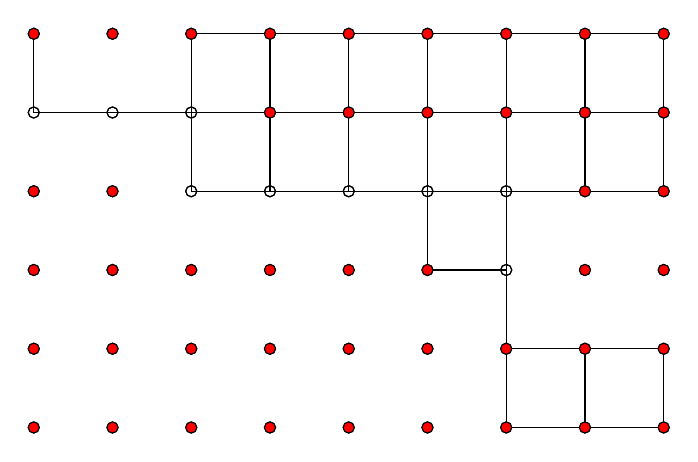
\begin{tikzpicture}[scale=1]%
\path[draw] (0.0,-8.0) -- (1.0,-8.0);%
\path[draw,radius=2pt] (0.0,-8.0) circle;%
\path[draw] (1.0,-8.0) -- (0.0,-8.0);%
\path[draw] (1.0,-8.0) -- (2.0,-8.0);%
\path[draw,radius=2pt] (1.0,-8.0) circle;%
\path[draw] (2.0,-8.0) -- (2.0,-9.0);%
\path[draw] (2.0,-8.0) -- (1.0,-8.0);%
\path[draw,radius=2pt] (2.0,-8.0) circle;%
\path[draw] (2.0,-9.0) -- (2.0,-8.0);%
\path[draw] (2.0,-9.0) -- (3.0,-9.0);%
\path[draw,radius=2pt] (2.0,-9.0) circle;%
\path[draw] (3.0,-9.0) -- (2.0,-9.0);%
\path[draw] (3.0,-9.0) -- (4.0,-9.0);%
\path[draw,radius=2pt] (3.0,-9.0) circle;%
\path[draw] (4.0,-9.0) -- (3.0,-9.0);%
\path[draw] (4.0,-9.0) -- (5.0,-9.0);%
\path[draw,radius=2pt] (4.0,-9.0) circle;%
\path[draw] (5.0,-9.0) -- (4.0,-9.0);%
\path[draw] (5.0,-9.0) -- (6.0,-9.0);%
\path[draw,radius=2pt] (5.0,-9.0) circle;%
\path[draw] (6.0,-9.0) -- (6.0,-10.0);%
\path[draw] (6.0,-9.0) -- (5.0,-9.0);%
\path[draw,radius=2pt] (6.0,-9.0) circle;%
\path[draw] (6.0,-10.0) -- (6.0,-9.0);%
\path[draw] (6.0,-10.0) -- (6.0,-11.0);%
\path[draw,radius=2pt] (6.0,-10.0) circle;%
\path[draw] (6.0,-11.0) -- (6.0,-10.0);%
\path[draw] (6.0,-11.0) -- (6.0,-12.0);%
\path[draw] (6.0,-11.0) -- (7.0,-11.0);%
\path[draw,radius=2pt] (6.0,-11.0) circle;%
\path[draw] (7.0,-11.0) -- (7.0,-12.0);%
\path[draw] (7.0,-11.0) -- (6.0,-11.0);%
\path[draw] (7.0,-11.0) -- (8.0,-11.0);%
\path[draw,radius=2pt] (7.0,-11.0) circle;%
\path[draw] (8.0,-11.0) -- (8.0,-12.0);%
\path[draw] (8.0,-11.0) -- (7.0,-11.0);%
\path[draw,radius=2pt] (8.0,-11.0) circle;%
\path[draw] (6.0,-12.0) -- (6.0,-11.0);%
\path[draw] (6.0,-12.0) -- (7.0,-12.0);%
\path[draw,radius=2pt] (6.0,-12.0) circle;%
\path[draw] (7.0,-12.0) -- (7.0,-11.0);%
\path[draw] (7.0,-12.0) -- (6.0,-12.0);%
\path[draw] (7.0,-12.0) -- (8.0,-12.0);%
\path[draw,radius=2pt] (7.0,-12.0) circle;%
\path[draw] (8.0,-12.0) -- (8.0,-11.0);%
\path[draw] (8.0,-12.0) -- (7.0,-12.0);%
\path[draw,radius=2pt] (8.0,-12.0) circle;%
\path[draw] (0.0,-7.0) -- (0.0,-8.0);%
\path[draw,radius=2pt] (0.0,-7.0) circle;%
\path[draw] (2.0,-7.0) -- (2.0,-8.0);%
\path[draw] (2.0,-7.0) -- (3.0,-7.0);%
\path[draw,radius=2pt] (2.0,-7.0) circle;%
\path[draw] (3.0,-7.0) -- (3.0,-8.0);%
\path[draw] (3.0,-7.0) -- (2.0,-7.0);%
\path[draw] (3.0,-7.0) -- (4.0,-7.0);%
\path[draw,radius=2pt] (3.0,-7.0) circle;%
\path[draw] (4.0,-7.0) -- (4.0,-8.0);%
\path[draw] (4.0,-7.0) -- (3.0,-7.0);%
\path[draw] (4.0,-7.0) -- (5.0,-7.0);%
\path[draw,radius=2pt] (4.0,-7.0) circle;%
\path[draw] (5.0,-7.0) -- (5.0,-8.0);%
\path[draw] (5.0,-7.0) -- (4.0,-7.0);%
\path[draw] (5.0,-7.0) -- (6.0,-7.0);%
\path[draw,radius=2pt] (5.0,-7.0) circle;%
\path[draw] (6.0,-7.0) -- (6.0,-8.0);%
\path[draw] (6.0,-7.0) -- (5.0,-7.0);%
\path[draw] (6.0,-7.0) -- (7.0,-7.0);%
\path[draw,radius=2pt] (6.0,-7.0) circle;%
\path[draw] (7.0,-7.0) -- (7.0,-8.0);%
\path[draw] (7.0,-7.0) -- (6.0,-7.0);%
\path[draw] (7.0,-7.0) -- (8.0,-7.0);%
\path[draw,radius=2pt] (7.0,-7.0) circle;%
\path[draw] (8.0,-7.0) -- (8.0,-8.0);%
\path[draw] (8.0,-7.0) -- (7.0,-7.0);%
\path[draw,radius=2pt] (8.0,-7.0) circle;%
\path[draw] (0.0,-8.0) -- (0.0,-7.0);%
\path[draw] (0.0,-8.0) -- (1.0,-8.0);%
\path[draw,radius=2pt] (0.0,-8.0) circle;%
\path[draw] (1.0,-8.0) -- (0.0,-8.0);%
\path[draw] (1.0,-8.0) -- (2.0,-8.0);%
\path[draw,radius=2pt] (1.0,-8.0) circle;%
\path[draw] (2.0,-8.0) -- (2.0,-7.0);%
\path[draw] (2.0,-8.0) -- (2.0,-9.0);%
\path[draw] (2.0,-8.0) -- (1.0,-8.0);%
\path[draw] (2.0,-8.0) -- (3.0,-8.0);%
\path[draw,radius=2pt] (2.0,-8.0) circle;%
\path[draw] (3.0,-8.0) -- (3.0,-7.0);%
\path[draw] (3.0,-8.0) -- (3.0,-9.0);%
\path[draw] (3.0,-8.0) -- (2.0,-8.0);%
\path[draw] (3.0,-8.0) -- (4.0,-8.0);%
\path[draw,radius=2pt] (3.0,-8.0) circle;%
\path[draw] (4.0,-8.0) -- (4.0,-7.0);%
\path[draw] (4.0,-8.0) -- (4.0,-9.0);%
\path[draw] (4.0,-8.0) -- (3.0,-8.0);%
\path[draw] (4.0,-8.0) -- (5.0,-8.0);%
\path[draw,radius=2pt] (4.0,-8.0) circle;%
\path[draw] (5.0,-8.0) -- (5.0,-7.0);%
\path[draw] (5.0,-8.0) -- (5.0,-9.0);%
\path[draw] (5.0,-8.0) -- (4.0,-8.0);%
\path[draw] (5.0,-8.0) -- (6.0,-8.0);%
\path[draw,radius=2pt] (5.0,-8.0) circle;%
\path[draw] (6.0,-8.0) -- (6.0,-7.0);%
\path[draw] (6.0,-8.0) -- (6.0,-9.0);%
\path[draw] (6.0,-8.0) -- (5.0,-8.0);%
\path[draw] (6.0,-8.0) -- (7.0,-8.0);%
\path[draw,radius=2pt] (6.0,-8.0) circle;%
\path[draw] (7.0,-8.0) -- (7.0,-7.0);%
\path[draw] (7.0,-8.0) -- (7.0,-9.0);%
\path[draw] (7.0,-8.0) -- (6.0,-8.0);%
\path[draw] (7.0,-8.0) -- (8.0,-8.0);%
\path[draw,radius=2pt] (7.0,-8.0) circle;%
\path[draw] (8.0,-8.0) -- (8.0,-7.0);%
\path[draw] (8.0,-8.0) -- (8.0,-9.0);%
\path[draw] (8.0,-8.0) -- (7.0,-8.0);%
\path[draw,radius=2pt] (8.0,-8.0) circle;%
\path[draw] (2.0,-9.0) -- (2.0,-8.0);%
\path[draw] (2.0,-9.0) -- (3.0,-9.0);%
\path[draw,radius=2pt] (2.0,-9.0) circle;%
\path[draw] (3.0,-9.0) -- (3.0,-8.0);%
\path[draw] (3.0,-9.0) -- (2.0,-9.0);%
\path[draw] (3.0,-9.0) -- (4.0,-9.0);%
\path[draw,radius=2pt] (3.0,-9.0) circle;%
\path[draw] (4.0,-9.0) -- (4.0,-8.0);%
\path[draw] (4.0,-9.0) -- (3.0,-9.0);%
\path[draw] (4.0,-9.0) -- (5.0,-9.0);%
\path[draw,radius=2pt] (4.0,-9.0) circle;%
\path[draw] (5.0,-9.0) -- (5.0,-8.0);%
\path[draw] (5.0,-9.0) -- (5.0,-10.0);%
\path[draw] (5.0,-9.0) -- (4.0,-9.0);%
\path[draw] (5.0,-9.0) -- (6.0,-9.0);%
\path[draw,radius=2pt] (5.0,-9.0) circle;%
\path[draw] (6.0,-9.0) -- (6.0,-8.0);%
\path[draw] (6.0,-9.0) -- (6.0,-10.0);%
\path[draw] (6.0,-9.0) -- (5.0,-9.0);%
\path[draw] (6.0,-9.0) -- (7.0,-9.0);%
\path[draw,radius=2pt] (6.0,-9.0) circle;%
\path[draw] (7.0,-9.0) -- (7.0,-8.0);%
\path[draw] (7.0,-9.0) -- (6.0,-9.0);%
\path[draw] (7.0,-9.0) -- (8.0,-9.0);%
\path[draw,radius=2pt] (7.0,-9.0) circle;%
\path[draw] (8.0,-9.0) -- (8.0,-8.0);%
\path[draw] (8.0,-9.0) -- (7.0,-9.0);%
\path[draw,radius=2pt] (8.0,-9.0) circle;%
\path[draw] (5.0,-10.0) -- (5.0,-9.0);%
\path[draw] (5.0,-10.0) -- (6.0,-10.0);%
\path[draw,radius=2pt] (5.0,-10.0) circle;%
\path[draw] (6.0,-10.0) -- (6.0,-9.0);%
\path[draw] (6.0,-10.0) -- (5.0,-10.0);%
\path[draw,radius=2pt] (6.0,-10.0) circle;%
\path[draw,radius=2pt,fill=red] (0.0,-7.0) circle;%
\path[draw,radius=2pt,fill=red] (1.0,-7.0) circle;%
\path[draw,radius=2pt,fill=red] (2.0,-7.0) circle;%
\path[draw,radius=2pt,fill=red] (3.0,-7.0) circle;%
\path[draw,radius=2pt,fill=red] (4.0,-7.0) circle;%
\path[draw,radius=2pt,fill=red] (5.0,-7.0) circle;%
\path[draw,radius=2pt,fill=red] (6.0,-7.0) circle;%
\path[draw,radius=2pt,fill=red] (7.0,-7.0) circle;%
\path[draw,radius=2pt,fill=red] (8.0,-7.0) circle;%
\path[draw,radius=2pt,fill=red] (3.0,-8.0) circle;%
\path[draw,radius=2pt,fill=red] (4.0,-8.0) circle;%
\path[draw,radius=2pt,fill=red] (5.0,-8.0) circle;%
\path[draw,radius=2pt,fill=red] (6.0,-8.0) circle;%
\path[draw,radius=2pt,fill=red] (7.0,-8.0) circle;%
\path[draw,radius=2pt,fill=red] (8.0,-8.0) circle;%
\path[draw,radius=2pt,fill=red] (0.0,-9.0) circle;%
\path[draw,radius=2pt,fill=red] (1.0,-9.0) circle;%
\path[draw,radius=2pt,fill=red] (7.0,-9.0) circle;%
\path[draw,radius=2pt,fill=red] (8.0,-9.0) circle;%
\path[draw,radius=2pt,fill=red] (0.0,-10.0) circle;%
\path[draw,radius=2pt,fill=red] (1.0,-10.0) circle;%
\path[draw,radius=2pt,fill=red] (2.0,-10.0) circle;%
\path[draw,radius=2pt,fill=red] (3.0,-10.0) circle;%
\path[draw,radius=2pt,fill=red] (4.0,-10.0) circle;%
\path[draw,radius=2pt,fill=red] (5.0,-10.0) circle;%
\path[draw,radius=2pt,fill=red] (7.0,-10.0) circle;%
\path[draw,radius=2pt,fill=red] (8.0,-10.0) circle;%
\path[draw,radius=2pt,fill=red] (0.0,-11.0) circle;%
\path[draw,radius=2pt,fill=red] (1.0,-11.0) circle;%
\path[draw,radius=2pt,fill=red] (2.0,-11.0) circle;%
\path[draw,radius=2pt,fill=red] (3.0,-11.0) circle;%
\path[draw,radius=2pt,fill=red] (4.0,-11.0) circle;%
\path[draw,radius=2pt,fill=red] (5.0,-11.0) circle;%
\path[draw,radius=2pt,fill=red] (0.0,-12.0) circle;%
\path[draw,radius=2pt,fill=red] (1.0,-12.0) circle;%
\path[draw,radius=2pt,fill=red] (2.0,-12.0) circle;%
\path[draw,radius=2pt,fill=red] (3.0,-12.0) circle;%
\path[draw,radius=2pt,fill=red] (4.0,-12.0) circle;%
\path[draw,radius=2pt,fill=red] (5.0,-12.0) circle;%
\path[draw,radius=2pt,fill=red] (1.0,-7.0) circle;%
\path[draw,radius=2pt,fill=red] (0.0,-9.0) circle;%
\path[draw,radius=2pt,fill=red] (1.0,-9.0) circle;%
\path[draw,radius=2pt,fill=red] (0.0,-10.0) circle;%
\path[draw,radius=2pt,fill=red] (1.0,-10.0) circle;%
\path[draw,radius=2pt,fill=red] (2.0,-10.0) circle;%
\path[draw,radius=2pt,fill=red] (3.0,-10.0) circle;%
\path[draw,radius=2pt,fill=red] (4.0,-10.0) circle;%
\path[draw,radius=2pt,fill=red] (7.0,-10.0) circle;%
\path[draw,radius=2pt,fill=red] (8.0,-10.0) circle;%
\path[draw,radius=2pt,fill=red] (0.0,-11.0) circle;%
\path[draw,radius=2pt,fill=red] (1.0,-11.0) circle;%
\path[draw,radius=2pt,fill=red] (2.0,-11.0) circle;%
\path[draw,radius=2pt,fill=red] (3.0,-11.0) circle;%
\path[draw,radius=2pt,fill=red] (4.0,-11.0) circle;%
\path[draw,radius=2pt,fill=red] (5.0,-11.0) circle;%
\path[draw,radius=2pt,fill=red] (6.0,-11.0) circle;%
\path[draw,radius=2pt,fill=red] (7.0,-11.0) circle;%
\path[draw,radius=2pt,fill=red] (8.0,-11.0) circle;%
\path[draw,radius=2pt,fill=red] (0.0,-12.0) circle;%
\path[draw,radius=2pt,fill=red] (1.0,-12.0) circle;%
\path[draw,radius=2pt,fill=red] (2.0,-12.0) circle;%
\path[draw,radius=2pt,fill=red] (3.0,-12.0) circle;%
\path[draw,radius=2pt,fill=red] (4.0,-12.0) circle;%
\path[draw,radius=2pt,fill=red] (5.0,-12.0) circle;%
\path[draw,radius=2pt,fill=red] (6.0,-12.0) circle;%
\path[draw,radius=2pt,fill=red] (7.0,-12.0) circle;%
\path[draw,radius=2pt,fill=red] (8.0,-12.0) circle;%
\end{tikzpicture}%
\hspace*{1in}%
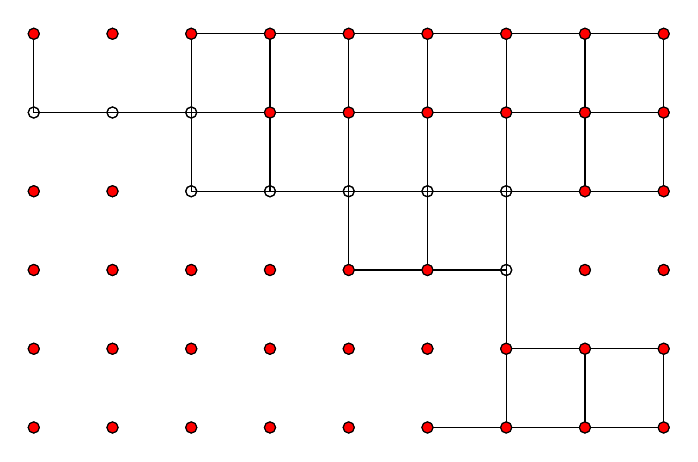
\begin{tikzpicture}[scale=1]%
\path[draw] (0.0,-8.0) -- (1.0,-8.0);%
\path[draw,radius=2pt] (0.0,-8.0) circle;%
\path[draw] (1.0,-8.0) -- (0.0,-8.0);%
\path[draw] (1.0,-8.0) -- (2.0,-8.0);%
\path[draw,radius=2pt] (1.0,-8.0) circle;%
\path[draw] (2.0,-8.0) -- (2.0,-9.0);%
\path[draw] (2.0,-8.0) -- (1.0,-8.0);%
\path[draw,radius=2pt] (2.0,-8.0) circle;%
\path[draw] (2.0,-9.0) -- (2.0,-8.0);%
\path[draw] (2.0,-9.0) -- (3.0,-9.0);%
\path[draw,radius=2pt] (2.0,-9.0) circle;%
\path[draw] (3.0,-9.0) -- (2.0,-9.0);%
\path[draw] (3.0,-9.0) -- (4.0,-9.0);%
\path[draw,radius=2pt] (3.0,-9.0) circle;%
\path[draw] (4.0,-9.0) -- (3.0,-9.0);%
\path[draw] (4.0,-9.0) -- (5.0,-9.0);%
\path[draw,radius=2pt] (4.0,-9.0) circle;%
\path[draw] (5.0,-9.0) -- (4.0,-9.0);%
\path[draw] (5.0,-9.0) -- (6.0,-9.0);%
\path[draw,radius=2pt] (5.0,-9.0) circle;%
\path[draw] (6.0,-9.0) -- (6.0,-10.0);%
\path[draw] (6.0,-9.0) -- (5.0,-9.0);%
\path[draw,radius=2pt] (6.0,-9.0) circle;%
\path[draw] (6.0,-10.0) -- (6.0,-9.0);%
\path[draw] (6.0,-10.0) -- (6.0,-11.0);%
\path[draw,radius=2pt] (6.0,-10.0) circle;%
\path[draw] (6.0,-11.0) -- (6.0,-10.0);%
\path[draw] (6.0,-11.0) -- (6.0,-12.0);%
\path[draw] (6.0,-11.0) -- (7.0,-11.0);%
\path[draw,radius=2pt] (6.0,-11.0) circle;%
\path[draw] (7.0,-11.0) -- (7.0,-12.0);%
\path[draw] (7.0,-11.0) -- (6.0,-11.0);%
\path[draw] (7.0,-11.0) -- (8.0,-11.0);%
\path[draw,radius=2pt] (7.0,-11.0) circle;%
\path[draw] (8.0,-11.0) -- (8.0,-12.0);%
\path[draw] (8.0,-11.0) -- (7.0,-11.0);%
\path[draw,radius=2pt] (8.0,-11.0) circle;%
\path[draw] (5.0,-12.0) -- (6.0,-12.0);%
\path[draw,radius=2pt] (5.0,-12.0) circle;%
\path[draw] (6.0,-12.0) -- (6.0,-11.0);%
\path[draw] (6.0,-12.0) -- (5.0,-12.0);%
\path[draw] (6.0,-12.0) -- (7.0,-12.0);%
\path[draw,radius=2pt] (6.0,-12.0) circle;%
\path[draw] (7.0,-12.0) -- (7.0,-11.0);%
\path[draw] (7.0,-12.0) -- (6.0,-12.0);%
\path[draw] (7.0,-12.0) -- (8.0,-12.0);%
\path[draw,radius=2pt] (7.0,-12.0) circle;%
\path[draw] (8.0,-12.0) -- (8.0,-11.0);%
\path[draw] (8.0,-12.0) -- (7.0,-12.0);%
\path[draw,radius=2pt] (8.0,-12.0) circle;%
\path[draw] (0.0,-7.0) -- (0.0,-8.0);%
\path[draw,radius=2pt] (0.0,-7.0) circle;%
\path[draw] (2.0,-7.0) -- (2.0,-8.0);%
\path[draw] (2.0,-7.0) -- (3.0,-7.0);%
\path[draw,radius=2pt] (2.0,-7.0) circle;%
\path[draw] (3.0,-7.0) -- (3.0,-8.0);%
\path[draw] (3.0,-7.0) -- (2.0,-7.0);%
\path[draw] (3.0,-7.0) -- (4.0,-7.0);%
\path[draw,radius=2pt] (3.0,-7.0) circle;%
\path[draw] (4.0,-7.0) -- (4.0,-8.0);%
\path[draw] (4.0,-7.0) -- (3.0,-7.0);%
\path[draw] (4.0,-7.0) -- (5.0,-7.0);%
\path[draw,radius=2pt] (4.0,-7.0) circle;%
\path[draw] (5.0,-7.0) -- (5.0,-8.0);%
\path[draw] (5.0,-7.0) -- (4.0,-7.0);%
\path[draw] (5.0,-7.0) -- (6.0,-7.0);%
\path[draw,radius=2pt] (5.0,-7.0) circle;%
\path[draw] (6.0,-7.0) -- (6.0,-8.0);%
\path[draw] (6.0,-7.0) -- (5.0,-7.0);%
\path[draw] (6.0,-7.0) -- (7.0,-7.0);%
\path[draw,radius=2pt] (6.0,-7.0) circle;%
\path[draw] (7.0,-7.0) -- (7.0,-8.0);%
\path[draw] (7.0,-7.0) -- (6.0,-7.0);%
\path[draw] (7.0,-7.0) -- (8.0,-7.0);%
\path[draw,radius=2pt] (7.0,-7.0) circle;%
\path[draw] (8.0,-7.0) -- (8.0,-8.0);%
\path[draw] (8.0,-7.0) -- (7.0,-7.0);%
\path[draw,radius=2pt] (8.0,-7.0) circle;%
\path[draw] (0.0,-8.0) -- (0.0,-7.0);%
\path[draw] (0.0,-8.0) -- (1.0,-8.0);%
\path[draw,radius=2pt] (0.0,-8.0) circle;%
\path[draw] (1.0,-8.0) -- (0.0,-8.0);%
\path[draw] (1.0,-8.0) -- (2.0,-8.0);%
\path[draw,radius=2pt] (1.0,-8.0) circle;%
\path[draw] (2.0,-8.0) -- (2.0,-7.0);%
\path[draw] (2.0,-8.0) -- (2.0,-9.0);%
\path[draw] (2.0,-8.0) -- (1.0,-8.0);%
\path[draw] (2.0,-8.0) -- (3.0,-8.0);%
\path[draw,radius=2pt] (2.0,-8.0) circle;%
\path[draw] (3.0,-8.0) -- (3.0,-7.0);%
\path[draw] (3.0,-8.0) -- (3.0,-9.0);%
\path[draw] (3.0,-8.0) -- (2.0,-8.0);%
\path[draw] (3.0,-8.0) -- (4.0,-8.0);%
\path[draw,radius=2pt] (3.0,-8.0) circle;%
\path[draw] (4.0,-8.0) -- (4.0,-7.0);%
\path[draw] (4.0,-8.0) -- (4.0,-9.0);%
\path[draw] (4.0,-8.0) -- (3.0,-8.0);%
\path[draw] (4.0,-8.0) -- (5.0,-8.0);%
\path[draw,radius=2pt] (4.0,-8.0) circle;%
\path[draw] (5.0,-8.0) -- (5.0,-7.0);%
\path[draw] (5.0,-8.0) -- (5.0,-9.0);%
\path[draw] (5.0,-8.0) -- (4.0,-8.0);%
\path[draw] (5.0,-8.0) -- (6.0,-8.0);%
\path[draw,radius=2pt] (5.0,-8.0) circle;%
\path[draw] (6.0,-8.0) -- (6.0,-7.0);%
\path[draw] (6.0,-8.0) -- (6.0,-9.0);%
\path[draw] (6.0,-8.0) -- (5.0,-8.0);%
\path[draw] (6.0,-8.0) -- (7.0,-8.0);%
\path[draw,radius=2pt] (6.0,-8.0) circle;%
\path[draw] (7.0,-8.0) -- (7.0,-7.0);%
\path[draw] (7.0,-8.0) -- (7.0,-9.0);%
\path[draw] (7.0,-8.0) -- (6.0,-8.0);%
\path[draw] (7.0,-8.0) -- (8.0,-8.0);%
\path[draw,radius=2pt] (7.0,-8.0) circle;%
\path[draw] (8.0,-8.0) -- (8.0,-7.0);%
\path[draw] (8.0,-8.0) -- (8.0,-9.0);%
\path[draw] (8.0,-8.0) -- (7.0,-8.0);%
\path[draw,radius=2pt] (8.0,-8.0) circle;%
\path[draw] (2.0,-9.0) -- (2.0,-8.0);%
\path[draw] (2.0,-9.0) -- (3.0,-9.0);%
\path[draw,radius=2pt] (2.0,-9.0) circle;%
\path[draw] (3.0,-9.0) -- (3.0,-8.0);%
\path[draw] (3.0,-9.0) -- (2.0,-9.0);%
\path[draw] (3.0,-9.0) -- (4.0,-9.0);%
\path[draw,radius=2pt] (3.0,-9.0) circle;%
\path[draw] (4.0,-9.0) -- (4.0,-8.0);%
\path[draw] (4.0,-9.0) -- (4.0,-10.0);%
\path[draw] (4.0,-9.0) -- (3.0,-9.0);%
\path[draw] (4.0,-9.0) -- (5.0,-9.0);%
\path[draw,radius=2pt] (4.0,-9.0) circle;%
\path[draw] (5.0,-9.0) -- (5.0,-8.0);%
\path[draw] (5.0,-9.0) -- (5.0,-10.0);%
\path[draw] (5.0,-9.0) -- (4.0,-9.0);%
\path[draw] (5.0,-9.0) -- (6.0,-9.0);%
\path[draw,radius=2pt] (5.0,-9.0) circle;%
\path[draw] (6.0,-9.0) -- (6.0,-8.0);%
\path[draw] (6.0,-9.0) -- (6.0,-10.0);%
\path[draw] (6.0,-9.0) -- (5.0,-9.0);%
\path[draw] (6.0,-9.0) -- (7.0,-9.0);%
\path[draw,radius=2pt] (6.0,-9.0) circle;%
\path[draw] (7.0,-9.0) -- (7.0,-8.0);%
\path[draw] (7.0,-9.0) -- (6.0,-9.0);%
\path[draw] (7.0,-9.0) -- (8.0,-9.0);%
\path[draw,radius=2pt] (7.0,-9.0) circle;%
\path[draw] (8.0,-9.0) -- (8.0,-8.0);%
\path[draw] (8.0,-9.0) -- (7.0,-9.0);%
\path[draw,radius=2pt] (8.0,-9.0) circle;%
\path[draw] (4.0,-10.0) -- (4.0,-9.0);%
\path[draw] (4.0,-10.0) -- (5.0,-10.0);%
\path[draw,radius=2pt] (4.0,-10.0) circle;%
\path[draw] (5.0,-10.0) -- (5.0,-9.0);%
\path[draw] (5.0,-10.0) -- (4.0,-10.0);%
\path[draw] (5.0,-10.0) -- (6.0,-10.0);%
\path[draw,radius=2pt] (5.0,-10.0) circle;%
\path[draw] (6.0,-10.0) -- (6.0,-9.0);%
\path[draw] (6.0,-10.0) -- (5.0,-10.0);%
\path[draw,radius=2pt] (6.0,-10.0) circle;%
\path[draw,radius=2pt,fill=red] (0.0,-7.0) circle;%
\path[draw,radius=2pt,fill=red] (1.0,-7.0) circle;%
\path[draw,radius=2pt,fill=red] (2.0,-7.0) circle;%
\path[draw,radius=2pt,fill=red] (3.0,-7.0) circle;%
\path[draw,radius=2pt,fill=red] (4.0,-7.0) circle;%
\path[draw,radius=2pt,fill=red] (5.0,-7.0) circle;%
\path[draw,radius=2pt,fill=red] (6.0,-7.0) circle;%
\path[draw,radius=2pt,fill=red] (7.0,-7.0) circle;%
\path[draw,radius=2pt,fill=red] (8.0,-7.0) circle;%
\path[draw,radius=2pt,fill=red] (3.0,-8.0) circle;%
\path[draw,radius=2pt,fill=red] (4.0,-8.0) circle;%
\path[draw,radius=2pt,fill=red] (5.0,-8.0) circle;%
\path[draw,radius=2pt,fill=red] (6.0,-8.0) circle;%
\path[draw,radius=2pt,fill=red] (7.0,-8.0) circle;%
\path[draw,radius=2pt,fill=red] (8.0,-8.0) circle;%
\path[draw,radius=2pt,fill=red] (0.0,-9.0) circle;%
\path[draw,radius=2pt,fill=red] (1.0,-9.0) circle;%
\path[draw,radius=2pt,fill=red] (7.0,-9.0) circle;%
\path[draw,radius=2pt,fill=red] (8.0,-9.0) circle;%
\path[draw,radius=2pt,fill=red] (0.0,-10.0) circle;%
\path[draw,radius=2pt,fill=red] (1.0,-10.0) circle;%
\path[draw,radius=2pt,fill=red] (2.0,-10.0) circle;%
\path[draw,radius=2pt,fill=red] (3.0,-10.0) circle;%
\path[draw,radius=2pt,fill=red] (4.0,-10.0) circle;%
\path[draw,radius=2pt,fill=red] (5.0,-10.0) circle;%
\path[draw,radius=2pt,fill=red] (7.0,-10.0) circle;%
\path[draw,radius=2pt,fill=red] (8.0,-10.0) circle;%
\path[draw,radius=2pt,fill=red] (0.0,-11.0) circle;%
\path[draw,radius=2pt,fill=red] (1.0,-11.0) circle;%
\path[draw,radius=2pt,fill=red] (2.0,-11.0) circle;%
\path[draw,radius=2pt,fill=red] (3.0,-11.0) circle;%
\path[draw,radius=2pt,fill=red] (4.0,-11.0) circle;%
\path[draw,radius=2pt,fill=red] (5.0,-11.0) circle;%
\path[draw,radius=2pt,fill=red] (0.0,-12.0) circle;%
\path[draw,radius=2pt,fill=red] (1.0,-12.0) circle;%
\path[draw,radius=2pt,fill=red] (2.0,-12.0) circle;%
\path[draw,radius=2pt,fill=red] (3.0,-12.0) circle;%
\path[draw,radius=2pt,fill=red] (4.0,-12.0) circle;%
\path[draw,radius=2pt,fill=red] (1.0,-7.0) circle;%
\path[draw,radius=2pt,fill=red] (0.0,-9.0) circle;%
\path[draw,radius=2pt,fill=red] (1.0,-9.0) circle;%
\path[draw,radius=2pt,fill=red] (0.0,-10.0) circle;%
\path[draw,radius=2pt,fill=red] (1.0,-10.0) circle;%
\path[draw,radius=2pt,fill=red] (2.0,-10.0) circle;%
\path[draw,radius=2pt,fill=red] (3.0,-10.0) circle;%
\path[draw,radius=2pt,fill=red] (7.0,-10.0) circle;%
\path[draw,radius=2pt,fill=red] (8.0,-10.0) circle;%
\path[draw,radius=2pt,fill=red] (0.0,-11.0) circle;%
\path[draw,radius=2pt,fill=red] (1.0,-11.0) circle;%
\path[draw,radius=2pt,fill=red] (2.0,-11.0) circle;%
\path[draw,radius=2pt,fill=red] (3.0,-11.0) circle;%
\path[draw,radius=2pt,fill=red] (4.0,-11.0) circle;%
\path[draw,radius=2pt,fill=red] (5.0,-11.0) circle;%
\path[draw,radius=2pt,fill=red] (6.0,-11.0) circle;%
\path[draw,radius=2pt,fill=red] (7.0,-11.0) circle;%
\path[draw,radius=2pt,fill=red] (8.0,-11.0) circle;%
\path[draw,radius=2pt,fill=red] (0.0,-12.0) circle;%
\path[draw,radius=2pt,fill=red] (1.0,-12.0) circle;%
\path[draw,radius=2pt,fill=red] (2.0,-12.0) circle;%
\path[draw,radius=2pt,fill=red] (3.0,-12.0) circle;%
\path[draw,radius=2pt,fill=red] (4.0,-12.0) circle;%
\path[draw,radius=2pt,fill=red] (5.0,-12.0) circle;%
\path[draw,radius=2pt,fill=red] (6.0,-12.0) circle;%
\path[draw,radius=2pt,fill=red] (7.0,-12.0) circle;%
\path[draw,radius=2pt,fill=red] (8.0,-12.0) circle;%
\end{tikzpicture}%
\newline%
\hspace*{1in}%
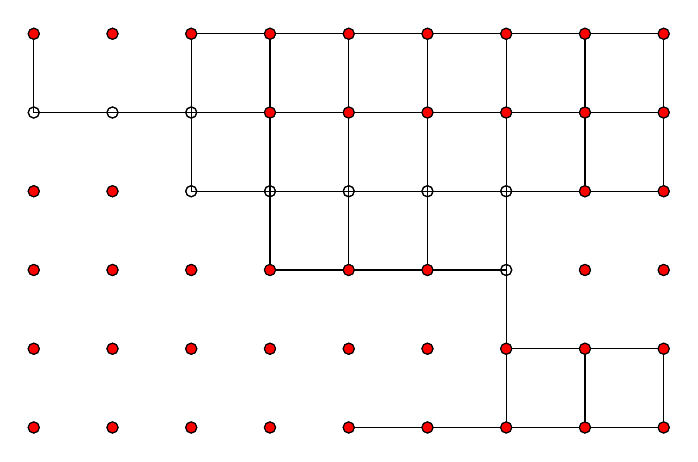
\begin{tikzpicture}[scale=1]%
\path[draw] (0.0,-8.0) -- (1.0,-8.0);%
\path[draw,radius=2pt] (0.0,-8.0) circle;%
\path[draw] (1.0,-8.0) -- (0.0,-8.0);%
\path[draw] (1.0,-8.0) -- (2.0,-8.0);%
\path[draw,radius=2pt] (1.0,-8.0) circle;%
\path[draw] (2.0,-8.0) -- (2.0,-9.0);%
\path[draw] (2.0,-8.0) -- (1.0,-8.0);%
\path[draw,radius=2pt] (2.0,-8.0) circle;%
\path[draw] (2.0,-9.0) -- (2.0,-8.0);%
\path[draw] (2.0,-9.0) -- (3.0,-9.0);%
\path[draw,radius=2pt] (2.0,-9.0) circle;%
\path[draw] (3.0,-9.0) -- (2.0,-9.0);%
\path[draw] (3.0,-9.0) -- (4.0,-9.0);%
\path[draw,radius=2pt] (3.0,-9.0) circle;%
\path[draw] (4.0,-9.0) -- (3.0,-9.0);%
\path[draw] (4.0,-9.0) -- (5.0,-9.0);%
\path[draw,radius=2pt] (4.0,-9.0) circle;%
\path[draw] (5.0,-9.0) -- (4.0,-9.0);%
\path[draw] (5.0,-9.0) -- (6.0,-9.0);%
\path[draw,radius=2pt] (5.0,-9.0) circle;%
\path[draw] (6.0,-9.0) -- (6.0,-10.0);%
\path[draw] (6.0,-9.0) -- (5.0,-9.0);%
\path[draw,radius=2pt] (6.0,-9.0) circle;%
\path[draw] (6.0,-10.0) -- (6.0,-9.0);%
\path[draw] (6.0,-10.0) -- (6.0,-11.0);%
\path[draw,radius=2pt] (6.0,-10.0) circle;%
\path[draw] (6.0,-11.0) -- (6.0,-10.0);%
\path[draw] (6.0,-11.0) -- (6.0,-12.0);%
\path[draw] (6.0,-11.0) -- (7.0,-11.0);%
\path[draw,radius=2pt] (6.0,-11.0) circle;%
\path[draw] (7.0,-11.0) -- (7.0,-12.0);%
\path[draw] (7.0,-11.0) -- (6.0,-11.0);%
\path[draw] (7.0,-11.0) -- (8.0,-11.0);%
\path[draw,radius=2pt] (7.0,-11.0) circle;%
\path[draw] (8.0,-11.0) -- (8.0,-12.0);%
\path[draw] (8.0,-11.0) -- (7.0,-11.0);%
\path[draw,radius=2pt] (8.0,-11.0) circle;%
\path[draw] (4.0,-12.0) -- (5.0,-12.0);%
\path[draw,radius=2pt] (4.0,-12.0) circle;%
\path[draw] (5.0,-12.0) -- (4.0,-12.0);%
\path[draw] (5.0,-12.0) -- (6.0,-12.0);%
\path[draw,radius=2pt] (5.0,-12.0) circle;%
\path[draw] (6.0,-12.0) -- (6.0,-11.0);%
\path[draw] (6.0,-12.0) -- (5.0,-12.0);%
\path[draw] (6.0,-12.0) -- (7.0,-12.0);%
\path[draw,radius=2pt] (6.0,-12.0) circle;%
\path[draw] (7.0,-12.0) -- (7.0,-11.0);%
\path[draw] (7.0,-12.0) -- (6.0,-12.0);%
\path[draw] (7.0,-12.0) -- (8.0,-12.0);%
\path[draw,radius=2pt] (7.0,-12.0) circle;%
\path[draw] (8.0,-12.0) -- (8.0,-11.0);%
\path[draw] (8.0,-12.0) -- (7.0,-12.0);%
\path[draw,radius=2pt] (8.0,-12.0) circle;%
\path[draw] (0.0,-7.0) -- (0.0,-8.0);%
\path[draw,radius=2pt] (0.0,-7.0) circle;%
\path[draw] (2.0,-7.0) -- (2.0,-8.0);%
\path[draw] (2.0,-7.0) -- (3.0,-7.0);%
\path[draw,radius=2pt] (2.0,-7.0) circle;%
\path[draw] (3.0,-7.0) -- (3.0,-8.0);%
\path[draw] (3.0,-7.0) -- (2.0,-7.0);%
\path[draw] (3.0,-7.0) -- (4.0,-7.0);%
\path[draw,radius=2pt] (3.0,-7.0) circle;%
\path[draw] (4.0,-7.0) -- (4.0,-8.0);%
\path[draw] (4.0,-7.0) -- (3.0,-7.0);%
\path[draw] (4.0,-7.0) -- (5.0,-7.0);%
\path[draw,radius=2pt] (4.0,-7.0) circle;%
\path[draw] (5.0,-7.0) -- (5.0,-8.0);%
\path[draw] (5.0,-7.0) -- (4.0,-7.0);%
\path[draw] (5.0,-7.0) -- (6.0,-7.0);%
\path[draw,radius=2pt] (5.0,-7.0) circle;%
\path[draw] (6.0,-7.0) -- (6.0,-8.0);%
\path[draw] (6.0,-7.0) -- (5.0,-7.0);%
\path[draw] (6.0,-7.0) -- (7.0,-7.0);%
\path[draw,radius=2pt] (6.0,-7.0) circle;%
\path[draw] (7.0,-7.0) -- (7.0,-8.0);%
\path[draw] (7.0,-7.0) -- (6.0,-7.0);%
\path[draw] (7.0,-7.0) -- (8.0,-7.0);%
\path[draw,radius=2pt] (7.0,-7.0) circle;%
\path[draw] (8.0,-7.0) -- (8.0,-8.0);%
\path[draw] (8.0,-7.0) -- (7.0,-7.0);%
\path[draw,radius=2pt] (8.0,-7.0) circle;%
\path[draw] (0.0,-8.0) -- (0.0,-7.0);%
\path[draw] (0.0,-8.0) -- (1.0,-8.0);%
\path[draw,radius=2pt] (0.0,-8.0) circle;%
\path[draw] (1.0,-8.0) -- (0.0,-8.0);%
\path[draw] (1.0,-8.0) -- (2.0,-8.0);%
\path[draw,radius=2pt] (1.0,-8.0) circle;%
\path[draw] (2.0,-8.0) -- (2.0,-7.0);%
\path[draw] (2.0,-8.0) -- (2.0,-9.0);%
\path[draw] (2.0,-8.0) -- (1.0,-8.0);%
\path[draw] (2.0,-8.0) -- (3.0,-8.0);%
\path[draw,radius=2pt] (2.0,-8.0) circle;%
\path[draw] (3.0,-8.0) -- (3.0,-7.0);%
\path[draw] (3.0,-8.0) -- (3.0,-9.0);%
\path[draw] (3.0,-8.0) -- (2.0,-8.0);%
\path[draw] (3.0,-8.0) -- (4.0,-8.0);%
\path[draw,radius=2pt] (3.0,-8.0) circle;%
\path[draw] (4.0,-8.0) -- (4.0,-7.0);%
\path[draw] (4.0,-8.0) -- (4.0,-9.0);%
\path[draw] (4.0,-8.0) -- (3.0,-8.0);%
\path[draw] (4.0,-8.0) -- (5.0,-8.0);%
\path[draw,radius=2pt] (4.0,-8.0) circle;%
\path[draw] (5.0,-8.0) -- (5.0,-7.0);%
\path[draw] (5.0,-8.0) -- (5.0,-9.0);%
\path[draw] (5.0,-8.0) -- (4.0,-8.0);%
\path[draw] (5.0,-8.0) -- (6.0,-8.0);%
\path[draw,radius=2pt] (5.0,-8.0) circle;%
\path[draw] (6.0,-8.0) -- (6.0,-7.0);%
\path[draw] (6.0,-8.0) -- (6.0,-9.0);%
\path[draw] (6.0,-8.0) -- (5.0,-8.0);%
\path[draw] (6.0,-8.0) -- (7.0,-8.0);%
\path[draw,radius=2pt] (6.0,-8.0) circle;%
\path[draw] (7.0,-8.0) -- (7.0,-7.0);%
\path[draw] (7.0,-8.0) -- (7.0,-9.0);%
\path[draw] (7.0,-8.0) -- (6.0,-8.0);%
\path[draw] (7.0,-8.0) -- (8.0,-8.0);%
\path[draw,radius=2pt] (7.0,-8.0) circle;%
\path[draw] (8.0,-8.0) -- (8.0,-7.0);%
\path[draw] (8.0,-8.0) -- (8.0,-9.0);%
\path[draw] (8.0,-8.0) -- (7.0,-8.0);%
\path[draw,radius=2pt] (8.0,-8.0) circle;%
\path[draw] (2.0,-9.0) -- (2.0,-8.0);%
\path[draw] (2.0,-9.0) -- (3.0,-9.0);%
\path[draw,radius=2pt] (2.0,-9.0) circle;%
\path[draw] (3.0,-9.0) -- (3.0,-8.0);%
\path[draw] (3.0,-9.0) -- (3.0,-10.0);%
\path[draw] (3.0,-9.0) -- (2.0,-9.0);%
\path[draw] (3.0,-9.0) -- (4.0,-9.0);%
\path[draw,radius=2pt] (3.0,-9.0) circle;%
\path[draw] (4.0,-9.0) -- (4.0,-8.0);%
\path[draw] (4.0,-9.0) -- (4.0,-10.0);%
\path[draw] (4.0,-9.0) -- (3.0,-9.0);%
\path[draw] (4.0,-9.0) -- (5.0,-9.0);%
\path[draw,radius=2pt] (4.0,-9.0) circle;%
\path[draw] (5.0,-9.0) -- (5.0,-8.0);%
\path[draw] (5.0,-9.0) -- (5.0,-10.0);%
\path[draw] (5.0,-9.0) -- (4.0,-9.0);%
\path[draw] (5.0,-9.0) -- (6.0,-9.0);%
\path[draw,radius=2pt] (5.0,-9.0) circle;%
\path[draw] (6.0,-9.0) -- (6.0,-8.0);%
\path[draw] (6.0,-9.0) -- (6.0,-10.0);%
\path[draw] (6.0,-9.0) -- (5.0,-9.0);%
\path[draw] (6.0,-9.0) -- (7.0,-9.0);%
\path[draw,radius=2pt] (6.0,-9.0) circle;%
\path[draw] (7.0,-9.0) -- (7.0,-8.0);%
\path[draw] (7.0,-9.0) -- (6.0,-9.0);%
\path[draw] (7.0,-9.0) -- (8.0,-9.0);%
\path[draw,radius=2pt] (7.0,-9.0) circle;%
\path[draw] (8.0,-9.0) -- (8.0,-8.0);%
\path[draw] (8.0,-9.0) -- (7.0,-9.0);%
\path[draw,radius=2pt] (8.0,-9.0) circle;%
\path[draw] (3.0,-10.0) -- (3.0,-9.0);%
\path[draw] (3.0,-10.0) -- (4.0,-10.0);%
\path[draw,radius=2pt] (3.0,-10.0) circle;%
\path[draw] (4.0,-10.0) -- (4.0,-9.0);%
\path[draw] (4.0,-10.0) -- (3.0,-10.0);%
\path[draw] (4.0,-10.0) -- (5.0,-10.0);%
\path[draw,radius=2pt] (4.0,-10.0) circle;%
\path[draw] (5.0,-10.0) -- (5.0,-9.0);%
\path[draw] (5.0,-10.0) -- (4.0,-10.0);%
\path[draw] (5.0,-10.0) -- (6.0,-10.0);%
\path[draw,radius=2pt] (5.0,-10.0) circle;%
\path[draw] (6.0,-10.0) -- (6.0,-9.0);%
\path[draw] (6.0,-10.0) -- (5.0,-10.0);%
\path[draw,radius=2pt] (6.0,-10.0) circle;%
\path[draw,radius=2pt,fill=red] (0.0,-7.0) circle;%
\path[draw,radius=2pt,fill=red] (1.0,-7.0) circle;%
\path[draw,radius=2pt,fill=red] (2.0,-7.0) circle;%
\path[draw,radius=2pt,fill=red] (3.0,-7.0) circle;%
\path[draw,radius=2pt,fill=red] (4.0,-7.0) circle;%
\path[draw,radius=2pt,fill=red] (5.0,-7.0) circle;%
\path[draw,radius=2pt,fill=red] (6.0,-7.0) circle;%
\path[draw,radius=2pt,fill=red] (7.0,-7.0) circle;%
\path[draw,radius=2pt,fill=red] (8.0,-7.0) circle;%
\path[draw,radius=2pt,fill=red] (3.0,-8.0) circle;%
\path[draw,radius=2pt,fill=red] (4.0,-8.0) circle;%
\path[draw,radius=2pt,fill=red] (5.0,-8.0) circle;%
\path[draw,radius=2pt,fill=red] (6.0,-8.0) circle;%
\path[draw,radius=2pt,fill=red] (7.0,-8.0) circle;%
\path[draw,radius=2pt,fill=red] (8.0,-8.0) circle;%
\path[draw,radius=2pt,fill=red] (0.0,-9.0) circle;%
\path[draw,radius=2pt,fill=red] (1.0,-9.0) circle;%
\path[draw,radius=2pt,fill=red] (7.0,-9.0) circle;%
\path[draw,radius=2pt,fill=red] (8.0,-9.0) circle;%
\path[draw,radius=2pt,fill=red] (0.0,-10.0) circle;%
\path[draw,radius=2pt,fill=red] (1.0,-10.0) circle;%
\path[draw,radius=2pt,fill=red] (2.0,-10.0) circle;%
\path[draw,radius=2pt,fill=red] (3.0,-10.0) circle;%
\path[draw,radius=2pt,fill=red] (4.0,-10.0) circle;%
\path[draw,radius=2pt,fill=red] (5.0,-10.0) circle;%
\path[draw,radius=2pt,fill=red] (7.0,-10.0) circle;%
\path[draw,radius=2pt,fill=red] (8.0,-10.0) circle;%
\path[draw,radius=2pt,fill=red] (0.0,-11.0) circle;%
\path[draw,radius=2pt,fill=red] (1.0,-11.0) circle;%
\path[draw,radius=2pt,fill=red] (2.0,-11.0) circle;%
\path[draw,radius=2pt,fill=red] (3.0,-11.0) circle;%
\path[draw,radius=2pt,fill=red] (4.0,-11.0) circle;%
\path[draw,radius=2pt,fill=red] (5.0,-11.0) circle;%
\path[draw,radius=2pt,fill=red] (0.0,-12.0) circle;%
\path[draw,radius=2pt,fill=red] (1.0,-12.0) circle;%
\path[draw,radius=2pt,fill=red] (2.0,-12.0) circle;%
\path[draw,radius=2pt,fill=red] (3.0,-12.0) circle;%
\path[draw,radius=2pt,fill=red] (1.0,-7.0) circle;%
\path[draw,radius=2pt,fill=red] (0.0,-9.0) circle;%
\path[draw,radius=2pt,fill=red] (1.0,-9.0) circle;%
\path[draw,radius=2pt,fill=red] (0.0,-10.0) circle;%
\path[draw,radius=2pt,fill=red] (1.0,-10.0) circle;%
\path[draw,radius=2pt,fill=red] (2.0,-10.0) circle;%
\path[draw,radius=2pt,fill=red] (7.0,-10.0) circle;%
\path[draw,radius=2pt,fill=red] (8.0,-10.0) circle;%
\path[draw,radius=2pt,fill=red] (0.0,-11.0) circle;%
\path[draw,radius=2pt,fill=red] (1.0,-11.0) circle;%
\path[draw,radius=2pt,fill=red] (2.0,-11.0) circle;%
\path[draw,radius=2pt,fill=red] (3.0,-11.0) circle;%
\path[draw,radius=2pt,fill=red] (4.0,-11.0) circle;%
\path[draw,radius=2pt,fill=red] (5.0,-11.0) circle;%
\path[draw,radius=2pt,fill=red] (6.0,-11.0) circle;%
\path[draw,radius=2pt,fill=red] (7.0,-11.0) circle;%
\path[draw,radius=2pt,fill=red] (8.0,-11.0) circle;%
\path[draw,radius=2pt,fill=red] (0.0,-12.0) circle;%
\path[draw,radius=2pt,fill=red] (1.0,-12.0) circle;%
\path[draw,radius=2pt,fill=red] (2.0,-12.0) circle;%
\path[draw,radius=2pt,fill=red] (3.0,-12.0) circle;%
\path[draw,radius=2pt,fill=red] (4.0,-12.0) circle;%
\path[draw,radius=2pt,fill=red] (5.0,-12.0) circle;%
\path[draw,radius=2pt,fill=red] (6.0,-12.0) circle;%
\path[draw,radius=2pt,fill=red] (7.0,-12.0) circle;%
\path[draw,radius=2pt,fill=red] (8.0,-12.0) circle;%
\end{tikzpicture}%
\hspace*{1in}%
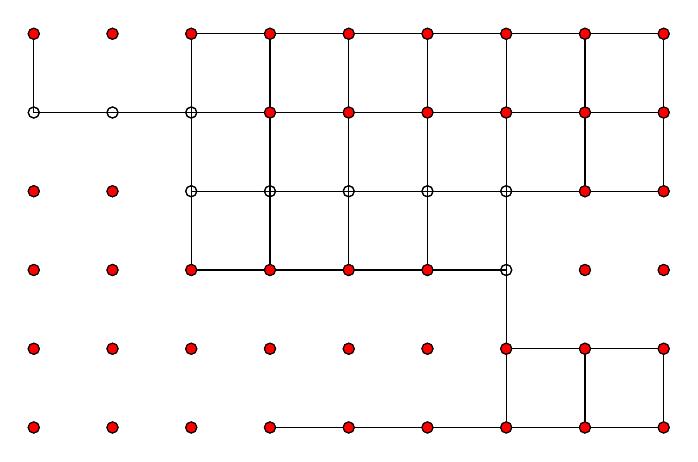
\begin{tikzpicture}[scale=1]%
\path[draw] (0.0,-8.0) -- (1.0,-8.0);%
\path[draw,radius=2pt] (0.0,-8.0) circle;%
\path[draw] (1.0,-8.0) -- (0.0,-8.0);%
\path[draw] (1.0,-8.0) -- (2.0,-8.0);%
\path[draw,radius=2pt] (1.0,-8.0) circle;%
\path[draw] (2.0,-8.0) -- (2.0,-9.0);%
\path[draw] (2.0,-8.0) -- (1.0,-8.0);%
\path[draw,radius=2pt] (2.0,-8.0) circle;%
\path[draw] (2.0,-9.0) -- (2.0,-8.0);%
\path[draw] (2.0,-9.0) -- (3.0,-9.0);%
\path[draw,radius=2pt] (2.0,-9.0) circle;%
\path[draw] (3.0,-9.0) -- (2.0,-9.0);%
\path[draw] (3.0,-9.0) -- (4.0,-9.0);%
\path[draw,radius=2pt] (3.0,-9.0) circle;%
\path[draw] (4.0,-9.0) -- (3.0,-9.0);%
\path[draw] (4.0,-9.0) -- (5.0,-9.0);%
\path[draw,radius=2pt] (4.0,-9.0) circle;%
\path[draw] (5.0,-9.0) -- (4.0,-9.0);%
\path[draw] (5.0,-9.0) -- (6.0,-9.0);%
\path[draw,radius=2pt] (5.0,-9.0) circle;%
\path[draw] (6.0,-9.0) -- (6.0,-10.0);%
\path[draw] (6.0,-9.0) -- (5.0,-9.0);%
\path[draw,radius=2pt] (6.0,-9.0) circle;%
\path[draw] (6.0,-10.0) -- (6.0,-9.0);%
\path[draw] (6.0,-10.0) -- (6.0,-11.0);%
\path[draw,radius=2pt] (6.0,-10.0) circle;%
\path[draw] (6.0,-11.0) -- (6.0,-10.0);%
\path[draw] (6.0,-11.0) -- (6.0,-12.0);%
\path[draw] (6.0,-11.0) -- (7.0,-11.0);%
\path[draw,radius=2pt] (6.0,-11.0) circle;%
\path[draw] (7.0,-11.0) -- (7.0,-12.0);%
\path[draw] (7.0,-11.0) -- (6.0,-11.0);%
\path[draw] (7.0,-11.0) -- (8.0,-11.0);%
\path[draw,radius=2pt] (7.0,-11.0) circle;%
\path[draw] (8.0,-11.0) -- (8.0,-12.0);%
\path[draw] (8.0,-11.0) -- (7.0,-11.0);%
\path[draw,radius=2pt] (8.0,-11.0) circle;%
\path[draw] (3.0,-12.0) -- (4.0,-12.0);%
\path[draw,radius=2pt] (3.0,-12.0) circle;%
\path[draw] (4.0,-12.0) -- (3.0,-12.0);%
\path[draw] (4.0,-12.0) -- (5.0,-12.0);%
\path[draw,radius=2pt] (4.0,-12.0) circle;%
\path[draw] (5.0,-12.0) -- (4.0,-12.0);%
\path[draw] (5.0,-12.0) -- (6.0,-12.0);%
\path[draw,radius=2pt] (5.0,-12.0) circle;%
\path[draw] (6.0,-12.0) -- (6.0,-11.0);%
\path[draw] (6.0,-12.0) -- (5.0,-12.0);%
\path[draw] (6.0,-12.0) -- (7.0,-12.0);%
\path[draw,radius=2pt] (6.0,-12.0) circle;%
\path[draw] (7.0,-12.0) -- (7.0,-11.0);%
\path[draw] (7.0,-12.0) -- (6.0,-12.0);%
\path[draw] (7.0,-12.0) -- (8.0,-12.0);%
\path[draw,radius=2pt] (7.0,-12.0) circle;%
\path[draw] (8.0,-12.0) -- (8.0,-11.0);%
\path[draw] (8.0,-12.0) -- (7.0,-12.0);%
\path[draw,radius=2pt] (8.0,-12.0) circle;%
\path[draw] (0.0,-7.0) -- (0.0,-8.0);%
\path[draw,radius=2pt] (0.0,-7.0) circle;%
\path[draw] (2.0,-7.0) -- (2.0,-8.0);%
\path[draw] (2.0,-7.0) -- (3.0,-7.0);%
\path[draw,radius=2pt] (2.0,-7.0) circle;%
\path[draw] (3.0,-7.0) -- (3.0,-8.0);%
\path[draw] (3.0,-7.0) -- (2.0,-7.0);%
\path[draw] (3.0,-7.0) -- (4.0,-7.0);%
\path[draw,radius=2pt] (3.0,-7.0) circle;%
\path[draw] (4.0,-7.0) -- (4.0,-8.0);%
\path[draw] (4.0,-7.0) -- (3.0,-7.0);%
\path[draw] (4.0,-7.0) -- (5.0,-7.0);%
\path[draw,radius=2pt] (4.0,-7.0) circle;%
\path[draw] (5.0,-7.0) -- (5.0,-8.0);%
\path[draw] (5.0,-7.0) -- (4.0,-7.0);%
\path[draw] (5.0,-7.0) -- (6.0,-7.0);%
\path[draw,radius=2pt] (5.0,-7.0) circle;%
\path[draw] (6.0,-7.0) -- (6.0,-8.0);%
\path[draw] (6.0,-7.0) -- (5.0,-7.0);%
\path[draw] (6.0,-7.0) -- (7.0,-7.0);%
\path[draw,radius=2pt] (6.0,-7.0) circle;%
\path[draw] (7.0,-7.0) -- (7.0,-8.0);%
\path[draw] (7.0,-7.0) -- (6.0,-7.0);%
\path[draw] (7.0,-7.0) -- (8.0,-7.0);%
\path[draw,radius=2pt] (7.0,-7.0) circle;%
\path[draw] (8.0,-7.0) -- (8.0,-8.0);%
\path[draw] (8.0,-7.0) -- (7.0,-7.0);%
\path[draw,radius=2pt] (8.0,-7.0) circle;%
\path[draw] (0.0,-8.0) -- (0.0,-7.0);%
\path[draw] (0.0,-8.0) -- (1.0,-8.0);%
\path[draw,radius=2pt] (0.0,-8.0) circle;%
\path[draw] (1.0,-8.0) -- (0.0,-8.0);%
\path[draw] (1.0,-8.0) -- (2.0,-8.0);%
\path[draw,radius=2pt] (1.0,-8.0) circle;%
\path[draw] (2.0,-8.0) -- (2.0,-7.0);%
\path[draw] (2.0,-8.0) -- (2.0,-9.0);%
\path[draw] (2.0,-8.0) -- (1.0,-8.0);%
\path[draw] (2.0,-8.0) -- (3.0,-8.0);%
\path[draw,radius=2pt] (2.0,-8.0) circle;%
\path[draw] (3.0,-8.0) -- (3.0,-7.0);%
\path[draw] (3.0,-8.0) -- (3.0,-9.0);%
\path[draw] (3.0,-8.0) -- (2.0,-8.0);%
\path[draw] (3.0,-8.0) -- (4.0,-8.0);%
\path[draw,radius=2pt] (3.0,-8.0) circle;%
\path[draw] (4.0,-8.0) -- (4.0,-7.0);%
\path[draw] (4.0,-8.0) -- (4.0,-9.0);%
\path[draw] (4.0,-8.0) -- (3.0,-8.0);%
\path[draw] (4.0,-8.0) -- (5.0,-8.0);%
\path[draw,radius=2pt] (4.0,-8.0) circle;%
\path[draw] (5.0,-8.0) -- (5.0,-7.0);%
\path[draw] (5.0,-8.0) -- (5.0,-9.0);%
\path[draw] (5.0,-8.0) -- (4.0,-8.0);%
\path[draw] (5.0,-8.0) -- (6.0,-8.0);%
\path[draw,radius=2pt] (5.0,-8.0) circle;%
\path[draw] (6.0,-8.0) -- (6.0,-7.0);%
\path[draw] (6.0,-8.0) -- (6.0,-9.0);%
\path[draw] (6.0,-8.0) -- (5.0,-8.0);%
\path[draw] (6.0,-8.0) -- (7.0,-8.0);%
\path[draw,radius=2pt] (6.0,-8.0) circle;%
\path[draw] (7.0,-8.0) -- (7.0,-7.0);%
\path[draw] (7.0,-8.0) -- (7.0,-9.0);%
\path[draw] (7.0,-8.0) -- (6.0,-8.0);%
\path[draw] (7.0,-8.0) -- (8.0,-8.0);%
\path[draw,radius=2pt] (7.0,-8.0) circle;%
\path[draw] (8.0,-8.0) -- (8.0,-7.0);%
\path[draw] (8.0,-8.0) -- (8.0,-9.0);%
\path[draw] (8.0,-8.0) -- (7.0,-8.0);%
\path[draw,radius=2pt] (8.0,-8.0) circle;%
\path[draw] (2.0,-9.0) -- (2.0,-8.0);%
\path[draw] (2.0,-9.0) -- (2.0,-10.0);%
\path[draw] (2.0,-9.0) -- (3.0,-9.0);%
\path[draw,radius=2pt] (2.0,-9.0) circle;%
\path[draw] (3.0,-9.0) -- (3.0,-8.0);%
\path[draw] (3.0,-9.0) -- (3.0,-10.0);%
\path[draw] (3.0,-9.0) -- (2.0,-9.0);%
\path[draw] (3.0,-9.0) -- (4.0,-9.0);%
\path[draw,radius=2pt] (3.0,-9.0) circle;%
\path[draw] (4.0,-9.0) -- (4.0,-8.0);%
\path[draw] (4.0,-9.0) -- (4.0,-10.0);%
\path[draw] (4.0,-9.0) -- (3.0,-9.0);%
\path[draw] (4.0,-9.0) -- (5.0,-9.0);%
\path[draw,radius=2pt] (4.0,-9.0) circle;%
\path[draw] (5.0,-9.0) -- (5.0,-8.0);%
\path[draw] (5.0,-9.0) -- (5.0,-10.0);%
\path[draw] (5.0,-9.0) -- (4.0,-9.0);%
\path[draw] (5.0,-9.0) -- (6.0,-9.0);%
\path[draw,radius=2pt] (5.0,-9.0) circle;%
\path[draw] (6.0,-9.0) -- (6.0,-8.0);%
\path[draw] (6.0,-9.0) -- (6.0,-10.0);%
\path[draw] (6.0,-9.0) -- (5.0,-9.0);%
\path[draw] (6.0,-9.0) -- (7.0,-9.0);%
\path[draw,radius=2pt] (6.0,-9.0) circle;%
\path[draw] (7.0,-9.0) -- (7.0,-8.0);%
\path[draw] (7.0,-9.0) -- (6.0,-9.0);%
\path[draw] (7.0,-9.0) -- (8.0,-9.0);%
\path[draw,radius=2pt] (7.0,-9.0) circle;%
\path[draw] (8.0,-9.0) -- (8.0,-8.0);%
\path[draw] (8.0,-9.0) -- (7.0,-9.0);%
\path[draw,radius=2pt] (8.0,-9.0) circle;%
\path[draw] (2.0,-10.0) -- (2.0,-9.0);%
\path[draw] (2.0,-10.0) -- (3.0,-10.0);%
\path[draw,radius=2pt] (2.0,-10.0) circle;%
\path[draw] (3.0,-10.0) -- (3.0,-9.0);%
\path[draw] (3.0,-10.0) -- (2.0,-10.0);%
\path[draw] (3.0,-10.0) -- (4.0,-10.0);%
\path[draw,radius=2pt] (3.0,-10.0) circle;%
\path[draw] (4.0,-10.0) -- (4.0,-9.0);%
\path[draw] (4.0,-10.0) -- (3.0,-10.0);%
\path[draw] (4.0,-10.0) -- (5.0,-10.0);%
\path[draw,radius=2pt] (4.0,-10.0) circle;%
\path[draw] (5.0,-10.0) -- (5.0,-9.0);%
\path[draw] (5.0,-10.0) -- (4.0,-10.0);%
\path[draw] (5.0,-10.0) -- (6.0,-10.0);%
\path[draw,radius=2pt] (5.0,-10.0) circle;%
\path[draw] (6.0,-10.0) -- (6.0,-9.0);%
\path[draw] (6.0,-10.0) -- (5.0,-10.0);%
\path[draw,radius=2pt] (6.0,-10.0) circle;%
\path[draw,radius=2pt,fill=red] (0.0,-7.0) circle;%
\path[draw,radius=2pt,fill=red] (1.0,-7.0) circle;%
\path[draw,radius=2pt,fill=red] (2.0,-7.0) circle;%
\path[draw,radius=2pt,fill=red] (3.0,-7.0) circle;%
\path[draw,radius=2pt,fill=red] (4.0,-7.0) circle;%
\path[draw,radius=2pt,fill=red] (5.0,-7.0) circle;%
\path[draw,radius=2pt,fill=red] (6.0,-7.0) circle;%
\path[draw,radius=2pt,fill=red] (7.0,-7.0) circle;%
\path[draw,radius=2pt,fill=red] (8.0,-7.0) circle;%
\path[draw,radius=2pt,fill=red] (3.0,-8.0) circle;%
\path[draw,radius=2pt,fill=red] (4.0,-8.0) circle;%
\path[draw,radius=2pt,fill=red] (5.0,-8.0) circle;%
\path[draw,radius=2pt,fill=red] (6.0,-8.0) circle;%
\path[draw,radius=2pt,fill=red] (7.0,-8.0) circle;%
\path[draw,radius=2pt,fill=red] (8.0,-8.0) circle;%
\path[draw,radius=2pt,fill=red] (0.0,-9.0) circle;%
\path[draw,radius=2pt,fill=red] (1.0,-9.0) circle;%
\path[draw,radius=2pt,fill=red] (7.0,-9.0) circle;%
\path[draw,radius=2pt,fill=red] (8.0,-9.0) circle;%
\path[draw,radius=2pt,fill=red] (0.0,-10.0) circle;%
\path[draw,radius=2pt,fill=red] (1.0,-10.0) circle;%
\path[draw,radius=2pt,fill=red] (2.0,-10.0) circle;%
\path[draw,radius=2pt,fill=red] (3.0,-10.0) circle;%
\path[draw,radius=2pt,fill=red] (4.0,-10.0) circle;%
\path[draw,radius=2pt,fill=red] (5.0,-10.0) circle;%
\path[draw,radius=2pt,fill=red] (7.0,-10.0) circle;%
\path[draw,radius=2pt,fill=red] (8.0,-10.0) circle;%
\path[draw,radius=2pt,fill=red] (0.0,-11.0) circle;%
\path[draw,radius=2pt,fill=red] (1.0,-11.0) circle;%
\path[draw,radius=2pt,fill=red] (2.0,-11.0) circle;%
\path[draw,radius=2pt,fill=red] (3.0,-11.0) circle;%
\path[draw,radius=2pt,fill=red] (4.0,-11.0) circle;%
\path[draw,radius=2pt,fill=red] (5.0,-11.0) circle;%
\path[draw,radius=2pt,fill=red] (0.0,-12.0) circle;%
\path[draw,radius=2pt,fill=red] (1.0,-12.0) circle;%
\path[draw,radius=2pt,fill=red] (2.0,-12.0) circle;%
\path[draw,radius=2pt,fill=red] (1.0,-7.0) circle;%
\path[draw,radius=2pt,fill=red] (0.0,-9.0) circle;%
\path[draw,radius=2pt,fill=red] (1.0,-9.0) circle;%
\path[draw,radius=2pt,fill=red] (0.0,-10.0) circle;%
\path[draw,radius=2pt,fill=red] (1.0,-10.0) circle;%
\path[draw,radius=2pt,fill=red] (7.0,-10.0) circle;%
\path[draw,radius=2pt,fill=red] (8.0,-10.0) circle;%
\path[draw,radius=2pt,fill=red] (0.0,-11.0) circle;%
\path[draw,radius=2pt,fill=red] (1.0,-11.0) circle;%
\path[draw,radius=2pt,fill=red] (2.0,-11.0) circle;%
\path[draw,radius=2pt,fill=red] (3.0,-11.0) circle;%
\path[draw,radius=2pt,fill=red] (4.0,-11.0) circle;%
\path[draw,radius=2pt,fill=red] (5.0,-11.0) circle;%
\path[draw,radius=2pt,fill=red] (6.0,-11.0) circle;%
\path[draw,radius=2pt,fill=red] (7.0,-11.0) circle;%
\path[draw,radius=2pt,fill=red] (8.0,-11.0) circle;%
\path[draw,radius=2pt,fill=red] (0.0,-12.0) circle;%
\path[draw,radius=2pt,fill=red] (1.0,-12.0) circle;%
\path[draw,radius=2pt,fill=red] (2.0,-12.0) circle;%
\path[draw,radius=2pt,fill=red] (3.0,-12.0) circle;%
\path[draw,radius=2pt,fill=red] (4.0,-12.0) circle;%
\path[draw,radius=2pt,fill=red] (5.0,-12.0) circle;%
\path[draw,radius=2pt,fill=red] (6.0,-12.0) circle;%
\path[draw,radius=2pt,fill=red] (7.0,-12.0) circle;%
\path[draw,radius=2pt,fill=red] (8.0,-12.0) circle;%
\end{tikzpicture}%
\hspace*{1in}%
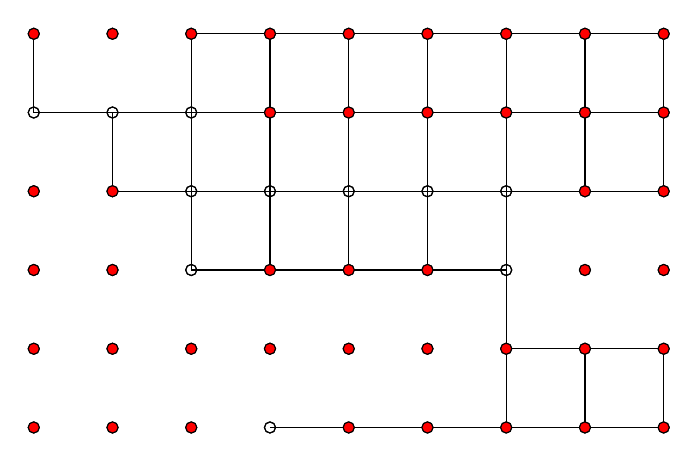
\begin{tikzpicture}[scale=1]%
\path[draw] (0.0,-8.0) -- (1.0,-8.0);%
\path[draw,radius=2pt] (0.0,-8.0) circle;%
\path[draw] (1.0,-8.0) -- (1.0,-9.0);%
\path[draw] (1.0,-8.0) -- (0.0,-8.0);%
\path[draw] (1.0,-8.0) -- (2.0,-8.0);%
\path[draw,radius=2pt] (1.0,-8.0) circle;%
\path[draw] (2.0,-8.0) -- (2.0,-9.0);%
\path[draw] (2.0,-8.0) -- (1.0,-8.0);%
\path[draw,radius=2pt] (2.0,-8.0) circle;%
\path[draw] (1.0,-9.0) -- (1.0,-8.0);%
\path[draw] (1.0,-9.0) -- (2.0,-9.0);%
\path[draw,radius=2pt] (1.0,-9.0) circle;%
\path[draw] (2.0,-9.0) -- (2.0,-8.0);%
\path[draw] (2.0,-9.0) -- (2.0,-10.0);%
\path[draw] (2.0,-9.0) -- (1.0,-9.0);%
\path[draw] (2.0,-9.0) -- (3.0,-9.0);%
\path[draw,radius=2pt] (2.0,-9.0) circle;%
\path[draw] (3.0,-9.0) -- (2.0,-9.0);%
\path[draw] (3.0,-9.0) -- (4.0,-9.0);%
\path[draw,radius=2pt] (3.0,-9.0) circle;%
\path[draw] (4.0,-9.0) -- (3.0,-9.0);%
\path[draw] (4.0,-9.0) -- (5.0,-9.0);%
\path[draw,radius=2pt] (4.0,-9.0) circle;%
\path[draw] (5.0,-9.0) -- (4.0,-9.0);%
\path[draw] (5.0,-9.0) -- (6.0,-9.0);%
\path[draw,radius=2pt] (5.0,-9.0) circle;%
\path[draw] (6.0,-9.0) -- (6.0,-10.0);%
\path[draw] (6.0,-9.0) -- (5.0,-9.0);%
\path[draw,radius=2pt] (6.0,-9.0) circle;%
\path[draw] (2.0,-10.0) -- (2.0,-9.0);%
\path[draw,radius=2pt] (2.0,-10.0) circle;%
\path[draw] (6.0,-10.0) -- (6.0,-9.0);%
\path[draw] (6.0,-10.0) -- (6.0,-11.0);%
\path[draw,radius=2pt] (6.0,-10.0) circle;%
\path[draw] (6.0,-11.0) -- (6.0,-10.0);%
\path[draw] (6.0,-11.0) -- (6.0,-12.0);%
\path[draw] (6.0,-11.0) -- (7.0,-11.0);%
\path[draw,radius=2pt] (6.0,-11.0) circle;%
\path[draw] (7.0,-11.0) -- (7.0,-12.0);%
\path[draw] (7.0,-11.0) -- (6.0,-11.0);%
\path[draw] (7.0,-11.0) -- (8.0,-11.0);%
\path[draw,radius=2pt] (7.0,-11.0) circle;%
\path[draw] (8.0,-11.0) -- (8.0,-12.0);%
\path[draw] (8.0,-11.0) -- (7.0,-11.0);%
\path[draw,radius=2pt] (8.0,-11.0) circle;%
\path[draw] (3.0,-12.0) -- (4.0,-12.0);%
\path[draw,radius=2pt] (3.0,-12.0) circle;%
\path[draw] (4.0,-12.0) -- (3.0,-12.0);%
\path[draw] (4.0,-12.0) -- (5.0,-12.0);%
\path[draw,radius=2pt] (4.0,-12.0) circle;%
\path[draw] (5.0,-12.0) -- (4.0,-12.0);%
\path[draw] (5.0,-12.0) -- (6.0,-12.0);%
\path[draw,radius=2pt] (5.0,-12.0) circle;%
\path[draw] (6.0,-12.0) -- (6.0,-11.0);%
\path[draw] (6.0,-12.0) -- (5.0,-12.0);%
\path[draw] (6.0,-12.0) -- (7.0,-12.0);%
\path[draw,radius=2pt] (6.0,-12.0) circle;%
\path[draw] (7.0,-12.0) -- (7.0,-11.0);%
\path[draw] (7.0,-12.0) -- (6.0,-12.0);%
\path[draw] (7.0,-12.0) -- (8.0,-12.0);%
\path[draw,radius=2pt] (7.0,-12.0) circle;%
\path[draw] (8.0,-12.0) -- (8.0,-11.0);%
\path[draw] (8.0,-12.0) -- (7.0,-12.0);%
\path[draw,radius=2pt] (8.0,-12.0) circle;%
\path[draw] (0.0,-7.0) -- (0.0,-8.0);%
\path[draw,radius=2pt] (0.0,-7.0) circle;%
\path[draw] (2.0,-7.0) -- (2.0,-8.0);%
\path[draw] (2.0,-7.0) -- (3.0,-7.0);%
\path[draw,radius=2pt] (2.0,-7.0) circle;%
\path[draw] (3.0,-7.0) -- (3.0,-8.0);%
\path[draw] (3.0,-7.0) -- (2.0,-7.0);%
\path[draw] (3.0,-7.0) -- (4.0,-7.0);%
\path[draw,radius=2pt] (3.0,-7.0) circle;%
\path[draw] (4.0,-7.0) -- (4.0,-8.0);%
\path[draw] (4.0,-7.0) -- (3.0,-7.0);%
\path[draw] (4.0,-7.0) -- (5.0,-7.0);%
\path[draw,radius=2pt] (4.0,-7.0) circle;%
\path[draw] (5.0,-7.0) -- (5.0,-8.0);%
\path[draw] (5.0,-7.0) -- (4.0,-7.0);%
\path[draw] (5.0,-7.0) -- (6.0,-7.0);%
\path[draw,radius=2pt] (5.0,-7.0) circle;%
\path[draw] (6.0,-7.0) -- (6.0,-8.0);%
\path[draw] (6.0,-7.0) -- (5.0,-7.0);%
\path[draw] (6.0,-7.0) -- (7.0,-7.0);%
\path[draw,radius=2pt] (6.0,-7.0) circle;%
\path[draw] (7.0,-7.0) -- (7.0,-8.0);%
\path[draw] (7.0,-7.0) -- (6.0,-7.0);%
\path[draw] (7.0,-7.0) -- (8.0,-7.0);%
\path[draw,radius=2pt] (7.0,-7.0) circle;%
\path[draw] (8.0,-7.0) -- (8.0,-8.0);%
\path[draw] (8.0,-7.0) -- (7.0,-7.0);%
\path[draw,radius=2pt] (8.0,-7.0) circle;%
\path[draw] (0.0,-8.0) -- (0.0,-7.0);%
\path[draw] (0.0,-8.0) -- (1.0,-8.0);%
\path[draw,radius=2pt] (0.0,-8.0) circle;%
\path[draw] (1.0,-8.0) -- (0.0,-8.0);%
\path[draw] (1.0,-8.0) -- (2.0,-8.0);%
\path[draw,radius=2pt] (1.0,-8.0) circle;%
\path[draw] (2.0,-8.0) -- (2.0,-7.0);%
\path[draw] (2.0,-8.0) -- (2.0,-9.0);%
\path[draw] (2.0,-8.0) -- (1.0,-8.0);%
\path[draw] (2.0,-8.0) -- (3.0,-8.0);%
\path[draw,radius=2pt] (2.0,-8.0) circle;%
\path[draw] (3.0,-8.0) -- (3.0,-7.0);%
\path[draw] (3.0,-8.0) -- (3.0,-9.0);%
\path[draw] (3.0,-8.0) -- (2.0,-8.0);%
\path[draw] (3.0,-8.0) -- (4.0,-8.0);%
\path[draw,radius=2pt] (3.0,-8.0) circle;%
\path[draw] (4.0,-8.0) -- (4.0,-7.0);%
\path[draw] (4.0,-8.0) -- (4.0,-9.0);%
\path[draw] (4.0,-8.0) -- (3.0,-8.0);%
\path[draw] (4.0,-8.0) -- (5.0,-8.0);%
\path[draw,radius=2pt] (4.0,-8.0) circle;%
\path[draw] (5.0,-8.0) -- (5.0,-7.0);%
\path[draw] (5.0,-8.0) -- (5.0,-9.0);%
\path[draw] (5.0,-8.0) -- (4.0,-8.0);%
\path[draw] (5.0,-8.0) -- (6.0,-8.0);%
\path[draw,radius=2pt] (5.0,-8.0) circle;%
\path[draw] (6.0,-8.0) -- (6.0,-7.0);%
\path[draw] (6.0,-8.0) -- (6.0,-9.0);%
\path[draw] (6.0,-8.0) -- (5.0,-8.0);%
\path[draw] (6.0,-8.0) -- (7.0,-8.0);%
\path[draw,radius=2pt] (6.0,-8.0) circle;%
\path[draw] (7.0,-8.0) -- (7.0,-7.0);%
\path[draw] (7.0,-8.0) -- (7.0,-9.0);%
\path[draw] (7.0,-8.0) -- (6.0,-8.0);%
\path[draw] (7.0,-8.0) -- (8.0,-8.0);%
\path[draw,radius=2pt] (7.0,-8.0) circle;%
\path[draw] (8.0,-8.0) -- (8.0,-7.0);%
\path[draw] (8.0,-8.0) -- (8.0,-9.0);%
\path[draw] (8.0,-8.0) -- (7.0,-8.0);%
\path[draw,radius=2pt] (8.0,-8.0) circle;%
\path[draw] (2.0,-9.0) -- (2.0,-8.0);%
\path[draw] (2.0,-9.0) -- (2.0,-10.0);%
\path[draw] (2.0,-9.0) -- (3.0,-9.0);%
\path[draw,radius=2pt] (2.0,-9.0) circle;%
\path[draw] (3.0,-9.0) -- (3.0,-8.0);%
\path[draw] (3.0,-9.0) -- (3.0,-10.0);%
\path[draw] (3.0,-9.0) -- (2.0,-9.0);%
\path[draw] (3.0,-9.0) -- (4.0,-9.0);%
\path[draw,radius=2pt] (3.0,-9.0) circle;%
\path[draw] (4.0,-9.0) -- (4.0,-8.0);%
\path[draw] (4.0,-9.0) -- (4.0,-10.0);%
\path[draw] (4.0,-9.0) -- (3.0,-9.0);%
\path[draw] (4.0,-9.0) -- (5.0,-9.0);%
\path[draw,radius=2pt] (4.0,-9.0) circle;%
\path[draw] (5.0,-9.0) -- (5.0,-8.0);%
\path[draw] (5.0,-9.0) -- (5.0,-10.0);%
\path[draw] (5.0,-9.0) -- (4.0,-9.0);%
\path[draw] (5.0,-9.0) -- (6.0,-9.0);%
\path[draw,radius=2pt] (5.0,-9.0) circle;%
\path[draw] (6.0,-9.0) -- (6.0,-8.0);%
\path[draw] (6.0,-9.0) -- (6.0,-10.0);%
\path[draw] (6.0,-9.0) -- (5.0,-9.0);%
\path[draw] (6.0,-9.0) -- (7.0,-9.0);%
\path[draw,radius=2pt] (6.0,-9.0) circle;%
\path[draw] (7.0,-9.0) -- (7.0,-8.0);%
\path[draw] (7.0,-9.0) -- (6.0,-9.0);%
\path[draw] (7.0,-9.0) -- (8.0,-9.0);%
\path[draw,radius=2pt] (7.0,-9.0) circle;%
\path[draw] (8.0,-9.0) -- (8.0,-8.0);%
\path[draw] (8.0,-9.0) -- (7.0,-9.0);%
\path[draw,radius=2pt] (8.0,-9.0) circle;%
\path[draw] (2.0,-10.0) -- (2.0,-9.0);%
\path[draw] (2.0,-10.0) -- (3.0,-10.0);%
\path[draw,radius=2pt] (2.0,-10.0) circle;%
\path[draw] (3.0,-10.0) -- (3.0,-9.0);%
\path[draw] (3.0,-10.0) -- (2.0,-10.0);%
\path[draw] (3.0,-10.0) -- (4.0,-10.0);%
\path[draw,radius=2pt] (3.0,-10.0) circle;%
\path[draw] (4.0,-10.0) -- (4.0,-9.0);%
\path[draw] (4.0,-10.0) -- (3.0,-10.0);%
\path[draw] (4.0,-10.0) -- (5.0,-10.0);%
\path[draw,radius=2pt] (4.0,-10.0) circle;%
\path[draw] (5.0,-10.0) -- (5.0,-9.0);%
\path[draw] (5.0,-10.0) -- (4.0,-10.0);%
\path[draw] (5.0,-10.0) -- (6.0,-10.0);%
\path[draw,radius=2pt] (5.0,-10.0) circle;%
\path[draw] (6.0,-10.0) -- (6.0,-9.0);%
\path[draw] (6.0,-10.0) -- (5.0,-10.0);%
\path[draw,radius=2pt] (6.0,-10.0) circle;%
\path[draw,radius=2pt] (3.0,-12.0) circle;%
\path[draw,radius=2pt,fill=red] (0.0,-7.0) circle;%
\path[draw,radius=2pt,fill=red] (1.0,-7.0) circle;%
\path[draw,radius=2pt,fill=red] (2.0,-7.0) circle;%
\path[draw,radius=2pt,fill=red] (3.0,-7.0) circle;%
\path[draw,radius=2pt,fill=red] (4.0,-7.0) circle;%
\path[draw,radius=2pt,fill=red] (5.0,-7.0) circle;%
\path[draw,radius=2pt,fill=red] (6.0,-7.0) circle;%
\path[draw,radius=2pt,fill=red] (7.0,-7.0) circle;%
\path[draw,radius=2pt,fill=red] (8.0,-7.0) circle;%
\path[draw,radius=2pt,fill=red] (3.0,-8.0) circle;%
\path[draw,radius=2pt,fill=red] (4.0,-8.0) circle;%
\path[draw,radius=2pt,fill=red] (5.0,-8.0) circle;%
\path[draw,radius=2pt,fill=red] (6.0,-8.0) circle;%
\path[draw,radius=2pt,fill=red] (7.0,-8.0) circle;%
\path[draw,radius=2pt,fill=red] (8.0,-8.0) circle;%
\path[draw,radius=2pt,fill=red] (0.0,-9.0) circle;%
\path[draw,radius=2pt,fill=red] (7.0,-9.0) circle;%
\path[draw,radius=2pt,fill=red] (8.0,-9.0) circle;%
\path[draw,radius=2pt,fill=red] (0.0,-10.0) circle;%
\path[draw,radius=2pt,fill=red] (1.0,-10.0) circle;%
\path[draw,radius=2pt,fill=red] (3.0,-10.0) circle;%
\path[draw,radius=2pt,fill=red] (4.0,-10.0) circle;%
\path[draw,radius=2pt,fill=red] (5.0,-10.0) circle;%
\path[draw,radius=2pt,fill=red] (7.0,-10.0) circle;%
\path[draw,radius=2pt,fill=red] (8.0,-10.0) circle;%
\path[draw,radius=2pt,fill=red] (0.0,-11.0) circle;%
\path[draw,radius=2pt,fill=red] (1.0,-11.0) circle;%
\path[draw,radius=2pt,fill=red] (2.0,-11.0) circle;%
\path[draw,radius=2pt,fill=red] (3.0,-11.0) circle;%
\path[draw,radius=2pt,fill=red] (4.0,-11.0) circle;%
\path[draw,radius=2pt,fill=red] (5.0,-11.0) circle;%
\path[draw,radius=2pt,fill=red] (0.0,-12.0) circle;%
\path[draw,radius=2pt,fill=red] (1.0,-12.0) circle;%
\path[draw,radius=2pt,fill=red] (2.0,-12.0) circle;%
\path[draw,radius=2pt,fill=red] (1.0,-7.0) circle;%
\path[draw,radius=2pt,fill=red] (0.0,-9.0) circle;%
\path[draw,radius=2pt,fill=red] (1.0,-9.0) circle;%
\path[draw,radius=2pt,fill=red] (0.0,-10.0) circle;%
\path[draw,radius=2pt,fill=red] (1.0,-10.0) circle;%
\path[draw,radius=2pt,fill=red] (7.0,-10.0) circle;%
\path[draw,radius=2pt,fill=red] (8.0,-10.0) circle;%
\path[draw,radius=2pt,fill=red] (0.0,-11.0) circle;%
\path[draw,radius=2pt,fill=red] (1.0,-11.0) circle;%
\path[draw,radius=2pt,fill=red] (2.0,-11.0) circle;%
\path[draw,radius=2pt,fill=red] (3.0,-11.0) circle;%
\path[draw,radius=2pt,fill=red] (4.0,-11.0) circle;%
\path[draw,radius=2pt,fill=red] (5.0,-11.0) circle;%
\path[draw,radius=2pt,fill=red] (6.0,-11.0) circle;%
\path[draw,radius=2pt,fill=red] (7.0,-11.0) circle;%
\path[draw,radius=2pt,fill=red] (8.0,-11.0) circle;%
\path[draw,radius=2pt,fill=red] (0.0,-12.0) circle;%
\path[draw,radius=2pt,fill=red] (1.0,-12.0) circle;%
\path[draw,radius=2pt,fill=red] (2.0,-12.0) circle;%
\path[draw,radius=2pt,fill=red] (4.0,-12.0) circle;%
\path[draw,radius=2pt,fill=red] (5.0,-12.0) circle;%
\path[draw,radius=2pt,fill=red] (6.0,-12.0) circle;%
\path[draw,radius=2pt,fill=red] (7.0,-12.0) circle;%
\path[draw,radius=2pt,fill=red] (8.0,-12.0) circle;%
\end{tikzpicture}%
\newline%
\hspace*{1in}%
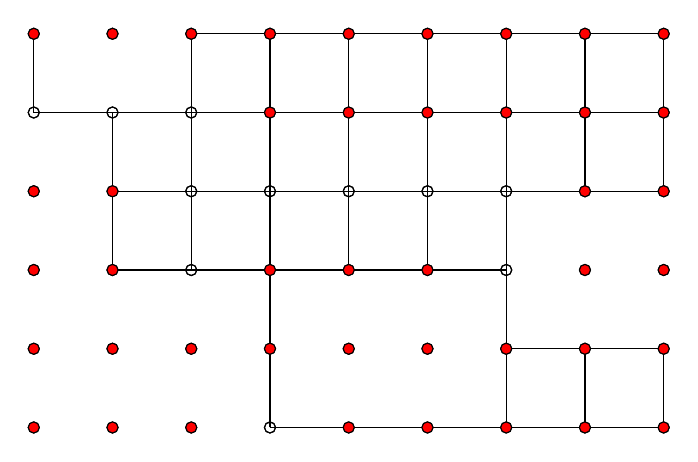
\begin{tikzpicture}[scale=1]%
\path[draw] (0.0,-8.0) -- (1.0,-8.0);%
\path[draw,radius=2pt] (0.0,-8.0) circle;%
\path[draw] (1.0,-8.0) -- (1.0,-9.0);%
\path[draw] (1.0,-8.0) -- (0.0,-8.0);%
\path[draw] (1.0,-8.0) -- (2.0,-8.0);%
\path[draw,radius=2pt] (1.0,-8.0) circle;%
\path[draw] (2.0,-8.0) -- (2.0,-9.0);%
\path[draw] (2.0,-8.0) -- (1.0,-8.0);%
\path[draw,radius=2pt] (2.0,-8.0) circle;%
\path[draw] (1.0,-9.0) -- (1.0,-8.0);%
\path[draw] (1.0,-9.0) -- (1.0,-10.0);%
\path[draw] (1.0,-9.0) -- (2.0,-9.0);%
\path[draw,radius=2pt] (1.0,-9.0) circle;%
\path[draw] (2.0,-9.0) -- (2.0,-8.0);%
\path[draw] (2.0,-9.0) -- (2.0,-10.0);%
\path[draw] (2.0,-9.0) -- (1.0,-9.0);%
\path[draw] (2.0,-9.0) -- (3.0,-9.0);%
\path[draw,radius=2pt] (2.0,-9.0) circle;%
\path[draw] (3.0,-9.0) -- (2.0,-9.0);%
\path[draw] (3.0,-9.0) -- (4.0,-9.0);%
\path[draw,radius=2pt] (3.0,-9.0) circle;%
\path[draw] (4.0,-9.0) -- (3.0,-9.0);%
\path[draw] (4.0,-9.0) -- (5.0,-9.0);%
\path[draw,radius=2pt] (4.0,-9.0) circle;%
\path[draw] (5.0,-9.0) -- (4.0,-9.0);%
\path[draw] (5.0,-9.0) -- (6.0,-9.0);%
\path[draw,radius=2pt] (5.0,-9.0) circle;%
\path[draw] (6.0,-9.0) -- (6.0,-10.0);%
\path[draw] (6.0,-9.0) -- (5.0,-9.0);%
\path[draw,radius=2pt] (6.0,-9.0) circle;%
\path[draw] (1.0,-10.0) -- (1.0,-9.0);%
\path[draw] (1.0,-10.0) -- (2.0,-10.0);%
\path[draw,radius=2pt] (1.0,-10.0) circle;%
\path[draw] (2.0,-10.0) -- (2.0,-9.0);%
\path[draw] (2.0,-10.0) -- (1.0,-10.0);%
\path[draw,radius=2pt] (2.0,-10.0) circle;%
\path[draw] (6.0,-10.0) -- (6.0,-9.0);%
\path[draw] (6.0,-10.0) -- (6.0,-11.0);%
\path[draw,radius=2pt] (6.0,-10.0) circle;%
\path[draw] (6.0,-11.0) -- (6.0,-10.0);%
\path[draw] (6.0,-11.0) -- (6.0,-12.0);%
\path[draw] (6.0,-11.0) -- (7.0,-11.0);%
\path[draw,radius=2pt] (6.0,-11.0) circle;%
\path[draw] (7.0,-11.0) -- (7.0,-12.0);%
\path[draw] (7.0,-11.0) -- (6.0,-11.0);%
\path[draw] (7.0,-11.0) -- (8.0,-11.0);%
\path[draw,radius=2pt] (7.0,-11.0) circle;%
\path[draw] (8.0,-11.0) -- (8.0,-12.0);%
\path[draw] (8.0,-11.0) -- (7.0,-11.0);%
\path[draw,radius=2pt] (8.0,-11.0) circle;%
\path[draw] (3.0,-12.0) -- (4.0,-12.0);%
\path[draw,radius=2pt] (3.0,-12.0) circle;%
\path[draw] (4.0,-12.0) -- (3.0,-12.0);%
\path[draw] (4.0,-12.0) -- (5.0,-12.0);%
\path[draw,radius=2pt] (4.0,-12.0) circle;%
\path[draw] (5.0,-12.0) -- (4.0,-12.0);%
\path[draw] (5.0,-12.0) -- (6.0,-12.0);%
\path[draw,radius=2pt] (5.0,-12.0) circle;%
\path[draw] (6.0,-12.0) -- (6.0,-11.0);%
\path[draw] (6.0,-12.0) -- (5.0,-12.0);%
\path[draw] (6.0,-12.0) -- (7.0,-12.0);%
\path[draw,radius=2pt] (6.0,-12.0) circle;%
\path[draw] (7.0,-12.0) -- (7.0,-11.0);%
\path[draw] (7.0,-12.0) -- (6.0,-12.0);%
\path[draw] (7.0,-12.0) -- (8.0,-12.0);%
\path[draw,radius=2pt] (7.0,-12.0) circle;%
\path[draw] (8.0,-12.0) -- (8.0,-11.0);%
\path[draw] (8.0,-12.0) -- (7.0,-12.0);%
\path[draw,radius=2pt] (8.0,-12.0) circle;%
\path[draw] (0.0,-7.0) -- (0.0,-8.0);%
\path[draw,radius=2pt] (0.0,-7.0) circle;%
\path[draw] (2.0,-7.0) -- (2.0,-8.0);%
\path[draw] (2.0,-7.0) -- (3.0,-7.0);%
\path[draw,radius=2pt] (2.0,-7.0) circle;%
\path[draw] (3.0,-7.0) -- (3.0,-8.0);%
\path[draw] (3.0,-7.0) -- (2.0,-7.0);%
\path[draw] (3.0,-7.0) -- (4.0,-7.0);%
\path[draw,radius=2pt] (3.0,-7.0) circle;%
\path[draw] (4.0,-7.0) -- (4.0,-8.0);%
\path[draw] (4.0,-7.0) -- (3.0,-7.0);%
\path[draw] (4.0,-7.0) -- (5.0,-7.0);%
\path[draw,radius=2pt] (4.0,-7.0) circle;%
\path[draw] (5.0,-7.0) -- (5.0,-8.0);%
\path[draw] (5.0,-7.0) -- (4.0,-7.0);%
\path[draw] (5.0,-7.0) -- (6.0,-7.0);%
\path[draw,radius=2pt] (5.0,-7.0) circle;%
\path[draw] (6.0,-7.0) -- (6.0,-8.0);%
\path[draw] (6.0,-7.0) -- (5.0,-7.0);%
\path[draw] (6.0,-7.0) -- (7.0,-7.0);%
\path[draw,radius=2pt] (6.0,-7.0) circle;%
\path[draw] (7.0,-7.0) -- (7.0,-8.0);%
\path[draw] (7.0,-7.0) -- (6.0,-7.0);%
\path[draw] (7.0,-7.0) -- (8.0,-7.0);%
\path[draw,radius=2pt] (7.0,-7.0) circle;%
\path[draw] (8.0,-7.0) -- (8.0,-8.0);%
\path[draw] (8.0,-7.0) -- (7.0,-7.0);%
\path[draw,radius=2pt] (8.0,-7.0) circle;%
\path[draw] (0.0,-8.0) -- (0.0,-7.0);%
\path[draw] (0.0,-8.0) -- (1.0,-8.0);%
\path[draw,radius=2pt] (0.0,-8.0) circle;%
\path[draw] (1.0,-8.0) -- (0.0,-8.0);%
\path[draw] (1.0,-8.0) -- (2.0,-8.0);%
\path[draw,radius=2pt] (1.0,-8.0) circle;%
\path[draw] (2.0,-8.0) -- (2.0,-7.0);%
\path[draw] (2.0,-8.0) -- (2.0,-9.0);%
\path[draw] (2.0,-8.0) -- (1.0,-8.0);%
\path[draw] (2.0,-8.0) -- (3.0,-8.0);%
\path[draw,radius=2pt] (2.0,-8.0) circle;%
\path[draw] (3.0,-8.0) -- (3.0,-7.0);%
\path[draw] (3.0,-8.0) -- (3.0,-9.0);%
\path[draw] (3.0,-8.0) -- (2.0,-8.0);%
\path[draw] (3.0,-8.0) -- (4.0,-8.0);%
\path[draw,radius=2pt] (3.0,-8.0) circle;%
\path[draw] (4.0,-8.0) -- (4.0,-7.0);%
\path[draw] (4.0,-8.0) -- (4.0,-9.0);%
\path[draw] (4.0,-8.0) -- (3.0,-8.0);%
\path[draw] (4.0,-8.0) -- (5.0,-8.0);%
\path[draw,radius=2pt] (4.0,-8.0) circle;%
\path[draw] (5.0,-8.0) -- (5.0,-7.0);%
\path[draw] (5.0,-8.0) -- (5.0,-9.0);%
\path[draw] (5.0,-8.0) -- (4.0,-8.0);%
\path[draw] (5.0,-8.0) -- (6.0,-8.0);%
\path[draw,radius=2pt] (5.0,-8.0) circle;%
\path[draw] (6.0,-8.0) -- (6.0,-7.0);%
\path[draw] (6.0,-8.0) -- (6.0,-9.0);%
\path[draw] (6.0,-8.0) -- (5.0,-8.0);%
\path[draw] (6.0,-8.0) -- (7.0,-8.0);%
\path[draw,radius=2pt] (6.0,-8.0) circle;%
\path[draw] (7.0,-8.0) -- (7.0,-7.0);%
\path[draw] (7.0,-8.0) -- (7.0,-9.0);%
\path[draw] (7.0,-8.0) -- (6.0,-8.0);%
\path[draw] (7.0,-8.0) -- (8.0,-8.0);%
\path[draw,radius=2pt] (7.0,-8.0) circle;%
\path[draw] (8.0,-8.0) -- (8.0,-7.0);%
\path[draw] (8.0,-8.0) -- (8.0,-9.0);%
\path[draw] (8.0,-8.0) -- (7.0,-8.0);%
\path[draw,radius=2pt] (8.0,-8.0) circle;%
\path[draw] (2.0,-9.0) -- (2.0,-8.0);%
\path[draw] (2.0,-9.0) -- (2.0,-10.0);%
\path[draw] (2.0,-9.0) -- (3.0,-9.0);%
\path[draw,radius=2pt] (2.0,-9.0) circle;%
\path[draw] (3.0,-9.0) -- (3.0,-8.0);%
\path[draw] (3.0,-9.0) -- (3.0,-10.0);%
\path[draw] (3.0,-9.0) -- (2.0,-9.0);%
\path[draw] (3.0,-9.0) -- (4.0,-9.0);%
\path[draw,radius=2pt] (3.0,-9.0) circle;%
\path[draw] (4.0,-9.0) -- (4.0,-8.0);%
\path[draw] (4.0,-9.0) -- (4.0,-10.0);%
\path[draw] (4.0,-9.0) -- (3.0,-9.0);%
\path[draw] (4.0,-9.0) -- (5.0,-9.0);%
\path[draw,radius=2pt] (4.0,-9.0) circle;%
\path[draw] (5.0,-9.0) -- (5.0,-8.0);%
\path[draw] (5.0,-9.0) -- (5.0,-10.0);%
\path[draw] (5.0,-9.0) -- (4.0,-9.0);%
\path[draw] (5.0,-9.0) -- (6.0,-9.0);%
\path[draw,radius=2pt] (5.0,-9.0) circle;%
\path[draw] (6.0,-9.0) -- (6.0,-8.0);%
\path[draw] (6.0,-9.0) -- (6.0,-10.0);%
\path[draw] (6.0,-9.0) -- (5.0,-9.0);%
\path[draw] (6.0,-9.0) -- (7.0,-9.0);%
\path[draw,radius=2pt] (6.0,-9.0) circle;%
\path[draw] (7.0,-9.0) -- (7.0,-8.0);%
\path[draw] (7.0,-9.0) -- (6.0,-9.0);%
\path[draw] (7.0,-9.0) -- (8.0,-9.0);%
\path[draw,radius=2pt] (7.0,-9.0) circle;%
\path[draw] (8.0,-9.0) -- (8.0,-8.0);%
\path[draw] (8.0,-9.0) -- (7.0,-9.0);%
\path[draw,radius=2pt] (8.0,-9.0) circle;%
\path[draw] (2.0,-10.0) -- (2.0,-9.0);%
\path[draw] (2.0,-10.0) -- (3.0,-10.0);%
\path[draw,radius=2pt] (2.0,-10.0) circle;%
\path[draw] (3.0,-10.0) -- (3.0,-9.0);%
\path[draw] (3.0,-10.0) -- (3.0,-11.0);%
\path[draw] (3.0,-10.0) -- (2.0,-10.0);%
\path[draw] (3.0,-10.0) -- (4.0,-10.0);%
\path[draw,radius=2pt] (3.0,-10.0) circle;%
\path[draw] (4.0,-10.0) -- (4.0,-9.0);%
\path[draw] (4.0,-10.0) -- (3.0,-10.0);%
\path[draw] (4.0,-10.0) -- (5.0,-10.0);%
\path[draw,radius=2pt] (4.0,-10.0) circle;%
\path[draw] (5.0,-10.0) -- (5.0,-9.0);%
\path[draw] (5.0,-10.0) -- (4.0,-10.0);%
\path[draw] (5.0,-10.0) -- (6.0,-10.0);%
\path[draw,radius=2pt] (5.0,-10.0) circle;%
\path[draw] (6.0,-10.0) -- (6.0,-9.0);%
\path[draw] (6.0,-10.0) -- (5.0,-10.0);%
\path[draw,radius=2pt] (6.0,-10.0) circle;%
\path[draw] (3.0,-11.0) -- (3.0,-10.0);%
\path[draw] (3.0,-11.0) -- (3.0,-12.0);%
\path[draw,radius=2pt] (3.0,-11.0) circle;%
\path[draw] (3.0,-12.0) -- (3.0,-11.0);%
\path[draw,radius=2pt] (3.0,-12.0) circle;%
\path[draw,radius=2pt,fill=red] (0.0,-7.0) circle;%
\path[draw,radius=2pt,fill=red] (1.0,-7.0) circle;%
\path[draw,radius=2pt,fill=red] (2.0,-7.0) circle;%
\path[draw,radius=2pt,fill=red] (3.0,-7.0) circle;%
\path[draw,radius=2pt,fill=red] (4.0,-7.0) circle;%
\path[draw,radius=2pt,fill=red] (5.0,-7.0) circle;%
\path[draw,radius=2pt,fill=red] (6.0,-7.0) circle;%
\path[draw,radius=2pt,fill=red] (7.0,-7.0) circle;%
\path[draw,radius=2pt,fill=red] (8.0,-7.0) circle;%
\path[draw,radius=2pt,fill=red] (3.0,-8.0) circle;%
\path[draw,radius=2pt,fill=red] (4.0,-8.0) circle;%
\path[draw,radius=2pt,fill=red] (5.0,-8.0) circle;%
\path[draw,radius=2pt,fill=red] (6.0,-8.0) circle;%
\path[draw,radius=2pt,fill=red] (7.0,-8.0) circle;%
\path[draw,radius=2pt,fill=red] (8.0,-8.0) circle;%
\path[draw,radius=2pt,fill=red] (0.0,-9.0) circle;%
\path[draw,radius=2pt,fill=red] (7.0,-9.0) circle;%
\path[draw,radius=2pt,fill=red] (8.0,-9.0) circle;%
\path[draw,radius=2pt,fill=red] (0.0,-10.0) circle;%
\path[draw,radius=2pt,fill=red] (3.0,-10.0) circle;%
\path[draw,radius=2pt,fill=red] (4.0,-10.0) circle;%
\path[draw,radius=2pt,fill=red] (5.0,-10.0) circle;%
\path[draw,radius=2pt,fill=red] (7.0,-10.0) circle;%
\path[draw,radius=2pt,fill=red] (8.0,-10.0) circle;%
\path[draw,radius=2pt,fill=red] (0.0,-11.0) circle;%
\path[draw,radius=2pt,fill=red] (1.0,-11.0) circle;%
\path[draw,radius=2pt,fill=red] (2.0,-11.0) circle;%
\path[draw,radius=2pt,fill=red] (3.0,-11.0) circle;%
\path[draw,radius=2pt,fill=red] (4.0,-11.0) circle;%
\path[draw,radius=2pt,fill=red] (5.0,-11.0) circle;%
\path[draw,radius=2pt,fill=red] (0.0,-12.0) circle;%
\path[draw,radius=2pt,fill=red] (1.0,-12.0) circle;%
\path[draw,radius=2pt,fill=red] (2.0,-12.0) circle;%
\path[draw,radius=2pt,fill=red] (1.0,-7.0) circle;%
\path[draw,radius=2pt,fill=red] (0.0,-9.0) circle;%
\path[draw,radius=2pt,fill=red] (1.0,-9.0) circle;%
\path[draw,radius=2pt,fill=red] (0.0,-10.0) circle;%
\path[draw,radius=2pt,fill=red] (1.0,-10.0) circle;%
\path[draw,radius=2pt,fill=red] (7.0,-10.0) circle;%
\path[draw,radius=2pt,fill=red] (8.0,-10.0) circle;%
\path[draw,radius=2pt,fill=red] (0.0,-11.0) circle;%
\path[draw,radius=2pt,fill=red] (1.0,-11.0) circle;%
\path[draw,radius=2pt,fill=red] (2.0,-11.0) circle;%
\path[draw,radius=2pt,fill=red] (4.0,-11.0) circle;%
\path[draw,radius=2pt,fill=red] (5.0,-11.0) circle;%
\path[draw,radius=2pt,fill=red] (6.0,-11.0) circle;%
\path[draw,radius=2pt,fill=red] (7.0,-11.0) circle;%
\path[draw,radius=2pt,fill=red] (8.0,-11.0) circle;%
\path[draw,radius=2pt,fill=red] (0.0,-12.0) circle;%
\path[draw,radius=2pt,fill=red] (1.0,-12.0) circle;%
\path[draw,radius=2pt,fill=red] (2.0,-12.0) circle;%
\path[draw,radius=2pt,fill=red] (4.0,-12.0) circle;%
\path[draw,radius=2pt,fill=red] (5.0,-12.0) circle;%
\path[draw,radius=2pt,fill=red] (6.0,-12.0) circle;%
\path[draw,radius=2pt,fill=red] (7.0,-12.0) circle;%
\path[draw,radius=2pt,fill=red] (8.0,-12.0) circle;%
\end{tikzpicture}%
\hspace*{1in}%
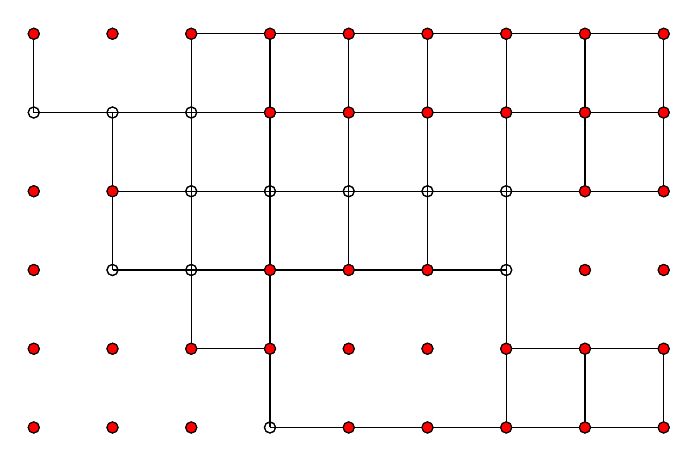
\begin{tikzpicture}[scale=1]%
\path[draw] (0.0,-8.0) -- (1.0,-8.0);%
\path[draw,radius=2pt] (0.0,-8.0) circle;%
\path[draw] (1.0,-8.0) -- (1.0,-9.0);%
\path[draw] (1.0,-8.0) -- (0.0,-8.0);%
\path[draw] (1.0,-8.0) -- (2.0,-8.0);%
\path[draw,radius=2pt] (1.0,-8.0) circle;%
\path[draw] (2.0,-8.0) -- (2.0,-9.0);%
\path[draw] (2.0,-8.0) -- (1.0,-8.0);%
\path[draw,radius=2pt] (2.0,-8.0) circle;%
\path[draw] (1.0,-9.0) -- (1.0,-8.0);%
\path[draw] (1.0,-9.0) -- (1.0,-10.0);%
\path[draw] (1.0,-9.0) -- (2.0,-9.0);%
\path[draw,radius=2pt] (1.0,-9.0) circle;%
\path[draw] (2.0,-9.0) -- (2.0,-8.0);%
\path[draw] (2.0,-9.0) -- (2.0,-10.0);%
\path[draw] (2.0,-9.0) -- (1.0,-9.0);%
\path[draw] (2.0,-9.0) -- (3.0,-9.0);%
\path[draw,radius=2pt] (2.0,-9.0) circle;%
\path[draw] (3.0,-9.0) -- (2.0,-9.0);%
\path[draw] (3.0,-9.0) -- (4.0,-9.0);%
\path[draw,radius=2pt] (3.0,-9.0) circle;%
\path[draw] (4.0,-9.0) -- (3.0,-9.0);%
\path[draw] (4.0,-9.0) -- (5.0,-9.0);%
\path[draw,radius=2pt] (4.0,-9.0) circle;%
\path[draw] (5.0,-9.0) -- (4.0,-9.0);%
\path[draw] (5.0,-9.0) -- (6.0,-9.0);%
\path[draw,radius=2pt] (5.0,-9.0) circle;%
\path[draw] (6.0,-9.0) -- (6.0,-10.0);%
\path[draw] (6.0,-9.0) -- (5.0,-9.0);%
\path[draw,radius=2pt] (6.0,-9.0) circle;%
\path[draw] (1.0,-10.0) -- (1.0,-9.0);%
\path[draw] (1.0,-10.0) -- (2.0,-10.0);%
\path[draw,radius=2pt] (1.0,-10.0) circle;%
\path[draw] (2.0,-10.0) -- (2.0,-9.0);%
\path[draw] (2.0,-10.0) -- (1.0,-10.0);%
\path[draw,radius=2pt] (2.0,-10.0) circle;%
\path[draw] (6.0,-10.0) -- (6.0,-9.0);%
\path[draw] (6.0,-10.0) -- (6.0,-11.0);%
\path[draw,radius=2pt] (6.0,-10.0) circle;%
\path[draw] (6.0,-11.0) -- (6.0,-10.0);%
\path[draw] (6.0,-11.0) -- (6.0,-12.0);%
\path[draw] (6.0,-11.0) -- (7.0,-11.0);%
\path[draw,radius=2pt] (6.0,-11.0) circle;%
\path[draw] (7.0,-11.0) -- (7.0,-12.0);%
\path[draw] (7.0,-11.0) -- (6.0,-11.0);%
\path[draw] (7.0,-11.0) -- (8.0,-11.0);%
\path[draw,radius=2pt] (7.0,-11.0) circle;%
\path[draw] (8.0,-11.0) -- (8.0,-12.0);%
\path[draw] (8.0,-11.0) -- (7.0,-11.0);%
\path[draw,radius=2pt] (8.0,-11.0) circle;%
\path[draw] (3.0,-12.0) -- (4.0,-12.0);%
\path[draw,radius=2pt] (3.0,-12.0) circle;%
\path[draw] (4.0,-12.0) -- (3.0,-12.0);%
\path[draw] (4.0,-12.0) -- (5.0,-12.0);%
\path[draw,radius=2pt] (4.0,-12.0) circle;%
\path[draw] (5.0,-12.0) -- (4.0,-12.0);%
\path[draw] (5.0,-12.0) -- (6.0,-12.0);%
\path[draw,radius=2pt] (5.0,-12.0) circle;%
\path[draw] (6.0,-12.0) -- (6.0,-11.0);%
\path[draw] (6.0,-12.0) -- (5.0,-12.0);%
\path[draw] (6.0,-12.0) -- (7.0,-12.0);%
\path[draw,radius=2pt] (6.0,-12.0) circle;%
\path[draw] (7.0,-12.0) -- (7.0,-11.0);%
\path[draw] (7.0,-12.0) -- (6.0,-12.0);%
\path[draw] (7.0,-12.0) -- (8.0,-12.0);%
\path[draw,radius=2pt] (7.0,-12.0) circle;%
\path[draw] (8.0,-12.0) -- (8.0,-11.0);%
\path[draw] (8.0,-12.0) -- (7.0,-12.0);%
\path[draw,radius=2pt] (8.0,-12.0) circle;%
\path[draw] (0.0,-7.0) -- (0.0,-8.0);%
\path[draw,radius=2pt] (0.0,-7.0) circle;%
\path[draw] (2.0,-7.0) -- (2.0,-8.0);%
\path[draw] (2.0,-7.0) -- (3.0,-7.0);%
\path[draw,radius=2pt] (2.0,-7.0) circle;%
\path[draw] (3.0,-7.0) -- (3.0,-8.0);%
\path[draw] (3.0,-7.0) -- (2.0,-7.0);%
\path[draw] (3.0,-7.0) -- (4.0,-7.0);%
\path[draw,radius=2pt] (3.0,-7.0) circle;%
\path[draw] (4.0,-7.0) -- (4.0,-8.0);%
\path[draw] (4.0,-7.0) -- (3.0,-7.0);%
\path[draw] (4.0,-7.0) -- (5.0,-7.0);%
\path[draw,radius=2pt] (4.0,-7.0) circle;%
\path[draw] (5.0,-7.0) -- (5.0,-8.0);%
\path[draw] (5.0,-7.0) -- (4.0,-7.0);%
\path[draw] (5.0,-7.0) -- (6.0,-7.0);%
\path[draw,radius=2pt] (5.0,-7.0) circle;%
\path[draw] (6.0,-7.0) -- (6.0,-8.0);%
\path[draw] (6.0,-7.0) -- (5.0,-7.0);%
\path[draw] (6.0,-7.0) -- (7.0,-7.0);%
\path[draw,radius=2pt] (6.0,-7.0) circle;%
\path[draw] (7.0,-7.0) -- (7.0,-8.0);%
\path[draw] (7.0,-7.0) -- (6.0,-7.0);%
\path[draw] (7.0,-7.0) -- (8.0,-7.0);%
\path[draw,radius=2pt] (7.0,-7.0) circle;%
\path[draw] (8.0,-7.0) -- (8.0,-8.0);%
\path[draw] (8.0,-7.0) -- (7.0,-7.0);%
\path[draw,radius=2pt] (8.0,-7.0) circle;%
\path[draw] (0.0,-8.0) -- (0.0,-7.0);%
\path[draw] (0.0,-8.0) -- (1.0,-8.0);%
\path[draw,radius=2pt] (0.0,-8.0) circle;%
\path[draw] (1.0,-8.0) -- (0.0,-8.0);%
\path[draw] (1.0,-8.0) -- (2.0,-8.0);%
\path[draw,radius=2pt] (1.0,-8.0) circle;%
\path[draw] (2.0,-8.0) -- (2.0,-7.0);%
\path[draw] (2.0,-8.0) -- (2.0,-9.0);%
\path[draw] (2.0,-8.0) -- (1.0,-8.0);%
\path[draw] (2.0,-8.0) -- (3.0,-8.0);%
\path[draw,radius=2pt] (2.0,-8.0) circle;%
\path[draw] (3.0,-8.0) -- (3.0,-7.0);%
\path[draw] (3.0,-8.0) -- (3.0,-9.0);%
\path[draw] (3.0,-8.0) -- (2.0,-8.0);%
\path[draw] (3.0,-8.0) -- (4.0,-8.0);%
\path[draw,radius=2pt] (3.0,-8.0) circle;%
\path[draw] (4.0,-8.0) -- (4.0,-7.0);%
\path[draw] (4.0,-8.0) -- (4.0,-9.0);%
\path[draw] (4.0,-8.0) -- (3.0,-8.0);%
\path[draw] (4.0,-8.0) -- (5.0,-8.0);%
\path[draw,radius=2pt] (4.0,-8.0) circle;%
\path[draw] (5.0,-8.0) -- (5.0,-7.0);%
\path[draw] (5.0,-8.0) -- (5.0,-9.0);%
\path[draw] (5.0,-8.0) -- (4.0,-8.0);%
\path[draw] (5.0,-8.0) -- (6.0,-8.0);%
\path[draw,radius=2pt] (5.0,-8.0) circle;%
\path[draw] (6.0,-8.0) -- (6.0,-7.0);%
\path[draw] (6.0,-8.0) -- (6.0,-9.0);%
\path[draw] (6.0,-8.0) -- (5.0,-8.0);%
\path[draw] (6.0,-8.0) -- (7.0,-8.0);%
\path[draw,radius=2pt] (6.0,-8.0) circle;%
\path[draw] (7.0,-8.0) -- (7.0,-7.0);%
\path[draw] (7.0,-8.0) -- (7.0,-9.0);%
\path[draw] (7.0,-8.0) -- (6.0,-8.0);%
\path[draw] (7.0,-8.0) -- (8.0,-8.0);%
\path[draw,radius=2pt] (7.0,-8.0) circle;%
\path[draw] (8.0,-8.0) -- (8.0,-7.0);%
\path[draw] (8.0,-8.0) -- (8.0,-9.0);%
\path[draw] (8.0,-8.0) -- (7.0,-8.0);%
\path[draw,radius=2pt] (8.0,-8.0) circle;%
\path[draw] (2.0,-9.0) -- (2.0,-8.0);%
\path[draw] (2.0,-9.0) -- (2.0,-10.0);%
\path[draw] (2.0,-9.0) -- (3.0,-9.0);%
\path[draw,radius=2pt] (2.0,-9.0) circle;%
\path[draw] (3.0,-9.0) -- (3.0,-8.0);%
\path[draw] (3.0,-9.0) -- (3.0,-10.0);%
\path[draw] (3.0,-9.0) -- (2.0,-9.0);%
\path[draw] (3.0,-9.0) -- (4.0,-9.0);%
\path[draw,radius=2pt] (3.0,-9.0) circle;%
\path[draw] (4.0,-9.0) -- (4.0,-8.0);%
\path[draw] (4.0,-9.0) -- (4.0,-10.0);%
\path[draw] (4.0,-9.0) -- (3.0,-9.0);%
\path[draw] (4.0,-9.0) -- (5.0,-9.0);%
\path[draw,radius=2pt] (4.0,-9.0) circle;%
\path[draw] (5.0,-9.0) -- (5.0,-8.0);%
\path[draw] (5.0,-9.0) -- (5.0,-10.0);%
\path[draw] (5.0,-9.0) -- (4.0,-9.0);%
\path[draw] (5.0,-9.0) -- (6.0,-9.0);%
\path[draw,radius=2pt] (5.0,-9.0) circle;%
\path[draw] (6.0,-9.0) -- (6.0,-8.0);%
\path[draw] (6.0,-9.0) -- (6.0,-10.0);%
\path[draw] (6.0,-9.0) -- (5.0,-9.0);%
\path[draw] (6.0,-9.0) -- (7.0,-9.0);%
\path[draw,radius=2pt] (6.0,-9.0) circle;%
\path[draw] (7.0,-9.0) -- (7.0,-8.0);%
\path[draw] (7.0,-9.0) -- (6.0,-9.0);%
\path[draw] (7.0,-9.0) -- (8.0,-9.0);%
\path[draw,radius=2pt] (7.0,-9.0) circle;%
\path[draw] (8.0,-9.0) -- (8.0,-8.0);%
\path[draw] (8.0,-9.0) -- (7.0,-9.0);%
\path[draw,radius=2pt] (8.0,-9.0) circle;%
\path[draw] (1.0,-10.0) -- (2.0,-10.0);%
\path[draw,radius=2pt] (1.0,-10.0) circle;%
\path[draw] (2.0,-10.0) -- (2.0,-9.0);%
\path[draw] (2.0,-10.0) -- (2.0,-11.0);%
\path[draw] (2.0,-10.0) -- (1.0,-10.0);%
\path[draw] (2.0,-10.0) -- (3.0,-10.0);%
\path[draw,radius=2pt] (2.0,-10.0) circle;%
\path[draw] (3.0,-10.0) -- (3.0,-9.0);%
\path[draw] (3.0,-10.0) -- (3.0,-11.0);%
\path[draw] (3.0,-10.0) -- (2.0,-10.0);%
\path[draw] (3.0,-10.0) -- (4.0,-10.0);%
\path[draw,radius=2pt] (3.0,-10.0) circle;%
\path[draw] (4.0,-10.0) -- (4.0,-9.0);%
\path[draw] (4.0,-10.0) -- (3.0,-10.0);%
\path[draw] (4.0,-10.0) -- (5.0,-10.0);%
\path[draw,radius=2pt] (4.0,-10.0) circle;%
\path[draw] (5.0,-10.0) -- (5.0,-9.0);%
\path[draw] (5.0,-10.0) -- (4.0,-10.0);%
\path[draw] (5.0,-10.0) -- (6.0,-10.0);%
\path[draw,radius=2pt] (5.0,-10.0) circle;%
\path[draw] (6.0,-10.0) -- (6.0,-9.0);%
\path[draw] (6.0,-10.0) -- (5.0,-10.0);%
\path[draw,radius=2pt] (6.0,-10.0) circle;%
\path[draw] (2.0,-11.0) -- (2.0,-10.0);%
\path[draw] (2.0,-11.0) -- (3.0,-11.0);%
\path[draw,radius=2pt] (2.0,-11.0) circle;%
\path[draw] (3.0,-11.0) -- (3.0,-10.0);%
\path[draw] (3.0,-11.0) -- (3.0,-12.0);%
\path[draw] (3.0,-11.0) -- (2.0,-11.0);%
\path[draw,radius=2pt] (3.0,-11.0) circle;%
\path[draw] (3.0,-12.0) -- (3.0,-11.0);%
\path[draw,radius=2pt] (3.0,-12.0) circle;%
\path[draw,radius=2pt,fill=red] (0.0,-7.0) circle;%
\path[draw,radius=2pt,fill=red] (1.0,-7.0) circle;%
\path[draw,radius=2pt,fill=red] (2.0,-7.0) circle;%
\path[draw,radius=2pt,fill=red] (3.0,-7.0) circle;%
\path[draw,radius=2pt,fill=red] (4.0,-7.0) circle;%
\path[draw,radius=2pt,fill=red] (5.0,-7.0) circle;%
\path[draw,radius=2pt,fill=red] (6.0,-7.0) circle;%
\path[draw,radius=2pt,fill=red] (7.0,-7.0) circle;%
\path[draw,radius=2pt,fill=red] (8.0,-7.0) circle;%
\path[draw,radius=2pt,fill=red] (3.0,-8.0) circle;%
\path[draw,radius=2pt,fill=red] (4.0,-8.0) circle;%
\path[draw,radius=2pt,fill=red] (5.0,-8.0) circle;%
\path[draw,radius=2pt,fill=red] (6.0,-8.0) circle;%
\path[draw,radius=2pt,fill=red] (7.0,-8.0) circle;%
\path[draw,radius=2pt,fill=red] (8.0,-8.0) circle;%
\path[draw,radius=2pt,fill=red] (0.0,-9.0) circle;%
\path[draw,radius=2pt,fill=red] (7.0,-9.0) circle;%
\path[draw,radius=2pt,fill=red] (8.0,-9.0) circle;%
\path[draw,radius=2pt,fill=red] (0.0,-10.0) circle;%
\path[draw,radius=2pt,fill=red] (3.0,-10.0) circle;%
\path[draw,radius=2pt,fill=red] (4.0,-10.0) circle;%
\path[draw,radius=2pt,fill=red] (5.0,-10.0) circle;%
\path[draw,radius=2pt,fill=red] (7.0,-10.0) circle;%
\path[draw,radius=2pt,fill=red] (8.0,-10.0) circle;%
\path[draw,radius=2pt,fill=red] (0.0,-11.0) circle;%
\path[draw,radius=2pt,fill=red] (1.0,-11.0) circle;%
\path[draw,radius=2pt,fill=red] (2.0,-11.0) circle;%
\path[draw,radius=2pt,fill=red] (3.0,-11.0) circle;%
\path[draw,radius=2pt,fill=red] (4.0,-11.0) circle;%
\path[draw,radius=2pt,fill=red] (5.0,-11.0) circle;%
\path[draw,radius=2pt,fill=red] (0.0,-12.0) circle;%
\path[draw,radius=2pt,fill=red] (1.0,-12.0) circle;%
\path[draw,radius=2pt,fill=red] (2.0,-12.0) circle;%
\path[draw,radius=2pt,fill=red] (1.0,-7.0) circle;%
\path[draw,radius=2pt,fill=red] (0.0,-9.0) circle;%
\path[draw,radius=2pt,fill=red] (1.0,-9.0) circle;%
\path[draw,radius=2pt,fill=red] (0.0,-10.0) circle;%
\path[draw,radius=2pt,fill=red] (7.0,-10.0) circle;%
\path[draw,radius=2pt,fill=red] (8.0,-10.0) circle;%
\path[draw,radius=2pt,fill=red] (0.0,-11.0) circle;%
\path[draw,radius=2pt,fill=red] (1.0,-11.0) circle;%
\path[draw,radius=2pt,fill=red] (4.0,-11.0) circle;%
\path[draw,radius=2pt,fill=red] (5.0,-11.0) circle;%
\path[draw,radius=2pt,fill=red] (6.0,-11.0) circle;%
\path[draw,radius=2pt,fill=red] (7.0,-11.0) circle;%
\path[draw,radius=2pt,fill=red] (8.0,-11.0) circle;%
\path[draw,radius=2pt,fill=red] (0.0,-12.0) circle;%
\path[draw,radius=2pt,fill=red] (1.0,-12.0) circle;%
\path[draw,radius=2pt,fill=red] (2.0,-12.0) circle;%
\path[draw,radius=2pt,fill=red] (4.0,-12.0) circle;%
\path[draw,radius=2pt,fill=red] (5.0,-12.0) circle;%
\path[draw,radius=2pt,fill=red] (6.0,-12.0) circle;%
\path[draw,radius=2pt,fill=red] (7.0,-12.0) circle;%
\path[draw,radius=2pt,fill=red] (8.0,-12.0) circle;%
\end{tikzpicture}%
\hspace*{1in}%
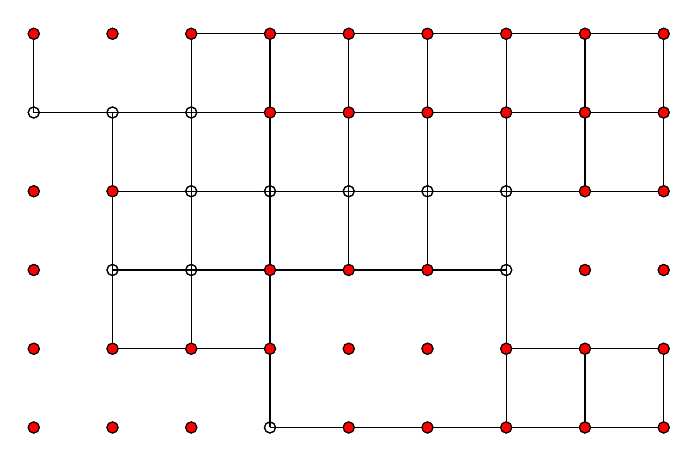
\begin{tikzpicture}[scale=1]%
\path[draw] (0.0,-8.0) -- (1.0,-8.0);%
\path[draw,radius=2pt] (0.0,-8.0) circle;%
\path[draw] (1.0,-8.0) -- (1.0,-9.0);%
\path[draw] (1.0,-8.0) -- (0.0,-8.0);%
\path[draw] (1.0,-8.0) -- (2.0,-8.0);%
\path[draw,radius=2pt] (1.0,-8.0) circle;%
\path[draw] (2.0,-8.0) -- (2.0,-9.0);%
\path[draw] (2.0,-8.0) -- (1.0,-8.0);%
\path[draw,radius=2pt] (2.0,-8.0) circle;%
\path[draw] (1.0,-9.0) -- (1.0,-8.0);%
\path[draw] (1.0,-9.0) -- (1.0,-10.0);%
\path[draw] (1.0,-9.0) -- (2.0,-9.0);%
\path[draw,radius=2pt] (1.0,-9.0) circle;%
\path[draw] (2.0,-9.0) -- (2.0,-8.0);%
\path[draw] (2.0,-9.0) -- (2.0,-10.0);%
\path[draw] (2.0,-9.0) -- (1.0,-9.0);%
\path[draw] (2.0,-9.0) -- (3.0,-9.0);%
\path[draw,radius=2pt] (2.0,-9.0) circle;%
\path[draw] (3.0,-9.0) -- (2.0,-9.0);%
\path[draw] (3.0,-9.0) -- (4.0,-9.0);%
\path[draw,radius=2pt] (3.0,-9.0) circle;%
\path[draw] (4.0,-9.0) -- (3.0,-9.0);%
\path[draw] (4.0,-9.0) -- (5.0,-9.0);%
\path[draw,radius=2pt] (4.0,-9.0) circle;%
\path[draw] (5.0,-9.0) -- (4.0,-9.0);%
\path[draw] (5.0,-9.0) -- (6.0,-9.0);%
\path[draw,radius=2pt] (5.0,-9.0) circle;%
\path[draw] (6.0,-9.0) -- (6.0,-10.0);%
\path[draw] (6.0,-9.0) -- (5.0,-9.0);%
\path[draw,radius=2pt] (6.0,-9.0) circle;%
\path[draw] (1.0,-10.0) -- (1.0,-9.0);%
\path[draw] (1.0,-10.0) -- (2.0,-10.0);%
\path[draw,radius=2pt] (1.0,-10.0) circle;%
\path[draw] (2.0,-10.0) -- (2.0,-9.0);%
\path[draw] (2.0,-10.0) -- (1.0,-10.0);%
\path[draw,radius=2pt] (2.0,-10.0) circle;%
\path[draw] (6.0,-10.0) -- (6.0,-9.0);%
\path[draw] (6.0,-10.0) -- (6.0,-11.0);%
\path[draw,radius=2pt] (6.0,-10.0) circle;%
\path[draw] (6.0,-11.0) -- (6.0,-10.0);%
\path[draw] (6.0,-11.0) -- (6.0,-12.0);%
\path[draw] (6.0,-11.0) -- (7.0,-11.0);%
\path[draw,radius=2pt] (6.0,-11.0) circle;%
\path[draw] (7.0,-11.0) -- (7.0,-12.0);%
\path[draw] (7.0,-11.0) -- (6.0,-11.0);%
\path[draw] (7.0,-11.0) -- (8.0,-11.0);%
\path[draw,radius=2pt] (7.0,-11.0) circle;%
\path[draw] (8.0,-11.0) -- (8.0,-12.0);%
\path[draw] (8.0,-11.0) -- (7.0,-11.0);%
\path[draw,radius=2pt] (8.0,-11.0) circle;%
\path[draw] (3.0,-12.0) -- (4.0,-12.0);%
\path[draw,radius=2pt] (3.0,-12.0) circle;%
\path[draw] (4.0,-12.0) -- (3.0,-12.0);%
\path[draw] (4.0,-12.0) -- (5.0,-12.0);%
\path[draw,radius=2pt] (4.0,-12.0) circle;%
\path[draw] (5.0,-12.0) -- (4.0,-12.0);%
\path[draw] (5.0,-12.0) -- (6.0,-12.0);%
\path[draw,radius=2pt] (5.0,-12.0) circle;%
\path[draw] (6.0,-12.0) -- (6.0,-11.0);%
\path[draw] (6.0,-12.0) -- (5.0,-12.0);%
\path[draw] (6.0,-12.0) -- (7.0,-12.0);%
\path[draw,radius=2pt] (6.0,-12.0) circle;%
\path[draw] (7.0,-12.0) -- (7.0,-11.0);%
\path[draw] (7.0,-12.0) -- (6.0,-12.0);%
\path[draw] (7.0,-12.0) -- (8.0,-12.0);%
\path[draw,radius=2pt] (7.0,-12.0) circle;%
\path[draw] (8.0,-12.0) -- (8.0,-11.0);%
\path[draw] (8.0,-12.0) -- (7.0,-12.0);%
\path[draw,radius=2pt] (8.0,-12.0) circle;%
\path[draw] (0.0,-7.0) -- (0.0,-8.0);%
\path[draw,radius=2pt] (0.0,-7.0) circle;%
\path[draw] (2.0,-7.0) -- (2.0,-8.0);%
\path[draw] (2.0,-7.0) -- (3.0,-7.0);%
\path[draw,radius=2pt] (2.0,-7.0) circle;%
\path[draw] (3.0,-7.0) -- (3.0,-8.0);%
\path[draw] (3.0,-7.0) -- (2.0,-7.0);%
\path[draw] (3.0,-7.0) -- (4.0,-7.0);%
\path[draw,radius=2pt] (3.0,-7.0) circle;%
\path[draw] (4.0,-7.0) -- (4.0,-8.0);%
\path[draw] (4.0,-7.0) -- (3.0,-7.0);%
\path[draw] (4.0,-7.0) -- (5.0,-7.0);%
\path[draw,radius=2pt] (4.0,-7.0) circle;%
\path[draw] (5.0,-7.0) -- (5.0,-8.0);%
\path[draw] (5.0,-7.0) -- (4.0,-7.0);%
\path[draw] (5.0,-7.0) -- (6.0,-7.0);%
\path[draw,radius=2pt] (5.0,-7.0) circle;%
\path[draw] (6.0,-7.0) -- (6.0,-8.0);%
\path[draw] (6.0,-7.0) -- (5.0,-7.0);%
\path[draw] (6.0,-7.0) -- (7.0,-7.0);%
\path[draw,radius=2pt] (6.0,-7.0) circle;%
\path[draw] (7.0,-7.0) -- (7.0,-8.0);%
\path[draw] (7.0,-7.0) -- (6.0,-7.0);%
\path[draw] (7.0,-7.0) -- (8.0,-7.0);%
\path[draw,radius=2pt] (7.0,-7.0) circle;%
\path[draw] (8.0,-7.0) -- (8.0,-8.0);%
\path[draw] (8.0,-7.0) -- (7.0,-7.0);%
\path[draw,radius=2pt] (8.0,-7.0) circle;%
\path[draw] (0.0,-8.0) -- (0.0,-7.0);%
\path[draw] (0.0,-8.0) -- (1.0,-8.0);%
\path[draw,radius=2pt] (0.0,-8.0) circle;%
\path[draw] (1.0,-8.0) -- (0.0,-8.0);%
\path[draw] (1.0,-8.0) -- (2.0,-8.0);%
\path[draw,radius=2pt] (1.0,-8.0) circle;%
\path[draw] (2.0,-8.0) -- (2.0,-7.0);%
\path[draw] (2.0,-8.0) -- (2.0,-9.0);%
\path[draw] (2.0,-8.0) -- (1.0,-8.0);%
\path[draw] (2.0,-8.0) -- (3.0,-8.0);%
\path[draw,radius=2pt] (2.0,-8.0) circle;%
\path[draw] (3.0,-8.0) -- (3.0,-7.0);%
\path[draw] (3.0,-8.0) -- (3.0,-9.0);%
\path[draw] (3.0,-8.0) -- (2.0,-8.0);%
\path[draw] (3.0,-8.0) -- (4.0,-8.0);%
\path[draw,radius=2pt] (3.0,-8.0) circle;%
\path[draw] (4.0,-8.0) -- (4.0,-7.0);%
\path[draw] (4.0,-8.0) -- (4.0,-9.0);%
\path[draw] (4.0,-8.0) -- (3.0,-8.0);%
\path[draw] (4.0,-8.0) -- (5.0,-8.0);%
\path[draw,radius=2pt] (4.0,-8.0) circle;%
\path[draw] (5.0,-8.0) -- (5.0,-7.0);%
\path[draw] (5.0,-8.0) -- (5.0,-9.0);%
\path[draw] (5.0,-8.0) -- (4.0,-8.0);%
\path[draw] (5.0,-8.0) -- (6.0,-8.0);%
\path[draw,radius=2pt] (5.0,-8.0) circle;%
\path[draw] (6.0,-8.0) -- (6.0,-7.0);%
\path[draw] (6.0,-8.0) -- (6.0,-9.0);%
\path[draw] (6.0,-8.0) -- (5.0,-8.0);%
\path[draw] (6.0,-8.0) -- (7.0,-8.0);%
\path[draw,radius=2pt] (6.0,-8.0) circle;%
\path[draw] (7.0,-8.0) -- (7.0,-7.0);%
\path[draw] (7.0,-8.0) -- (7.0,-9.0);%
\path[draw] (7.0,-8.0) -- (6.0,-8.0);%
\path[draw] (7.0,-8.0) -- (8.0,-8.0);%
\path[draw,radius=2pt] (7.0,-8.0) circle;%
\path[draw] (8.0,-8.0) -- (8.0,-7.0);%
\path[draw] (8.0,-8.0) -- (8.0,-9.0);%
\path[draw] (8.0,-8.0) -- (7.0,-8.0);%
\path[draw,radius=2pt] (8.0,-8.0) circle;%
\path[draw] (2.0,-9.0) -- (2.0,-8.0);%
\path[draw] (2.0,-9.0) -- (2.0,-10.0);%
\path[draw] (2.0,-9.0) -- (3.0,-9.0);%
\path[draw,radius=2pt] (2.0,-9.0) circle;%
\path[draw] (3.0,-9.0) -- (3.0,-8.0);%
\path[draw] (3.0,-9.0) -- (3.0,-10.0);%
\path[draw] (3.0,-9.0) -- (2.0,-9.0);%
\path[draw] (3.0,-9.0) -- (4.0,-9.0);%
\path[draw,radius=2pt] (3.0,-9.0) circle;%
\path[draw] (4.0,-9.0) -- (4.0,-8.0);%
\path[draw] (4.0,-9.0) -- (4.0,-10.0);%
\path[draw] (4.0,-9.0) -- (3.0,-9.0);%
\path[draw] (4.0,-9.0) -- (5.0,-9.0);%
\path[draw,radius=2pt] (4.0,-9.0) circle;%
\path[draw] (5.0,-9.0) -- (5.0,-8.0);%
\path[draw] (5.0,-9.0) -- (5.0,-10.0);%
\path[draw] (5.0,-9.0) -- (4.0,-9.0);%
\path[draw] (5.0,-9.0) -- (6.0,-9.0);%
\path[draw,radius=2pt] (5.0,-9.0) circle;%
\path[draw] (6.0,-9.0) -- (6.0,-8.0);%
\path[draw] (6.0,-9.0) -- (6.0,-10.0);%
\path[draw] (6.0,-9.0) -- (5.0,-9.0);%
\path[draw] (6.0,-9.0) -- (7.0,-9.0);%
\path[draw,radius=2pt] (6.0,-9.0) circle;%
\path[draw] (7.0,-9.0) -- (7.0,-8.0);%
\path[draw] (7.0,-9.0) -- (6.0,-9.0);%
\path[draw] (7.0,-9.0) -- (8.0,-9.0);%
\path[draw,radius=2pt] (7.0,-9.0) circle;%
\path[draw] (8.0,-9.0) -- (8.0,-8.0);%
\path[draw] (8.0,-9.0) -- (7.0,-9.0);%
\path[draw,radius=2pt] (8.0,-9.0) circle;%
\path[draw] (1.0,-10.0) -- (1.0,-11.0);%
\path[draw] (1.0,-10.0) -- (2.0,-10.0);%
\path[draw,radius=2pt] (1.0,-10.0) circle;%
\path[draw] (2.0,-10.0) -- (2.0,-9.0);%
\path[draw] (2.0,-10.0) -- (2.0,-11.0);%
\path[draw] (2.0,-10.0) -- (1.0,-10.0);%
\path[draw] (2.0,-10.0) -- (3.0,-10.0);%
\path[draw,radius=2pt] (2.0,-10.0) circle;%
\path[draw] (3.0,-10.0) -- (3.0,-9.0);%
\path[draw] (3.0,-10.0) -- (3.0,-11.0);%
\path[draw] (3.0,-10.0) -- (2.0,-10.0);%
\path[draw] (3.0,-10.0) -- (4.0,-10.0);%
\path[draw,radius=2pt] (3.0,-10.0) circle;%
\path[draw] (4.0,-10.0) -- (4.0,-9.0);%
\path[draw] (4.0,-10.0) -- (3.0,-10.0);%
\path[draw] (4.0,-10.0) -- (5.0,-10.0);%
\path[draw,radius=2pt] (4.0,-10.0) circle;%
\path[draw] (5.0,-10.0) -- (5.0,-9.0);%
\path[draw] (5.0,-10.0) -- (4.0,-10.0);%
\path[draw] (5.0,-10.0) -- (6.0,-10.0);%
\path[draw,radius=2pt] (5.0,-10.0) circle;%
\path[draw] (6.0,-10.0) -- (6.0,-9.0);%
\path[draw] (6.0,-10.0) -- (5.0,-10.0);%
\path[draw,radius=2pt] (6.0,-10.0) circle;%
\path[draw] (1.0,-11.0) -- (1.0,-10.0);%
\path[draw] (1.0,-11.0) -- (2.0,-11.0);%
\path[draw,radius=2pt] (1.0,-11.0) circle;%
\path[draw] (2.0,-11.0) -- (2.0,-10.0);%
\path[draw] (2.0,-11.0) -- (1.0,-11.0);%
\path[draw] (2.0,-11.0) -- (3.0,-11.0);%
\path[draw,radius=2pt] (2.0,-11.0) circle;%
\path[draw] (3.0,-11.0) -- (3.0,-10.0);%
\path[draw] (3.0,-11.0) -- (3.0,-12.0);%
\path[draw] (3.0,-11.0) -- (2.0,-11.0);%
\path[draw,radius=2pt] (3.0,-11.0) circle;%
\path[draw] (3.0,-12.0) -- (3.0,-11.0);%
\path[draw,radius=2pt] (3.0,-12.0) circle;%
\path[draw,radius=2pt,fill=red] (0.0,-7.0) circle;%
\path[draw,radius=2pt,fill=red] (1.0,-7.0) circle;%
\path[draw,radius=2pt,fill=red] (2.0,-7.0) circle;%
\path[draw,radius=2pt,fill=red] (3.0,-7.0) circle;%
\path[draw,radius=2pt,fill=red] (4.0,-7.0) circle;%
\path[draw,radius=2pt,fill=red] (5.0,-7.0) circle;%
\path[draw,radius=2pt,fill=red] (6.0,-7.0) circle;%
\path[draw,radius=2pt,fill=red] (7.0,-7.0) circle;%
\path[draw,radius=2pt,fill=red] (8.0,-7.0) circle;%
\path[draw,radius=2pt,fill=red] (3.0,-8.0) circle;%
\path[draw,radius=2pt,fill=red] (4.0,-8.0) circle;%
\path[draw,radius=2pt,fill=red] (5.0,-8.0) circle;%
\path[draw,radius=2pt,fill=red] (6.0,-8.0) circle;%
\path[draw,radius=2pt,fill=red] (7.0,-8.0) circle;%
\path[draw,radius=2pt,fill=red] (8.0,-8.0) circle;%
\path[draw,radius=2pt,fill=red] (0.0,-9.0) circle;%
\path[draw,radius=2pt,fill=red] (7.0,-9.0) circle;%
\path[draw,radius=2pt,fill=red] (8.0,-9.0) circle;%
\path[draw,radius=2pt,fill=red] (0.0,-10.0) circle;%
\path[draw,radius=2pt,fill=red] (3.0,-10.0) circle;%
\path[draw,radius=2pt,fill=red] (4.0,-10.0) circle;%
\path[draw,radius=2pt,fill=red] (5.0,-10.0) circle;%
\path[draw,radius=2pt,fill=red] (7.0,-10.0) circle;%
\path[draw,radius=2pt,fill=red] (8.0,-10.0) circle;%
\path[draw,radius=2pt,fill=red] (0.0,-11.0) circle;%
\path[draw,radius=2pt,fill=red] (1.0,-11.0) circle;%
\path[draw,radius=2pt,fill=red] (2.0,-11.0) circle;%
\path[draw,radius=2pt,fill=red] (3.0,-11.0) circle;%
\path[draw,radius=2pt,fill=red] (4.0,-11.0) circle;%
\path[draw,radius=2pt,fill=red] (5.0,-11.0) circle;%
\path[draw,radius=2pt,fill=red] (0.0,-12.0) circle;%
\path[draw,radius=2pt,fill=red] (1.0,-12.0) circle;%
\path[draw,radius=2pt,fill=red] (2.0,-12.0) circle;%
\path[draw,radius=2pt,fill=red] (1.0,-7.0) circle;%
\path[draw,radius=2pt,fill=red] (0.0,-9.0) circle;%
\path[draw,radius=2pt,fill=red] (1.0,-9.0) circle;%
\path[draw,radius=2pt,fill=red] (0.0,-10.0) circle;%
\path[draw,radius=2pt,fill=red] (7.0,-10.0) circle;%
\path[draw,radius=2pt,fill=red] (8.0,-10.0) circle;%
\path[draw,radius=2pt,fill=red] (0.0,-11.0) circle;%
\path[draw,radius=2pt,fill=red] (4.0,-11.0) circle;%
\path[draw,radius=2pt,fill=red] (5.0,-11.0) circle;%
\path[draw,radius=2pt,fill=red] (6.0,-11.0) circle;%
\path[draw,radius=2pt,fill=red] (7.0,-11.0) circle;%
\path[draw,radius=2pt,fill=red] (8.0,-11.0) circle;%
\path[draw,radius=2pt,fill=red] (0.0,-12.0) circle;%
\path[draw,radius=2pt,fill=red] (1.0,-12.0) circle;%
\path[draw,radius=2pt,fill=red] (2.0,-12.0) circle;%
\path[draw,radius=2pt,fill=red] (4.0,-12.0) circle;%
\path[draw,radius=2pt,fill=red] (5.0,-12.0) circle;%
\path[draw,radius=2pt,fill=red] (6.0,-12.0) circle;%
\path[draw,radius=2pt,fill=red] (7.0,-12.0) circle;%
\path[draw,radius=2pt,fill=red] (8.0,-12.0) circle;%
\end{tikzpicture}%
\newline%
\hspace*{1in}%
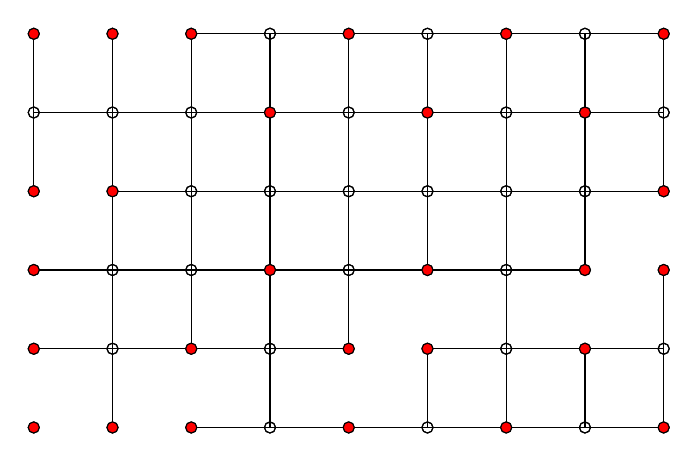
\begin{tikzpicture}[scale=1]%
\path[draw] (1.0,-7.0) -- (1.0,-8.0);%
\path[draw,radius=2pt] (1.0,-7.0) circle;%
\path[draw,radius=2pt] (3.0,-7.0) circle;%
\path[draw,radius=2pt] (5.0,-7.0) circle;%
\path[draw,radius=2pt] (7.0,-7.0) circle;%
\path[draw] (0.0,-8.0) -- (1.0,-8.0);%
\path[draw,radius=2pt] (0.0,-8.0) circle;%
\path[draw] (1.0,-8.0) -- (1.0,-7.0);%
\path[draw] (1.0,-8.0) -- (1.0,-9.0);%
\path[draw] (1.0,-8.0) -- (0.0,-8.0);%
\path[draw] (1.0,-8.0) -- (2.0,-8.0);%
\path[draw,radius=2pt] (1.0,-8.0) circle;%
\path[draw] (2.0,-8.0) -- (2.0,-9.0);%
\path[draw] (2.0,-8.0) -- (1.0,-8.0);%
\path[draw,radius=2pt] (2.0,-8.0) circle;%
\path[draw] (4.0,-8.0) -- (4.0,-9.0);%
\path[draw,radius=2pt] (4.0,-8.0) circle;%
\path[draw] (6.0,-8.0) -- (6.0,-9.0);%
\path[draw,radius=2pt] (6.0,-8.0) circle;%
\path[draw,radius=2pt] (8.0,-8.0) circle;%
\path[draw] (1.0,-9.0) -- (1.0,-8.0);%
\path[draw] (1.0,-9.0) -- (1.0,-10.0);%
\path[draw] (1.0,-9.0) -- (2.0,-9.0);%
\path[draw,radius=2pt] (1.0,-9.0) circle;%
\path[draw] (2.0,-9.0) -- (2.0,-8.0);%
\path[draw] (2.0,-9.0) -- (2.0,-10.0);%
\path[draw] (2.0,-9.0) -- (1.0,-9.0);%
\path[draw] (2.0,-9.0) -- (3.0,-9.0);%
\path[draw,radius=2pt] (2.0,-9.0) circle;%
\path[draw] (3.0,-9.0) -- (2.0,-9.0);%
\path[draw] (3.0,-9.0) -- (4.0,-9.0);%
\path[draw,radius=2pt] (3.0,-9.0) circle;%
\path[draw] (4.0,-9.0) -- (4.0,-8.0);%
\path[draw] (4.0,-9.0) -- (4.0,-10.0);%
\path[draw] (4.0,-9.0) -- (3.0,-9.0);%
\path[draw] (4.0,-9.0) -- (5.0,-9.0);%
\path[draw,radius=2pt] (4.0,-9.0) circle;%
\path[draw] (5.0,-9.0) -- (4.0,-9.0);%
\path[draw] (5.0,-9.0) -- (6.0,-9.0);%
\path[draw,radius=2pt] (5.0,-9.0) circle;%
\path[draw] (6.0,-9.0) -- (6.0,-8.0);%
\path[draw] (6.0,-9.0) -- (6.0,-10.0);%
\path[draw] (6.0,-9.0) -- (5.0,-9.0);%
\path[draw] (6.0,-9.0) -- (7.0,-9.0);%
\path[draw,radius=2pt] (6.0,-9.0) circle;%
\path[draw] (7.0,-9.0) -- (6.0,-9.0);%
\path[draw,radius=2pt] (7.0,-9.0) circle;%
\path[draw] (0.0,-10.0) -- (1.0,-10.0);%
\path[draw,radius=2pt] (0.0,-10.0) circle;%
\path[draw] (1.0,-10.0) -- (1.0,-9.0);%
\path[draw] (1.0,-10.0) -- (1.0,-11.0);%
\path[draw] (1.0,-10.0) -- (0.0,-10.0);%
\path[draw] (1.0,-10.0) -- (2.0,-10.0);%
\path[draw,radius=2pt] (1.0,-10.0) circle;%
\path[draw] (2.0,-10.0) -- (2.0,-9.0);%
\path[draw] (2.0,-10.0) -- (1.0,-10.0);%
\path[draw,radius=2pt] (2.0,-10.0) circle;%
\path[draw] (4.0,-10.0) -- (4.0,-9.0);%
\path[draw,radius=2pt] (4.0,-10.0) circle;%
\path[draw] (6.0,-10.0) -- (6.0,-9.0);%
\path[draw] (6.0,-10.0) -- (6.0,-11.0);%
\path[draw,radius=2pt] (6.0,-10.0) circle;%
\path[draw] (8.0,-10.0) -- (8.0,-11.0);%
\path[draw,radius=2pt] (8.0,-10.0) circle;%
\path[draw] (1.0,-11.0) -- (1.0,-10.0);%
\path[draw,radius=2pt] (1.0,-11.0) circle;%
\path[draw] (3.0,-11.0) -- (3.0,-12.0);%
\path[draw,radius=2pt] (3.0,-11.0) circle;%
\path[draw] (5.0,-11.0) -- (5.0,-12.0);%
\path[draw] (5.0,-11.0) -- (6.0,-11.0);%
\path[draw,radius=2pt] (5.0,-11.0) circle;%
\path[draw] (6.0,-11.0) -- (6.0,-10.0);%
\path[draw] (6.0,-11.0) -- (6.0,-12.0);%
\path[draw] (6.0,-11.0) -- (5.0,-11.0);%
\path[draw] (6.0,-11.0) -- (7.0,-11.0);%
\path[draw,radius=2pt] (6.0,-11.0) circle;%
\path[draw] (7.0,-11.0) -- (7.0,-12.0);%
\path[draw] (7.0,-11.0) -- (6.0,-11.0);%
\path[draw] (7.0,-11.0) -- (8.0,-11.0);%
\path[draw,radius=2pt] (7.0,-11.0) circle;%
\path[draw] (8.0,-11.0) -- (8.0,-10.0);%
\path[draw] (8.0,-11.0) -- (8.0,-12.0);%
\path[draw] (8.0,-11.0) -- (7.0,-11.0);%
\path[draw,radius=2pt] (8.0,-11.0) circle;%
\path[draw,radius=2pt] (0.0,-12.0) circle;%
\path[draw] (2.0,-12.0) -- (3.0,-12.0);%
\path[draw,radius=2pt] (2.0,-12.0) circle;%
\path[draw] (3.0,-12.0) -- (3.0,-11.0);%
\path[draw] (3.0,-12.0) -- (2.0,-12.0);%
\path[draw] (3.0,-12.0) -- (4.0,-12.0);%
\path[draw,radius=2pt] (3.0,-12.0) circle;%
\path[draw] (4.0,-12.0) -- (3.0,-12.0);%
\path[draw] (4.0,-12.0) -- (5.0,-12.0);%
\path[draw,radius=2pt] (4.0,-12.0) circle;%
\path[draw] (5.0,-12.0) -- (5.0,-11.0);%
\path[draw] (5.0,-12.0) -- (4.0,-12.0);%
\path[draw] (5.0,-12.0) -- (6.0,-12.0);%
\path[draw,radius=2pt] (5.0,-12.0) circle;%
\path[draw] (6.0,-12.0) -- (6.0,-11.0);%
\path[draw] (6.0,-12.0) -- (5.0,-12.0);%
\path[draw] (6.0,-12.0) -- (7.0,-12.0);%
\path[draw,radius=2pt] (6.0,-12.0) circle;%
\path[draw] (7.0,-12.0) -- (7.0,-11.0);%
\path[draw] (7.0,-12.0) -- (6.0,-12.0);%
\path[draw] (7.0,-12.0) -- (8.0,-12.0);%
\path[draw,radius=2pt] (7.0,-12.0) circle;%
\path[draw] (8.0,-12.0) -- (8.0,-11.0);%
\path[draw] (8.0,-12.0) -- (7.0,-12.0);%
\path[draw,radius=2pt] (8.0,-12.0) circle;%
\path[draw] (0.0,-7.0) -- (0.0,-8.0);%
\path[draw,radius=2pt] (0.0,-7.0) circle;%
\path[draw] (2.0,-7.0) -- (2.0,-8.0);%
\path[draw] (2.0,-7.0) -- (3.0,-7.0);%
\path[draw,radius=2pt] (2.0,-7.0) circle;%
\path[draw] (3.0,-7.0) -- (3.0,-8.0);%
\path[draw] (3.0,-7.0) -- (2.0,-7.0);%
\path[draw] (3.0,-7.0) -- (4.0,-7.0);%
\path[draw,radius=2pt] (3.0,-7.0) circle;%
\path[draw] (4.0,-7.0) -- (4.0,-8.0);%
\path[draw] (4.0,-7.0) -- (3.0,-7.0);%
\path[draw] (4.0,-7.0) -- (5.0,-7.0);%
\path[draw,radius=2pt] (4.0,-7.0) circle;%
\path[draw] (5.0,-7.0) -- (5.0,-8.0);%
\path[draw] (5.0,-7.0) -- (4.0,-7.0);%
\path[draw] (5.0,-7.0) -- (6.0,-7.0);%
\path[draw,radius=2pt] (5.0,-7.0) circle;%
\path[draw] (6.0,-7.0) -- (6.0,-8.0);%
\path[draw] (6.0,-7.0) -- (5.0,-7.0);%
\path[draw] (6.0,-7.0) -- (7.0,-7.0);%
\path[draw,radius=2pt] (6.0,-7.0) circle;%
\path[draw] (7.0,-7.0) -- (7.0,-8.0);%
\path[draw] (7.0,-7.0) -- (6.0,-7.0);%
\path[draw] (7.0,-7.0) -- (8.0,-7.0);%
\path[draw,radius=2pt] (7.0,-7.0) circle;%
\path[draw] (8.0,-7.0) -- (8.0,-8.0);%
\path[draw] (8.0,-7.0) -- (7.0,-7.0);%
\path[draw,radius=2pt] (8.0,-7.0) circle;%
\path[draw] (0.0,-8.0) -- (0.0,-7.0);%
\path[draw] (0.0,-8.0) -- (0.0,-9.0);%
\path[draw] (0.0,-8.0) -- (1.0,-8.0);%
\path[draw,radius=2pt] (0.0,-8.0) circle;%
\path[draw] (1.0,-8.0) -- (0.0,-8.0);%
\path[draw] (1.0,-8.0) -- (2.0,-8.0);%
\path[draw,radius=2pt] (1.0,-8.0) circle;%
\path[draw] (2.0,-8.0) -- (2.0,-7.0);%
\path[draw] (2.0,-8.0) -- (2.0,-9.0);%
\path[draw] (2.0,-8.0) -- (1.0,-8.0);%
\path[draw] (2.0,-8.0) -- (3.0,-8.0);%
\path[draw,radius=2pt] (2.0,-8.0) circle;%
\path[draw] (3.0,-8.0) -- (3.0,-7.0);%
\path[draw] (3.0,-8.0) -- (3.0,-9.0);%
\path[draw] (3.0,-8.0) -- (2.0,-8.0);%
\path[draw] (3.0,-8.0) -- (4.0,-8.0);%
\path[draw,radius=2pt] (3.0,-8.0) circle;%
\path[draw] (4.0,-8.0) -- (4.0,-7.0);%
\path[draw] (4.0,-8.0) -- (4.0,-9.0);%
\path[draw] (4.0,-8.0) -- (3.0,-8.0);%
\path[draw] (4.0,-8.0) -- (5.0,-8.0);%
\path[draw,radius=2pt] (4.0,-8.0) circle;%
\path[draw] (5.0,-8.0) -- (5.0,-7.0);%
\path[draw] (5.0,-8.0) -- (5.0,-9.0);%
\path[draw] (5.0,-8.0) -- (4.0,-8.0);%
\path[draw] (5.0,-8.0) -- (6.0,-8.0);%
\path[draw,radius=2pt] (5.0,-8.0) circle;%
\path[draw] (6.0,-8.0) -- (6.0,-7.0);%
\path[draw] (6.0,-8.0) -- (6.0,-9.0);%
\path[draw] (6.0,-8.0) -- (5.0,-8.0);%
\path[draw] (6.0,-8.0) -- (7.0,-8.0);%
\path[draw,radius=2pt] (6.0,-8.0) circle;%
\path[draw] (7.0,-8.0) -- (7.0,-7.0);%
\path[draw] (7.0,-8.0) -- (7.0,-9.0);%
\path[draw] (7.0,-8.0) -- (6.0,-8.0);%
\path[draw] (7.0,-8.0) -- (8.0,-8.0);%
\path[draw,radius=2pt] (7.0,-8.0) circle;%
\path[draw] (8.0,-8.0) -- (8.0,-7.0);%
\path[draw] (8.0,-8.0) -- (8.0,-9.0);%
\path[draw] (8.0,-8.0) -- (7.0,-8.0);%
\path[draw,radius=2pt] (8.0,-8.0) circle;%
\path[draw] (0.0,-9.0) -- (0.0,-8.0);%
\path[draw,radius=2pt] (0.0,-9.0) circle;%
\path[draw] (2.0,-9.0) -- (2.0,-8.0);%
\path[draw] (2.0,-9.0) -- (2.0,-10.0);%
\path[draw] (2.0,-9.0) -- (3.0,-9.0);%
\path[draw,radius=2pt] (2.0,-9.0) circle;%
\path[draw] (3.0,-9.0) -- (3.0,-8.0);%
\path[draw] (3.0,-9.0) -- (3.0,-10.0);%
\path[draw] (3.0,-9.0) -- (2.0,-9.0);%
\path[draw] (3.0,-9.0) -- (4.0,-9.0);%
\path[draw,radius=2pt] (3.0,-9.0) circle;%
\path[draw] (4.0,-9.0) -- (4.0,-8.0);%
\path[draw] (4.0,-9.0) -- (4.0,-10.0);%
\path[draw] (4.0,-9.0) -- (3.0,-9.0);%
\path[draw] (4.0,-9.0) -- (5.0,-9.0);%
\path[draw,radius=2pt] (4.0,-9.0) circle;%
\path[draw] (5.0,-9.0) -- (5.0,-8.0);%
\path[draw] (5.0,-9.0) -- (5.0,-10.0);%
\path[draw] (5.0,-9.0) -- (4.0,-9.0);%
\path[draw] (5.0,-9.0) -- (6.0,-9.0);%
\path[draw,radius=2pt] (5.0,-9.0) circle;%
\path[draw] (6.0,-9.0) -- (6.0,-8.0);%
\path[draw] (6.0,-9.0) -- (6.0,-10.0);%
\path[draw] (6.0,-9.0) -- (5.0,-9.0);%
\path[draw] (6.0,-9.0) -- (7.0,-9.0);%
\path[draw,radius=2pt] (6.0,-9.0) circle;%
\path[draw] (7.0,-9.0) -- (7.0,-8.0);%
\path[draw] (7.0,-9.0) -- (7.0,-10.0);%
\path[draw] (7.0,-9.0) -- (6.0,-9.0);%
\path[draw] (7.0,-9.0) -- (8.0,-9.0);%
\path[draw,radius=2pt] (7.0,-9.0) circle;%
\path[draw] (8.0,-9.0) -- (8.0,-8.0);%
\path[draw] (8.0,-9.0) -- (7.0,-9.0);%
\path[draw,radius=2pt] (8.0,-9.0) circle;%
\path[draw] (1.0,-10.0) -- (1.0,-11.0);%
\path[draw] (1.0,-10.0) -- (2.0,-10.0);%
\path[draw,radius=2pt] (1.0,-10.0) circle;%
\path[draw] (2.0,-10.0) -- (2.0,-9.0);%
\path[draw] (2.0,-10.0) -- (2.0,-11.0);%
\path[draw] (2.0,-10.0) -- (1.0,-10.0);%
\path[draw] (2.0,-10.0) -- (3.0,-10.0);%
\path[draw,radius=2pt] (2.0,-10.0) circle;%
\path[draw] (3.0,-10.0) -- (3.0,-9.0);%
\path[draw] (3.0,-10.0) -- (3.0,-11.0);%
\path[draw] (3.0,-10.0) -- (2.0,-10.0);%
\path[draw] (3.0,-10.0) -- (4.0,-10.0);%
\path[draw,radius=2pt] (3.0,-10.0) circle;%
\path[draw] (4.0,-10.0) -- (4.0,-9.0);%
\path[draw] (4.0,-10.0) -- (4.0,-11.0);%
\path[draw] (4.0,-10.0) -- (3.0,-10.0);%
\path[draw] (4.0,-10.0) -- (5.0,-10.0);%
\path[draw,radius=2pt] (4.0,-10.0) circle;%
\path[draw] (5.0,-10.0) -- (5.0,-9.0);%
\path[draw] (5.0,-10.0) -- (4.0,-10.0);%
\path[draw] (5.0,-10.0) -- (6.0,-10.0);%
\path[draw,radius=2pt] (5.0,-10.0) circle;%
\path[draw] (6.0,-10.0) -- (6.0,-9.0);%
\path[draw] (6.0,-10.0) -- (6.0,-11.0);%
\path[draw] (6.0,-10.0) -- (5.0,-10.0);%
\path[draw] (6.0,-10.0) -- (7.0,-10.0);%
\path[draw,radius=2pt] (6.0,-10.0) circle;%
\path[draw] (7.0,-10.0) -- (7.0,-9.0);%
\path[draw] (7.0,-10.0) -- (6.0,-10.0);%
\path[draw,radius=2pt] (7.0,-10.0) circle;%
\path[draw] (0.0,-11.0) -- (1.0,-11.0);%
\path[draw,radius=2pt] (0.0,-11.0) circle;%
\path[draw] (1.0,-11.0) -- (1.0,-10.0);%
\path[draw] (1.0,-11.0) -- (1.0,-12.0);%
\path[draw] (1.0,-11.0) -- (0.0,-11.0);%
\path[draw] (1.0,-11.0) -- (2.0,-11.0);%
\path[draw,radius=2pt] (1.0,-11.0) circle;%
\path[draw] (2.0,-11.0) -- (2.0,-10.0);%
\path[draw] (2.0,-11.0) -- (1.0,-11.0);%
\path[draw] (2.0,-11.0) -- (3.0,-11.0);%
\path[draw,radius=2pt] (2.0,-11.0) circle;%
\path[draw] (3.0,-11.0) -- (3.0,-10.0);%
\path[draw] (3.0,-11.0) -- (3.0,-12.0);%
\path[draw] (3.0,-11.0) -- (2.0,-11.0);%
\path[draw] (3.0,-11.0) -- (4.0,-11.0);%
\path[draw,radius=2pt] (3.0,-11.0) circle;%
\path[draw] (4.0,-11.0) -- (4.0,-10.0);%
\path[draw] (4.0,-11.0) -- (3.0,-11.0);%
\path[draw,radius=2pt] (4.0,-11.0) circle;%
\path[draw] (6.0,-11.0) -- (6.0,-10.0);%
\path[draw,radius=2pt] (6.0,-11.0) circle;%
\path[draw,radius=2pt] (8.0,-11.0) circle;%
\path[draw] (1.0,-12.0) -- (1.0,-11.0);%
\path[draw,radius=2pt] (1.0,-12.0) circle;%
\path[draw] (3.0,-12.0) -- (3.0,-11.0);%
\path[draw,radius=2pt] (3.0,-12.0) circle;%
\path[draw,radius=2pt] (5.0,-12.0) circle;%
\path[draw,radius=2pt] (7.0,-12.0) circle;%
\path[draw,radius=2pt,fill=red] (0.0,-7.0) circle;%
\path[draw,radius=2pt,fill=red] (2.0,-7.0) circle;%
\path[draw,radius=2pt,fill=red] (4.0,-7.0) circle;%
\path[draw,radius=2pt,fill=red] (6.0,-7.0) circle;%
\path[draw,radius=2pt,fill=red] (8.0,-7.0) circle;%
\path[draw,radius=2pt,fill=red] (3.0,-8.0) circle;%
\path[draw,radius=2pt,fill=red] (5.0,-8.0) circle;%
\path[draw,radius=2pt,fill=red] (7.0,-8.0) circle;%
\path[draw,radius=2pt,fill=red] (0.0,-9.0) circle;%
\path[draw,radius=2pt,fill=red] (8.0,-9.0) circle;%
\path[draw,radius=2pt,fill=red] (3.0,-10.0) circle;%
\path[draw,radius=2pt,fill=red] (5.0,-10.0) circle;%
\path[draw,radius=2pt,fill=red] (7.0,-10.0) circle;%
\path[draw,radius=2pt,fill=red] (0.0,-11.0) circle;%
\path[draw,radius=2pt,fill=red] (2.0,-11.0) circle;%
\path[draw,radius=2pt,fill=red] (4.0,-11.0) circle;%
\path[draw,radius=2pt,fill=red] (1.0,-12.0) circle;%
\path[draw,radius=2pt,fill=red] (1.0,-7.0) circle;%
\path[draw,radius=2pt,fill=red] (1.0,-9.0) circle;%
\path[draw,radius=2pt,fill=red] (0.0,-10.0) circle;%
\path[draw,radius=2pt,fill=red] (8.0,-10.0) circle;%
\path[draw,radius=2pt,fill=red] (5.0,-11.0) circle;%
\path[draw,radius=2pt,fill=red] (7.0,-11.0) circle;%
\path[draw,radius=2pt,fill=red] (0.0,-12.0) circle;%
\path[draw,radius=2pt,fill=red] (2.0,-12.0) circle;%
\path[draw,radius=2pt,fill=red] (4.0,-12.0) circle;%
\path[draw,radius=2pt,fill=red] (6.0,-12.0) circle;%
\path[draw,radius=2pt,fill=red] (8.0,-12.0) circle;%
\end{tikzpicture}%
\end{document}